\documentclass[12pt,twoside=false,openright,numbers=noenddot]{scrbook}
\usepackage{evan}
\usepackage{addons}
\usepackage{amsmath,amsthm,xfrac,amssymb}


\newcommand{\Z}{\mathbb{Z}}
\newcommand{\U}{\mathbb{U}}
\newcommand{\Q}{\mathbb{Q}}
\newcommand{\N}{\mathbb{N}}
\newcommand{\la}{\langle}
\newcommand{\ra}{\rangle}


\newcommand{\pp}{^{-1}}
\newcommand{\ee}{\epsilon}
\newcommand{\pd}[2]{\frac{\partial #1}{\partial #2}}
\newcommand{\La}{\mathcal{L}}
\newcommand{\gaa}{\gamma}

\newcommand{\bias}{\textnormal{bias}}
\newcommand{\mse}{\textnormal{mse}}
\newcommand{\ttt}{\theta}
\newcommand{\vvv}{\mathcal{v}}
\newcommand{\cond}{\xrightarrow{d}}
\newcommand{\conp}{\xrightarrow{p}}
\newcommand{\Ex}{\mathrm{E}}
\newcommand{\htt}{\hat{\theta}}
\newcommand{\tth}{\tilde{\theta}}
\usepackage{setspace}
\usepackage{xcolor}
\definecolor{timGreen}{RGB}{0,79,12}
\definecolor{Cites}{RGB}{62,62,199}
%\usepackage[numbers]{natbib}888
\usepackage{natbib}
\bibliographystyle{chicago}
\usepackage[english]{babel}
\usepackage{hyperref}
\hypersetup{
    colorlinks=true,
    linkcolor=blue,
    filecolor=blue,
    urlcolor=blue,
    citecolor = Cites
}
\onehalfspacing
\title{Economics 1011A Textbook}
\subtitle{Based on class by Prof. Edward L. Glaeser\footnote{Most recent version \href{https://github.com/tim-hua-01/ECON-1011A-Textbook/blob/master/textbook.pdf}{here}. \newline Reach out to Tim.Hua@Walmart.com for textbook-related questions.} }
\author{Kevin Bi, Jimmy Lin, and Tim Hua}


\begin{document}

% \frontmatter
% \renewcommand{\thepage}{\arabic{page}}
\maketitle
\tableofcontents

\part{Introduction}
% Fyi, I've read online that include is better than input
\chapter{Economic Modeling Overview}

\section{What is Economic Modeling?}
The goal of an economic model is to take some real world phenomena and represent it in a way that we can analyze it rigorously and tractably. At the most fundamental level, a \vocab{model} is just a set of assumptions that we make. Models can take many forms, and you are likely already familiar with some models of real world phenomena. For example, you might construct a model of dining preferences by assuming that the number of people who eat in the dining halls is greater on days where the food is good. Or you might have seen toy models of molecules where the atoms are represented by marshmallows and the bonds between them as toothpicks. With the COVID-19 pandemic, models of infectious disease were used to predict the future number of infectious by assuming how often people interacted with each other,  

Economic models try to answer economic questions. Some of these questions might include:
\begin{itemize}
    \item How does the minimum wage affect the amount of labor hired?
    \item What is the tax rate that maximizes revenue for the government?
    \item How does the interest rate affect savings and investment?
\end{itemize}
Importantly, economic models usually focus on \vocab{positive} economic questions, that is questions about how things in the world work. This is contrast to \vocab{normative} economics, which answers how things should be. However, that does not mean that economic models cannot tell us the optimal policy. While an economic model cannot answer what the `best' policy is in a vaccum, it can tell us what the best policy is once we have defined what `best' means. Normative economics examines what it means for a policy to be the `best,' while positive economics tells us how we get there.

A model can take many forms, but in this class, we focus on mathematical models of economic behavior. That is, we try to represent the behavior of people, firms, and governments via mathematical functions and see what insights can be gained from such representation. The use of mathematics allows us to formalize our economic reasoning and make precise what conclusions must follow from certain assumptions. 

\subsection*{What makes a good economic model?}
As you will learn throughout this course, economic models can take many forms and there is almost no limit to the models that you can create. However, just because you can write down a certain model, does not mean that model is a good one. Most good economic models share a few key characteristics:
\begin{itemize}
    \item A model should make clear what assumptions are being included, how these assumptions affect the model's conclusions, and the potential limitations of these assumptions.
    \item A model should be general enough to be a realistic representation of the real world but also simple enough to be easy to manipulate and interpret mathematically. Striking this balance will be a key theme of this course and will be important for doing well in each of the modeling projects.
    \item The conclusions of a model should tie back to the problem being asked. Deriving a mathematical expression that quantifies a particular behavior or result is often the majority of the battle, but it is important to understand how these results answer our initial question and whether our interpretation makes sense intuitively.
\end{itemize}

\subsection*{The role of assumptions}
You may have heard that economists make unrealistic assumptions in their models, and to a certain degree this is true. Most economists do not think that individuals or even firms are actually able to perfectly optimize their decisions. However, since the real world is too complex to model perfectly, assumptions play a few crucial roles: 
\begin{description}
    \item[Tractability] Perhaps the main role of assumptions is to make models tractable to solve analytically. It would be almost impossible to make concise models that generate useful predictions if we had to figure out how every person in the world makes decisions. Assumptions allow us to simplify the model so that they can actually be solved with current mathematical techniques.
    \item[Illustrate possibility] Related to the tractability rationale for models, we may make assumptions to show that certain mechanics are at least possible under assumptions that are not too unreasonable. The assumptions allow us to simplify the problem so that the mechanisms are more clear, and helps us obtain a better understanding by removing some of the ``noise'' that might be present absent said assumptions. 
    \item[Evaluate differences between models] By specifying assumptions explicitly, economists are able to understand where two models differ and why they might reach different results. In particular, it tells us when one model might be more applicable than another. For example, if we assume that individuals drive at the fastest possible speed, this might be an accurate assumption on an empty highway, while a model that says drivers try to minimize their risk of an accident would be more applicable to a crowded intersection.
    \item[Specify points of failure] By specifying our assumptions, we also specify what must follow if you believe those assumptions to hold. Importantly, if we observe that the real world does not behave the way that our model predicts, it tells us exactly where we should look to see why the model is inaccurate.
    \item[Close enough] While assumptions in economic models might seem very unrealistic on an individual level, they can often be close enough to the truth in aggregate that we can still derive useful and accurate predictions from said models. For example, while individual firms might not be perfectly optimal, it may be reasonable to say that on aggregate, they make decisions that are pretty close to optimal even if some firms deviate slightly. 
\end{description}
Assumptions can make your life a lot easier when trying to model some economic phenomena. However, you will want to be careful. In particular, assumptions should help you reach conclusions, but you should avoid assuming the conclusion itself. While it is in general better for models to approximate reality, you should not feel pressure to make your model too close to reality or else it loses much predictive power and clarity.

Now that we have some understanding of how economists think about developing economic models, the rest of this chapter will build up a foundation of the different components of many models and introduce the mathematical tools relevant for analyzing them. Future chapters will apply and extend this foundation to various economic settings, which will help us characterize the way different pieces of the economy behave.

\section{Optimization Problems}
Almost all economic models boil down to one component: agents making decisions. The question that we try to answer is how agents make those decisions, and what are the consequences when many agents are making decisions at the same time. Some canonical examples of questions we can ask include the following:
\begin{itemize}
    \item How do workers decide how many hours to work?
    \item How do households decide what goods they consume, and how much?
    \item How do firms decide how much to produce? How do they decide how much labor to employ and capital to use?
\end{itemize}

In economics, it is usually assumed that the agents are trying to achieve the best possible outcome in some form. However, the term ``best'' can be unclear, so to formalize the concept, economists assume that agents are trying to maximize (or minimize) an \vocab{objective function}, which is a function $f: X \to \R$ from the set of possible choices $X$ to the real numbers $\R$. Examples of objective functions might include:
\begin{itemize}
    \item A firm choosing how many people to hire to maximize profits
    \item A politician choosing which ads to buy to maximize votes
    \item A shopper choosing what food to buy to maximize health
\end{itemize}

The inputs of the objective function, from the perspective of the agent, are the choices that the agent makes. We refer to these variables as \vocab{choice variables} -- the choices that the agent gets to make. An example of a choice variable might be how many workers to hire. Choice variables are a part of a broader class of variables called \vocab{endogenous variables}, which is any variable where the value of the variable is determined by the choices the agent makes. The difference between endogenous variables and choice variables is subtle. An example of an endogenous variable that might not be considered a choice variable would be the profits that a firm makes. While the firm might not directly choose the profits, the choices they make clearly affect the profits.

Endogenous variables are in contrast to \vocab{exogenous variables}, which are variables that are determined outside of the model and are not affected by the agent's decisions. Some examples of exogenous variables might include:
\begin{itemize}
    \item The amount of land available
    \item The tax rate
    \item The productivity of workers
\end{itemize}
One important point is that exogenous variables are not exogenous in all models. A firm might interpret the government's tax rate as exogenous in one model, but if our agent is the government, then the tax rate would be endogenous. Throughout this book, we will refer to agents \textit{perceiving} certain quantities as exogenous, which means that the agents optimize by assuming that their actions do not affect said quantities, even if they might in the full model. 

In this book, we distinguish endogenous and exogenous variables in a function's arguments by writing the endogenous variables to the left of a semicolon (;), and the exogenous variables to the right:
\begin{align*}
    f(x_1, x_2, \dots, x_n ; y_1, y_2, \dots, y_m)
\end{align*}
In the example above, $x_1, \dots, x_n$ would be the endogenous variables, while $y_1, \dots, y_n$ would be the exogenous variables. 

In many cases, agents are not able to make any choice that they want to maximize their objective function. For example, an individual who goes shopping cannot buy unlimited goods, because they cannot spend more than their budgets. Such restrictions on the choices that an agent can make are called \vocab{constraints}. Constraints can either be equality or inequality constraints. Some examples include:
\begin{itemize}
    \item The amount of spending $s$ must be less than or equal to the budget $b$, $s \leq b$.
    \item The farm must produce exactly $x$ bushels of corn $c$, $c = x$.
    \item The number of hours spent working $h$ can be at most the number of hours in a day $24$, $h \leq 24$
\end{itemize}
For the most part in economics, we deal with inequality constraints because we are mostly considering how agents behave when resources are scarce. A problem with constraints is called a \vocab{constrained maximization} problem, and conversely, a problem without constraints is called an \vocab{unconstrained maxizmization} problem.

Now that we have defined the vocabulary of optimization, we can proceed to setting up a general optimization problem. For the purposes of concision, we use vector notation. Let $\vec{x} = (x_1, \dots, x_n) \in X$ be the choice variables, and let $\vec{y} = (y_1, \dots, y_m) \in Y$ be exogenous variables. Let $f: X \times Y \to \R$ be the objective function.\footnote{As a review of notation, $X\times Y$ refers to the Cartesian product between sets $X$ and $Y$. That is, if $X = \{x_1, x_2\}$ and $Y = \{y_1, y_2, y_3\}$, then $X\times Y$ is the set of ordered pairs with the first element from $X$ and the second element from $Y$, so $X\times Y = \{(x_1, y_1), (x_1, y_2), (x_1, y_3), (x_2, y_1), (x_2, y_2), (x_2, y_3)\}.$ Do not worry if this notation (and other instances of mathematical notation) is new for you; it is much more important that you are able to grasp the meaning of the underlying concepts.} If we do not have constraints, then we can write the unconstrained maximization problem as
\begin{align*}
    \max_{\vec{x}} f(\vec{x}; \vec{y})
\end{align*}
The above is mathematical for ``maximize $f$ from choices of $\vec{x}$''. Now suppose we have constraints, $g_1(\vec{x}; \vec{y}) \leq c_1, \dots, g_k(\vec{x}; \vec{y}) \leq c_k$. Then we can write the maximization problem as,
\begin{align*}
    \max_{\vec{x}} f(\vec{x}, \vec{y}) \text{ s.t. } g_1(\vec{x}; \vec{y}) \leq c_1, \dots, g_k(\vec{x}; \vec{y}) \leq c_k
\end{align*}
The above is mathematical notation for ``maximize $f$ with choice of $\vec{x}$ subject to (s.t.) the constraints.'' 

\subsection*{Optimized quantities as functions}
Now that we have set up the problem, we can consider the choice of $\vec{x}$ that maximizes our objective function. We use the argument maximum to refer to this maximized quantity, and we normally denote the maximized quantity with an asterisk:
\begin{align*}
    \vec{x}^* = \argmax_{\vec{x}} f(\vec{x}; \vec{y})
\end{align*}

If we assume that the value of $\vec{x}^*$ is unique, then notice that $\vec{x}^*$ is a \emph{function} of the exogenous variables, $\vec{y}$. That is, once we have specified the objective function $f$, as well as the exogenous quantities, the value of $\vec{x}^*$ is entirely determined by $\vec{y}$. This means that we can ask questions like, if the value of $\vec{y}$ changes, how would our optimal choice, $\vec{x}^*$ change? For example, if you decide to buy apples in order to maximize your happiness, you might ask how does a change in the price of apples affect the amount of apples that you buy. This is known as a \vocab{comparative static}, how some optimal choice or equilibrium quantity changes in response to a change in an exogenous variable. Taking comparative statics is one of the central goals of economic modeling. Questions related to comparative statics might include:

\begin{itemize}
    \item If a firm chooses an optimal number of workers to maximize profits, how does this quantity depend on the minimum wage set by the government?
    \item If households choose an amount to save to maximize their long-term utility, how does this amount depend on the economy's interest rate?
    \item If a consumer chooses a quantity of goods to purchase based on their personal preferences and the goods' prices, how do consumption quantities depend on the sales tax rate? 
\end{itemize}
As we see in the examples above, modeling comparative statics is often useful for studying the effects of different policy interventions. At a high level, solving an agent's optimization problem describes how individual agents behave, while solving for comparative statics describes how environmental changes affect these behaviors.

A common point of confusion among students is the distinction between $\vec{x}$, which is the name that we give to the choice variable, and $\vec{x}^*$, which is the value that optimizes the objective function. In principle, $\vec{x}$ can be any value. For example, let's say that $\vec{x} = (a, b)$, where $a$ is the number of apples you buy and $b$ is the number of bananas. You could in principle buy $a = 2$ apples and $b = 3$ bananas, even though you would be happier with $a = 4$ and $b = 4$. If we do not know your optimization function and how your choice of $a$ and $b$ depend on exogenous variables like prices, then we cannot study the comparative statics for $a$ or $b$.

% Importantly, it would not make sense to take comparative statics with respect to $a$ or $b$. That is, it would not make sense to ask how the number of apples you buy will depend on price if you can freely choose how many apples to buy and have not defined a relationship with price. 

However, if you say that you are going to buy the number of apples and bananas that makes you the most happy, then this is $\vec{x}^*$ and will depend on the price as well as many other outside factors. In this case, it makes sense to ask how the number of apples you buy depends on price. Optimization is a bit like telling a robot, ``go and make the choices that will make me most happy.'' Once you have done that, the choice is fully determined by the outside world, and so we say that the optimal choice, $\vec{x}^*$ is a function of the exogenous variables $\vec{y}$. Technically, we should write $\vec{x}^*(\vec{y})$, but often we will treat this as implicit and just write $\vec{x}^*$.

A common mistake when solving optimization problems is to write $\vec{x}^*$ as a function of one or more of the choice variables. This is a category error. It essentially says that our optimal choice depends on our choices. However, you can say that the optimal choice of one quantity depends on the optimal choice of another quantity. That is, you might have that $x_1^*$ depends on $x_2^*$ in some way. However, because $x_2^*$ is a function of the exogenous variables, $\vec{y}$, then $x_1^*(x_2^*(\vec{y}))$ is also a function of only exogenous variables. 

\section{A Guide to Starred Sections*}

Starred sections are a new addition to the textbook in 2022 to provides students with examples of real-life models. These sections are \textbf{completely optional}. You will not be expected to know content from any starred section, but seeing more examples of economic models may be helpful, especially with your modeling projects. 

In section \ref{sec:war}, I give an example of a model about rational war theory from \citet{war}. The model is technically simple, relying only on algebra and inequalities, and serves as an excellent example of how economic modeling could be applied to societal phenomena. Section \ref{sec:garp} gives a brief introduction a technical problem: constructing utility functions from consumption data. Section \ref{sec:diffdiscount} presents a model where individuals have different discount rates over money and effort, and how this affects behavior in a health context. Section \ref{sec:dalbo} examines general equilibrium in a three sector economy: a labor-intensive sector, a captial-intensive sector, and an appropriations sector that steals from the two productive sectors. The existence of the appropriations sector has some counter-intuitive implications: an increase in the productivity of the capital intensive sector could lead to an increase in the size of the appropriations sector. In other words, higher productivity can lead to more crime\footnote{\citet{dube2013commodity} applies the model to Columbia, and their findings support the implications of the model.}. Finally, section \ref{sec:denmark} shows how game theory can help us understand taxation in 16th century Denmark. 


\subsection*{Miscellaneous economics references}

Other Textbooks:
\begin{itemize}
    \item \href{https://mjo.osborne.economics.utoronto.ca/index.php/tutorial/index/1/int/i}{Mathematical Methods for Economic Thoery}. A useful reference.
    \item \textit{Microeconomic Thoery} by Andreu Mas-Colell, Michael D. Whinston, and Jerry R. Green. Considered the standard graduate-level textbook. 
\end{itemize}


Popular articles on economic theory:
\begin{itemize}
    \item \href{https://slate.com/business/1997/01/the-accidental-theorist.html}{Krugman on the ``accidental'' theorist}. 
    \item \href{https://www.jstor.org/stable/3805911}{Rubinstein's Dilemmas of an economic theorist}.
    \item \href{https://www.jstor.org/stable/25604102}{Hal Varian's How to build an economic model in your spare time}. 
\end{itemize}

And X/Twitter accounts of economic theorists
\begin{itemize}
    \item \href{https://twitter.com/ben_golub}{Ben Golub}
    \item \href{https://twitter.com/skominers}{Scott Kominers}
    \item \href{https://twitter.com/ShengwuLi}{Shengwu Li}
    \item \href{https://twitter.com/KirbyKNielsen}{Kirby Nielson}
    \item \href{https://twitter.com/CaltechEconThry}{CaltechEconThry}
    \item \href{https://twitter.com/AnthonyLeeZhang}{Anthony Lee Zhang}
\end{itemize}
Accounts of journals. Econometrica is generally considered the best economic theory journal\footnote{Although it can also be \href{https://twitter.com/BrianCAlbrecht/status/1616591124420005888?s=20}{very difficult} to understand}.
\begin{itemize}
    \item \href{https://twitter.com/ecmaEditors}{Econometrica} 
    \item \href{https://twitter.com/qe_editors}{Quantitative Economics}
    \item \href{https://twitter.com/QJEHarvard}{Quarterly Journal of Economics}
    \item \href{https://twitter.com/nberpubs}{Working papers at the National Bureau of Economics}
    \item \href{https://twitter.com/AEAjournals}{Journals of the American Economic Association}
\end{itemize}

\subsection*{Other microeconomic theory classes at Harvard and MIT}
\begin{itemize}
    \item \href{https://canvas.harvard.edu/courses/91911}{Econ 1080: Great Theorems of Microeconomic Theory} A class that covers a wide variety of topics in microeconomic theory and the history behind their development. Professor Green has taught and researched economic theory at Harvard since 1970.
    \item \href{https://canvas.harvard.edu/courses/73987/assignments/syllabus}{Econ 2082: Social Choice Thoery} Social choice theory studies how a society makes decisions through voting and voting theory. (Choice theory, on the other hand, studies how individuals make decisions).
    \item \href{https://canvas.harvard.edu/courses/60607}{Econ 2099: Market Design} How do we allocate public goods in auctions? How do we match students to schools based on their preferences and test scores? Market design is a field that draws from economic theory and computer science and answers these questions. 
    \item \href{https://canvas.harvard.edu/courses/85061}{Econ 1052: Game theory and Applications}
    \item \href{https://ocw.mit.edu/courses/14-15j-networks-spring-2018/}{14.15: Networks} Network models are gaining popularity in various subfields of economics (e.g., \citet{localbayesian} in pure theory and \citet{gossip} in development).
    \item \href{https://ocw.mit.edu/courses/14-13-psychology-and-economics-spring-2020/}{14.13 Psychology and Economics}
\end{itemize}

Finally, the \href{https://www.aeaweb.org/research/podcasts}{AEA Research Highlights Podcast} is a great listen. 

\TODO{add examples}

\chapter{Math Review}
Throughout economics, we use mathematics to formalize our thinking and to make sure that our chain of reasoning makes sense. In this chapter, we provide a review of the mathematics that will be necessary for this course.

Because economics focuses primarily on optimizing agents on the margin, we extensively use multivariable calculus, for both constrained and unconstrained optimization. In this chapter, we review the basic concepts of differentiation, constrained and unconstrained optimization, as well as some notation that will be used throughout the course. 

\section{Differentiation}
\subsection*{Single variable differentiation}
Perhaps the most important mathematical concept for this course is that of the derivative. Suppose we have some function, $f: \R \to \R$, where $\R$ is the set of real numbers and the above notation tells us that the function $f$ takes a real number as an input and returns a real number. Formally, the \vocab{derivative} of $f$ at a point $x$ is defined as,
\begin{align*}
    \frac{df}{dx}(x) = \lim_{h \to 0} \frac{f(x + h) - f(x)}{dh}
\end{align*}
Informally, the derivative, $\frac{df}{dx}(x)$, represents how much the value of $f$ changes for a very small increase in the value of $x$. Graphically, the derivative is the slope of the line tangent to $f$ at $x$. The derivative, $\frac{df}{dx}$, is a function of $x$, but we will often omit the arguments to the function and just write $\frac{df}{dx}$. 

Notice that the definition of the derivative assumes that the limit exists. For the most part in this course, we assume that $f$ is \vocab{smooth}, which means that we can differentiate $f$ infinitely many times. $\frac{df}{dx}$ is also called the \vocab{first derivative} of $f$, because it is the result of differentiating $f$ once. To get a higher order derivative, we simply differentiate the derivative. $\frac{d^2f}{dx^2}$ is the \vocab{second derivative} of $f$, and is found by taking the derivative of $\frac{df}{dx}$, and higher order derivatives are found similarly. The notation for the $n$th derivative of $f$ is given by $\frac{d^nf}{dx^n}(x)$. The second derivative, $\frac{d^2f}{dx^2}$, is of particular importance in economics because it represents the concavity/convexity of a function. If $\frac{d^2f}{dx^2} > 0$, then we say that $f$ is \vocab{convex} at $x$, and if $\frac{d^2f}{dx^2}(x) < 0$, then we say that $f$ is \vocab{concave} at $x$. If $\frac{d^2f}{dx^2}(x) < 0$ for all $x$, then $f$ is \vocab{globally concave}, and if $\frac{df^2}{dx^2}(x) > 0$ for all $x$, then $f$ is \vocab{globally convex}. We will very rarely need to deal with cases where the derivative is of an order higher than 2.

\subsubsection*{Differentiation rules}
We assume knowledge of some basic rules and properties of differentation. We list some of the most important ones here:
\begin{description}
    \item[Power rule] For a constant $\alpha$, 
    \begin{align*}
        \frac{d}{dx}(x^\alpha) = \alpha x^{\alpha - 1}
    \end{align*}
    \item[Linearity] For $\alpha, \beta \in \R$, and functions $f, g$, we have
    \begin{align*}
        \frac{d}{dx} (\alpha f(x) + \beta g(x)) = \alpha \frac{df}{dx}(x) + \beta \frac{dg}{dx}(x) = \alpha f'(x) + \beta g'(x)
    \end{align*} 
    \item[Product Rule] For functions $f, g$,
    \begin{align*}
        \frac{d}{dx} (f(x) \cdot g(x)) = \frac{dg}{dx}(x)f(x) + \frac{df}{dx}(x) g(x) = g'(x) f(x) + f'(x) g(x)
    \end{align*}
    \item[Chain Rule] For functions $f, g$, 
    \begin{align*}
        \frac{d}{dx}(f(g(x))) = \frac{df}{dx}(g(x))  \cdot \frac{dg}{dx}(x) = f'(g(x)) g'(x)
    \end{align*}
    \item[Log] In this course we use $\log$ to refer to the natural logarithm (also commonly written as $\ln$),
    \begin{align*}
        \frac{d}{dx}(\log(x)) = \frac{1}{x}
    \end{align*}  
    \item[Exponential]
    \begin{align*}
        \frac{d}{dx}(e^x) = e^x
    \end{align*}
    We can generalize this using the chain rule, so that for any constant $a$, we have
    \begin{align*}
        \frac{d}{dx} a^{x} = \log(a) a^x
    \end{align*}
    \item[Inverse differentiation] While the derivative answers how $f$ changes for a small change in $x$, we can similarly ask how much does $x$ change for a small change in $f$, which is the inverse derivative,
    \begin{align*}
        \frac{dx}{df}(x) = \frac{1}{\frac{df}{dx}(x)}
    \end{align*}  
    \item[Differentiation with respect to a function] We can more generally ask, how does a function $f(x)$ change if we increase one component of $f$, say $g(x)$ by a small amount, this yields the derivative of $f(x)$ with respect to $g(x)$,
    \begin{align*}
        \frac{df}{dg}(x) = \frac{df(x)}{dx} \frac{dx}{dg(x)} = \frac{df}{dx}(x) \frac{1}{\frac{dg}{dx}(x)} = \frac{f'(x)}{g'(x)}
    \end{align*}
\end{description}

\subsection*{Multivariable differentiation}
While single variable differentiation tells us how a function changes when there is a single input, we often have functions of multiple variables. Suppose we have a function $f(x_1, x_2, \dots, x_n)$, where $x_1, x_2, \dots, x_n$, are the different arguments that are taken as inputs to the function $f$. We can also write the input to $f$ in \vocab{vector notation}, $\vec{x} = (x_1, x_2, \dots, x_n)$, and the function as $f(\vec{x})$. Throughout this course, we use a bolded letter to denote a vector of values. Formally then, a multivariable function is a function $f: \R^n \to \R$ which takes an $n$ dimensional vector as input, and returns a number as output.\footnote{As a review of notation, recall that $\R \times \R$ is the Cartesian product of $\R$ with itself, which is the set of ordered pairs of real numbers. We denote $\R^n := \R \times \R \times \cdots \times \R$ ($n$ times); that is, $\R^n$ is the set of ordered $n$-tuples of real numbers, or equivalently the set of real vectors in $n$-dimensional space.}

Now, we can examine how to differentiate such a multivariate function. 

\subsubsection*{Partial Differentiation}
While in the single variable case, the derivative tells us how $f$ changes for small change in the input, $x$, in the multivariable, we consider how $f$ changes for a small change to one of the inputs, say $x_k$, while holding all other inputs fixed. Formally, the \vocab{partial derivative} of $f$ with respect to an input $x_k$ at a point $\vec{x} = (x_1, \dots, x_k, \dots, x_n)$,
\begin{align*}
    \frac{\partial f}{\partial x_k}(\vec{x}) = f_{x_k}(\vec{x}) = f_k(x) = \lim_{dx_k \to 0} \frac{f(x_1, \dots, x_k + h, \dots, x_n) - f(x_1, \dots, x_k, \dots, x_n)}{h}
\end{align*}
You may notice that this is very similar to the single variable cases, and indeed partial differentiation is very similar to single variable differentiation, except you treat all other components as fixed. This means that all of the above single differentiation rules also hold for the multivariable case, except replacing the derivative with the partial derivative. 

We can also take higher order derivatives. Similar to the single variable case, we can differentiate with respect to the same variable twice, which we denote as $\partials{^2 f}{x_k^2}$. We could also first differentiate with respect to $x_k$ first, and then differentiate that result with respect to another variable, say $x_j$. This is known as the \vocab{cross-partial} of $f$ with respect to $x_k$ and $x_j$, and is written,
\begin{align*}
    \frac{\partial^2 f}{\partial x_k \partial x_j}
\end{align*}
Intuitively, the quantity $f_{x_k x_j}$ represents how an increase in $x_j$ changes the marginal effect that $x_k$ has on $f$.

One important result on cross-partials is \vocab{Young's Theorem}, which states the following:
\begin{theorem*}[Young] \label{thm:young}
    Let $f: \R^n \to \R$ be a smooth function with inputs $x_1, \dots, x_n$, then $\frac{\partial^2 f}{\partial x_k \partial x_j} = \frac{\partial^2 f}{\partial x_j \partial x_k}$. 
\end{theorem*}
This tells us that for a well-behaved function (in this case we assume smooth with respect to all inputs), then the order we take derivatives in does not matter. 


\subsubsection*{Total differentiation}
While partial differentiation tells us how a function changes for a single input, keeping all other inputs fixed, it is important to remember that with a partial derivatives, all the inputs are really the \emph{names} of inputs that will eventually take on values. In that case, we can consider the following scenario. Suppose we have some multivariable function, $f: \R^n \to \R$, but then we define the single variable function $g: \R \to \R$ as follows:
\begin{align*}
    g(t) = f(t, t, t, \dots, t)
\end{align*}
That is, we are defining $g$ to be the value of $f$ when $x_1 = x_2 = \dots x_n = t$, where $t$ is some value. While we can take partial derivatives of $f$ to see how $f$ changes in response to a single input, in this case, we want to see how $g$ changes in response to all inputs. One way to do this would be to find out the explicit form of $f$ and just plug in $t$ in all the appropropriate places, and then differentiate, but this would require us to know exactly what $f$ is. However, it would be nice if we could see how $g$ changes with respect to $t$ without needing to know how $t$ enters into $f$ explicitly. 

This is the value of the \vocab{total derivative}, which tells us how $g(t) = f(x_1(t), \dots, x_n(t))$ changes with respect to $t$. In this case, we treat each $x_k$ as a single variable function of $t$ which then feeds into the $k$th input of $f$. To find how this changes with respect to $t$, we use the \vocab{multivariable chain rule}, which states,
\begin{align*}
    \frac{dg(t)}{dt} = \frac{df(x_1(t), \dots, x_n(t))}{dt} = \frac{\partial f(\vec{x}(t))}{\partial x_1} \frac{d x_1(t)}{dt} + \dots + \frac{\partial f(\vec{x}(t))}{\partial x_n} \frac{d x_n(t)}{dt}
\end{align*}
Intuitively, you can think of each term of the sum as how much a small change in $x_k$ affects $f$, multiplied by how a small change in $t$ affects $x_k$. The total effect of a small change to $t$ is all of those individual changes added together. 

\begin{example*}
    Define $f(x, y) = x^{\alpha}y^{\beta}$. Define $g(t) = f(t^2, 3t)$. So we are setting $x(t) = t^2$ and $y(t) = 3t$. The multivariable chain rule tells us,
    \begin{align*}
        \frac{dg(t)}{dt} = \partials{f(x(t), y(t))}{x} \frac{dx(t)}{dt} + \partials{f(x(t), y(t))}{y} \frac{dy(t)}{dt}
    \end{align*}
    Computing each of the terms, we have
    \begin{align*}
        \partials{f}{x} &= \alpha x^{\alpha - 1} y^{\beta} \\
        \partials{f}{y} &= \beta x^\alpha y^{\beta - 1} \\
        \frac{dx(t)}{t} &= 2t \\
        \frac{dy(t)}{t} &= 3
    \end{align*}
    Plugging in all of our values yields,
    \begin{align*}
        \frac{dg(t)}{dt} &= \alpha x(t)^{\alpha - 1} y(t)^{\beta} \cdot 2t + \beta x(t)^\alpha y(t)^{\beta - 1} \cdot 3 \\
        &= \alpha 2t (t^2)^{\alpha - 1} (3t)^{\beta} + 3 \beta (t^2)^\alpha (3t)^{\beta - 1}
    \end{align*}
    Notice we could have solved this another way. We could have first written $g(t)$ explicitly in terms of $t$,
    \begin{align*}
        g(t) = f(x(t), y(t)) = x(t)^\alpha y(t)^\beta = (t^2)^\alpha (3t)^\beta
    \end{align*}
    We leave it as an exercise to differentiate this using the power and product rules, and you will obtain the same as the above result.
\end{example*}

\subsubsection*{Total vs Partial Derivative}
One common point of confusion is the difference between the total derivative and the partial derivative. After all, the difference between $\frac{\partial f}{\partial x}$ and $\frac{d f}{d x}$ seems to be just one of notation, but they are not in general the same for a multivariable function. 

The partial derivative, $\frac{\partial f}{\partial x}$ tells you the \emph{direct} effect of a small change in the argument \emph{named} $x$ on the value of the function $f$, while the total derivative tells you the \emph{total} effect (including direct and indirect effects) of the variable $x$. That is, supposed we hvae a multivariate function, $f(x, y)$. However, suppose that $y$ is a function of $x$, so $y = y(x)$. Then our function is really $f(x, y(x))$. To compute $\partials{f}{x}$, we would differentiate with respect to the first variable while holding $y$ constant. That is, even though a change in $x$ affects the value of $y$ which would affect the value of $f$, we ignore this change when taking the partial derivative. Hence, we only find the direct, \emph{partial}, effect of $x$ on the function $f$. For the total derivative, on the other hand, we would differentiate with respect to $x$ while taking into account the fact that $x$ enters into $y$, and we would need to use the chain rule. This tell us the \emph{total} effect of $x$ on the function $f$, including when $x$ is an input to other variables.

To see the difference more explicitly, let's consider the example of the two variable function, 
\begin{align*}
    f(x, y) = x \cdot y^2
\end{align*}
Where the name of the first input is $x$, and the name of the second input is $y$. Now we can consider evaluating $f$ at some value $x$ for both inputs, so $f(x, x)$. What is the partial derivative with respect to $x$ and what is the total derivative?

In this case, the partial derivative with respect to $x$ at the point $x$, $\frac{\partial f}{\partial x}$, is given by differenatiating with respect to the first variable, and then plugging in the values of $x$. To see this, we can first treat it as $f(x, y)$, and differentiate with respect to $x$ holding $y$ fixed,
\begin{align*}
    \frac{\partial f}{\partial x}(x, y) = y^2
\end{align*}
Next, we plug in the $x$ for both the first and second inputs, so that
\begin{align*}
    \frac{\partial f}{\partial x}(x, x) = x^2
\end{align*}

Compare that to how we take the total derivative. In this case, we first plug in $x$ for both the first and second inputs, so that $f(x, x) = x \cdot x^2 = x^3$, and then differentiate this totally with respect to $x$, so
\begin{align*}
    \frac{df}{dx} = 3x^2
\end{align*}
We can also use the multivariable chain rule.
\begin{align*}
    \frac{df(x, x)}{dx} &= \partials{f}{x} \frac{dx}{dx} + \partials{f}{y} \frac{dy}{dx} \\
    &= (x^2) (1)+ (x) (2x) \\
    &= 3x^2
\end{align*}

One useful way to think of the partial derivative, $\partials{f}{x}$, is as differentiating with respect to the variable named $x$ first, and then plugging in a specific value of $x$, while the total derivative is first plugging in a specific value of $x$, and then differentiating with respect to that value. 

\subsection*{Implicit Differentiation}
So far, we have covered how to differentiate functions when we know their explicit form, but one reasonable question is whether or not we can differentiate functions without needing to solve for the function explicitly. This leads us to \vocab{implicit differentiation}, which allows us to differentiate a function while only knowing equality conditions that it satisfies. In some calculus classes, this may have come in the context of solving a related rates problem. 

Consider the area of a circle: $A = \pi r^2$. Suppose we want to find out how the radius must change for a small change in the area of the circle. That is, we want to find $\frac{dr}{dA}$. One way to do this would be to rearrange and solve for $r$ in terms of $A$, and then differentiate,
\begin{align*}
    r &= \sqrt{\frac{A}{\pi}} \\
    \frac{dr}{dA} &= \frac{1}{2\sqrt{\pi A}}
\end{align*}
However, another approach we might take is to differentiate both sides of the equation $A = \pi r^2$ with respect to $A$, treating $r$ as a function of $A$, and then solving for $\frac{dr}{dA}$ when it appears as a result of the chain rule,
\begin{align*}
    \frac{d}{dA} (A) &= \frac{d}{dA} (\pi r^2) \\
    1 &= \pi 2r \frac{dr}{dA} \\
    \frac{1}{2\pi r} &= \frac{dr}{dA}
\end{align*}
This admits an easier solution, and more important, tells us how $r$ changes with respect to $A$ as a function of $r$, without as ever needing to solve for $r$ in terms of $A$ explicitly. Of course, you can verify that if we plug in our above expression of $r$ in terms of $A$ for the derivative, then we obtain the same result. 

However, importantly in this case, only $r$ was a function of the area $A$. Consider a similar problem of finding the volume of a cylinder, $V = \pi r^2 h$. In this case, we would not know how $r$ changes with respect to $V$ because $h$ is also a function of $V$ and we do not know how $h$ changes with respect to $V$. Essentially, the problem is that we have two unknowns but only one equation. To solve explicitly, we would need another equation. However, using implicit differentiation, we can still obtain some useful information. Once again differentiating both sides with respect to $V$ yields and solving for $\frac{dV}{dr}$ yields
\begin{align*}
    \frac{dr}{dV} = \frac{\pi^{-1} - r^2 \frac{dh}{dV}}{h2r}
\end{align*}
Notice here that we can tell how $\frac{dr}{dV}$ is related to each of the other terms. For example, if $\frac{dh}{dV}$ is large, then $\frac{dr}{dV}$ is smaller because the change in volume is mostly accounted for in the height. Similar analyses on economic variables can help us obtain useful insights in terms of how two variables must be related to each other, even when we cannot solve explicitly for the functions or the derivatives. 

\subsection*{Notation for derivatives}
There are two commonly used notations for derivatives that are commonly used in economics in general, and that we will use throughout this book. The two are simply different ways of expressing the same mathematical concept, but occasionally one is used over the other for the sake of convenience or aesthetics. We will describe both notations for the derivative here.

\subsubsection*{Leibnitz Notation}
So far, the notation we have used for the derivative is called \vocab{Leibnitz notation}. This notation treats the derivative as an operator, $\frac{d}{dx}$ or $\partials{}{x}$ applied to the function $f$. So in the single variable case, we write the derivative of a function $f$ with respect to $x$ as,
\begin{align*}
    \frac{d}{dx} f = \frac{df}{dx}
\end{align*}
Similarly, if we have a multivariable function, then the partial derivative of $f$ with respect to the variable named $x$ is,
\begin{align*}
    \partials{}{x} f = \partials{f}{x}
\end{align*}
Note however that derivatives written in this notation are \emph{functions}, not values. If we want to obtain the derivative at a particular point, we need to plug in its argument. So to express the derivative of $f$ with respect to $x$ evaluated at some point $a$, we would write
\begin{align*}
    \frac{df}{dx}(a) = \frac{df(a)}{dx}
\end{align*}

To express higher order derivatives, we simply apply the operators multiple times. For example, the second derivative is really
\begin{align*}
    \left(\frac{d}{dx}\right)\left(\frac{d}{dx}\right) f = \left(\frac{d}{dx}\right)^2 f = \frac{d^2}{dx^2}f = \frac{d^2 f}{dx^2}
\end{align*}
In general, we write the $n$th derivative of $f$ with respect to $x$ as,
\begin{align*}
    \frac{d^n f}{dx^n}
\end{align*}
Similar notation applies for the partial derivative.

Leibnitz notation has a particularly nice interpretation as a fraction of the infinitesimal quantities $df(x)$ divided by $dx$. In this interpretation, we treat $dx$ as some very small quantity, with $df(x) = f(x + dx) - f(x)$. So, $\frac{df(x)}{dx}$ is a very small change in $f$ divided by a small change in $x$, which is the traditional slope interpretation of the derivative. It is important to note however that while this interpretation is useful and can lend to much intuition, it is not formally rigorous (at least without some non-standard analysis). 

\subsubsection*{Lagrange Notation}
You may be familiar with another notation for the derivative known as \vocab{Lagrange notation}. In the single variable case, the derivative of $f$ with respect to $x$ is written as
\begin{align*}
    f'(x) = \frac{df}{dx}(x)
\end{align*}
The second derivative is written as
\begin{align*}
    f''(x) = \frac{d^2f}{dx^2}
\end{align*}
And in general, the $n$th derivative is written as
\begin{align*}
    f^{(n)}(x) = \frac{d^nf}{dx^n}(x)
\end{align*}

In the multivariable case, we use a subscript to denote which variable we are differentiating with respect to. Suppose we have a multivariable function, $f(x_1, \dots, x_n)$. The derivative of $f$ with respect to $x_k$ is expressed as
\begin{align*}
    f_{x_k} = \partials{f}{x_k}
\end{align*}
Note however, that the subscript is merely the name of the variable. It is common to express the partial derivative of $f$ with respect to the first, second, or $k$th argument, in which case we subscript with the index of the argument. For example, the partial derivative of $f$ with respect to the first argument is written $f_1$, and the partial derivative of $f$ with respect to the $k$th argument is written $f_k$. 

If we wish to express higher order partial derivatives or cross-partials, then we simply add to the subscripts. So the partial derivative of $f$ first with respect to $x$ and then with respect to $y$ would be written,
\begin{align*}
    f_{xy} = \frac{\partial^2 f}{\partial y \partial x}
\end{align*}

While Lagrange notation is often more concise and cleaner than Leibnitz notation, it is less expressive. In particular, when we use Lagrange notation we are always expressing the partial derivative rather than the total derivative. However, Lagrange notation is often preferable with more complicated expressions involving many partial derivatives. 

\subsubsection*{When to use each}
In general there are no set rules on when you should prefer Leibnitz notation or Lagrange's notation, and is purely a question of convenience. In this text, we will use a mix of both in order to present expressions in what we believe to be the clearest way possible. However, a good rule of thumb is to prefer Lagrange notation when you are differentiating an explicit function with respect to one of its inputs, while using Leibnitz notation when expressing the relationship between two quantities that are implicit functions of each other. 

\section{Optimization}
Agents in economics are generally assumed to be optimizing an objective function, and derivatives offer us a convenient mathematical tool for optimization of differentiable functions. There are generally two types of optimization functions: unconstrained optimization and constrained optimization, both of which can be solved with differentiation given the approproriate conditions.

\subsection*{Unconstrained Optimization}
The most basic type of optimization is \vocab{unconstrained optimization}, which seeks to optimize some objective function $f$ without any restrictions on what values its arguments can take. We will assume that $f$ is a function of $n$ variables, $x_1, \dots, x_n$, which in vector notation is $\vec{x}$, and that it returns a real number. We will also assume that $f$ is twice continuously differentiable (has two continuous derivatives). 

We want to find some way of characterizing the value $\vec{x}^*$ that maximizes $f$. The problem we want to solve is therefore,
\begin{align*}
    \max_{\vec{x} \in \R^n} f(\vec{x})
\end{align*}
In order for $\vec{x}^*$ to characterize an optimum, there are two conditions that must be satisfied: the first and second order conditions. 

\subsubsection*{First order conditions}
The \vocab{first order conditions} state that in order for $\vec{x}^* = (x_1^*, \dots, x_n^*)$ to be a local optimum, we require that the partial derivative of $f$ with respect to each input $x_k$ to be equal to 0, 
\begin{align*}
    \partials{f}{x_1}(\vec{x}^*) &= 0 \\
    \vdots \\
    \partials{f}{x_k}(\vec{x}^*) &= 0 \\
    \vdots \\
    \partials{f}{x_n}(\vec{x}^*) &= 0
\end{align*}
This is also often known as the \vocab{first derivative test}. This is often written in terms of the \vocab{gradient} of $f$, $\nabla f = (\partials{f}{x_1}, \dots, \partials{f}{x_k}, \dots, \partials{f}{x_n}) = 0$.

To see why this must be the cast, consider the alternatives. Suppose that $\partials{f}{x_k}(\vec{x}^*) > 0$ for some $x_k$. In that case, we could ``nudge'' $x_k^*$ to be slightly larger, and because the partial derivative is positive, the value of the function $f$ will slightly increase, which means that $f(\vec{x}^*)$ is not an optimum. Similarly, if $\partials{f}{x_k}(\vec{x}^*) < 0$, we could decrease $x_k^*$ by a small amount and increase the value of $f$. So, in order for $\vec{x}^*$ to achieve the optimal value of $f$, it must be that the partial derivatives are 0. 

Note that this is a necessary condition, but not a sufficient condition. For example, in the single variable case, the function $f(x) = x^3$ has 0 derivative at $x = 0$, but it is clearly not an optimum. 

\image[0.5]{plots/ch2_xcubed.png}

Moreover, the first order conditions do not distinguish between a maximum and a minimum, and are not sufficient to show that the optimum is global rather than local. In order to verify that $f(\vec{x}^*)$ is a global maximum, an additional condition must be satisfied. 

\TODO{Add some examples here}

\subsubsection*{Second order conditions}
The \vocab{second order conditions} (SOC) for a maximum are conditions on the second derivative of $f$. We will focus on the single variable and two-variable case, as higher dimensional second order conditions are beyond the scope of this course.

The \vocab{single variable second order conditions} for a global maximum are given by
\begin{align*}
    \frac{d^2f}{dx^2}(x) < 0 \text{ for all $x$}
\end{align*}
In other words, the $f$ must be a globally concave function. 

\image[0.5]{plots/ch2_concave.png}

To see why this is the case, we can think about what it means for $\frac{d^2f}{dx^2}(x) < 0$. Since $\frac{d^2f}{dx^2}$ is the derivative of $\frac{df}{dx}$, it means that $\frac{df}{dx}(x)$ is decreasing at this point. However, the first order conditions tell us that $\frac{df}{dx}(x) = 0$ at the maximum. Since $\frac{df}{dx}$ is decreasing at this point, the derivative at a slightly greater value of $x$ must be negative, so the value would be lower. Similarly, the derivative at a slightly lower value of $x$ must be positive, which menas that the value can increase. Moreover, because the $\frac{d^2f}{dx^2}(x) < 0$ globally, then it must be that once $\frac{df}{dx}(x) < 0$, it must be negative for all greater values of $x$. 

Similarly, if we are searching for a global minimum, then we require that $\frac{d^2f}{dx^2}(x) > 0$ for all $x$. 

However, the conditions are slightly more complicated for functions of more than one variable. The \vocab{two variable second order conditions} for a global maximum of a function $f(x, y)$ are given by
\begin{align*}
    \frac{\partial^2f}{\partial x^2}(x, y) &< 0 \\ 
    \frac{\partial^2f}{\partial x^2}(x, y) \frac{\partial^2f}{\partial y^2}(x, y) - \left(\frac{\partial^2f}{\partial x \partial y}(x, y)\right)^2 &> 0 \text{ for all $x, y$}
\end{align*}
One thing to notice is that the above inequalities also imply that $\frac{\partial^2f}{\partial y^2} < 0$, so the function must be concave in both variables. However, $\frac{\partial^2f}{\partial y^2} < 0$ and $\frac{\partial^2f}{\partial x^2} < 0$ alone are not sufficient to achieve a local maximum. For a global minimum, we replace the first inequality with $\frac{\partial^2f}{\partial x^2} > 0$. 
\TODO{Show an example of SOC being satisfied}

For functions of more than 2 variables, we require that the \vocab{Hessian} matrix of $f$ is negative-semidefinite. We generally will not need to deal with functions of more than 2 variables in this course, and so will not address these conditions here. 

The first and second order conditions are sufficient and necessary conditions for the characterization of a global maximum in an unconstrained maximization problem. However, our problem will often have additional constraints that must be satisfied, and so we can not maximize using any set of inputs.

\subsection*{Constrained Maximization} \label{sec:constrained_maximization}
Many optimization problems require that you optimize an objective function $f$ while satisfying some constraint, $g(\vec{x}) = c$, where $g$ is a function with the same inputs as $f$ and $c$ is some constant. In economics, this might be a consumer who has to spend $c$ dollars or a firm that is required to produce $c$ units of good. Formally, we write a constrained optimization as
\begin{align*}
    \max_{\vec{x} \in \R^n} f(\vec{x}) \text{ s.t. } g(\vec{x}) = c
\end{align*}

Notice that in this case we only have a single constraint $g(\vec{x}) = c$. In general there are problems with multiple constraints, but we will not address those cases as in this course we only handle cases with a single constraint. 

To solve the constrained optimization problem, we use the \vocab{Lagrangian}, which is defined as,
\begin{align*}
    \Lagr(\vec{x}, \lambda) = f(\vec{x}) - \lambda(g(\vec{x}) - c)
\end{align*}
$\lambda$ is known as the Lagrange Multiplier, and is an added variable to help us handle the constraint. 

To find the constrained maximum, we must satisfy the \vocab{constrained first order conditions}, which require that the partial derivatives of $\Lagr$ with respect to each input is 0,
\begin{align*}
    \partials{\Lagr}{x_1}(\vec{x}^*, \lambda^*) &= 0 \\
    \vdots \\
    \partials{\Lagr}{x_n}(\vec{x}^*, \lambda^*) &= 0 \\
    \partials{\Lagr}{\lambda}(\vec{x}^*, \lambda^*) &= 0
\end{align*}
Notice that we treat the Lagrangian almost as its own objetive function. We can compute the partial derivatives and obtain more direct first order conditions:
\begin{align*}
    \partials{\Lagr}{x_k} = \partials{f}{x_k} - \lambda \partials{g}{x_k} = 0 &\iff \partials{f}{x_k} = \lambda \partials{g}{x_k} \text{ for each $k$}\\
    \partials{\Lagr}{\lambda} = g(x) - c = 0 &\iff g(x) = c
\end{align*}
For students who took a multivariable calculus course that did not use the Lagrangian, this may be a more familiar set of conditions. Namely, $\partials{\Lagr}{\lambda} = 0$ ensures that the constraint is satisfied, while the Lagrange multiplier ensures that $\nabla f = \lambda \nabla g$, which says that the partial derivatives of $f$ and $g$ are a constant proportion of each other.

While this is the first order condition, the full second order conditions for constrained optimization are beyond the scope of this course\TODO{Not sure if this is actually true or not}. Instead, it is sufficient to note that if $f$ is a strictly increasing function and $f$ is concave, then it is a sufficient condition (although not necessary) to find a global optimum. 

\TODO{Add examples}


\section{Important Properties and Notation}
The differentiation and optimization techniques above will be the foundation of mathematics necessary for this course, there are also some important mathematical properties and notations that we will use throughout this course and will be important to know. We list them here:
\begin{description}
    \item[Convexity] \label{def:convexity} So far, we have described convex functions as a function with a positive second derivative. However, this is not the formal definition of a convex function. 
    
    \begin{definition*}
        Given two points, $\vec{x}, \vec{y} \in \R^n$, and some $\lambda \in (0, 1)$, a \vocab{convex combination} of $\vec{x}$ and $\vec{y}$ is 
        \begin{align*}
            \lambda \vec{x} + (1 - \lambda) \vec{y}.
        \end{align*}
        Graphically, a convex combination is any point on the line segment between points $\vec{x}$ and $\vec{y}$. 

        \image[0.5]{plots/ch2_convex_combo.png}
    \end{definition*}
    
    Then we can formally define a convex function, 
    \begin{definition*} 
        A function $f: \R^n \to \R$ is \vocab{convex} if for any $\lambda \in [0, 1]$, $\vec{x}, \vec{y} \in \R^n$,
        \begin{align*}
            f(\lambda \vec{x} + (1 - \lambda) \vec{y}) \leq \lambda f(\vec{x}) + (1 - \lambda) f(\vec{y})
        \end{align*}
    \end{definition*}

    It can be show that if $f$ is twice differentiable, then $f$ is convex if and only if $\frac{d^2f}{dx^2}(x) \geq 0$ for any $x$. Graphically, this says that for a convex function, a line segment connecting two points on the function is greater at every point than the function itself. The inequality is reversed for concave functions. A function that is both concave and convex is linear.

    \image[0.5]{plots/ch2_convex.png}
    \item[Monotonic] A monotonic function is any order preserving function. That is, $f$ is a monotonically increasing function if $f(x) < f(y)$ for any $x < y$. 
    \item[Sets] A set is simply a collection (possibly infinite) of mathematical objects. For a set $X$, we write that an element $x$ is in $X$ by $x \in X$. We say that $Y$ is a subset of $X$ if every element of $Y$ is also in $X$, and we write $Y \subset X$.  
    \item[Summation] Suppose we have a sum $x_1 + x_2 + \dots + x_n$. We often write this as $\sum_{i = 1}^n x_i$. For any sequences $x_1, \dots, x_n$ and $y_1, \dots, y_n$ and constants $\alpha, \beta$, we have
    \begin{align*}
        \sum_{i = 1}^n (\alpha x_i + \beta y_i) = \alpha \sum_{i = 1}^n x_i + \beta \sum_{i = 1}^n y_i
    \end{align*} 
    \item[Exponents] Here are some common properties of exponents that should be known,
    \begin{itemize}
        \item $a^{x + y} = a^x a^y$
        \item $(a^x)^y = a^{xy}$
        \item $a^{-x} = \frac{1}{a^{x}}$
        \item $(ab)^x = a^x b^x$
        \item $a^{x/y} = \sqrt[y]{a^x}$
        \item $e^x$ is a monotonically increasing function
    \end{itemize}
    
    \item[Logarithm] We use $\log$ to refer to the natural logarithm, and here are some important properties:
    \begin{itemize}
        \item $e^{\log x} = x$
        \item $\log(e^x) = x$
        \item $\log(1) = 0$
        \item If $0 < x < 1$, $\log x < 0$
        \item If $x > 1$, $\log x > 0$
        \item If $x < 0$, $\log x$ is undefined
        \item $\log(xy) = \log(x) + \log(y)$
        \item $\log(x/y) = \log(x) - \log(y)$
        \item $\log(x^y) = y \log(x)$
        \item $\log(x)$ is a monotonically increasing function
    \end{itemize} 
\end{description}

\section{A Guided Example}

We can finally use the concepts and ideas developed in these first two chapters to work through an example of an economic model. You should not expect to understand every step of this model on a first read-through or all of the terms that we use. This example is simply to give you an idea for how the mathematical techniques we've described so far are used to model a problem, and to serve as a reference for later in the course for how to approach such problems generally.  

\begin{example*}
Model how a member of the workforce chooses how many hours to work. What factors influence this choice?
\end{example*}

It should not be surprising that this question is one that real economists are often interested in. Understanding this problem might help governments think about policies like tax structures or minimum wages, or it might help firms decide how much to pay their workers. We will present a simple model of this problem and highlight the key modeling steps that apply to a much broader set of modeling problems.

\paragraph{1. Write down the optimization problem.}

The first step is to determine who the decision-making agent is, and what their optimization function is. In this case, the agent is the worker, and we will say their goal is to maximize their utility.\footnote{We will discuss this concept more later, but for now, think of utility as a quantification of someone's level of satisfaction.} 

Next, in order to write down the optimization problem, we need to be able to represent utility as a function of some arguments. It is impossible to write down a model that encapsulates everything a worker might consider in this decision, but also a model that is too simple prevents meaningful insights (e.g. if workers only care about income, they would spend all their time working). 

We will assume that utility is only a function of income ($Y$) and leisure ($L$), so utility is a function $U(Y, L)$. We could assign a functional form like $U(Y, L) = Y + L$, but for the sake of generality, it often helps to start with a general function, think about the characteristics it should have, and only introduce additional structure when it is reasonable and needed.\footnote{Exercise: What functional forms might make sense? We will discuss a few common examples later in this course.} In this case, we can assume that $U$ is increasing in $Y$ and $L$ everywhere, so $\partials{U}{Y}, \partials{U}{L} > 0$ everywhere. This has the interpretation that, all else equal, you would always prefer more income or more leisure over what you currently have. We also assume that $\partials{^2 U}{Y^2}, \partials{^2 U}{L^2} < 0$; this has the interpretation that the marginal utility of income and leisure are both diminishing.

We now need to consider what the choice variables are in this optimization problem. A worker probably does not choose their income directly; rather, we can assume that they choose the number of hours they work per day ($H$), and the rest of the day is devoted to leisure. One approach is to say that $H$ and $L$ are our choice variables. If we assume that $Y = wH$ for some hourly wage $w$ (which is exogenous), we could write down our utility function as $U(wH, L)$. Since we are constrained by the number of hours in a day, we can now write down our constrained optimization problem as 
$$\max_{H, L \geq 0} U(wH, L) \quad \text{s.t.} \quad H + L = 24.$$

It is a useful exercise to solve this maximization problem using the Lagrangian, but a useful trick that will often come in handy in this class is to substitute the constraint directly into the optimization function. That is, we note that $L = 24 - H$, so we can write our utility function as $U(wH, 24 - H)$. Now, we only have one choice variable, $H$, and our constrained optimization problem is now the unconstrained optimization problem
$$\max_{H \in [0, 24]} U(wH, 24 - H).$$

\paragraph{2. Solve the optimization problem.}

We initially wrote our optimization function as $U(Y, L)$, but we can equivalently think of this as a function of our choice variable $H$, where $V(H) \equiv U(wH, 24 - H)$.\footnote{Notation: the $\equiv$ sign means `is equivalent to' and is used when two names refer to the same fundamental quantity by definition, which we might want to differentiate from the cases where the $=$ sign simply refers to two different fundamental quantities that are equal.} We assume that $U(Y, L)$ is twice continuously differentiable, which implies $V(H)$ is twice continuously differentiable as well. 

We want to solve for the optimal solution $H^*$ for the choice variable (as a function of the exogenous variable $w$). If there is an \vocab{interior solution} $H^* \in (0, 24)$ that maximizes the optimization function (as opposed to the solution being $H^* = 0$ or $H^* = 24$), then it must satisfy the first-order condition
$$\frac{d}{dH}V(H^*) = 0.$$
To solve, we substitute our definition of $V(H)$ to get
$$\frac{d}{dH} U(wH^*, 24 - H^*) = 0.$$
We now apply the multivariate chain rule to get
$$w \partials{U}{Y} - \partials{U}{L} = 0,$$
or if you prefer,
$$\boxed{w\partials{U}{Y} = \partials{U}{L}.}\footnote{We suppress the arguments of $\partials{U}{Y}$ and $\partials{U}{L}$ for clarity, but remember that they are functions of $H$.}$$

This is our solution! You might have been expecting something of the form
$$H^* = \text{stuff}.$$
This type of solution would be called an \vocab{explicit solution} for $H^*$. The solution we gave instead is called an \vocab{implicit solution.} It is very important to note that this solution is just as acceptable. Recall that $\partials{U}{Y}$ and $\partials{U}{L}$ are functions of $H$; thus, the equation we gave pins down the value of $H^*$ that gives us our optimum. Intuitively, this equation tells us that you should work until your marginal utility of leisure and income are equal; this is the point where if you had an extra second in your day, you would be indifferent between spending it on work and spending it on leisure.

\paragraph{3. Check your solution.}

There is some value of $H^*$ that satisfies the implicit solution we gave, but how do we know that it actually maximizes the optimization problem we initially gave? There are two important checks we need to perform.

First, how do we know that the solution for the FOC is a maximum and not a minimum? We need to check the second-order condition (SOC)
$$\frac{d^2}{dH^2}V(H^*) < 0.$$
If we assume that $V$ is concave in $H$, then this condition is automatically satisfied. If instead we needed to compute this, we would write down what we had before
\begin{align*}
V'(H) &=\frac{d}{d H} U(w H, 24-H) \\
&=w \frac{\partial U}{\partial Y}(w H, 24-H)-\frac{\partial U}{\partial L}(w H, 24-H) \\
&=w U_{Y}(w H, 24-H)-U_{L}(w H, 24-H).
\end{align*}
We would then differentiate again to get
\begin{align*}
V''(H) &=w \frac{d}{d H} U_{Y}(w H, 24-H)-\frac{d}{d H} U_{L}(w H, 24-H) \\
&=w^{2} U_{Y Y}-w U_{Y L}-w U_{L Y}+U_{L L} \\
&=w^{2} U_{Y Y}-2 w U_{Y L}+U_{L L}.
\end{align*}
Our SOC is satisfied when this value is negative at $H^*$.

Second, we need to check for \vocab{corner solutions}. These are potential solutions where the optimal value of the choice variable is on the boundary of the constraints we set for it. In our example, our implicit solution pins down some real value for $H^*$, but what if it were negative or greater than 24? Alternatively, what if our solution for $H^*$ was only a local maximum, but the global maximum in our interval were actually on the boundaries of the interval? Thus, we should check that $H^* \in [0, 24]$, and we should plug in $H = 0$ and $H = 24$ into our optimization function $V(H)$ to check that their values are less than $V(H^*)$. 

\paragraph{4. Take comparative statics.}

Recall that comparative statics describe how the optimal values of the choice variables change when the exogenous variables change; at the end of the day, this quantity is what we are really interested in and is useful in policy discussions. Our only exogenous variable is $w$, and we are interested in finding $\partials{H^*}{w}$ (recall that $H^*$ is a function of the exogenous variables). Our solution for $H^*$, which we can think of as $H^*(w)$, from our FOCs was 
$$w\partials{U}{Y} = \partials{U}{L}.$$
If we include the arguments of $\partials{U}{Y}$ and $\partials{U}{L}$, we can write this as
$$w U_{Y}\left(w H^{*}(w), 24-H^{*}(w)\right)=U_{L}\left(w H^{*}(w), 24-H^{*}(w)\right).$$

In order to get $\partials{H^*}{w}$ out of this, we use the \vocab{Implicit Function Theorem} to take the derivative of both sides of the equation, yielding 
$$\frac{d}{d w}\left[w U_{Y}\left(w H^{*}(w), 24-H^{*}(w)\right)\right]=\frac{d}{d w} U_{L}\left(w H^{*}(w), 24-H^{*}(w)\right).$$
We use the chain rule and the product rule to get (note that we suppress arguments of functions again for clarity)
$$U_{Y}+w U_{Y Y} H^{*}+w\left(U_{Y Y} w-U_{Y L}\right) \frac{\partial H^{*}}{\partial w} = U_{L Y} H^{*}+\left(U_{L Y} w-U_{L L}\right) \frac{\partial H^{*}}{\partial w}.$$
We can rearrange to solve for 
$$\boxed{\frac{\partial H^{*}}{\partial w}=\frac{U_{Y}+w H^{*} U_{Y Y}-H^{*} U_{Y L}}{-\left(w^{2} U_{Y Y}-2 w U_{Y L}+U_{L L}\right)}.}$$

Note that we got this without solving for $H^*(w)$ explicitly! The naive approach would have been to find the explicit solution and then manually take its derivative. Here, we see that using an implicit solution and applying the Implicit Function Theorem leads to a much faster solution.

\paragraph{5. Interpret your results.}

What we really care about is the sign of $\partials{H^*}{w}$. If wages increase, do people work more or less? The denominator of our solution must be positive, since it is exactly the expression from our SOC. The sign of the numerator depends on the magnitudes of the different terms. We said in our initial assumptions that $U_Y$ is positive and that $U_{YY}$ is negative. What about the sign of $U_{YL}$? Maybe it's positive: if you are richer, then maybe the marginal utility of leisure is higher, since you can afford more expensive hobbies. Maybe it's negative: if you are richer, maybe you lose appreciation for the everyday moments in life, so the marginal utility of leisure is actually lower. How might we resolve this question with data?

\section{A Taste of Economic Modeling ``Without Economics'': Why do countries go to war?*}\label{sec:war}

Why do countries go to war? \citet{war} dives into one explanation: the pivotal decision maker (e.g., a monarch, general, or the median voter) may get a disproportionate amount of benefit from the war without bearing much of its costs. Their paper is a great example of how economic thinking and formal mathematics can be applied to a social problem that has very little to do with what most people think of as ``economics.'' In fact, economist tackle problems that has nothing to do with money or markets all the time---this paper on war was published in the \textit{American Economic Review}. The paper also does not use a ton of fancy math---it's all algebra and inequality signs. However, the authors still uncover some very interesting findings.

Through this exercise, I hope you get a taste of how economists tackle a problem and show how assumptions lead to results. The previous section gave an example of mathematical optimization in economics. While that's undoubtedly an essential skill in this class, it's unlikely that many of you would be directly using it in your career. However, the type of formal economic thinking illustrated in this paper and taught in the course will provide a framework that can be applied to a much broader set of problems.

\subsection*{Setup}
As Professor Glaeser has said, writing a model is like writing a play. You have some actors in a setting, and these actors have some potential actions they can do. Here, our actors are two countries, $i$ and $j$. The action is that either one could decide to go to war with the other. In economics, we like to start with the simplest possible model before slowly adding parts it. 

How should $i$ and $j$ decide whether or not they should declare war? The first thing to consider is the probability of winning. Here, we make our first assumption: the probability that a country wins depends on the wealth of the two countries. Each country starts out with some amount of wealth $w_i$ and $w_j$, and country $i$ will win the war with probability $p_i(w_i,w_j)$ which we also write as $p_{ij}$ (with $p_{ji} = 1 - p_{ij})$. We also assume that $p_i(w_i,w_j)$ is nondecreasing in the first argument and nonincreasing in the second (i.e., having more wealth doesn't hurt, and your opponent having less wealth doesn't hurt). 

Why do we want to make this assumption? First, it's fairly intuitive that wealth levels affect a country's military power. Secondly, we will think about payoffs to war, which we could also think of as a function of wealth levels. Again, we want to start with a simple example, which means that it's a good idea to have as few variables in your model as possible. I also want to note that, since we do not specify the functional form of $p_i(w_i,w_j)$, it is possible that $p_i(w_i,w_j) \neq 0.5$ when $w_j = w_j$. 

After thinking about the probability of winning, we should write down the costs and benefits of winning and losing a war. Here, we make another simplifying assumption: a war would cost a country a fraction $C$ of its wealth regardless of the outcome. The country will gain a fraction $G$ of the other country's wealth if it wins and lose the same proportion $G$ of its wealth if it loses (again, the two are equal to keep the number of variables low). By definition $C + G \leq 1$, since a country cannot lose more than all of its wealth in a war. 

Finally, for each country, we introduce a pivotal decision maker who will decide whether a country goes to war. In country $i$, this individual controls a proportion $a_i$ of its wealth. The decision maker may receive a disproportionate amount of the benefits from the war, which we would denote as $a_i'$. With those final pieces in place, we can introduce the conditions where war would occur:
\begin{itemize}
    \item Payoff to the decision maker in country $j$ if it does not go to war: $a_j w_j$
    \item The payoff to the decision maker in country $j$ if it does go to war is slightly complicated because it depends on whether they win. Here, we look instead at the expected payoff, which is the payoff if they win multiplied by the probability of winning and the payoff of losing multiplied by the probability of losing: 
    
    $$[(1 - C)a_j w_j + Ga'_jw_i]p_{ji} + [(1 - C - G)a_jw_j](1-p_{ji})$$
\end{itemize}
We can simplify the last equation to $(1-C)a_jw_j - (1-p_{ji})Ga_jw_j + p_{ji}Ga'_jw_i$. The first part is the fixed cost of going to war, followed by the expected loss and the expected gain. 

Now that we have the payoffs, it's time to think about how to optimize. One way to think about optimization is that we are choosing over different states of the world. In most of this course, the states of the world are options over continuous variables (e.g., how many hours should I work). In this model, the decision maker faces two states of the world: one where they declare war and the other where they don't. In other models, individuals might have to choose between several states of the world, and sometimes picking one state of the world ``unlocks'' new ones and new choices (e.g., After you decide to take 1011a, you have to decide how many hours to spend on the class each week). Economists like to assume that individuals will pick what seems like the best state of the world. In our context, country $j$ will declare war if the expected payoff of war is more than the payoff under peace:

$$(1-C)a_jw_j - (1-p_{ji})Ga_jw_j + p_{ji}Ga'_jw_i > a_jw_j$$

We can simplify this expression to put the benefits of war on the right and the costs on the left

$$p_{ji}Gw_ia'_j > [C + G(1-p_{ji})]a_jw_j$$.

We'll do one last bit of algebra and define the bias of a country's pivotal decision maker $B_j = \frac{a'_j}{a_j}$ and rewrite our condition for war as

\begin{equation}\label{warOg}
    B_{j} p_{ji}w_i> \left(\frac{C}{G} + 1-p_{ji}\right)w_j
\end{equation}

(When dealing with discrete choice, we often ignore the case where there is a tie. Sometimes we assume that there is a district uniform distribution over the potential choices when there's a tie (e.g., if there are three options, then there's a $1/3$ chance of each of them occurring). In this paper, we assume that the ``default'' is no war. )

\subsection*{Comparative statics and different war technologies}

Even without calculus, several comparative statics are clear. The ``tendency'' of $j$ wanting to go to war---defined as the range of parameter values where war occurs--- increases as $B_j$ and $G$ increase. It decreases as $C$ increases and is dependent on $C/G$ and $a'_j/a_j$ but not their absolute levels. 

I want to pause for a moment and acknowledge that what we've stated so far isn't groundbreaking and rests on several strong assumptions. Of course people want to go to war more if it costs less and benefits them more\footnote{The findings that war tendency only depends on ratios rests heavily on the fact that this decision agent is risk neutral. That is, they only care about the expected value of the payoff. We'll dive deeper into tastes regarding risk later in the semester. For now, simply note that you might not take a bet that pays you \$1,100 with probability 50\% but costs you \$1,000 with probability 50\% even though it has a positive expected value}. This is not a perfect model! The benefit of writing down a model of the world is that we are able to use it to generate very concrete predictions and modify the model in all sorts of ways to see how changing our assumptions affect the results.


Let's start by modifying our model a bit and try out various functional forms for $p_{ji}$\footnote{Economics often talk about functional forms as ``technologies.'' So here we are looking at how different war technologies affect the tendency for war}. 

\subsubsection*{Proportional probability}
In this case, $p_{ji} = \frac{w_j}{w_j + w_i}$. Substituting in and doing some algebra allows us to simplify equation \ref{warOg} to
$$\frac{(B_{j} - 1)Gw_i}{w_i + w_j} > C$$
Here, we can see that an unbiased country would never want to go to war. If a country is biased, then the probability of going to war increases with the opponent's wealth ($w_i$) and decreases in their own wealth. 

In order words, if we believe that a country's decision maker optimize according to the structure of the payoffs outlined and that the functional form for the probability of winning a war is $\frac{w_j}{w_j + w_i}$, then when wars occur it \textit{must} be the case that the decision maker is politically biased. If we believe that politically unbiased leaders will declare war, then one of our assumptions \textit{must} be incorrect. By using mathematics as our language, we can present arguments in a much more precise manner: you may spend all of English class debating what an author is trying to convey in a literary work, but economic models do not leave much space for different interpretations.

\subsubsection*{Fixed probability}
Suppose that $p_{ji} = \alpha$ regardless of the wealth of the different countries. In that case, we can rewrite equation \ref{warOg} as 
$$B_j \frac{w_i}{w_j} > \frac{C}{G\alpha} + \frac{1}{\alpha} - 1$$

Here, a country would want to go to war with another one if its wealth is relatively small compared to the wealth of the other country (i.e., small $w_j$ so that $\frac{w_i}{w_j}$ is big). 

One possible example is for organizations that want to wage war against the United States. Your probability of winning is so small that it is essentially invariant with respect to wealth. Thus, we see that it is actually groups that have less wealth and less to lose that attempt terrorist attacks against the US. 

\subsection*{Thinking about two countries}
Previously, we've been focusing on decision-making by a single country. However, war occurs if either country declares it. Here, I present some results highlighting the interplay between the political bias $B$ and the cost/rewards of wars $\frac{C}{G}$. I also present their corresponding proofs. For those of you who come into the class with a background in proof-based math, feel free to take a stab at proving the results yourself before looking at the solutions. For those seeing proofs the first time, think of proofs as a series of mathematical statements that lead to one another to show some final result. 

\textbf{Proposition 1:}For any fixed $w_i$, $w_j$, and $p_{ji}$
\begin{enumerate}[(i)]
    \item If $B_j = B_i = 1$, then at most one country wants to go to war with the other. 
    \item Given some ratio $\frac{C}{G}$, both countries would want to go to war with each other given sufficiently large $B_j$ and $B_i$.
    \item Fixing $B_j$ and $B_i$, if $\frac{C}{G}$ is sufficiently large, then no country would want to go to war with the other.
\end{enumerate}
\begin{proof}
    Let $w_{ji} = \frac{w_j}{w_i}$. Using equation \ref{warOg}, we can rewrite the condition that country $i$ declares war on $j$ (notice this time they are swapped)
    \begin{equation}
        1 - p_{ji} > \frac{1 + \frac{C}{G}}{1 + B_i w_{ji}}
    \end{equation}
    Notice in both equations---here's equation \ref{warOg} again so you don't have to flip back: $B_{j} p_{ji}w_i> \left(\frac{C}{G} + 1-p_{ji}\right)w_j$---$\frac{C}{G}$ is on the right side, and (iii) follows. With some more rearranging, we see that the following condition is required for both countries to want to go to war with each other
    \begin{equation}\label{both}
        1- \frac{1 + \frac{C}{G}}{1 + B_i w_{ji}} > p_{ji} > \frac{1 + \frac{C}{G}}{1 + B_jw_{ij}}
    \end{equation}
    If we sub in $B_j = B_i = 1$, we see that 
    $$1- \frac{1 + \frac{C}{G}}{1 + w_{ji}} > \frac{1 + \frac{C}{G}}{1 + w_{ij}}$$
    is required for war, but this condition could never hold since we can rewrite the above equation as $1 + w_{ij} - \frac{1 + \frac{C}{G}}{1 + w_{ji}} > 1 + \frac{C}{G}$, which simplifies to $-w_{ij} \frac{C}{G} > \frac{C}{G}$, which is impossible. Thus, we have shown (i). To see (ii), notice that as $B_i$ approaches infinity, the right side of equation \ref{both} approaches one while as $B_j$ approaches infinity the left side approaches zero, meaning that both sides would want to go to war with each other.
\end{proof}
\subsection*{Transfers with and without commitment, as well as coalitions}

The paper also explores scenarios where a country could make a transfer to another to avoid getting invaded. The authors consider the scenario where some third party will be able to enforce a promise not to invade and scenarios without enforcement. They also added more than two countries to the model and explored how countries can form coalitions to avoid war. If you've made it this far, make sure to check out the actual paper on Hollis! 


\part{Competitive Firms}
\chapter{Firms with a Single Input}
We start with one of the simplest economic models: a firm in a perfectly competitive market with a single input. Firms are one of the most basic components of the economy. Firms purchase inputs, convert those inputs into outputs via a production function, and then sell those goods to make a profit. This also gives firms a clear objective function: profit. To make things simple, we assume that the firm only requires one input to produce their good, so the only choice that the firm makes is how much input to purchase. 

\section{Model Setup} \label{sec:single_firm_setup}
We will formalize a mathematical model of the firm. We assume that the firm can choose to hire $L$ units of labor at a wage $w$, which is the price per unit of labor. The firm has a production function, $f(L)$, which takes the units of labor as an input, and returns some unit of product. We assume that the production function is continuous and twice differentiable, increasing, $f'(L) > 0$, and concave $f''(L) < 0$, for any $L$. The firm can then sell each unit of product at a price $p$. The firm takes both $p$ and $w$ as exogenous variables. We can then define the firm's profit, $\pi$, as follows:
\begin{align}
    \pi(L; p, w) = p f(L) - w L \label{eq:profit_def}
\end{align}
Notice that our profit function has one endogenous input and two exogenous inputs. $L$, the units of labor hired, is the choice variable for the firm. $p$, the price of the product, and $w$, the wage cost of labor, are both exogenous variables. While we write them explicitly here, we will often only write $\pi$ and the arguments to it are implicit. 

While this seems like a fairly simple model, there are some pretty important assumptions underlying it.

\subsection*{Assumptions}
\begin{description}
    \item[Perfectly competitive market for output] Notice that the firm treats the price $p$ as exogenous. That is, no matter how much the firm produces, they can always sell goods at price $p$, and \emph{only} at price $p$. This means, first, that the firm is a \vocab{price-taker}, which means that they cannot set a price $p$ that differs from the market price $p$. The underlying assumption here is that there are enough other firms that if this firm were to raise its price, all of the customers would buy from other firms and our firm would sell 0. This assumption also entails that the amount our firm produces does not affect the market price, which can be taken to mean that there are many other firms producing a lot of the same good, so our firm's decisions do not have a noticeable effect on $p$. 
    \item[Perfectly competitive labor market] Similar to the above market for goods, we also assume that the market for labor is perfectly competitive. That is, the firm can only hire at the wage $w$, and that no matter how much labor the firm hires, the wage will not change. 
    \item[No liquidity constraints] We assume that the firm has the ability to hire as much labor as they want, and all that matters is the final profit. That is, the firm does not have some fixed budget for labor at the beginning. This can be thought of as a firm's ability to borrow at zero interest to finance labor so long as the loan is paid back. This assumption is key to the firm problem, as it allows us to deal with an unconstrained maximization problem rather than requiring a budget constraint for the firm. 
    \item[Diminishing marginal returns to consumption] This was expressed mathematically as $f''(L) < 0$. In real terms, this says that each additional unit of labor contributes less additional production than the previous unit of labor did, and represents a sort of ``too many cooks in the kitchen'' effect. Notice however that we will assume $f'(L) > 0$, so even if each additional unit of labor contributes less additional output than the previous unit, adding more units of labor can never make us produce less output. 
\end{description}

One reasonable question to ask with all of these assumptions in place is whether they are realistic assumptions. The answer is that they probably are not all perfectly realistic. However, there are cases where these assumptions might be close enough. Consider the market for corn, for example. Each individual farmer's corn production has a negligible effect on the market as a whole, and they have enough money every year to grow as much corn as is profitable. However, we will see that even if these assumptions are not all realistic, they help simplify the model so that we can solve it and gain some useful insights about the mechanics of this economy. 

\section{Solving the Model} \label{sec:solving_model}
Now that we have setup the model and established the underlying assumptions, we can begin to solve the model. Our objective function is $\pi$, and our choice variable is $L$, so we can write our maximization problem as follows:
\begin{align}
    \max_{L} \pi(L; p, w) = \max_{L} p f(L) - w L
\end{align}

\subsection*{First order conditions}
Our first order condition is that the derivative of the objective function with respect to our choice variable is 0, which is
\begin{align}
    \partials{\pi}{L} = 0 \label{eq:profit_foc}
\end{align}
We can plug in our function for $\pi$ using our definition in \ref{eq:profit_def} and differentiate with respect to $L$ to obtain,
\begin{align}
    \partials{\pi}{L} = p f'(L) - w = 0
\end{align}
This is our first order condition for an optimal profit. With some rearranging, we obtain that
\begin{align}
    p f'(L) = w 
\end{align}
Notice that this yields a very useful interpretation. The left hand side is the marginal revenue from an additional unit of labor. That is, for a small amount more labor, we produce $f'(L)$ more goods, which are sold at a price $p$. On the right hand side is the marginal cost for an additional unit of labor, because for a small amount more labor, we pay that labor a wage $w$. What this tells us is that when a firm is profit maximizing, \textbf{marginal revenue equals marginal cost}. 

Notice further that this implicitly defines our optimal choice of labor, which we will denote $L^*$. Because we do not know the functional form of $f$, we cannot yet write an explicit definition of $L^*$, but it is implicitly defined by the first order condition,
\begin{align}
    p f'(L^*) = w \label{eq:general_foc}
\end{align}
Observe further that the value of $L^*$ depends on the values of $p$ and $w$, so we can express it as a function of the exogenous variables, $L^*(p, w)$. 

\subsection*{Second order conditions}
In order to verify that $L^*$ is indeed a global maximum, and not a local maximum or even a minimum, we need to verify the second order conditions. Namely, that
\begin{align*}
    \partials{^2\pi}{L^2} < 0
\end{align*}
To do so, we can just differentiate the first derivative from \ref{eq:profit_foc} with respect to $L$ again to obtain, 
\begin{align}
    \partials{^2\pi}{L^2} = pf''(L) \label{eq:generalized_soc}
\end{align}
We need the above derivative to hold with respect to any $L$. However, we assumed that $f''(L) < 0$, and since $p > 0$, then we have that $pf''(L)< 0$, which satisfies our second order conditions.

This tells us that $L^*$ defines a global maximum, which means that the firm is indeed profit maximizing! 

\subsection*{Some intuition}
While the above provides the mathematical technique for how to maximize, it is useful to get some intuition about what is actually happening here. To do so, we can think about the firm's decision process.

Suppose that you are running the firm but do not know any calculus. However, you do know how much you will produce for a given amount of labor and how much money you will make. One way you might decide how much labor to hire is to think what will happen if you hire one additional worker. At each point, you ask yourself whether you will make more money by hiring an additional worker or less money by hiring an additional worker. What determines this? Whether the contribution of that additional worker is greater than the additional cost of hiring that worker. Mathematically, you would hire an additional worker so long as, $p f'(L) > w$. 

However, you also know that because each additional worker's contribution is less than the last worker hired, at some point you will stop hiring workers. This is the second order condition at work. So, if the increments are small enough, you will eventually reach a point where hiring an additional worker makes no difference. That is, that $p f'(L) = w$, which is the first order condition. At this point, you should stop hiring workers because any more workers that you hire will cost more than they produce. 

At some level, all economic optimization methods boil down to this process. Thinking about what will happen if increase some quantity by an infinitesimal amount, and requiring that doing so makes no difference. 

\section{Specific production functions}
In the above section we showed how to set up and solve for a general production function, $f$. However, because of this generality, we were unable to obtain an explicit formulation of $L^*$. To do so, we need to specify the functional form of $f$, and we offer some examples here of specific functional forms that $f$ could take.

\subsection*{Single-variable Cobb-Douglas}
One of the most common production functions used in economics is the Cobb-Douglas production function. Although typically the production function is in multiple variables, we present a single variable version of that production function here. 
\begin{align}
    f(L) = L^\alpha, \, 0 < \alpha < 1 
\end{align}
In this expression, we can interpret $\alpha$ as a constant measuring the productivity of labor. We will see that $0 < \alpha < 1$ is necessary to ensure that the first and second order conditions hold. We can write the profit function,
\begin{align}
    \pi(L) = p L^\alpha - w L
\end{align}
We will now solve for the optimum.
\begin{description}
    \item[First order condition] The first order condition for a maximum is
    \begin{align}
        \partials{\pi}{L} = p \alpha L^{\alpha - 1} - w = 0
    \end{align} 
    Rearranging to solve yields
    \begin{align}
        L^* = \left(\frac{w}{p \alpha}\right)^{\frac{1}{\alpha - 1}} = \left(\frac{p \alpha}{w}\right)^{\frac{1}{1 - \alpha}} \label{eq:cobb_douglas_optimized}
    \end{align}
    Where the second equality holds by taking the reciprocal of the inside term and negating the exponent. 
    \item[Second order conditions] We should verify that $L^*$ is indeed a maximum by checking the second order conditions. We can take the second derivative of $\pi$ with respect to $L$ to obtain,
    \begin{align}
        \partials{^2 \pi}{L^2} = p \alpha (\alpha - 1) L^{\alpha - 2}
    \end{align}
    Now we can determine the sign of the above expression by examining each of the terms. $p > 0$ and $\alpha > 0$ by assumption. $L^{\alpha - 2} > 0$ if we assume that we hire at least some labor. And $\alpha - 1 < 0$ by assumption that $\alpha < 1$. So, we multiply three positive terms and a negative term, which means that the entire expression is negative. This satisfies our second order conditions. 
\end{description}

\subsection*{Log production}
Another relatively simple production function is the log production function, which takes the form,
\begin{align}
    f(L) = \log(L)
\end{align}
We will solve this optimization problem in a slightly different way than we did for the Cobb-Douglas case. Because we have already solved for the general first and second order conditions in \ref{sec:solving_model}, we can just plug in our derivations.
\begin{description}
    \item[First order conditions] The only expression we need to plug into the generalized first order condition is $f'(L)$, which is,
    \begin{align*}
        f'(L) = \frac{d \log(L)}{dL} = \frac{1}{L}
    \end{align*} 
    Plugging this into \ref{eq:general_foc} yields,
    \begin{align*}
        \frac{p}{L^*} = w \iff L^* = \frac{p}{w}
    \end{align*}
    \item[Second order conditions] To test the second order conditions, all we need is to solve for $f''(L)$, which is,
    \begin{align*}
        f''(L) = \frac{d^2 \log(L)}{d L^2} = - \frac{1}{L^2}
    \end{align*}  
    Then plugging into the generalized second order conditions, \ref{eq:generalized_soc}, yields
    \begin{align}
        \partials{^2 \pi}{L^2} = - \frac{p}{L^2}
    \end{align}
    Since $L^2 > 0, p > 0$, this must be negative, which satisfies the second order conditions. 
\end{description}

\section{Comparative statics}
Now that we have solved for the optimal quantity of labor used for a given price and wage, we can see how that optimal quantity changes for a given change in exogenous variables. That is, we will take a \vocab{comparative static}. We will first do so in the specific case of a Cobb-Douglas production function, and then we will see how we can do so for a general production function. 

\subsection*{Cobb-Douglas}
Because we can solve for the optimal quantity of labor explicitly as a function of price and wage, we can consider what happens with a small change in either. Before we start, it will be useful for us to rewrite \ref{eq:cobb_douglas_optimized} by writing each of the terms as a product of individual exponents,
\begin{align}
    L^* = \left(\frac{p \alpha}{w}\right)^{\frac{1}{1 - \alpha}} = \left(p^{\frac{1}{1 - \alpha}}\right) \left(\alpha^{\frac{1}{1 - \alpha}}\right) \left(w^{\frac{1}{\alpha - 1}}\right) \label{eq:cobb_douglas_optimized_simple}
\end{align}
This will make it easier for us to take derivatives with respect to each of the variables. 
\begin{description}
    \item[Price] To determine the effect of a small change in the price of the good, we can take the derivative of $L^*$ with respect to $p$. This yields,
    \begin{align*}
        \frac{dL^*}{dp} = \left(\frac{p^{\frac{\alpha}{1 - \alpha}}}{1 - \alpha}\right)\left(\alpha^{\frac{1}{1 - \alpha}}\right) \left(w^{\frac{1}{\alpha - 1}}\right)
    \end{align*}
    You can check that each of the terms above is positive to obtain that the entire expression is positive. So, all else equal, an increase in price will lead to the firm using more labor. This makes sense because with a higher price, the marginal revenue for the good increases, which means that the firm should hire more labor to produce more output. 
    \item[Wage] We can follow a similar procedure as above, differentiating $L^*$ with respect to the wage, $w$,
    \begin{align*}
        \frac{dL^*}{dw} = \left(\frac{p \alpha}{w}\right)^{\frac{1}{1 - \alpha}} = \left(p^{\frac{1}{1 - \alpha}}\right) \left(\alpha^{\frac{1}{1 - \alpha}}\right) \left(\frac{w^{\frac{2 - \alpha}{\alpha - 1}}}{\alpha - 1}\right)
    \end{align*}
    Notice that once again, every term is positive with the exception of $\alpha - 1$, which is negative. So, multiplying a series of positive terms with a single negative term means that the entire expression is negative.
\end{description}

\subsection*{Implicit Function Theorem}
While the above example tells us how price and wages affect the quantity of labor demanded in the specific case of the Cobb-Douglas production function, it seems that the specific form of the production function should not matter. After all, it would be very strange if there were a production function where prices increased and the quantity of labor decreased. But how can we determine this change if we do not know the form of $f$?

To gain some intuition for how we might approach this problem, let's look back at the first order condition,
\begin{align*}
    p f'(L^*) = w
\end{align*}
Now consider what happens if we increase $w$ by a little bit. The right hand side has increased, so the left hand side must also increase by a small amount to ensure the equality holds. However, $p$ is fixed, so it must be that the value of $L^*$ has changed. This makes sense because recall that with the optimized choice of $L$, $L^*$ is an implicit function of $p$ and $w$, so the value of $L^*$ changes.  In particular, it must have decreased, because we know that $f'' < 0$, which means that $f'$ decreases as $L$ increases, so to make $f'$ smaller, the value of $L^*$ must decrease. Notice that we were able determine how $L^*$ would change without having to know anything about the actual value of $L^*$ or the form of $f$. This is the idea behind using implicit differentiation to calculate the change. 

While this is an informal argument, we can formalize it with the \vocab{implicit function theorem}. While we do not offer a formal state of the theorem, it essentially states that if we have an equality of the form $f(x) = c$ for some constant $c$, and $f$ is sufficiently ``well-behaved'' (do not worry about what this means formally, and assume that all functions we deal with satisfy the necessary conditions), then we can express the value of $x$ as a function of $c$. This also means that we can use implicit differentiation to solve for the relatioship between the two variables.

In the context of our problem, it tells us that by implicity differentiating both sides of the first order condition, we can determine how $L^*$ changes with respect to wage and price, without even knowing the actual value of $L^*$!

\begin{description}
    \item[Wage] We will first formalize the above example of the wage change. To do so, we implicitly differentiate both sides of the FOC with respect to $w$. 
    \begin{align*}
            \frac{d}{dw} \left(p f'(L^*(w))\right) = \frac{d}{dw} w
    \end{align*}
    We can start by doing both sides separately. The derivative on the right hand side is simple, 
    \begin{align*}
        \frac{d}{dw}(w) = 1
    \end{align*} 
    The left hand side requires us to use the chain rule. We explicitly write $L^*$ as a function of $w$ in this case to make things clear.
    \begin{align*}
        \frac{d}{dw} \left(p f'(L^*)\right) = p f''(L^*) \frac{dL^*}{dw}
    \end{align*}
    Because the FOC must hold with equality, a small change in $w$ must lead to both sides staying the same. So, we can set the above expressions equal to each other,
    \begin{align*}
        p f''(L^*) \frac{dL^*}{dw} = 1
    \end{align*}
    Now, we can solve for $\frac{dL^*}{dw}$. Rearranging yields,
    \begin{align*}
        \frac{dL^*}{dw} = \frac{1}{p f''(L^*)}
    \end{align*}
    We can also determine the sign of $\frac{dL^*}{dw}$. Observe that $f''(L^*) < 0$ by assumption on our production function, and $p > 0$, so we have that overall the expression must be negative. That is,
    \begin{align*}
        \frac{dL^*}{dw} < 0
    \end{align*}
    This tells us that holding everything else constant, a small increase in the wage decreases the amount of labor that the firm demands. 

    \item[Price] We can perform a similar calculation with the price of the output good. Differentiate both sides of the FOC with respect to $p$,
    \begin{align*}
        \frac{d}{dp} \left(p f'(L^*)\right) &= \frac{d}{dp} w \\
        \implies p f''(L^*) \frac{d L^*}{dp} + f'(L^*) &= 0
    \end{align*} 
    Since $w$ is an exogenous variable, it does not depend on $p$ so the right hand side is clearly 0. The left hand side has a product, so we use the product role to implicitly differentiate. So we can solve for, $\frac{dL^*}{dp}$,
    \begin{align*}
        \frac{dL^*}{dp} = -\frac{f'(L^*)}{p f''(L^*)}
    \end{align*}
    Before reading further, try figuring out the sign of $\frac{dL^*}{dp}$ yourself. It should be a fairly straightforward exercise in examining the assumptions we made about $f$ and your result should match with your intuitions.

    By assumption, we have that $f'(L^*) > 0, p > 0$ and we know that $f''(L^*) < 0$, so the entire term must be positive. To check that this accords with our intuitions, if the price of the good increases, the firm should produce more of that good because the marginal revenue has increased. 
\end{description}

If you observe both of our comparative statics above, you may notice some similarities between them. For instance, the denominator in both is the same. It turns out that we can say generally how to take a comparative static for a given objective function. We show this below.

\begin{proposition*} \label{prop:single_var_static}
    Given a twice-differentiable increasing and concave objective function $F(x; z)$, with choice variable $x$ and exogenous variable $z$, and $x^*(z) = \argmax_{x} F(x; z)$, then $\frac{dx^*}{dz} = - \frac{F_{xz}}{F_{xx}}(x^*(z); z)$. 
\end{proposition*}

The above yields a general way of finding the comparative static of an optimized choice variable $x^*$ with respect to an exogenous variable $z$ for any given single variable optimization problem. We will prove the above result.

\begin{proof}
    This proof follows straightforwardly from taking first order conditions and then using the multivariate chain rule to implicitly differentiate. 

    The first order condition for an optimal $x$ is
    \begin{align*}
        F_x(x^*, z) = 0
    \end{align*}
    Now, we totally differentiate both sides with respect to $z$. The right hand side is clearly 0. The left hand side uses the multivariate chain rule.
    \begin{align*}
        F_{xx}(x^*, z) \frac{dx^*}{dz} + F_{xz}(x^*, z) = 0
    \end{align*}
    Rearranging for $\frac{dx^*}{dz}$ completes the proof,
    \begin{align*}
        \frac{dx^*}{dz} = -\frac{F_{xz}(x^*, z)}{F_{xx}(x^*, z)}
    \end{align*}
\end{proof}

One useful component to notice is that because we have assumed the second order conditions to hold, $F_{xx} < 0$, then the sign of the comparative static is the same as the sign of $F_{xz}$. This is a fairly powerful result that tells us how to very straightforwardly find the comparative statics for a single variable optimization problem. One important thing to note however, is that above, $F$ would be akin to profit, $\pi$, in the firm's problem because it is the objective function. This does \emph{not} hold for the production function $f$. 

\section{Value function}
In all of the above, we find that we can write the optimal amount of labor demanded as a function of the exogenous variables. However, we could do the same for all of the other functions. For example, we could define the optimal production function in terms of the exogenous variables as well,
\begin{align*}
    f^*(w, p) = f(L^*(w, p))
\end{align*}
And we can do the same for the profit function to determine how much profit the firm makes in terms of the exogenous parameters,
\begin{align*}
    \pi^*(w, p) = p f(L^*(w, p)) - w L^*(w, p)
\end{align*}
Since these are all functions of the exogenous variables, we can take comparative statics of each of them by straightforward differentiation and the chain rule. For example, to see how the quantity produced changes for an increase in price, we have
\begin{align*}
    \frac{df^*}{dp} = \frac{d f(L^*)}{dp} = f'(L^*) \frac{dL^*}{dp} = -\frac{f'(L^*)^2}{p f''(L^*)}
\end{align*}
Where the last equality holds by plugging in the value of $\frac{dL^*}{dp}$ that we obtained previously. 

Now we can do the same for the optimized profit function. This optimized version of the profit function, which we can denote as $\pi^*(w, p)$, is referred to as the value function. In general, the \vocab{value function} refers to the value of the objective function when making the optimal choice. The value function is always a function of the exogenous variables. 

To find the comparative statics for the value function, in this case profit, we can use a result known as the \vocab{envelope theorem}. Informally, the envelope theorem says that when calculating how the value function is affected by a change in an exogenous variable, we only need to look at the direct effect of the exogenous variable, and can treat our choices as fixed. We can write this more formally for the case of a single variable (although note that it generalizes to multiple variables),

\begin{theorem*}[Envelope] \label{thm:envelope}
    Let $F(x; z)$ be an objective function with choice variable $x$ and exogenous variable $z$. Let $V(z) = \max_x F(x; z)$ be the value function and $x^* = \argmax_x F(x; z)$ be the optimizing choice of $x$. Then,
    \begin{align*}
        \frac{dV}{dz} = \partials{F}{z}(x^*, z)
    \end{align*}
\end{theorem*}
Notice that in the last line, we are taking the partial derivative of $F$ with respect to the argument $x$, and then evaluating that derivative at the point $(x^*, z)$. 

We will apply this to examine how profit changes with respect to price. Let $\pi^*$ be the value function. First, we compute the partial derivative of profit $\pi$ with respect to the price,
\begin{align*}
    \frac{d\pi(L; p, w)}{dp} = \frac{d(p f(L) - w L)}{dp} = f(L)
\end{align*}
The envelope theorem tells us that the comparative static on the value function is equal to the above evaluated at $L^*$, 
\begin{align*}
    \frac{d \pi^*}{dp} = f(L^*)
\end{align*}
In other words, if prices increase by a small amount, the additional profit that we earn will be equal to how much we are producing. 

We will now prove the envelope theorem in the single variable case.

\begin{proof}
    First, observe that we can write $V(z) = F(x^*(z), z)$ because $x^*$ is the maximizing choice. We can use the multivariate chain rule to totally differentiate $V$ with respect to $z$
    \begin{align*}
        \frac{dV}{dz} = \frac{\partial F}{\partial x}(x^*(z), z) \frac{d x^*}{dz} + \frac{\partial F}{\partial z}(x^*(z), z)
    \end{align*}
    However, note that the first order condition for optimization is
    \begin{align*}
        \frac{\partial F}{\partial x}(x^*(z), z) = 0
    \end{align*}
    So, plugging into above yields,
    \begin{align*}
        \frac{dV}{dz} = 0 \frac{d x^*}{dz} + \frac{\partial F}{\partial z}(x^*(z), z) = \frac{\partial F}{\partial z}(x^*(z), z)
    \end{align*}
\end{proof}

Essentially the envelope theorem says that because we are at an optimum, a small change in our choice variable does not change the value of the overall objective function because of the first order condition. In the context of profit, this tells us that the effect of a change in price is purely the increase in price from the units that we are already producing, $f(L^*)$. Note that this does \emph{not} say that our choice of labor or that our production amount is not changing. Rather, it says that becuase we are at an optimum, the derivative of the profit with respect to $L$ must be 0. This means that a small change in $L$ will not affect the overall profit, so the only effect is the mechanical effect of increasing the price of the current units sold.

\section{Policy applications}
Now that we have a basic model of the firm setup, we can augment it slightly to add some common policy questions and see how they affect the firm's output. In particular, we can examine ƒixed costs and taxes on firms. For each addition to the basic model, we can ask whether it changes the firm's decisions or its profits. 

\subsection*{Fixed costs}
Suppose that firms have some fixed cost, $b$, that must be paid. This might be the cost of purchasing land, a factory, or filling out paperwork. First, we will assume that the firm must operate. In this case, the profit function is given by,
\begin{align*}
    \pi = p f(L) - w L - b
\end{align*}
Notice however, that this is a monotonic transformation of the profit function, which means that the optimal choice remains the same. We can verify this by taking first order conditions,
\begin{align*}
    \partials{\pi}{L} = pf'(L^*) - w = 0 \implies pf'(L^*) = w
\end{align*}
This is the same as the first order conditions in the basic firm model, which tells us that the optimal choices are the same. In particular, this means that profits are simply $b$ dollars lower than in the standard case.

However, so far we have assumed that the firm is forced to operate. In reality, if profits are negative, the firm would likely shut down. So, if the choice of $L^*$ implicitly defined above yields a positive profit, then the firm will choose $L^*$. However, if it yields a negative profit, then the firm will shut down and hire 0 labor. So, the choice of labor is instead given by,

\begin{align*}
    \begin{cases}
        L^* & \text{ if } p f(L^*) - w L^* - b \geq 0 \\
        0 & \text{ o/w }
    \end{cases}
\end{align*}

\subsection*{Tax per unit sold}
In both the United States and Europe, taxes are levied on many goods at the point of sale. In the United States, this takes the form of a sales tax, while the European Union uses a Value-Added Tax. Here, we model the effect of a tax on sales on firm production. 

Suppose that the government levies a tax of $\tau$ on each unit of production sold. If the market price is still $p$, then this means that the firm really receives $p - \tau$ dollars per unit sold. Notice that we could also use this to model a per-unit subsidy, which would simply be the case where $\tau < 0$. We assume that the market price does not adjust to the imposition of this tax, and that $\tau < p$.  This means that the firm's profit function is now,
\begin{align*}
    \pi = (p - \tau) f(L) - w L
\end{align*}
We can once again take first order conditions to obtain,
\begin{align*}
    \partials{\pi}{L} = (p - \tau) f'(L^*) - w = 0 \implies (p - \tau) f'(L^*) = w
\end{align*}
Notice that this is almost exactly the same as the original first order conditions, except that we've replaced $p$ with $p - \tau$. This is because the firm is facing essentially the same problem, except instead of facing a price $p$ for each good, they face $\tilde{p} = p - \tau$ as the price. 

One question we might have is whether this leads to higher or lower labor consumption that in the normal case. If we had an explicit functional form, we could directly compare for the resulting values of $L^*$. However, this is more difficult without an explicit functional form. A nice trick though is take comparative statics. Notice that the original case with no tax is just the special case of $\tau = 0$. So, if we take comparative statics with respect to $\tau$, we could determine the direction of the change in labor usage. To do so, we implicitly differentiate the first order condition with respect to $\tau$,
\begin{align*}
    &\frac{d}{d\tau}\left((p - \tau) f'(L^*)\right) = \frac{d}{d\tau} w \\
    \implies& (p - \tau) f''(L^*) \frac{dL^*}{d\tau}- f'(L^*) = 0 \\
    \implies& \frac{dL^*}{d\tau} = \frac{f'(L^*)}{(p - \tau) f''(L^*)} 
\end{align*}
There are a few things to notice. The first is that since we assumed $\tau < p$, then $\frac{dL^*}{d\tau}$ is negative. That is, the higher the tax, the less labor the firm hires. Since the production function is monotonically increasing in $L$, then this also tells us that as taxes are higher, the firm produces less output.

The second thing to notice is that if we were to differentiate with respect to the market price, $p$, instead, we would get,
\begin{align*}
    \frac{dL^*}{dp} = - \frac{f'(L^*)}{(p - \tau) f''(L^*)} = -\frac{dL^*}{d\tau}
\end{align*}
That is, the effect of a change in the tax is exactly the negative of the effect of a change in price. This is because the firm only cares about the after-tax price, in which case a tax increase is essentially the same as a price decrease.

Finally, a key point to notice is that if you were to compare $\frac{dL^*}{d\tau}$ here to the expression for $\frac{dL^*}{dp}$ in the model without taxes, you would get the same negative relationship except with $p$ replaced with $p - \tau$. This is to emphasize the point that if you know how the firm would respond to $p$, you can essentially replace $p$ with $p - \tau$ everywhere if you impose a tax. 

\subsection*{Tax on labor}
Rather than a tax on the end product, we can instead consider what would happen with a tax (or subsidy) on labor. This is modeled in essentially the same way as the tax on production, except now we impose a tax $\tau$ on each unit of labor, so that the total cost of one unit of labor is given by $w + \tau$. To avoid degenerate cases, we assume that $w + \tau > 0$ (this could be negative if we instead subsidized labor with $\tau < 0$). Then our profit function is given by
\begin{align*}
    \pi = p f(L^*) - (w + \tau) L
\end{align*}
Much like the case of a tax on output however, all we have done is change the effective price of labor. This means that rather than re-calculating everything, we can just plug in $w + \tau$ in place of $w$ everywhere in our original model. This immediately yields the first order condition as,
\begin{align*}
    p f'(L^*) = w + \tau
\end{align*}
Furthermore, notice that $\tau$ is essentially the same as $w$ from a mathematical perspective. That is, we could swap the symbols and the math would remain the same. This means that the comparative statics are the same, so we can just use our original expression for $\frac{dL^*}{dw}$ (which does not actually depend on $w$),
\begin{align*}
    \frac{dL^*}{d\tau}= \frac{1}{pf''(L^*)}
\end{align*}
These calculations are useful shortcuts, and can be replicated by our normal approach. 

\subsection*{Tax on profits}
Finally, we will consider a proportional tax on profits. That is, we impose a tax, $\tau$, on each dollar of profits earned. We assume that $\tau < 1$. This means that the firm's after tax profits are given by,
\begin{align*}
    \pi = (1 - \tau) \left(p f(L) - w L \right)
\end{align*}
However, notice that if $\tau < 1$, this is just a monotonic transformation of the original profit function, so the optimal choice of $L$ remains the same. This tells us that \emph{firm behavior is unchanged by a tax on profits}. However, you may have seen that economists are often opposed to high corporate income taxes. Why would this be the case if we can impose large taxes with no distortionary effects? This is because our model only has one period, and ignores important factors like investment in future productivity, and the risk of starting a firm in the first place.

\section*{Recap}
We can now calculate how profit-maximizing firms will choose how many workers to hire, and we have also examined how the firm's labor demand, production, and profit will change in response to variations in price and wages. We have observed these changes not only with specific production functions, but also obtained more general results for how firms should respond to changes. These are already some very powerful economic modeling tools that can formalize existing economic intuitions and suggest how we might capture more complex results. In the next chapter, we will develop the model slightly by considering firms who not only choose labor, but multiple inputs. 

\chapter{Firms with Multiple Inputs}

In the previous chapter, we developed the basic concepts for understanding firms' behavior by setting up a model for firms with a single input (labor) and solving for comparative statics as wages and prices change. This chapter will expand the model to include multiple inputs, which will demonstrate more generally the tools used to study models with more than one choice variable.

\section{Model Setup}

As before, firms produce according to some production function $f$, and they seek to maximize their profits $\pi$. Now, we consider the case where the firm optimizes over two inputs, capital ($K$) and labor ($L$), so we can express our production function as $f(K, L)$. In addition to these two choice variables, we have three exogenous variables: price of the product ($p$), wage ($w$), and cost of renting capital ($r$). Making the same assumptions about a perfectly competitive market for labor and the firm, we can express our profit function as 
$$\pi(K, L; p, r, w) = pf(K, L) - rK - wL.$$
The firm thus solves the optimization problem
$$\max_{K, L} \pi(K, L; p, r, w) = \max_{K, L} pf(K, L) - rK - wL.$$

\section{Solving the Model}

We want to solve the optimization problem 
$$\max_{K, L} pf(K, L) - rK - wL$$
to find the optimal values of $K^*$ and $L^*$ for the choice variables. We follow the same steps as the single variable case.

\paragraph{First Order Conditions}

Since we have two choice variables, we now have two first order conditions that must be simultaneously satisfied
$$\begin{cases}
p \frac{\partial}{\partial K} f\left(K^{*}, L^{*}\right)-r=0 \\
p \frac{\partial}{\partial L} f\left(K^{*}, L^{*}\right)-w=0.
\end{cases}$$
Rearranging gives us an implicit definition for $K^*(p, r, w)$ and $L^*(p, r, w)$:
$$\boxed{\begin{cases}
p \frac{\partial}{\partial K} f\left(K^{*}, L^{*}\right) = r \\
p \frac{\partial}{\partial L} f\left(K^{*}, L^{*}\right) = w.
\end{cases}}$$
This result carries the same intuition as the univariate case: firms will purchase an input (e.g. labor, capital) until the point where its marginal revenue product is equal to its marginal cost. 

\paragraph{Second Order Conditions}

We again check second order conditions to verify that our optimum is indeed a maximum. These conditions are trickier when we have multiple inputs: we need to make sure that our function $\pi$ at the point $(K^*, L^*)$ is not increasing in \textit{any} direction, not just the two directions along $K$ and $L$. Formally, the second order condition is satisfied in the multivariate case if and only if the Hessian matrix is negative definite (see Math Review). In the case of two variables, this condition is equivalent to checking that
$$\begin{cases}
\frac{\partial^2\pi}{\partial K^2} < 0 \\
\frac{\partial^2\pi}{\partial L^2} < 0 \\
\frac{\partial^2\pi}{\partial K^2}\frac{\partial^2\pi}{\partial L^2} - \left(\frac{\partial^2\pi}{\partial K\partial L}\right)^2 > 0.
\end{cases}$$
If we were considering a general function $\pi$, then these conditions are automatically true if $\pi$ is concave. We can check these more explicitly for our expression for profit. Like in the previous chapter, the first two conditions give
$$\begin{cases}
\frac{\partial^2\pi}{\partial K^2} = p\frac{\partial^2f}{\partial K^2}(K^*, L^*) < 0 \\
\frac{\partial^2\pi}{\partial L^2} = p\frac{\partial^2f}{\partial L^2}(K^*, L^*) < 0, \\
\end{cases}$$
which have the interpretation that the marginal revenue product of capital and labor are diminishing, as assumed. The third condition gives
$$p^2\frac{\partial^2 f}{\partial K^2}\frac{\partial^2 f}{\partial L^2} > \left(p \frac{\partial f^2}{\partial K \partial L}\right)^2,$$
or equivalently,
$$\frac{\partial^2 f}{\partial K^2}\frac{\partial^2 f}{\partial L^2} > \left(\frac{\partial f^2}{\partial K \partial L}\right)^2.$$
Intuitively, an example where this condition might not hold would be if capital and labor were very strong complements. Then, even though the marginal benefit of capital decreases with more capital and the marginal benefit of labor decreases with more labor, the marginal benefit of capital increases with more labor, enough to an extent that there still exists a direction where the production function is upward sloping. However, if we assume that the production function is concave, then this second order condition is automatically met.

\section{Comparative statics}

Now that we have implicit definitions for $K^*(p, r, w)$ and $L^*(p, r, w)$, we can take the comparative statics with respect to the exogenous variables $p$, $r$, and $w$. Here, we will take the comparative statics with respect to $w$, which means we are interested in finding $\frac{\partial K^*}{\partial w}$ and $\frac{\partial L^*}{\partial w}$ and interpreting their signs. Switching notation for our differentiation, recall that we have the first order conditions
$$\begin{cases}
p f_K\left(K^{*}, L^{*}\right) = r \\
p f_L\left(K^{*}, L^{*}\right) = w.
\end{cases}$$
that implicitly define $K^*$ and $L^*$. We can thus apply the Implicit Function Theorem and totally differentiate both of the above conditions, yielding

$$\begin{cases}
\frac{d}{d w}\left[p f_{K}\left(K^{*}(p, r, w), L^{*}(p, r, w)\right)\right]=\frac{d r}{d w} \\
\frac{d}{d w}\left[p f_{L}\left(K^{*}(p, r, w), L^{*}(p, r, w)\right)\right]=\frac{d w}{d w}.
\end{cases}$$

We can suppress the arguments to $K^*$ and $L^*$ (but do not forget that these are functions!) and simplify to get 
$$\begin{cases}
p\left(f_{K K} \frac{d K^{*}}{d w}+f_{K L} \frac{d L^{*}}{d w}\right)=0 \\
p\left(f_{L K} \frac{d K^{*}}{d w}+f_{L L} \frac{d L^{*}}{d w}\right)=1.
\end{cases}$$
We have a system of linear equations and are interested in obtaining $\frac{\partial K^*}{\partial w}$ and $\frac{\partial L^*}{\partial w}$, so we can solve our system with Gaussian elimination, substitution, Cramer's rule, or any method you prefer. Using Gaussian elimination, we can rearrange to get 
$$\begin{cases}
f_{L L} p\left(f_{K K} \frac{d K^{*}}{d w}+f_{K L} \frac{d L^{*}}{d w}\right)-f_{K L}\left[p\left(f_{L K} \frac{d K^{*}}{d w}+f_{L L} \frac{d L^{*}}{d w}\right)-1\right]=0 \\
f_{K K}\left[p\left(f_{L K} \frac{d K^{*}}{d w}+f_{L L} \frac{d L^{*}}{d w}\right)-1\right]-f_{L K} p\left(f_{K K} \frac{d K^{*}}{d w}+f_{K L} \frac{d L^{*}}{d w}\right)=0.
\end{cases}$$
Simplifying yields 
$$\begin{cases}
p f_{K K} f_{L L} \frac{d K^{*}}{d w}-p f_{K L}^{2} \frac{d K^{*}}{d w}+f_{K L}=0 \\
p f_{K K} f_{L L} \frac{d L^{*}}{d w}-f_{K K}-p f_{K L}^{2} \frac{d L^{*}}{d w}=0.
\end{cases}$$
This allows us to solve for 
$$\boxed{\begin{cases}
\frac{d K^{*}}{d w}=-\frac{1}{p} \frac{f_{K L}}{f_{K K} f_{L L}-f_{K L}^{2}} \\
\frac{d L^{*}}{d w}=\frac{1}{p} \frac{f_{K K}}{f_{K K} f_{L L}-f_{K L}^{2}}.
\end{cases}}$$

Remember that we are ultimately interested in the signs of these two terms. Notice that the $f_{K K} f_{L L}-f_{K L}^{2}$ term in each of the denominators must be positive, since this is exactly the third of our SOCs! We know that $f_{KK} < 0$ from our first SOC, so we know that 
$$\frac{d L^{*}}{d w} < 0.$$
This has the unsurprising interpretation that as wages increases, the amount of labor hired decreases. 

Notice that that the sign of $\frac{d K^{*}}{d w}$ depends on the sign of $f_{KL}$; the former is positive if and only if the latter is negative. Whether $f_{KL}$ is positive or negative depends on the specific production function $f$. If $f_{KL} > 0$, we say that capital and labor are \vocab{complements}. That is, when labor increases, the marginal product of capital increases. Thus, when wages rise and the firm hires less labor, the marginal product of capital falls, so the optimal quantity of capital rented also falls. Intuitively, when inputs are complements, if we want less of one input, then we also want less of the other.

Alternatively, if $f_{KL} < 0$, we say that capital and labor are \vocab{substitutes}. That is, when labor increases, the marginal product of capital decreases. Then, when wages rise and the firm hires less labor, the marginal product of capital increases, so the optimal quantity of capital rented also increases. This effect explains why we call the inputs substitutes: when we want less of one input, we now want more of the other.
\TODO{Include the approach using the general formula?}

\section{Returns to Scale}
As we saw in the previous section, the nature of how firms hire labor and rent capital depends a lot on the structure of the actual production function $f(K, L)$. We often care about two key questions.
\begin{enumerate}
    \item Are capital and labor substitutes or complements?
    \item What are the returns to scale? That is, does the per-unit cost of production increase or decrease as production scales up?
\end{enumerate}
We discussed the first question in the previous section; we now turn our attention to the second question. Given a production function $f(K, L)$, there are three cases:
\begin{itemize}
    \item $f(K, L)$ has \vocab{constant returns to scale} if 
    $$f(\lambda K, \lambda L) = \lambda f(K, L)$$
    for all $K, L, \lambda > 0$.
    \item $f(K, L)$ has \vocab{increasing returns to scale} if 
    $$f(\lambda K, \lambda L) > \lambda f(K, L)$$
    for all $K, L, \lambda > 1$.
    \item $f(K, L)$ has \vocab{decreasing returns to scale} if 
    $$f(\lambda K, \lambda L) < \lambda f(K, L)$$
    for all $K, L, \lambda > 1$.
\end{itemize}
Intuitively, the returns to scale tell us whether a big factory is more or less efficient than a small one. Doubling all of the inputs will always result in more production, but by how much? If doubling all of the inputs doubles output, then there are constant returns to scale. If doubling the inputs creates more than double the output, then there are increasing returns to scale. If doubling the inputs creates less than double the output, then there are decreasing returns to scale.

The returns to scale of a production function are fundamentally important to how the firm maximizes profits. If returns to scale are always increasing, then the firm will always want to produce an infinite quantity. If returns to scale are constant, then it will either (1) want to produce an infinite amount, (2) produce nothing, or (3) be indifferent across all output quantities.

\section{Long Run vs. Short Run Comparative Statics}

When we previously computed comparative statics with respect to wage, we assumed that the firm could adjust both capital and labor. However, we can also consider the case where the firm can only adjust labor in the short run, with capital fixed. For example, this might be relevant for a firm that would need a few years to build a new factory but can choose to higher more workers in the meantime to increase production.

Thus, our previous comparative static stays the same in the long run, when both capital and labor are adjustable, That is, we have 
$$\left.\frac{d L^{*}}{d w}\right|_{L R}=\frac{1}{p} \frac{f_{K K}}{f_{K K} f_{L L}-f_{K L}^{2}}=\frac{1}{p\left(f_{L L}-f_{K L}^{2} / f_{K K}\right)}$$
from before.\footnote{The $\frac{d L^*}{d w}|_{LR}$ and $\frac{d L^*}{d w}|_{SR}$ notation is a shorthand to represent the fact that the $L^*(p, r, w)$ functions are different between the two cases, since they come from solving the long run and short run optimization problems, respectively.}

However, in the case where $K$ is held at a constant $\bar{K}$ in the short term, then our optimization problem becomes
$$\max_L pf(\bar{K}, L) - r\bar{K} - wL.$$
Then our first order condition becomes
$$p\frac{\partial}{\partial L} f(\bar{K}, L^*) - w = 0,$$
which gives
$$pf_L(\bar{K}, L^*) = w.$$
We want the new comparative static with respect to $w$ in the short term, so using the Implicit Function Theorem and differentiating both sides yields
$$\left.\frac{d L^{*}}{d w}\right|_{S R}=\frac{1}{p f_{L L}}.$$

Note that both the short run and long run response to a wage increase is negative, but the long run response is larger in magnitude. Intuitively, if capital and labor are substitutes, then in the long run, the increase in wages would increase capital, driving labor down even more than in the short run. If capital and labor are complements, then in the long run, the increase in wages would decrease capital, which would also result in even less labor hired. In either case, when capital is able to adjust to the wage hike, the marginal revenue product of labor goes down, so labor goes down even more than it does in the short term.

\section{Profit function}

Consider again the value function of the firm's optimization problem, which is the profit function $\pi(p, r, w)$. Remember that this function only depends on the exogenous variables $p$, $r$, and $w$, since we assume that $K$ and $L$ are already at their optimal values $K^*(p, r, w)$ and $L^*(p, r, w)$. If we wanted to write out the profit function fully, it would then look like
$$\pi(p, r, w) = pf(K^*(p, r, w), L^*(p, r, w)) - rK^*(p, r, w) - wL^*(p, r, w).$$

\subsection*{Effects of parameter changes}

What happens to profits when price changes? Taking the partial derivative with respect to $p$ gives
$$\frac{\partial \pi}{\partial p} = f(K^*, L^*),$$
which is a result known as \vocab{Hotelling's Lemma.} But wait! Where are all the $\frac{\partial K^*}{\partial p}$ and $\frac{d L^*}{d p}$ terms? Recall that by the Envelope Theorem, since we are differentiating the value function with respect to the parameters, we can treat the original choice variables as constants. Intuitively, this is because the choice variables are already optimized with respect to the parameters, which means that their derivatives must be 0. \TODO{Provide proof of Envelope Theorem again, except now in multivariate case?}

We can similarly differentiate with respect to $r$ and $w$ to get that 
$$\pdv{\pi}{r} = -K^*$$
and
$$\pdv{\pi}{w} = -L^*.$$
Intuitively, this means that when input costs suddenly change by a little, the immediate impact on production is small, so the primary effect on profit comes from the additional input cost that must be paid.

\subsection*{Homogeneity}
We first introduce the concept of homogeneity.
\begin{definition*} \label{def:homogeneity}
A function $f(x_1, x_2, \ldots, x_m)$ is \vocab{homogeneous of degree $n$} if for all $\lambda > 0$, we have 
$$f\left(\lambda x_{1}, \lambda x_{2}, \ldots, \lambda x_{m}\right)=\lambda^{n} f\left(x_{1}, x_{2}, \ldots, x_{m}\right).$$
\end{definition*}
Notice from our definition that homogeneity of degree 1 is equivalent to constant returns to scale. We also introduce an important theorem.

\begin{theorem*}[Euler] \label{thm:euler}
If $f(x_1, x_2, \ldots, x_m)$ is homogeneous of degree $n$, then 
$$x_{1} f_{x_{1}}+x_{2} f_{x_{2}}+\ldots+x_{m} f_{x_{m}}=n f\left(x_{1}, x_{2}, \ldots, x_{m}\right).$$
\end{theorem*}
\TODO{Mention that we don't prove it}
Notice that this theorem means that when we have constant returns to scale (i.e. $f$ is homogeneous of degree 1), then the production is equal to the sum of all the input amounts multiplied by their marginal product.

We can now introduce an important result:
\begin{proposition*} \label{prop:homogeneous_one}
The profit function $\pi(p, r, w)$ is homogeneous of degree 1. That is, for all $\lambda > 0$, 
$$\pi(\lambda p, \lambda r, \lambda w) = \lambda \pi(p, r, w).$$
\end{proposition*}
Intuitively, this just means that if we convert all of our price units for $p$, $r$, and $w$, nothing fundamental would change---our profits would simply scale to the same amount in the new units.
\begin{proof}
Observe
$$
\begin{aligned}
\pi(\lambda p, \lambda r, \lambda w)&= \max _{K, L}\{\lambda p f(K, L)-\lambda r K-\lambda w L\} \\
&= \max _{K, L}\{\lambda[p f(K, L)-r K-w L]\} \\
&=\lambda \max _{K, L}\{p f(K, L)-r K-w L\}\\
&=\lambda \pi(p, r, w).
\end{aligned}
$$
\end{proof}

\subsection*{Convexity}
Recall the mathematically formal definition of a convex functions from \ref{def:convexity}, which is a function $f: \R^n \to \R$ such that for any $\lambda \in [0, 1], \vec{x}, \vec{y} \in \R^n$,
\begin{align*}
    f(\lambda \vec{x} + (1 - \lambda) \vec{y}) \leq \lambda f(\vec{x}) + (1 - \lambda) f(\vec{y}).
\end{align*}
We then have the following fact:
\begin{proposition*}
The profit function is convex. That is, for any sets of prices $(p_0, r_0, w_0)$ and $(p_1, r_1, w_1)$ and any $\lambda \in (0, 1)$, let
$$\left(p_{\lambda}, r_{\lambda}, w_{\lambda}\right)=\left(\lambda p_{0}+(1-\lambda) p_{1}, \lambda r_{0}+(1-\lambda) r_{1}, \lambda w_{0}+(1-\lambda) w_{1}\right)$$
be their convex combination. Then 
$$\pi\left(p_{\lambda}, r_{\lambda}, w_{\lambda}\right) \leq \lambda \pi\left(p_{0}, r_{0}, w_{0}\right)+(1-\lambda) \pi\left(p_{1}, r_{1}, w_{1}\right).$$
\end{proposition*}

\begin{proof}
Let $\vec{w} = (r, w)$ and let $\vec{Z} = (K, L)$. That is, we are pretending there is a single inpute $\vZ$ with price $\vw$. For any $(p_0, \vw_0)$ and $(p_1, \vw_1)$ and $\lambda \in (0, 1)$, let 
$$\left(p_{\lambda}, \mathbf{w}_{\lambda}\right)=\left(\lambda p_{0}+(1-\lambda) p_{1}, \lambda \mathbf{w}_{0}+(1-\lambda) \mathbf{w}_{1}\right).$$
We want to show 
$$\pi\left(p_{\lambda}, \mathbf{w}_{\lambda}\right) \leq \lambda \pi\left(p_{0}, \mathbf{w}_{0}\right)+(1-\lambda) \pi\left(p_{1}, \mathbf{w}_{1}\right).$$

We know that at $(p_\lambda, \vw_\lambda)$, the profits are
$$\pi\left(p_{\lambda}, \mathbf{w}_{\lambda}\right)=p_{\lambda} f\left(\mathbf{Z}^{*}\left(p_{\lambda}, \mathbf{w}_{\lambda}\right)\right)-\mathbf{w}_{\lambda} \cdot \mathbf{Z}^{*}\left(p_{\lambda}, \mathbf{w}_{\lambda}\right),$$
where $\mathbf{Z}^{*}(p_\lambda, \vw_\lambda)$ has been optimized by the firm at prices $(p_\lambda, \vw_\lambda)$. If we tried to use the input quantity $\mathbf{Z}^{*}(p_\lambda, \vw_\lambda)$ when prices were at $(p_0, \bw_0)$ or $(p_1, \bw_1)$, the resulting profits would be weakly less than the profits $\pi(p_0, \bw_0)$ and $\pi(p_1, \bw_1)$ that have been optimized at those price points by definition. This gives us 
$$\begin{array}{l}
\pi\left(p_{0}, \mathbf{w}_{0}\right) \geq p_{0} f\left(\mathbf{Z}^{*}\left(p_{\lambda}, \mathbf{w}_{\lambda}\right)\right)-\mathbf{w}_{0} \cdot \mathbf{Z}^{*}\left(p_{\lambda}, \mathbf{w}_{\lambda}\right) \\
\pi\left(p_{1}, \mathbf{w}_{1}\right) \geq p_{1} f\left(\mathbf{Z}^{*}\left(p_{\lambda}, \mathbf{w}_{\lambda}\right)\right)-\mathbf{w}_{1} \cdot \mathbf{Z}^{*}\left(p_{\lambda}, \mathbf{w}_{\lambda}\right).
\end{array}
$$
We can substitute these inequalities into our convex combination expression, yielding
\begin{align*}
\lambda \pi\left(p_{0}, \mathbf{w}_{0}\right)+(1-\lambda) \pi\left(p_{1}, \mathbf{w}_{1}\right)
&\geq \lambda\left[p_{0} f\left(\mathbf{Z}^{*}\left(p_{\lambda}, \mathbf{w}_{\lambda}\right)\right)-\mathbf{w}_{0} \cdot \mathbf{Z}^{*}\left(p_{\lambda}, \mathbf{w}_{\lambda}\right)\right] \\
& \quad +(1-\lambda)\left[p_{1} f\left(\mathbf{Z}^{*}\left(p_{\lambda}, \mathbf{w}_{\lambda}\right)\right)-\mathbf{w}_{1} \cdot \mathbf{Z}^{*}\left(p_{\lambda}, \mathbf{w}_{\lambda}\right)\right] \\
&=\left[\lambda p_{0}+(1-\lambda) p_{1}\right] f\left(\mathbf{Z}^{*}\left(p_{\lambda}, \mathbf{w}_{\lambda}\right)\right) \\
&\quad -\left[\lambda \mathbf{w}_{0}+(1-\lambda) \mathbf{w}_{1}\right] \cdot \mathbf{Z}^{*}\left(p_{\lambda}, \mathbf{w}_{\lambda}\right) \\
&=p_{\lambda} f\left(\mathbf{Z}^{*}\left(p_{\lambda}, \mathbf{w}_{\lambda}\right)\right)-\mathbf{w}_{\lambda} \cdot \mathbf{Z}^{*}\left(p_{\lambda}, \mathbf{w}_{\lambda}\right) \\
&=\pi\left(p_{\lambda}, \mathbf{w}_{\lambda}\right).
\end{align*}
\end{proof}
Notice that we did not even need for the profit function to be twice differentiable! The intuitive reasoning behind this proof is that average of the profits of the extreme prices would be the profits at the average prices if we chose the same inputs at the extreme prices as we did at the average price. However, we can always do weakly better at each of the extreme prices by reoptimizing our inputs compared to what we chose at the average, which means that the average profits of these extremes must be weakly greater.

How do we interpret this result? This means that given the options between (1) prices constantly fluctuating between $(p_0, w_0, r_0)$ and $(p_1, w_1, r_1)$ with some probability and (2) prices staying at their expected value always, the firm would prefer scenario (1). This is because under price fluctuations, the firm has more opportunities to reoptimize its input quantities compared to the case where prices are fixed.

\section{Specific production functions}
Now that we have the tools to study general production functions, we consider two common and useful examples.

\TODO{Add actual solutions}

\subsection*{Leontief (fixed-proportion) technology}

Here, we have the functional form
$$f(K, L)=\min \left\{\frac{K}{a_{K}}, \frac{L}{a_{L}}\right\}.$$
The interpretation of this form is that the firm needs capital and labor in specific proportions; any additional increase in one without an increase in the other will yield no extra production. For example, if it takes exactly one machine to produce one unit of product, and there must be exactly one worker operating each machine, then we would have $a_K = a_L = 1$. Notice that the returns to scale are constant; the firm will produce at infinity if the price of the product is greater than the unit cost, it will produce at 0 if the price is less than the unit cost, and it will be indifferent if the price and the cost are equal.

Mathematically, a firm with this production function solves the problem
$$\max_{K, L} \left[p\left(\min\left\{\frac{K}{a_K}, \frac{L}{a_L}\right\}\right) - rK - wL\right].$$
Observe that at the maximum, we must have
$$\frac{K^*}{a_K} = \frac{L^*}{a_L},$$
since increasing either capital or labor contributes nothing to production unless its counterpart is also increased proportionally. We can substitute this relationship into our maximization problem to get
$$\max_{K} \left[p\frac{K}{a_K} - rK - w\frac{a_L}{a_K}K\right].$$
Rearranging, we have 
$$\max_{K} K\left(\frac{p}{a_K} - w\frac{a_L}{a_K} - r\right).$$
Notice that we do not even need first order conditions here! If $\frac{p}{a_K} - w\frac{a_L}{a_K} - r > 0$, then $K^*$ and $L^*$ go to infinity; otherwise, they stay at 0. This result is exactly what we concluded in the previous paragraph.

\subsection*{Cobb-Douglas technology}

In this case, we have the production function
$$f(K, L) = AK^\alpha L^\beta,$$
where $0 < \alpha, \beta < 1$ to ensure diminishing returns to capital and labor, and $A > 0$. Notice that the returns to scale depend on the value of $\alpha + \beta$. The firm has increasing returns to scale if this value is greater than 1, constant returns to scale if it is equal to 1, and decreasing returns to scale if it is less than 1. We can also see that
$$\frac{\partial f^2}{\partial K \partial L} = \alpha \beta AK^{\alpha - 1} L^{\beta -1} > 0,$$
so capital and labor are complements in this model. 

We could solve this model using the general solutions we developed in the previous sections, but it is an informative example to solve this model directly, since we will be revisiting this functional form several times in this class. We assume that $\alpha + \beta < 1$ so that we have decreasing returns to scale and thus an interior solution, and we assume that $A = 1$ for simplicity. We have the maximization problem
$$\max_{K, L} pAK^\alpha L^\beta - rK - wL.$$
Our first order conditions give
$$\begin{cases}
\alpha p (K^*)^{\alpha - 1} (L^*)^{\beta} - r = 0 \\
\beta p (K^*)^{\alpha} (L^*)^{\beta - 1} - w = 0.
\end{cases}$$
There are many ways to solve this system for $K^*$ and $L^*$, but a useful and insightful trick is to rearrange the system to yield
$$\begin{cases}
p (K^*)^{\alpha} (L^*)^{\beta} = \frac{rK^*}{\alpha} \\
p (K^*)^{\alpha} (L^*)^{\beta }  = \frac{wL^*}{\beta}.
\end{cases}$$
Notice that the term on the left in both equations is firm revenue, and each term on the right is the cost from either capital or labor, divided by the exponent of that term in the production function. Equating these terms gives 
$$\frac{rK^*}{\alpha} = \frac{wL^*}{\beta},$$
which tells us that the costs spent on capital ($rK^*$) and labor ($wL^*$) are proportional to each other according to their corresponding exponents.
We now solve for $K^*$ and $L^*$ by first rearranging our system into
$$\begin{cases}
L^* = \frac{\beta r K^*}{\alpha w} \\
p (K^*)^{\alpha} (\frac{\beta r K^*}{\alpha w})^{\beta }  = \frac{rK^*}{\alpha}.
\end{cases}$$
Expanding and rearranging the second term in this system yields the solution
$$\boxed{K^* = \left[p\left(\frac{\beta}{w}\right)^{\beta} \left(\frac{\alpha}{r}\right)^{1-\beta} \right]^{\frac{1}{1-\alpha-\beta}}.}$$
In order to find comparative statics for $K^*$, we would differentiate this expression with respect to $p$, $w$, and $r$. If we only care about the signs of these derivatives, a useful trick is to first take the log of this expression, which preserves sign because it is a monotonic transformation. We leave these derivatives as an exercise to the reader, since it is possible to determine the signs of the derivatives by simply observing the expression at hand, yielding
$$\boxed{\frac{d K^*}{d p}>0, \frac{d K^*}{d r}<0, \frac{d K^*}{d w}<0.}$$
The first two inequalities are expected: the first says that we rent more capital if our product can be sold more expensively, and the second says that we rent less capital if capital is more expensive. The third inequality tells us that we hire less capital when wages rise, so capital and labor are complements, as we noted before.

We can substitute this value of $K^*$ into our earlier system to solve
$$\boxed{L^* = \left[p\left(\frac{\alpha}{r}\right)^{\alpha} \left(\frac{\beta}{w}\right)^{1-\alpha} \right]^{\frac{1}{1-\alpha-\beta}},}$$
which is analogous to our solution for $K^*$. We also have a similar set of comparative statics
$$\boxed{\frac{d L^*}{d p}>0, \frac{d L^*}{d r}<0, \frac{d L^*}{d w}<0}$$
that also carry the analogous interpretation.

Finally, we can collect these expressions to solve for the profit function
\begin{align*}
\pi(p, r, w) &= p (K^*)^{\alpha} (L^*)^{\beta} - rK^* - wL^* \\
&= \frac{rK^*}{\alpha} - rK^* - \frac{\beta r K^*}{\alpha} \\
&= \frac{r(1-\alpha-\beta)}{\alpha}K^* \\
&= \frac{r(1-\alpha-\beta)}{\alpha}\left[p\left(\frac{\beta}{w}\right)^{\beta} \left(\frac{\alpha}{r}\right)^{1-\beta} \right]^{\frac{1}{1-\alpha-\beta}} \\
&= \boxed{(1-\alpha-\beta)\left[p\left(\frac{\beta}{w}\right)^{\beta} \left(\frac{\alpha}{r}\right)^{\alpha} \right]^{\frac{1}{1-\alpha-\beta}}.}
\end{align*}
We can then take comparative statics to see that
$$\boxed{\frac{d \pi^*}{d p}>0, \frac{d \pi^*}{d r}<0, \frac{d \pi^*}{d w}<0}.$$
These results should be intuitive: profits rise when price of the product rises, and profits fall when input costs rise.


\section*{Recap}

We have now extended our analysis of profit-maximizing firm behavior to the more general case where multiple inputs are used. The tools introduced for solving optimization problems with multiple choice variables will be important in other contexts covered later in this course. We solved for the case where firms use labor and capital under a general production function as well as two common functional forms. As before, we solved for comparative statics and also discussed properties of the profit function. These results led to a discussion of interesting characteristics of firm behavior, such as returns to scale, complementarity of inputs, and long run and short run adjustments. The next chapter continues our discussion of firm theory from a new angle; rather than solving the profit-maximization problem, we will solve the dual problem of cost-minimization to obtain a deeper intuition for firm behavior.


\chapter{Cost Minimization} \label{ch:cost_minimization}
So far, we have dealt with firms choosing the inputs that will maximize the profit that is earned. There have been no restrictions on how much of the good needs to be produced other than that some quantities will yield higher profits than others. However, often times firms cannot produce as much as they want, and must produce a certain quantity. For example, a farmer may sign a contract to produce $1,000$ bushels of wheat by the end of the year for some fixed price. In these cases, the firm is not solving an unconstrained maximization problem, but instead they face a constraint of producing a fixed amount of good. The way for the firm to maximize profits if they must produce a fixed quantity of product is to minimize the cost of producing that quantity, which is known as a \vocab{cost minimization} problem

In this chapter, we will go over how to perform cost minimization, as well as why cost minimization can be useful in solving general profit maximization problems. 

\section{Problem setup}
To set up the cost minimization problem, we need to first establish our production function. For simplicity, we will assume that the firm has production function $f(K, L)$ where $K$ is capital and $L$ is labor. We assume that $f$ is increasing and concave with respect to both $K$ and $L$. That is,
\begin{align*}
    f_K &> 0 \\
    f_L &> 0 \\ 
    \frac{\partial^2 f}{\partial K^2} &< 0 \\
    \frac{\partial^2 f}{\partial L^2} &< 0
\end{align*}

The cost of capital is $r$, and the cost of labor is $w$, with both exogenous. We also have an exogenous quantity, $Q$, of goods that must be produced. The total cost of inputs is given by $wL + rK$. So we can write our minimization problem as,
\begin{align*}
    \min_{K, L} rK  + wL \text{ s.t. } f(K, L) = Q
\end{align*}
This says that we are to choose $K$ and $L$ to minimize $rK + wL$ subject to the constraint that the amount we produce, $f(K, L)$, is equal to $Q$. To do so, we use constrained optimization. The Lagrangian is given by
\begin{align*}
    \Lagr(K, L, \lambda) = rK + wL - \lambda(f(K, L) - Q)
\end{align*}
We can solve this via our standard constrained optimization methods.

\subsection*{First order conditions}
We take the first order conditions on the Lagrangian, differentiating with respect to each variable, to obtain necessary conditions for a minimum, 
\begin{align*}
    \partials{\Lagr}{K} &= r - \lambda f_K(K, L) = 0 \\
    \partials{\Lagr}{L} &= w - \lambda f_L(K, L) = 0 \\
    \partials{\Lagr}{\lambda} &= f(K, L) - Q = 0
\end{align*}
Let $L^*$, $K^*$, and $\lambda^*$ denote the values that satisfy the above conditions. Note that the third condition is simply the constraint, $f(K^*, L^*) = Q$. However, we can also rearrange and divde the first and second constraints to obtain,
\begin{align}
    \frac{r}{w} = \frac{f_K(K^*, L^*)}{f_L(K^*, L^*)} \implies \frac{f_K(K^*, L^*)}{r} = \frac{f_L(K^*, L^*)}{w} \label{eq:marginal_cost_equal}
\end{align}
$f_K$ and $f_L$ tell us how much additional good is produced per unit of capital and labor respective, while $r$ and $w$ tell us how much an additional unit of each costs. The above equality tells us that, at an optimum, the additional good produced per dollar spent must be equal for capital and for labor. 

Now, consider $rK^* + wL^*$, where $K^*$ and $L^*$ are both functions of $r$, $w$, and $Q$. This tells us the total cost of producing $Q$ units of good. We can then define 
\begin{align*}
    C(Q; r, w) = rK^* + wL*
\end{align*}
This is known as the \vocab{cost function}, and it tells us the minimum cost to produce $Q$ units of good. In the next section, we will prove some important properties of the cost function. 

\TODO{Add some examples of cost minimization with specific functional forms}

\section{Cost function} 
Now that we have defined the cost function, we can examine some properties that it must exhibit. To do so, it will be useful to use the \vocab{constrained envelope theorem}.

\begin{theorem*}[Constrained Envelope] \label{thm:constrained_envelope}
    Let $F(x, y; z)$ be an objective function with choice variables $x, y$ and exogenous variable $z$, and let $g(x, y; z) = c$ be the constraint. Denote the optimal choices of $x$ and $y$ by $x^*(z)$ and $y^*(z)$, respectively. Let $v(z) = F(x^*(z), y^*(z); z)$. Then,
    \begin{align*}
        \frac{dv}{dz}(z) = \partials{\Lagr}{z}(x^*, y^*, \lambda^*; z) = F_z(x^*, y^*; z) - \lambda^* g_z(x^*, y^*; z)
    \end{align*}
    Where $\lambda^*$ is the value of the Lagrange multiplier that satisfies the first order conditions.  \footnote{This formulation of the theorem is dependent on how you write the Lagrangian. We write the Lagrangian in this text as, $\Lagr(x, y; z) = F(x, y; z) - \lambda(g(x, y; z) - c)$. However, it is also sometimes written as $\Lagr(x, y; z) = F(x, y; z) + \lambda(g(x, y; z) - c)$ (with addition instead of subtraction). These are equivalent except for the fact that the sign of $\lambda^*$ will flipped between them. So, for the latter formulation, we would have, $\frac{dv}{dz}(z) = F_z(x^*, y^*; z) - \lambda^* g_z(x^*, y^*; z)$}
\end{theorem*}

\begin{proof}
    First, it will be useful to recall the first order conditions for the Lagrangian,
    \begin{align*}
        \partials{\Lagr}{x} = 0 &\implies F_x(x^*, y^*; z) = \lambda^* g_x(x^*, y^*; z) \\
        \partials{\Lagr}{y} = 0 &\implies F_y(x^*, y^*; z) = \lambda^* g_y(x^*, y^*; z) \\
        \partials{\Lagr}{\lambda} = 0 &\implies g(x^*, y^*; z) = c
    \end{align*}
    Next, the value function is given by
    \begin{align*}
        v(z) = F(x^*(z), y^*(z); z) 
    \end{align*}
    Totally differentiating $v$ with respect to $z$ yields,
    \begin{align*}
        \frac{dv}{dz}(z) = F_x(x^*, y^*; z) \frac{dx^*}{dz} + F_y(x^*, y^*; z) \frac{dy^*}{dz}(z) + F_z(x^*, y^*; z)
    \end{align*}
    Now, notice that we can replace $F_x$ and $F_y$ using the first two equations in the FOC,
    \begin{align*}
        \frac{dv}{dz}(z) &= \lambda^* g_x(x^*, y^*; z)  \frac{dx^*}{dz} + \lambda^* g_y(x^*, y^*; z) \frac{dy^*}{dz} + F_z(x^*, y^*; z) \\
        &= \lambda^* \left(g_x(x^*, y^*; z) \frac{dx^*}{dz} + g_y(x^*, y^*; z) \frac{dy^*}{dz}\right) + F_z(x^*, y^*; z)
    \end{align*}
    Now, we totally differentiate the third equation in the FOC with respect to $z$ to obtain,
    \begin{align*}
        &\frac{d}{dz}g(x^*(z), y^*(z); z) = \frac{d}{dz} c \\
        \implies &g_x(x^*, y^*; z) \frac{dx^*}{dz} + g_y(x^*, y^*; z) \frac{dy^*}{dz} + g_z(x^*, y^*; z) = 0 \\
        \implies& g_x(x^*, y^*; z) \frac{dx^*}{dz} + g_y(x^*, y^*; z) \frac{dy^*}{dz} = - g_z(x^*, y^*; z)
    \end{align*}
    Plugging into the expression for $\frac{dv}{dz}$ yields,
    \begin{align*}
        \frac{dv}{dz}(z) = F_z(x^*, y^*; z) - \lambda^* g_z(x^*, y^*; z)
    \end{align*}
\end{proof}

With the constrained envelope theorem at hand, we can now examine some useful properties of the cost function.

\subsection*{Properties of the cost function} \label{sec:cost_properties}
First notice that the cost function $C(Q; r, w)$ is a value function, so the equivalent of $v$ in the statement of the constrained envelope theorem. The statement and the intuition of these properties will be the most important to remember, although the proofs may be helpful in better understanding methods of economic reasoning.
\begin{description}
    \item[Shephard's Lemma] $\frac{dC}{dr} = K^*(Q, r, w), \frac{dC}{dw} = L^*(Q, r, w)$. This is similar to Hotelling's Lemma, but tells us that as the price of an input increases, the cost increases by the amount that input is used.
    
    \begin{proof}
        Shephard's lemma is a straightforward application of the constrained envelope theorem,
        \begin{align*}
            \frac{dC}{dr} &= \frac{d\left(rK^* + wL^*\right)}{dr} - \lambda^* \partials{f}{r} = K^* \\
            \frac{dC}{dw} &= \frac{d\left(rK^* + wL^*\right)}{dw} - \lambda^* \partials{f}{w} = L^*
        \end{align*}
        Where $\partials{f}{r} = \partials{f}{w} = 0$ since the production function does not directly depend on $r$ or $w$.
    \end{proof} 
    \item[Homogeneous of degree 1 in input prices] $C(Q; \alpha r, \alpha w) = \alpha C(Q; r, w)$ for $\alpha \geq 0$. The intuition is that we are merely changing the unit of currency with which we are calculating costs. 
    
    \begin{proof}
        The first order conditions from $\ref{eq:marginal_cost_equal}$ requires that,
        \begin{align*}
            \frac{\alpha r}{\alpha w} = \frac{r}{w} = \frac{f_K(K^*, L^*)}{f_L(K^*, L^*)}
        \end{align*}
        The constraint does not depend on $r$ or $w$, so since the first order conditions are the same, we must have the optimized quantities are the same,
        \begin{align*}
            K^*(Q, \alpha r, \alpha w) = K^*(Q, r, w), L^*(Q, \alpha r, \alpha w) = L^*(Q, r, w)
        \end{align*}
        Plugging into the cost function yields,
        \begin{align*}
            C(Q; \alpha r, \alpha w) &= \alpha rK^*(Q, \alpha r, \alpha w) + \alpha w L^*(Q, \alpha r, \alpha w)\\
            &= \alpha r K^*(Q, r, w) + \alpha w L^*(Q, r, w) \\
            &= \alpha (rK^*(Q, r, w) + w L^*(Q, r, w)) \\
            &= \alpha C(Q; r, w)
        \end{align*}
    \end{proof}
    \item[Concave in input prices] Using the more mathematically formal definition of a concave function, this states that
    \begin{align*}
        C(Q, \alpha r_1 + (1 - \alpha) r_2, \alpha w_1 + (1 - \alpha)w_2) \geq &\alpha C(Q, r_1,  w_1) + (1 - \alpha)C(Q, r_2, w_2)
    \end{align*}
    Where $\alpha \in [0, 1]$. This tells us that the cost of the average of two prices is greater than the average of the costs at each price individually. The logic here is the exact same as the logic for the convexity of the profit function. Because firms can reoptimize, they have lower costs at any two prices of inputs than if they had any weighted average of the two prices. 

    \begin{proof}
    This is essentially equivalent to the profit function being convex in prices, and the proof is also basically the same. Let $\vec{w}_1 = (r_1, w_1)$ and $\vec{w}_2 = (r_2, w_2)$ be vectors of the input prices and let $\alpha \in [0, 1]$. Denote $\vec{w} = \alpha \vec{w}_1 + (1 - \alpha) \vec{w}_2$. Let $X^*(Q, r, w) = (K^*(Q, r, w), L^*(Q, r, w)$ be the vector of optimal choices. Notice that we can then write the cost function as a dot product, $C(Q, \vec{w}) = X^*(Q, \vec{w}) \cdot \vec{w}$. Then we have,
    \begin{align*}
        C(Q, \vec{w}) &= X^*(Q, \alpha \vec{w}_1+ (1 - \alpha) \vec{w}_2) \cdot (\alpha \vec{w}_1+ (1 - \alpha) \vec{w}_2) \\
        &= X^*(Q, \vec{w}) \cdot \alpha \vec{w}_1 + X^*(Q, \vec{w}) \cdot (1 - \alpha) \vec{w}_2
    \end{align*}
    Now, note that $X^*(Q, \alpha \vec{w}_1) \cdot \alpha \vec{w}_1$ is the cost function when we have input prices $\alpha \vec{w}_1$ and must be, by definition of the cost function, the minimum possible amount we spend to produce $Q$ at prices $\alpha \vec{w}_1$. This means that $X^*(Q, \vec{w})$ must not be the best choice of inputs at prices $\alpha \vec{w}_1$, so the cost must be higher. That is, 
    \begin{align*}
        X^*(Q, \vec{w}) \cdot \alpha \vec{w}_1 \geq X^*(Q, \alpha \vec{w}_1) \cdot \alpha \vec{w}_1 = C(Q, \alpha \vec{w}_1)
    \end{align*}
    The same must also hold for $(1 - \alpha) \vec{w}_2$. So,
    \begin{align*}
        C(Q, \vec{w}) &= X^*(Q, \vec{w}) \cdot \alpha \vec{w}_1 + X^*(Q, \vec{w}) \cdot (1 - \alpha) \vec{w}_2 \\
        &\geq X^*(Q, \alpha \vec{w}_1) \cdot \alpha \vec{w}_1 + X^*(Q, (1 - \alpha)\vec{w}_2) \cdot (1 - \alpha)\vec{w}_2 \\
        &= C(Q, \alpha \vec{w}_1) + C(Q, (1 - \alpha) \vec{w}_2) \\
        &= \alpha C(Q, \vec{w}_1) + (1 - \alpha)C(Q, \vec{w}_2) \text{ because homogeneous degree 1}
    \end{align*}
    \end{proof}
    \item[Inputs decrease with price increase] $\frac{dK^*}{dr} \leq 0, \frac{dL^*}{dw} \leq 0$. That is, as the price of an input increases, we must use weakly less of that input.
    
    \begin{proof}
        The easiest way to see this is using the fact that the cost function is concave. Notice that using the envelope theorem, we have that
        \begin{align*}
            \frac{dC}{dr} = K^*
        \end{align*}
        Then, differentiating again, we get the second derivative as,
        \begin{align*}
            \frac{d^2C}{dr^2} = \frac{dK^*}{dr}
        \end{align*}
        Because $C$ is concave with respect to $r$, we have that $\frac{d^2C}{dr^2} = \frac{dK^*}{dr} < 0$. And the same logic applies for $\frac{dL^*}{dw}$. 
    \end{proof}

    \item[Costs increasing in quantity] $\frac{dC}{dQ} > 0$, and in particular, $\frac{dC}{dQ} = \lambda^*$ where $\lambda^*$ is the value of the Lagrange multiplier that satisfies the first order conditions. This is also known as the \vocab{shadow cost} of the constraint, which tells us how much costs increase for a small increase in the constraint $Q$. 
    \begin{proof}
        First, we show that $\frac{dC}{dQ} = \lambda^*$. This follows from the constrained envelope theorem,
        \begin{align*}
            \frac{dC}{dQ} &= \partials{\Lagr}{Q}(K^*, L^*, \lambda^*)\\
            &= \partials{(rK + wL - \lambda(f(K, L) - Q))}{Q}(K^*, L^*, \lambda^*) \\
            &= \lambda^*
        \end{align*}
        To show that $\lambda^* > 0$, we can look at the first order conditions of the Lagrangian:
        \begin{align*}
            r = \lambda^* f_K \implies \lambda^* = \frac{r}{f_K}
        \end{align*}
        By assumption, $r > 0$ and $f_K > 0$, so we know that $\lambda^* > 0$. 
    \end{proof} 

    \item[Costs convex in quantity] $\frac{d^2C}{dQ^2} > 0$. That is, as the amount of goods we must produce increases, so does the marginal cost, assuming that the production function is concave. Intuitively, a concave production function means that as we need produce more, we need more of the inputs to produce each additional unit of the output. This is the same as the cost of each additional unit increasing.
    
    As a warning, the proof for this statement is longer than some of the other proofs and a little more confusing, so it is not important that you fully understand it. It is far more important to understand the intuition behind why convex cost functions and concave production functions are really the same thing. However, the proof may be useful to better understanding this intuition is formalized and common approaches to proving statements in mathematical economics. 
    \begin{proof}
        To prove this fact, we will again use the more mathematically formal definition of convexity. Let $Q_1$ and $Q_2$ be two quantities of the good, and let $0 \leq \alpha \leq 1$. To prove convexity, we must show that 
        \begin{align*}
            C(\alpha Q_1 + (1 - \alpha) Q_2) \leq \alpha C(Q_1) + (1 - \alpha) C(Q_2)
        \end{align*}
        We will use vector notation to make the proof fully general and save some space on notation. Let $\vec{w}$ be the vector of the prices of the inputs, and let $\vec{X}^*$ be the vector of inputs that achieves the minimum cost $C(\alpha Q_1 + (1 - \alpha) Q_2)$. Let $\vec{X}_1^*$ and $\vec{X}_2^*$ be the cost minimizing inputs to produce $Q_1$ and $Q_2$, respectively. 

        We can then write our cost function as,
        \begin{align*}
            C(\alpha Q_1 + (1 - \alpha) Q_2) &= \vec{w} \cdot \vec{X}^*
        \end{align*}
        First, suppose we knew that if we used $\alpha \vec{X}_1^* + (1 - \alpha) \vec{X}_2^*$ inputs, then we could produce at least $\alpha Q_1 + (1 - \alpha) Q_2$ output. This is not obvious, and we will show it soon. However if we did know this, then we know that using $\alpha \vec{X}_1^* + (1 - \alpha) \vec{X}_2^*$ must have a higher cost than using $\vec{X}^*$, because $\vec{X}^*$ is the set of inputs with minimum cost to produce at least $\alpha Q_1 + (1 - \alpha) Q_2$ of the good. Mathematically, this says,
        \begin{align*}
            C(\alpha Q_1 + (1 - \alpha) Q_2) &= \vec{w} \cdot \vec{X}^* \\
            &\leq \vec{w} \cdot (\alpha \vec{X}_1^* + (1 - \alpha) \vec{X}_2^*) \\
            &= \alpha (\vec{w} \cdot \vec{X}_1^*) + (1 - \alpha) (\vec{w} \cdot \vec{X}_2^*)
        \end{align*}
        However, notice that $\vec{w} \cdot \vec{X}_1^*$ is simply the minimum cost to produce $Q_1$, and same for $\vec{X}_2^*$ and $Q_2$. So, we can rewrite the inequality, 
        \begin{align*}
            C(\alpha Q_1 + (1 - \alpha) Q_2) &\leq \alpha (\vec{w} \cdot \vec{X}_1^*) + (1 - \alpha) (\vec{w} \cdot \vec{X}_2^*) \\
            &= \alpha C(Q_1) + (1 - \alpha)C(Q_2)
        \end{align*}
        Which is precisely the definition of a convex function. Now, we simply need to show that by using inputs $\alpha \vec{X}_1^* + (1 - \alpha) \vec{X}_2^*$, we could produce at least $\alpha Q_1 + (1 - \alpha) Q_2$ output. To do so, we simply use the fact that the profit function is concave (reverse the inequality in the convexity definition), to obtain,
        \begin{align*}
            f(\alpha \vec{X}_1^* + (1 - \alpha) \vec{X}_2^*) \geq \alpha f(\vec{X}_1^*) + (1 - \alpha) f(\vec{X}_2^*)
        \end{align*}
        However, recall how we defined $\vec{X}_1^*$ and $\vec{X}_2^*$. They are the inputs that would produce $Q_1$ and $Q_2$, respectively. So, plugging in that fact to the above inequality yields 
        \begin{align*}
            f(\alpha \vec{X}_1^* + (1 - \alpha) \vec{X}_2^*) &\geq \alpha f(\vec{X}_1^*) + (1 - \alpha) f(\vec{X}_2^*) \\
            &= \alpha Q_1 + (1 - \alpha) Q_2
        \end{align*}
        This is exactly what we wanted to prove, so we are finished.
    \end{proof}
    
\end{description}

\section{Duality of Profit Maximization}
So far, we have dealt with the cost function in a circumstance where the firm may be required to produce some amount $Q$ of the output for outside reasons. However, the cost function is also useful in a general profit maximization problem. In fact, the problem of cost minimization is the \emph{exact same} as the problem of unconstrained profit maximization. This is known as \vocab{duality}, which is when a maximization problem can be converted into an equivalent minimization problem, and vice versa.

\subsection*{How are they dual problems?}
To understand duality, let's first take a closer look at the problem of profit maximizatoin. Typically when we set up a profit maximization problem, we choose how much of each input to use, say how many workers to hire or how much capital to buy. However, through this choice of inputs, we are also implicitly choosing how much output to produce. This means that there is some profit maximizing quantity. Let's call this quantity $Q^*$.

Now the relationship to cost minimization becomes clearer. Suppose we knew that to maximize profits, we would have to produce $Q^*$ of the good. Then the inputs that we choose must achieve the minimum cost to produce $Q^*$, which is $C(Q^*)$. Why is this the case? Well suppose we chose some other set of inputs to produce $Q^*$. Since we sell $Q^*$ for the same price no matter what, we could strictly increase profits by switching to the cost minimizing set of inputs to produce $Q^*$. 

In fact, the same logic tells us that no matter how much we produce, we would make the most profit by producing with the cost minimizing set of inputs. So, we could instead see the profit maximization problem not as choosing the inputs, but choosing the quantity. We can treat the cost function as a machine that essentially tells us how much it costs to produce some quantity, and we would maximize with the cost minimization as given. That is, we could write the profit maximization problem as,
\begin{align*}
    \max_{Q} pQ - C(Q)
\end{align*}

While we will not provide a formal proof of the duality of the problems, the above intuition and reasoning should give you a good idea for why cost minimization and choosing the optimal quantity is the same as profit maximization by choosing precisely which inputs. 

\subsection*{Why use cost minimization?}
You may ask, if cost minimization and profit maximization solve the same problem, why do we need to cost minimize at all? After all, profit maximization seems simpler. Indeed, for most problems, it is a good bet that profit maximization will be easier to perform. After all, in profit maximization all you have is an unconstrained maximization problem rather than a constrained minimization problem followed by an unconstrained maximization problem.

However, there are still good reasons to care about the fact that these are dual problems. The first is that there are in fact some cases where cost minimization will be easier than profit maximization. This is because cost minimization only depends on the production function itself, not on how the good is sold. While in the perfectly competitive case that we have been dealing with so far this is not an issue, it can become more complicated once we reach a situation where the quantity produced also affects the price. In those cases, it may be easier to choose a quantity for a given cost, rather than having to choose the specific inputs when maximizing. In essence, cost minimization allows us to separate the problems of choosing inputs and choosing quantities.

The second reason that duality is useful is not necessarily as a problem solving mechanism in itself, but for choosing good models. For example, if you are writing a simple model of production, you may not care precisely how a good is produced, only that it has some associated cost. Many economic models will simply assume a cost function. The properties in the previous section tell us what a cost function would have to satisfy in order to represent a concave production function. We can therefore abstract away from the specific production process, and assume merely that each good produced has an associated cost defined by the cost function.

\section{More complex constraints}
So far, we have dealt with the case of a single equality constraint. However, we could have more complicated constraints, which we will discuss here.

\subsection*{Single inequality constraint}
So far, we have said that we need to produce \emph{exactly} $Q$ quantity of a good. However, the problem might be reformulated as needing produce \emph{at least} $Q$ of a good, in which case our problem would be
\begin{align*}
    \min_{K, L} rK + wL \text{ s.t. } f(K, L) \geq Q
\end{align*}
However, this does not in fact change our optimization problem at all. In fact, this is the exact same optimization problem as
\begin{align*}
    \min_{K, L} rK + wL \text { s.t. } f(K, L) = Q
\end{align*}
Why is this the case? Well suppose that if at the optimum, we produced not exactly $Q$, but some quantity $Q' > Q$. Could this ever be cost minimizing? The answer is no, because the cost function for producing exact quantities is an increasing function in $Q$. That is, we know that $C(Q') > C(Q)$. So, we could lower costs by producing slightly less than $Q'$, but still at a level above $Q$. This means that whatever arrangement we have of producing $Q'$ cannot be cost minimizing. Thus, when cost minimizing subject to an inequality constraint, the optimal choice must produce exactly the amount of quantity required.

\subsection*{Multiple equality constraints}
We dealt with the case that we had to produce exactly $Q$ of a single good. However, what if we had to produce multiple goods and produce an exact quantity of each? That is, suppose we instead had production functions $f_1, f_2, \dots, f_n$ for each good, and had to produce $Q_1, Q_2, \dots, Q_n$ of each good. An example where this may be the case is a firm needing to produce a fixed amount of good in each period, for $n$ periods. Let $X_1, \dots, X_k$ be the set of inputs, and let $w_1, \dots, w_k$ be the price of each input. 

To solve this problem, we once again use the Lagrangian, which in the multiple constraints case is given by
\begin{align*}
    \Lagr = \sum_{i = 1}^k X_i w_i - \sum_{j = 1}^n \lambda_j(f_j(\vec{X}) - Q_j)
\end{align*}
All that we have done is add additional Lagrange multipliers, $\lambda_j$, and then you solve by taking first order conditions the same way you would normally, except for each $\lambda_j$.

Notice one concern with the multiple constraint case that is not present in the single constraint case: we are not guaranteed that a solution exists. That is, it is not clear that in general there will be a choice of inputs that produces \emph{exactly} the required amount for each good. We may therefore require some restrictions, such as requiring that the inputs used on good 1 do not affect the production of good 2, and vice versa.

For the most part in this class, we will only deal with single equality constraints, but it may be useful to know how to handle more equality constraints.

\subsection*{Multiple inequality constraints}
A final complication is the case of multiple inequality constraints. This is considerably more difficult than either the multiple equality constraints or the single inequality constraint, because we may not satisfy the constraints with equality and we do not know how much extra we would produce. The way to solve a problem with multiple constraints is given by the \vocab{Karush-Kuhn-Tucker} (KKT) conditions, which are a set of necessary conditions for an optimum. 

The KKT conditions are far beyond the scope of this course, and so we will not even describe them here. However, it is useful to know the problem that they solve so that you can know where to look in case you may find them helpful when developing your own model or when you read about the KKT conditions in an academic publication. 

\section*{Recap}
In this chapter, we detailed how to setup and solve a cost minimization problem to obtain the cost function $C(Q)$, for producing exactly $Q$ output. We also described and proved some of the key properties that the cost function must satisfy. Finally, we showed how cost minimization is the dual problem of profit maximization. The techniques of constrained optimization that have been introduced in this section will be useful beyond cost minimization, and especially in the upcoming chapters on individual utility maximization. If you do not fully understand constrained optimization, it would be worth re-reading parts of this chapter, the Math Review \TODO{link to this}, or to obtain additional practice from other resources. 
\part{Consumer Theory}
\chapter{Consumer Utility}
So far, we have dealt primarily with firms and how they decide what to produce. Now, we address the other side of the market: consumers and how they decide what to buy and consume. However, we need to find a way to convert this to a maximization problem. With firms, we made the very reasonable assumption that they would try to maximize profits. However, with individuals it is less clear what they would be maximizing. In economics, we assume that individuals are maximizing a \vocab{utility function}, which, in a somewhat tautological definition, is simply whatever an individual maximizes when they are making choices. 

\section{What is utility?}
You may have seen utility in previous economics courses described as a quantification of the ``happiness'' of individuals, and the utility function describes how many ``utils'' that an individual receives from consuming certain goods. This may be a useful way of thinking about the utility function and can add some valuable insights, but we want a more formal treatment of utility functions that does not rely on something as abstract and non-specific as representing ``happiness.'' However, this leaves us with a series of problems. Can this happiness be measured and observed? Is it the same across people? Can different types of happiness be compared? In this section, we will explore the formal treatment of utility in economics that defines utility in a way that handles some of these issues and avoids others. It will not be important for you to understand every aspect in this approach, and we will avoid delving into the fully formal technicalities of utility, but it may be useful for you understand where utility comes from to know what you can and cannot do with utility functions.

\subsection*{Utility as preference relations}
We start by approaching the problem of quantifying an individual's preferences by considering a simpler problem: determining whether an individual prefers one outcome over another. Suppose we have two outcomes, $A$ and $B$, for a given individual. These could be any set of outcomes. $A$ might represent receiving 4 apples and $B$ might represent receiving 6 bananas, or $A$ might represent going to Harvard while $B$ is going to Yale.

We have a fairly reasonable way to judge whether an individual prefers outcome $A$ or outcome $B$, by observing which they choose when presented with a choice. This means that we can denote a \vocab{preference relation} on outcomes, which expresses which outcome an individual prefers between two outcomes. The notation is as follows:
\begin{itemize}
    \item $A \prec B$ means that the agent strictly prefers $B$ to $A$. That is, given the choice between $A$ and $B$, the agent would choose $B$.
    \item $A \succ B$ means that the agent strictly prefers $A$ to $B$.
    \item $A \sim B$ means that the agent is indifferent between $A$ and $B$.
    \item $A \precsim B$ means that the agent weakly prefers $B$ to $A$. That is, either $A \prec B$ or $A \sim B$.
    \item $A \succsim B$ means that the agent weakly prefers $A$ to $B$.
\end{itemize}
This allows us to rigorously define an individual's preferences by a preference relation on the possible outcomes. However, this alone leaves us with a bit too much room. In order to have useful preferences, we need to assume that agents have \vocab{rational preference}. However, what economists mean by rational preferences is not a normative description of rationality. An economist makes no judgement, for example, on whether prefering chocolate to vanilla ice cream is ``rational.'' Instead, we define rationality by the following two axioms:
\begin{description}
    \item[Completeness] For any two outcomes $A$ and $B$, exactly one of the following holds: $A \prec B$, $A \succ B$, or $A \sim B$. This axiom tells us two things. The first is that the agent always has some preference between any two outcomes, even if that preference is to be indifferent. The second is that an agent cannot simultaneously prefer $A$ to $B$ and prefer $B$ to $A$.
    \item[Transitivity] For any outcomes $A$, $B$, and $C$, $A \precsim B$ and $B \precsim C$ imply that $A \precsim C$. That is, if we prefer $B$ to $A$ and $C$ to $B$, then we must prefer $C$ to $A$ as well.
\end{description}
Whether you think that these axioms are required to be considered rational is up to you, but for the purposes of microeconomics, we impose these requirements and assume our agents to have rational preferences.

\subsection*{From preference relations to utility functions}
Now that we can define an individual's preferences, we can try to convert them into a utility function. A utility function is simply a way of expressing these preference relationships over outcomes by mapping each outcome to a real number, and outcomes that are more preferred have a higher value. Formally:
\begin{definition*}[Utility function]
    A function $u: X \to R$ is a utility function for a preference relation $\precsim$ if for $A, B \in X$, $A \precsim B \iff u(A) \leq u(B)$. 
\end{definition*}
Notice that the utility function for a given set of preferences is not unique. To make the idea of a utilty function more concrete, let's consider a simple example with a finite set of outcomes.
\begin{example*}
    Let $X = \{A, B, C\}$ be the set of outcomes. Maybe $A$ is getting an apple, $B$ is getting a banana, and $C$ is getting a coconut. Suppose we have a preference relation $\precsim$ where $A \precsim B \precsim C$. We want to construct a utility function $u$ that expresses this preference relation. We might define $u$ as follows:
    \begin{align*}
        u(A) = 1, u(B) = 2, u(C) = 3
    \end{align*}
    Notice that because $C$ is preferred to $B$, $u(C)$ is greater than $u(B)$, and the same is true for all pairs of preference relations. However, this is not the unique representation of the preference relations. Define $\tilde{u}$ as the same as $u$ except with the output doubled:
    \begin{align*}
        \tilde{u}(A) = 2, \tilde{u}(B) = 4, \tilde{u}(C) = 6
    \end{align*}
    Notice that this still represents the preference relation $\precsim$, but has different values than $u$ does. 
\end{example*}
The above example illustrates an important point. Utility functions are ordinal, not cardinal. That is, the magnitude of the difference between $u(A)$ and $u(B)$ does not matter, but the sign does. We can state this more formally:

\begin{proposition*}
    Let $u : X \to \R$ be a utility function representing a preference relation $\precsim$. Let $f : \R \to \R$ be a monotonically increasing function. Then $f \circ u: X \to \R$ is also a utility function representing $\precsim$. 
\end{proposition*}
\begin{proof}
    Let $A, B \in X$ where $A \precsim B$. Then $u(A) \leq u(B)$. By monotonicity of $f$, we also have that $f(u(A)) \leq f(u(B))$. Since $A$ and $B$ were arbitrary, this holds for all $A \precsim B$. So, $f \circ u$ is a utility function for $\precsim$. 
\end{proof}
This tells us that we can add, multiply, apply a positive exponent, take logarithms, or apply any monotonic function to a utility function and keep the same underlying preferences. 

However, this also tells us that you \textbf{cannot compare utilities across individuals}. That is, we can not decide that one person is happier than another because they receive more utility, nor can we say that maximizing utility is in general a desirable goal. Those are cases of normative utility functions, but in our case we only deal with the formally defined utility function. Throughout this text and in the course, we may say that higher utility corresponds to an agent being ``happier,'' but this is merely shorthand and to acheive intuition, and should not be interpreted as a claim on utility actually mapping to happiness. 

There is one last wrinkle in our construction of the utility function. In the finite case, or even in the countably infinite case, the above rationality axioms are sufficient to construct a utility function from a preference relation. However, we might have cases where the set of outcomes is uncountably infinitely large. For example, if you have a utility function over how much money you receive, in which case the outcome space is all real numbers. The rationality axioms alone are insufficient to guarantee the existence of a well-defined utilty function for a preference relation over uncountably infinite axioms in this case. So, we need an additional axiom.
\begin{description}
    \item[Continuity of preferences] For any sequence of outcome pairs, $\{(x^n, y^n)\}_{n = 1}^\infty$ where $x^n \succsim y^n$ for all $n$, and $x = \lim_{n \to \infty} x^n, y = \lim_{n \to \infty} y^n$, then $x \succsim y$. 
\end{description}
The above is a bit more mathematically formal than required in this course, and you do not need to know the continuity property. It basically says that our preference relations are preserved under limits. However, the key is that if $\precsim$ is a continuous preference relation, then we have a \emph{continuous} utility function $u: X \to \R$ representing $\precsim$. 

While this guarantees that there is a continuous utility function, it does not say anything about the differentiability or other properties of the utility function. However, now that we have established the formal mathematical foundations of utility, we can impose more structure to handle the consumer problem specifically. We will do so in the following section.

\section{The consumer's problem}
The consumer's problem is in some sense the foundation of all economics. It has to do with individuals trying to achieve the best outcome that they can. That is, they are maximizing utility. In this section, we describe the basic setup of the model, the assumptions in the model, and some basic properties from solving the model.

\subsection*{Model setup}
We consider a set of $n$ goods that a consumer can consume, and that the consumer chooses real quantities of each good. We denote the choice for amount of these goods $\vec{x} = (x_1, \dots, x_n)$. This means that our space of ``outcomes'' is $X = \R^n$. We assume our agent has a continuously differentiable utility function $u: \R^n \to \R$. We make a few additional asssumptions on the utility function.
\begin{description}
    \item[Increasing in goods] We assume that $u$ is increasing in each good. Mathematically, this is $\partials{u}{x_i} > 0$ for all $i$. A key assumption here is that the consumer wants each good, and that there are no ``bads.'' There will be cases where this assumption no longer holds for a general utility maximization problem (pollution or garbage for example), but in this case we assume the agent can only be happier with there allocation. This also assumes non-satiation, so that agents always want more of the good. 
    \item[Concavity] We assume that $u(\vec{x})$ is concave in $\vec{x}$. Since $u$ is differentiable, this tells us that $\frac{\partial^2 u}{\partial x_i^2} < 0$ for all $x_i$. The intuition here is that agents tend to have diminishing marginal returns. The 10th chocolate bar adds less additional happiness than the first chocolate bar does.
\end{description}

However, there is a slight problem here, which is that clearly the optimal action for an agent given these assumptions is just to consume an infinite amount of everything. In the real world this does not occur because we have a limited amount of money. So we assume that agents have an exogenous fixed income $y$ that can be spent on purchasing goods. Each good $i$ also has a positive price $p_i > 0$, which we assume the agent takes as exogenous, yielding the price vector $\vec{p}$. This implicitly assumes that the agent is a price-taker, so that the amount of good that the agent purchases has no effect on the price, which is the case if the agent is a relatively small spender in an economy with many other consumers and firms to buy from. This gives us the agent's \vocab{budget constraint},
\begin{align*}
    \vec{p} \cdot \vec{x} = \sum_{i = 1}^n p_i x_i \leq y
\end{align*}
So, the consumer's problem can be summarized as follows:
\begin{align*}
    \max_{\vec{x} \in \R^n} u(\vec{x}) \text{ s.t. } \vec{p} \cdot \vec{x} \leq y
\end{align*}

Notice that the budget constraint in this case is an inequality constraint. These are typically more difficult to deal with, but we can simplify the problem by replacing it with an equality constraint. To see why this is the case, consider what would happen if the budget constraint held with strict inequality so that $\vec{p} \cdot \vec{x} < y$. Since buying more of each good increases utility, we could buy some very small additional amount of the first good, say $dx_1$, which would increase utility, while still satisfying the budget constraint. This means that when the agent is optimizing, they must spend their entire budget. We can therefore rewrite the problem,

\begin{align*}
    \max_{\vec{x} \in \R^n} u(\vec{x}) \text{ s.t. } \vec{p} \cdot \vec{x} = y
\end{align*}

\subsection*{Solving the model}
Now that we have set up the model, we will solve it to determine the optimal quantities of goods that consumers should consume. For the sake of simplicity and clarity, we will consider the case of only two goods, $a$ and $b$, with prices $p_a, p_b$ and utility function $u(a, b)$. The consumer's budget is still given as $y$. The problem the consumer solves is therefore
\begin{align*}
    \max_{a, b} u(a, b) \text{ s.t. } p_a a + p_b b = y
\end{align*}

\subsubsection*{Lagrangian method}
Since this is a constrained maximization problem, we can solve it via the standard Lagrangian method. The Lagriangian is
\begin{align*}
    \Lagr(a, b, \lambda) = u(a, b) - \lambda(p_a a + p_b b - y)
\end{align*}
The first order conditions of an optimum are therefore,
\begin{align*}
    \partials{u}{a}(a^*, b^*) &= \lambda^* p_a \\
    \partials{u}{b}(a^*, b^*) &= \lambda^* p_b \\
    p_a a + p_b b &= y
\end{align*}
The third equation is simply the budget constraint. If we divide the first and second equations and rearrange slightly, we obtain,
\begin{align*}
    \frac{\partials{u}{a}}{p_a} = \frac{\partials{u}{b}}{p_b} 
\end{align*}
This tells us that an optimum, the marginal utility per dollar from consuming $a$ must be the same as the marginal utility per dollar from consuming $b$. 

Since we have assumed that $u$ is concave, these conditions define the optimal quantities $a^*(p_a, p_b, y)$ and $b^*(p_a, p_b, y)$. These are called the \vocab{Marshallian demand functions} for $a$ and $b$, which tells us how much an optimizing consumer will buy of a good for given prices and income. Often when writing Marshallian demand, we omit the asterisk to have $a(p_a, p_b, y)$ and $b(p_a, p_b, y)$. Notice that each Marshallian demand is a function of both of the prices as well as the income.

\subsubsection*{Substituting the constraint}
Before moving on, it is worth noting that the Lagrangian method is not the only way to solve a constrained optimization problem. An alternative and often easier method is known as ``substituting in the constraint.'' This relies on the fact that we know that at an optimum, we must have $p_a a + p_b b = y$. One thing we can do then is simply solve for $b$ in terms of the other variables:
\begin{align*}
b = \frac{y - p_a a}{p_b}
\end{align*}
Since this is a constraint, it must always hold even after optimizing. So, we can plug in this constraint into the utility function to obtain $u\left(a, \frac{y - p_a a}{p_b}\right)$. We can then write our new optimization problem as
\begin{align*}
    \max_{a} u\left(a, \frac{y - p_a a}{p_b}\right)
\end{align*}
This is exactly the same as our original problem, except instead of a constrained maximization problem with two variables, we have an unconstrained maximization problem of a single variable. This can dramatically simplify our computations. As always, we take first order conditions by totally differentiating with respect to $a$, 
\begin{align*}
    \partials{u}{a} \left(a^*, \frac{y - p_a a^*}{p_b}\right) - \partials{u}{b}\left(a^*, \frac{y - p_a a^*}{p_b}\right) \frac{p_a}{p_b} = 0
\end{align*}
Rearranging slightly yields,
\begin{align*}
    \frac{\partials{u}{a} \left(a^*, \frac{y - p_a a^*}{p_b}\right)}{p_a} = \frac{\partials{u}{b} \left(a^*, \frac{y - p_a a^*}{p_b}\right)}{p_b}
\end{align*}
Notice that if we were to plug in the fact that $b^* = \frac{y - p_a a^*}{p_b}$, this is the exact same first order condition as we obtained through the Lagrangian method. When solving with an explicit functional form, plugging in the constraint can often make it significantly easier to find the optimal choices.

\section{Value function}
Now that we know how to find the demand functions of optimizing consumers, we can the \vocab{value function}, which is the value of the utility function under optimal consumption. Mathematically, the value function is defined as,
\begin{align*}
    v(\vec{p}, y) = u(\vec{x}^*(\vec{p}, y))
\end{align*}
Where $\vec{x}^*$ is the vector of optimal choice of goods. Notice that the value function is only a function of the exogenous variables, and essentially tells us what is the most utility a consumer can obtain given prices and income. The value function is also known as the \vocab{indirect utility function}. This is analogous to the profit function in the case of firms. Note however that the value function, like the utility function, is ordinal rather than cardinal. 

\subsection*{Properties of indirect utility}
\begin{description}
    \item[Marginal benefit of income] The marginal benefit of income is given by the value of the Lagrange multiplier, $\lambda^*$. That is, $\frac{dv}{dy} = \lambda^*$. In particular, $\frac{dv}{dy} > 0$, which tells us that the more income an individual has, the greater their utility.
    
    The intuition here should be clear. If you have more money than you did before, you can afford the old consumption bundle, and you will have money left over to consume more and make you better off.

    \begin{proof}
        The proof of this fact is analogous to that of the cost function increasing with respect to quantity in \ref{sec:cost_properties}. We use the constrained envelope theorem (\ref{thm:constrained_envelope}).
        \begin{align*}
            \frac{dv}{dy} = \frac{\partial\Lagr^*}{\partial y} = \partials{}{y} \left(u(\vec{x}^*) - \lambda^* (\vec{p} \cdot \vec{x}^* - y)\right) = \lambda^*
        \end{align*}
        That this is positive follows from the first order conditions. Recall that at an optimum, we require 
        \begin{align*}
            \partials{u}{x_i} = \lambda^* p_i
        \end{align*}
        By assumption, we know that $\partials{u}{x_i}, p_i > 0$. So we must have that $\lambda^* = \partials{u}{x_i} / p_i > 0$.
    \end{proof}

    \item[Decreasing in item prices] As the price of a good $i$ increases, the value function decreases, $\frac{dv}{dp_i} < 0$. In particular, $\frac{dv}{dp_i} = - \lambda^* x_i$. 
    
    The intuition here is similar to the intuition about incomes. Suppose you had the same or higher utility with the optimal consumption bundle at new prices. Since prices were lower before, you could have purchased the same bundle at the old prices. But since this bundle is different from the old bundle, and the old bundle was optimizing, the new bundle must be worse.

    \begin{proof}
        This proof is also a straightforward application of the constrained envelope theorem (\ref{thm:constrained_envelope}),
        \begin{align*}
            \frac{dv}{dp_i} = \frac{\partial\Lagr^*}{\partial p_i} = \partials{}{p_i} \left(u(\vec{x}^*) - \lambda^* (\vec{p} \cdot \vec{x}^* - y)\right) = -\lambda^* p_i
        \end{align*}
        Since $\lambda^*, p_i > 0$, then $\frac{dv}{dp_i} < 0$. 
    \end{proof}
    \item[Continuous] The value function $v$ is continuous in prices and income. We will not provide a formal mathematical proof of this result. However, this follows from the fact that $u$ is continuous, and the Marshallian demand functions $\vec{x}^*$ are also continuous, so $v = u(\vec{x}^*)$ must be continuous. 
    \item[Quasi-Convexity] At any convex combinations of prices and incomes, the utility obtain must be weakly less than the value function at at least one of the individual prices and incomes. Mathematically, let $\lambda \in [0, 1]$. Fix prices $\vec{p}_0, \vec{p}_1$ and incomes $y_0, y_1$. Define $\vec{p}_\lambda = \lambda p_0 + (1 - \lambda)p_1$ and $y_\lambda = \lambda y_0 + (1 - \lambda) y_1$. Then,
    \begin{align*}
        v(\vec{p}_\lambda, y_\lambda) \leq \max\left\{v(\vec{p}_0, y_0), v(\vec{p}_1, y_1)\right\}
    \end{align*}
    
    Intuitively, the reason this holds is the same as the reason convexity holds for the profit function. If prices are varied, you are able to optimize and achieve a better outcome than if you were at the average of the varied prices.

    \begin{proof}
        The simplest way to prove this is by contradiction. Assume that quasi-convexity does not hold. Then we must have that $v(\vec{p}_\lambda, y_\lambda) > v(\vec{p}_0, y_0)$ and $v(\vec{p}_\lambda, y_\lambda) > v(\vec{p}_1, y_1)$. What must be true for the budget constraints for this to be the case? Because $v(\vec{p}_0, y_0)$ and $v(\vec{p}_1, y_1)$ are optimizing at given prices and incomes, then the allocation chosen with prices $\vec{p}_\lambda$ and income $y_\lambda$, call it $\vec{x}^*_\lambda$, must not satisfy the budget constraints for case 0 or case 1. That is, we must have that $\vec{x}^*_\lambda \cdot \vec{p}_0 > y_0$ and $\vec{x}^*_\lambda \cdot \vec{p}_1 > y_1$. To see why this is the case, if it did satisfy one of the budget constraints, say $\vec{x}^*_\lambda \cdot \vec{p}_0 \leq y_0$, then $v(\vec{p}_0, y_0)$ is optimal, and hence would achieve a weakly greater utility than the utility achieved by $\vec{x}^*_\lambda$.
        
        Next, we can consider how much we spend at prices $\vec{p}_\lambda$ to purchase the allocation, $\vec{x}^*_\lambda$,
        \begin{align*}
            \vec{p}_\lambda \cdot \vec{x}^*_\lambda &= (\lambda \vec{p}_0 + (1 - \lambda) \vec{p}_1) \cdot \vec{x}^*_\lambda \\
            &= \lambda (\vec{p}_0 \cdot \vec{x}^*_\lambda) + (1 - \lambda) (\vec{p}_1 \cdot \vec{x}^*_\lambda) \\
            &> \lambda y_0 + (1 - \lambda) y_1
        \end{align*}
        Where the last line is using the fact that the allocation cannot satisfy either of the original budget constraints. 

        However, recall that $y_\lambda = \lambda y_0 + (1 - \lambda)y_1$. But then plugging into the above inequality yields,
        \begin{align*}
            \vec{p}_\lambda \cdot \vec{x}^*_\lambda > y_\lambda
        \end{align*}
        This violates the budget constraint, and so we know that $\vec{x}^*$ is not in fact a feasible allocation, a contradiction. 
    \end{proof}
    \item[Indirect utility as utility] While so far we have treated utility functions as representing preferences over certain bundles of goods, recall that in general a utility function represents preferences over any set of outcomes. In this sense, the indirect utility function is itself a utility function, representing preferences over prices and incomes. 
\end{description}

\section{Functional forms and properties}
So far we have tried to find methodologies and conditions that must hold for optimizing consumers with general utility functions. However, in this section we will discuss some common functional forms for utility functions, as well as some of their key properties. For each of these, we will deal with the two variable case, but most can be extended to more choices. 

\subsection*{Cobb-Douglas}
The Cobb-Douglas utility function is a very useful utility function because it tells us the share of the budget that will be spent on each good.
\begin{description}
    \item[Functional form] $u(a, b) = a^\alpha b^\beta$ where $\alpha + \beta = 1$
    \item[Solving] The easiest way to solve this is by first applying a log transformation, which is monotonic, to obtain $\log(u(a, b)) = \alpha \log(a) + \beta \log(b)$. Next, we set up the Lagrangian,
    \begin{align*}
        \Lagr = \alpha \log(a) + \beta \log(b) - \lambda (p_a a + p_b b - y)
    \end{align*} 
    The first order conditions then yield,
    \begin{align*}
        \frac{\alpha}{a^*} &= \lambda^* p_a \\
        \frac{\beta}{b^*} &= \lambda^* p_b \\
        p_a a^* + p_b b^* &= y
    \end{align*}
    Rearranging the first two equations yields
    \begin{align*}
        a^* = \frac{\alpha}{p_a \lambda^*}, b^* = \frac{\beta}{p_b \lambda^*}
    \end{align*}
    Plugging these into the third condition,
    \begin{align*}
        \frac{\alpha}{\lambda^*} + \frac{\beta}{\lambda^*} &= \frac{\alpha + \beta}{\lambda^*} \\
        &= \frac{1}{\lambda^*} \\
        &= y
    \end{align*}
    Rearranging yields $\lambda^* = \frac{1}{y}$. Plugging this fact into the first two conditions,
    \begin{align*}
        \frac{\alpha}{a^*} = \frac{p_a}{y} \implies a^* = \frac{\alpha y}{p_a} \\
        \frac{\beta}{b^*} = \frac{p_b}{y} \implies b^* = \frac{\beta y}{p_b}
    \end{align*}
    \item[Constant budget shares] One of the key properties of the Cobb-Douglas model is that the budget share of good $a$ is $\alpha$ and the budget share of good $b$ is $\beta$. This can be seen by rearranging $a^* = \frac{\alpha y}{p_a}$ to obtain,
    \begin{align*}
        \frac{a^* p_a}{y} = \alpha
    \end{align*} 
    $a^* p_a$ is how much is spent on good $a$, and its ratio with respect to income is $\alpha$. Similar analysis applies for good $b$. Notice this does not say that the quantities of the goods themselves will be a constant proportion, but only that amount spent on each good is a constant proportion of the income. This is a key shortcut that can help you with solving problems involving Cobb-Douglas utility much more quickly. 
\end{description}

\subsection*{Quasi-linear utility}
Quasi-linear utility is used when we want utility to be linear in one of our goods and concave in another. In our case, we will take $a$ to be our linear good, and $b$ to be our concave good. The intuition behind quasi-linear utility is that the concave good is an ``essential'' good where the marginal utility is very high when you have very little of it, but that once you have a sufficient amount you would rather buy the linear good.
\begin{description}
    \item[Functional form] $u(a, b) = a + \tilde{u}(b)$ where $\tilde{u}$ is a single variable concave function. 
    \item[Solving] As always, we set up the Lagrangian first,
    \begin{align*}
        \Lagr = a + \tilde{u}(b) - \lambda(p_a a + p_b b - y)
    \end{align*}
    The first order conditions are then given by,
    \begin{align*}
        1 &= \lambda^* p_a \\
        \partials{\tilde{u}}{b}(b^*) &= \lambda^* p_b \\ 
        p_a a^* + p_b b^* &= y
    \end{align*}
    Using the first equation, we obtain that $\lambda^* = \frac{1}{p_a}$. Plugging into the second equation yields,
    \begin{align*}
        \partials{\tilde{u}}{b}(b^*) = \frac{p_b}{p_a}
    \end{align*}
    This equation implicitly defines the optimal value of $b^*$ as a function of $p_b$ and $p_a$. Notably however, it does \emph{not} depend on the budget, $y$. Since we have implicitly defined $b^*$, we can define $a^*$ in terms of $b^*$,
    \begin{align*}
        a^* = \frac{y - p_b b^*}{p_a}
    \end{align*}
    That is, we take whatever money we have leftover from buying $b^*$ and use it all to buy good $a$. Hence the linearity.

    However, there is a slight problem here. Because $b^*$ does not depend on $y$, we could in theory have a situation where $a^*$ is negative. This is a problem because we are not allowing our consumer to sell $a$ without owning it first. Technically then, we have two possible consumption bundles:
    \begin{enumerate}
        \item If the implicitly defined $b^*$ is such that $p_b b^* \leq y$, then the above analysis works and we have $a^* = \frac{y - p_b b^*}{p_a}$.
        \item If $p_b b^* > y$, then we cannot afford $b^*$. This means that we will put all of our budget into buying $b$, which means that we will buy $\frac{y}{p_b}$ of good $b$, and we will have $a^* = 0$.  
   \end{enumerate}
   Case 2 captures the case where we are very poor, and we would spend all of our money on essentials like food and water. However, once we have enough for survival, then we are in case 1 where would rather spend money on the linear goods, which are often luxuries.

   Case 2 is also known as a corner solution, where the normal first order conditions are insufficient and we would spend all our budget on a particular good. These types of corners are possible whenever you have an optimal choice that does not depend on income, because it is then possible to overspend your income. 
   
   \item[Assumption on budget] Most of the typical analysis we have done depends on having a sufficient budget such that $y > p_b b^*$. If this is the case, then our marginal utility of income is given by $\lambda^* = \frac{1}{p_a}$. That is, with an additional dollar of income, we buy $\frac{1}{p_a}$ of good $a$, which has linear utility. 
\end{description}

\section{Constructing Utility Functions From Consumption Data*}\label{sec:garp}
We know that utility functions are invariant with respect to monotonic transformations. However, this does not mean that we can't find \emph{some} utility function given a set of preferences. Suppose we have a set of consumption data for an agent for $N$ total goods. The data records how much they consumed (often called a ``bundle" of goods), which a vector $x \in \mathbb{R}^N_+$, as well as the prices of these goods $p \in \mathbb{R}^N_{++}$. A utility function \vocab{rationalizes} the dataset when a consumer with that utility function makes the same consumption choices we see in the data.

The construction of a utility function is based on the idea of revealed preference \citep{varianNonparametric}. Suppose that, given your income $y$ and prices $p$ (we will always treat $x$ and $p$ vectors here), you decided to purchase a bundle $x$ when $x'$ was available. Then, we can say that you are at most indifferent between $x$ and $x'$ and cannot prefer $x'$ over $x$. We assume further assume that a consumer spends all of their income (or treats savings as a regular good) and prefers more consumption to less consumption. For a set of data (with consumption and price vectors $\{(x^i,p^i),(x^j, p^j),...(x^m,p^m)\}$), an observation $p^i, x^i$ and some arbitrary bundle $x$, we say that
\begin{itemize}
    \item $x^i$ is \textit{directly revealed preferred} to $x$, written $x^iR^0x$, if $p^ix^i \geq p^ix$ (since you are spending the same amount or more money under $p^ix^i$ than you are under $x$, you cannot be worse off with the bundle $x^i$ than $x$)
    \item $x^i$ is \textit{strictly directly revealed preferred} to $x$, written $x^iP^0x$, if $p^ix^i > p^ix$
    \item $x^i$ is \textit{revealed preferred} to $x$, written $x^iRx$, if, for some sequence of observations, $p^ix^i \geq p^jx^j$, $p^jx^j \geq p^kx^k$,$...$,$p^mx^m \geq p^mx$. We also call $R$ the transitive closure of the relation $R^0$
    \item $x^i$ is \text{strictly revealed preferred} to $x$, written $x^iPx$, if there exists observations $x^j$ and $x^k$ such that $x^i R x^j$, $x^jP^0x^l$, $x^lRx$.
\end{itemize}

A set of data satisfies the \vocab{Generalized Axiom of Revealed Preference (GARP)} if $x^iRx^j$ implies not $x^jP^0x^i$. \citet{afriat}'s theorem shows that we can construct a nonsatiated, concave, continuous, and monotonic utility function that rationalizes some set consumption choices if and only if the set satisfies GARP, and \citet{varianNonparametric} outlines out to construct such a utility function non-parametrically.

\subsection*{What if we don't observe a consumer's entire consumption set?}
\citet{RPPs} applies the concept of revealed preference directed to prices, as opposed to consumption bundles.\footnote{Afriat's theorem was published in 1967, and this paper was published three days before this note was added.} The idea here is to use an augmented utility function $U(x, -e)$, where the second term captures how much consumers spent. For any given bundle $x$, customers would prefer to spend as little as possible to acquire it. In our case, where we only observe a part of someone's consumption set, $p^i \succ p^j$ when $p^ix^j < p^jx^j$. In other words, I can buy the bundle I got at time $j$ at a lower price in time $i$, and therefore I must prefer $p^i$ to $p^j$.

With this in mind, \citet{RPPs} give an analogous definition for the Generalized Axiom of Price Preference (GAPP) and show that a set of consumption choices is rationalized by a strictly increasing, continuous, and concave augmented utility function $U(x, -p \cdot x)$ if and only if it satisfies the Generalized Axiom of Pricer Preference.

\chapter{Expenditure Minimization}

Recall that in our discussion of firm theory, we noted that the firm's problem of profit maximization is the dual problem of cost minimization. That is, if we were to determine the set of inputs that maximized profits, we would get the same result if we knew this maximum profit level and then determined the set of inputs that minimized the costs in order to achieve that level of profit. 

Analogously, in the case of consumer theory, the dual problem of utility maximization is known as \vocab{expenditure minimization.} While utility maximization asks for the set of goods needed to maximize utility under some constraint (e.g. what is the most utility I can achieve with \$20?), expenditure minimization asks for the set of goods that most cheaply attains a given level of utility (e.g. what is the cheapest way to achieve 100 utils of utility?). This chapter will study the expenditure minimization problem and explore how examining the utility maximization and expenditure minimization problems together gives us a fuller picture of how consumer behavior reacts to prices.

\section{Problem Setup}

Formally, suppose we have goods $1, \ldots, n$ with prices $p_1, \ldots, p_n$, respectively, and our choice variables $x_1, \ldots, x_n$ correspond to how much we purchase of each good, respectively. Denote our utility function from these goods as $u(x_1, \ldots, x_n)$. Suppose we must attain a utility level of at least $\bar{u}$, where $\bar{u}$ is some exogenous variable that is given to us. What is the cheapest way to achieve $\bar{u}$? We can write down our expenditure minimization problem as 
$$\min _{x_{1}, x_{2}, \ldots, x_{n}} \sum_{i=1}^{n} p_{i} x_{i} \text { s.t. } u\left(x_{1}, x_{2}, \ldots, x_{n}\right) \geq \bar{u}.$$
If we use vector notation and denote $\vec{p}$ as our prices and $\vec{x}$ as our chosen quantities, we can write this more succinctly as
$$\min _{\vec{x} \geq 0} \vec{p} \cdot \vec{x} \text { s.t. } u(\vec{x}) \geq \bar{u}$$

We can solve this problem similar to how we solved the cost minimization problem from our study of firm theory.

\subsection*{First Order Conditions}
\TODO{Standardize whether we add or subtract the Lagrangian term}

We can write our Lagrangian in vector form as
$$\Lagr(\mathbf{x}, \lambda)=\mathbf{p} \cdot \mathbf{x} - \lambda[u(\mathbf{x}) - \bar{u}].$$
Our first order conditions can be written as 
$$
\begin{cases}
\Lagr_{x_{i}}=p_{i}-\lambda^{*} u_{x_{i}}\left(\mathbf{x}^{*}\right)=0 \text { for all } i \\
\Lagr_{\lambda}=u\left(\mathbf{x}^{*}\right) - \bar{u}=0.
\end{cases}.$$
Notice how this looks similar to our conditions from utility maximization. The last condition is simply the requirement that we attain $\bar{u}$. Our first set of conditions regarding each $\Lagr_{x_{i}}$ term is the same as what we had from utility maximization, except since our constraint is different, the values of $\lambda^*$ and $\vec{x}^*$ are different that what they were in the utility maximization case. Note that we could also have written this first set of conditions in vector form as
$$\mathbf{p}=\lambda^{*} \nabla u\left(\mathbf{x}^{*}\right)$$

Recognize that our first order conditions give us $n+1$ linear equations with $n+1$ unknowns. We thus have a solution for $\lambda^*$ as well as solutions for
$$x_i^*(\vec{p}, \bar{u})$$
for $i = 1, 2, \ldots, n$. Notice that in the case of utility maximization, our solutions were of the form $x_i^*(\vec{p}, y)$. The important difference now is that our solution to the expenditure minimization problem is in terms of the required utility level rather than budget. Whereas we commonly denote $x_i^*(\vec{p}, y)$ as Marshallian demand, the solution to the utility maximization problem, we will denote the solution we just derived for the expenditure minimization problem as 
$$h_i(\vec{p}, \bar{u})$$
for $i=1, 2, \ldots, n$. This expression is known as the \vocab{Hicksian demand}, also referred to as the \vocab{compensated demand}. Moving forward, we will often drop arguments and simply write $x_i^*$ and $h_i^*$ for Marshallian and Hicksian demand, respectively, but it is important to remember how the arguments of these functions differ.

\section{Expenditure Function}

We now turn to the value function for the expenditure minimization problem, which is called the \vocab{expenditure function}:
$$e(\mathbf{p}, \bar{u})=\mathbf{p} \cdot \mathbf{h}(\mathbf{p}, \bar{u})=\sum_{i=1}^{n} p_{i} h_{i}(\mathbf{p}, \bar{u}).$$

In the last chapter, we noted that there are some similarities between a consumer's indirect utility function from utility maximization and a firm's profit function from profit maximization. However, the analogy was not exact. First, while the profit function is convex in prices, the indirect utility function is quasi-convex in prices. Second, while the profit function is homogeneous of degree 1, the indirect utility function is not.

With the expenditure function, we will notice that it is an exact analogy to a firm's cost function from cost minimization. We encourage the reader to refer back to Section~\ref{sec:cost_properties} to notice the parallels between properties of the cost function and the expenditure function.

\subsection*{Properties of the Expenditure Function}

\begin{description}
\item[Shephard's Lemma] $\pdv{e}{p_i}(\vec{p}, \bar{u}) = h_{i}(\mathbf{p}, \bar{u})$. In the case of cost minimization, we saw that the derivative of cost with respect to input prices was equal to the input demand. Analogously, in the case of expenditure minimization, the derivative of expenditure with respect to prices of goods is equal to the Hicksian demand of those goods. The lemma and the proof are the exact same as what we saw before.

\begin{proof}
Applying the constrained envelope theorem, we have
$$\pdv{e}{p_i}(\vec{p}, \bar{u}) = \frac{\partial}{\partial p_i}\left\{\mathbf{p} \cdot \mathbf{h}+\lambda^{*}[\bar{u}-u(\mathbf{h})]\right\} = h_{i}(\mathbf{p}, \bar{u}).$$
\end{proof}

\item[Homogeneous of degree 1 in prices] $e(\alpha\vec{p}, \bar{u}) = \alpha e(\vec{p}, \bar{u})$. The proof is the same as in Section~\ref{sec:cost_properties} and is encouraged as an exercise for the reader. The intuition is also the same: if we changed the units of the prices of all goods, then the units of our expenditure function would scale accordingly.

\item[Concave in prices] For all $\alpha \in [0, 1]$ and any price vectors $\vec{p}_1$ and $\vec{p}_2$, 
$$e(\alpha \vec{p}_1 + (1-\alpha)\vec{p}_2, \bar{u}) \geq \alpha e(\vec{p}_1, \bar{u}) + (1-\alpha) e(\vec{p}_2, \bar{u}).$$
Again, the proof is the same as in Section~\ref{sec:cost_properties} and is encouraged as an exercise for the reader. The basic idea of the proof is that at both $(\vec{p}_1, \bar{u})$ and $(\vec{p}_2, \bar{u})$, purchasing $\vec{h}(\alpha \vec{p}_1 + (1-\alpha)\vec{p}_2, \bar{u})$ will achieve the utility constraint, but you can spend weakly less by purchasing $\vec{h}(\vec{p}_1, \bar{u})$ or $\vec{h}(\vec{p}_2, \bar{u})$ at these points, respectively. A similar interpretation follows as well: as a consumer, you would rather have prices fluctuate than have them stay constant at their average value, since you can reoptimize your consumption bundle at each of the fluctuations to achieve a lower expenditure.

\item[Non-decreasing in prices and utility] If $\vec{p}$ of $\bar{u}$ increase, then $e(\vec{p}, \bar{u})$ weakly increases. The proof is straightforward: if prices or required utility fell from a previous value, then the previous bundle would still satisfy the constraint, so minimum expenditure cannot rise.

\item[Continuous] We will not prove this property of the expenditure function, but it is good to remember.

\end{description}

\TODO{Add example of Cobb Douglas}

\section{Hicksian and Marshallian Duality}
The Hicksian and Marshallian have offered us two different demand functions. However, the Hicksiand and the Marshallian are related in two important ways.
\begin{description}
\item[Given prices, the indirect utility function and the expenditure function are inverses.]
We observe that
$$v(\vec{p}, e(\vec{p}, \bar{u})) = \bar{u}.$$
Intuitively, we defined $e(\vec{p}, \bar{u})$ as the minimum cost to achieve $\bar{u}$, so if we have a starting budget of $e(\vec{p}, \bar{u})$, then the maximum utility we can achieve with this budget is $\bar{u}$.
Similarly, we observe that 
$$e(\vec{p}, v(\vec{p}, y)) = y.$$
This time, we defined $v(\vec{p}, y)$ to be the maximum utility we can achieve with budget $y$, so the minimum budget needed achieve utility level $v(\vec{p}, y)$ must be $y$. We conclude that if prices $\vec{p}$ are given, then the value functions $e$ and $v$ are inverses of each other.

\item[At optimality, Marshallian and Hicksian demand coincide.] 
We observe that 
$$\mathbf{x}(\mathbf{p}, e(\mathbf{p}, \bar{u}))=\mathbf{h}(\mathbf{p}, \bar{u}).$$
Intuitively, $\vec{h}(\vec{p}, \bar{u})$ is the cheapest bundle to attain utility $\bar{u}$, and it costs $e(\vec{p}, \bar{u})$. Thus, if we had a budget of $e(\vec{p}, \bar{u})$, then most satisfying bundle to buy should also be $\vec{h}(\vec{p}, \bar{u})$.
Similarly, we observe that
$$\mathbf{h}(\mathbf{p}, v(\mathbf{p}, y))=\mathbf{x}(\mathbf{p}, y).$$
Now, $\vec{x}(\vec{p}, y)$ is the most satisfying bundle to buy with a budget $y$, and it gives us utility $v(\mathbf{p}, y)$. Thus, if we must achieve a utility of $v(\mathbf{p}, y)$, then the cheapest bundle that attains this utility should also be $\vec{x}(\vec{p}, y)$. 

To summarize, since utility-maximization and expenditure-minimization both yield optimal consumption bundles, these bundles coincide when our budget from the utility-maximization problem is just enough to attain the required utility from the expenditure-minimization problem. 
\TODO{I left out the geometric interpretation because I think it's more for the interested reader than it is helpful for understanding, but I might add this back in?}
\end{description}

\section{Slutsky Equation} 
One of the questions we are likely interested in now that we know how people demand goods is figuring out how demand changes for a given change in price. However, the answer is not always straightforward. Intuitively, if the price of a single good increases, we can separate the effect on consumption into two channels. First, that good becomes relatively more expensive and other goods become relatively cheaper; this effect is called the \vocab{substitution effect}. Second, the consumer has effectively become poorer in terms of the options she can afford; this effect is called the \vocab{income effect}. This section will study the \vocab{Slutsky equation}, which uses our ideas of Marshallian and Hicksian demand to derive an equation that contains both of these pieces together.

\subsection*{Derivation}
Recall from duality\TODO{Add reference} that at an optimum, the Marshallian and the Hicksian must be equal. Focusing on a single good $i$, this implies that, 
$$x_{i}(\mathbf{p}, e(\mathbf{p}, \bar{u}))=h_{i}(\mathbf{p}, \bar{u}),$$

By the Implicit Function Theorem, we can differentiate both sides of this equation with respect to $p_i$, yielding 
$$\frac{d}{d p_{i}} x_{i}(\mathbf{p}, e(\mathbf{p}, \bar{u}))=\frac{d}{d p_{i}} h_{i}(\mathbf{p}, \bar{u}).$$
Using the multivariate chain rule, this becomes 
$$\frac{\partial x_{i}}{\partial p_{i}}(\mathbf{p}, e(\mathbf{p}, \bar{u}))+\frac{\partial x_{i}}{\partial y}(\mathbf{p}, e(\mathbf{p}, \bar{u})) \frac{\partial e}{\partial p_{i}}(\mathbf{p}, \bar{u})=\frac{\partial h_{i}}{\partial p_{i}}(\mathbf{p}, \bar{u}).$$
By Shephard's Lemma, we know $\pdv{e}{p_i}(\mathbf{p}, \bar{u})=h_{i}(\mathbf{p}, \bar{u}),$ so we can simplify our earlier equation to 
$$\frac{\partial x_{i}}{\partial p_{i}}(\mathbf{p}, e(\mathbf{p}, \bar{u}))+h_{i}(\mathbf{p}, \bar{u}) \frac{\partial x_{i}}{\partial y}(\mathbf{p}, e(\mathbf{p}, \bar{u}))=\frac{\partial h_{i}}{\partial p_{i}}(\mathbf{p}, \bar{u}).$$

We now use the first fact that the expenditure function and the indirect utility function are inverses to rewrite this equation in terms of some budget $y$ instead of $\bar{u}$. Define $y = e(\vec{p}, \bar{u})$. Then $\bar{u} = v(p, y)$ by the first fact, and $h_i(\vec{p}, \bar{u}) = x_i(\vec{p}, y)$ by the second fact. We can substitute these terms into our equation to get 
$$\frac{\partial x_{i}}{\partial p_{i}}(\mathbf{p}, y)+x_{i}(\mathbf{p}, y) \frac{\partial x_{i}}{\partial y}(\mathbf{p}, y)=\frac{\partial h_{i}}{\partial p_{i}}(\mathbf{p}, v(\mathbf{p}, y)).$$
Rearranging these terms gives us the famous \vocab{Slutsky equation}
$$
\boxed{\frac{\partial x_{i}}{\partial p_{i}}(\mathbf{p}, y)=\frac{\partial h_{i}}{\partial p_{i}}(\mathbf{p}, v(\mathbf{p}, y))-x_{i}(\mathbf{p}, y) \frac{\partial x_{i}}{\partial y}(\mathbf{p}, y).}
$$
Suppressing the arguments, we can write this more succinctly as 
$$\frac{\partial x_{i}}{\partial p_{i}}=\frac{\partial h_{i}}{\partial p_{i}}-x_{i} \frac{\partial x_{i}}{\partial y}.$$

\subsection*{Interpretation}
The effect of price changes on consumption is exactly the $\frac{\partial x_{i}}{\partial p_{i}}$ term on the left, while the right hand side of the equation separates the substitution and income effects we were interested in. 

\begin{description}

\item[Substitution effect.] This component is given by the first term
$$\frac{\partial h_{i}}{\partial p_{i}}(\mathbf{p}, v(\mathbf{p}, y)).$$
Intuitively, this term represents the first-order change solely from good $i$ becoming more expensive relative to other goods, assuming that we could still afford the original consumption bundle. Another explanation is that this term represents the effect of a price change if real income is kept constant, where real income is defined in terms of the ideal price index discussion from the previous section.

We claim that the substitution effect is always negative; intuitively, if an item becomes relatively more expensive, the substitution effect would cause a shift in spending to the now relatively cheaper items. This fact is called the \vocab{Law of Compensated Demand.}
\begin{proof}
Recall that the expenditure function is concave in $\vec{p}$, so 
$$
\frac{\partial^{2} e}{\partial p_{i}^{2}}(\mathbf{p}, \bar{u})<0.
$$
By Shephard's Lemma, this means
$$
\frac{\partial}{\partial p_{i}} \frac{\partial e}{\partial p_{i}}(\mathbf{p}, \bar{u})=\frac{\partial h_{i}}{\partial p_{i}}(\mathbf{p}, \bar{u})<0.
$$
\end{proof}

\item[Income effect.] This component is given by the second term
$$-x_{i} \frac{\partial x_{i}}{\partial y}.$$
Intuitively, if the consumer becomes $\Delta y$ poorer, the consumption of good $i$ decreases by 
$$
\Delta x_{i} \approx \frac{\partial x_{i}}{\partial y} \Delta y.
$$
If the consumer was originally buying $x_i$ of good $i$, then a price increase of $\Delta p_i$ effectively makes her poorer by
$$
\Delta y \approx -x_{i} \Delta p_{i}.
$$
Putting these pieces together, the income effect of a small price change $\Delta p_i$ is 
$$
\Delta x_{i} \simeq-x_{i} \frac{\partial x_{i}}{\partial y} \Delta p_{i},
$$
which matches our result from Slutsky's equation.

What is the sign of the income effect? It depends! If the income effect is negative (i.e. if $\frac{\partial x_{i}}{\partial y}>0$) then $\frac{\partial x_{i}}{\partial p_{i}}<0$, since the substitution effect is always negative. This means that the demand function is downward sloping, as we might imagine intuitively. However, this might not always be the case; we might have a positive income effect when $\frac{\partial x_{i}}{\partial y}<0$ for some items (e.g. cheap dorm food) that we consume less when we become richer. 

\end{description} 

\subsection*{General Slutsky Equation}
In the original Slutsky equation, we were interested in the effect of a price change in good $i$ on the consumption of good $i$, so we differentiated with respect to $p_i$. If we were instead interested in the effect of a price change in some other good $j$ on the consumption of good $i$, we would differentiate with respect to $p_j$. The resulting derivation would look identical, and our final result would be the \vocab{general Slutsky equation}
$$
\boxed{\frac{\partial x_{i}}{\partial p_{j}}=\frac{\partial h_{i}}{\partial p_{j}}-x_{j} \frac{\partial x_{i}}{\partial y}.}
$$
The $-x_{j} \frac{\partial x_{i}}{\partial y}$ term represents the income effect, where the price of good $j$ makes the consumer poorer in real terms, which has some effect on the consumption of good $i$ depending on whether good $i$ is an inferior or normal good. However, whereas the substitution effect used to be unambiguously negative, the new substitution effect $\frac{\partial h_{i}}{\partial p_{j}}$ in the general equation can be positive or negative, depending on whether goods $i$ and $j$ are substitutes or complements, respectively.

\subsubsection*{Net and Gross Substitutes}
\TODO{Not sure if we want the separate definition and proposition environments in here}
Using this new substitution effect from the general Slutsky equation, we introduce two different ideas for how goods can be substitutes.

\begin{definition*}[Net substitutes]
We say that goods $i$ and $j$ are \vocab{net substitutes} if 
$$
\frac{\partial h_{i}}{\partial p_{j}}=\frac{\partial h_{j}}{\partial p_{i}}>0.
$$
\end{definition*}
Intuitively, two goods are net substitutes if an increase in the price of one good causes the consumption of the other good to rise, assuming that utility must be kept constant. We note that this definition is symmetric, which we prove in the following proposition.

\begin{proposition*}
Net substitutability is a symmetric condition. That is, $$\frac{\partial h_{i}}{\partial p_{j}}=\frac{\partial h_{j}}{\partial p_{i}}.$$ 
\end{proposition*}

\begin{proof}
By Shephard's Lemma, 
$$h_i(\vec{p}, \bar{u}) = \pdv{e(\vec{p}, \bar{u})}{p_i}.$$
Differentiating with respect to $p_j$ gives
$$\pdv{h_i(\vec{p}, \bar{u})}{p_j} = \frac{\partial^2 e(\vec{p}, \bar{u})}{\partial p_i \partial p_j}.$$
By Young's Theorem, we can swap the order of the partial derivatives, so 
$$\frac{\partial^2 e(\vec{p}, \bar{u})}{\partial p_i \partial p_j} = \frac{\partial^2 e(\vec{p}, \bar{u})}{\partial p_j \partial p_i}.$$
Thus, we conclude 
$$\pdv{h_i(\vec{p}, \bar{u})}{p_j} = \pdv{h_j(\vec{p}, \bar{u})}{p_i}$$
\end{proof}
We also claim that every good must have some net substitutes.
\begin{proposition*}
For all goods $j$, there exists good $i$ such that $\pdv{h_i}{p_j} > 0$.
\end{proposition*}
\begin{proof}
We know by the definition of the Hicksian that
$$u(\vec{h}(\vec{p}, \bar{u})) = \bar{u}.$$
Differentiating both sides by $p_j$ and using the multivariate chain rule yields 
$$
\sum_{i=1}^{n} u_{i} \frac{\partial h_{i}}{\partial p_{j}}=0.
$$
By the assumption of non-satiation (i.e. marginal utility for every good is always positive), $u_i > 0$ for all $i$. By the law of compensated demand, which we showed previously in this chapter, we have $\pdv{h_j}{p_j} < 0$. This means there must be some good $i$ such that $\pdv{h_i}{p_j} > 0$.
\end{proof}

If we want to examine possible substitution when budget is held fixed rather than when utility is held fixed, we have a similar definition using Marshallian demand instead of Hicksian demand.

\begin{definition*}[Gross substitutes]
We say that good $i$ is a \vocab{gross substitute} for good $j$ if
$$\pdv{x_i}{p_j} > 0.$$
\end{definition*}
That is, good $i$ is a gross substitute for good $j$ if an increase in the price of $j$ results in increased consumption of $i$ under a fixed budget. Notice that this property is not symmetric. For a counterexample, consider two goods $x$ and $y$ with a quasilinear utility function $U(a, b) = a + \log b$. We encourage this counterexample as an exercise to the reader, but in this case, $b$ is a gross substitute for $a$, but not vice versa.
\TODO{I'm not sure if this is mean}

\subsection*{Slutsky Equation with Two Goods}

If we have only two goods, we can derive Slutsky's equation directly for more intuition. We start with the utility-maximization problem 
$$
\max _{a, b \geq 0} u(a, b) \text { s.t. } p_{a} a+p_{b} b \leq y.
$$
We substitute the budget constraint to obtain the unconstrained univariate optimization problem 
$$
\max _{a \in\left[0, y / p_{a}\right]} u\left(a, \frac{y-p_{a} a}{p_{b}}\right).
$$
The first order condition is 
$$
u_{a}\left(a^{*}, b^{*}\right)-\frac{p_{a}}{p_{b}} u_{b}\left(a^{*}, b^{*}\right)=0.
$$
Together with the budget constraint 
$$
b^{*}=\frac{y-p_{a} a^{*}}{p_{b}},
$$
these two conditions give implicit solutions for Marshallian demands $a^*(p_a, p_b, y)$ and $b^*(p_a, p_b, y)$.
We differentiate the first order condition with respect to $p_a$ with the Implicit Function Theorem, yielding 
$$
-\frac{u_{b}}{p_{b}}+\left(u_{a a}-\frac{p_{a}}{p_{b}} u_{a b}\right) \frac{\partial a^{*}}{\partial p_{a}}+\left(u_{a b}-\frac{p_{a}}{p_{b}} u_{b b}\right) \frac{\partial b^{*}}{\partial p_{a}}=0.
$$
Substituting our expression for $b^*$ from the budget constraint yields 
$$
-\frac{u_{b}}{p_{b}}+\left(u_{a a}-\frac{p_{a}}{p_{b}} u_{a b}\right) \frac{\partial a^{*}}{\partial p_{a}}-\left(u_{a b}-\frac{p_{a}}{p_{b}} u_{b b}\right) \frac{1}{p_{b}}\left(a^{*}+p_{a} \frac{\partial a^{*}}{\partial p_{a}}\right)=0.
$$
We can rearrange these terms to get
$$
-\left[u_{a a}-2 \frac{p_{a}}{p_{b}} u_{a b}+\left(\frac{p_{a}}{p_{b}}\right)^{2} u_{b b}\right] \frac{\partial a^{*}}{\partial p_{a}}=-\frac{u_{b}}{p_{b}}-\frac{1}{p_{b}}\left(u_{a b}-\frac{p_{a}}{p_{b}} u_{b b}\right) a^{*}.
$$

What does all of this mean? The left hand side is the comparative static $\pdv{a^*}{p_a}$, multiplied by
$$
S \equiv -\left[u_{a a}-2 \frac{p_{a}}{p_{b}} u_{a b}+\left(\frac{p_{a}}{p_{b}}\right)^{2} u_{b b}\right],
$$
which is the value that must be positive in the second-order condition for a maximum. We see the substitution effect 
$$
-\frac{u_{b}}{S p_{b}}<0,
$$
which we can verify is the same as $\pdv{h_a}{p_a}$ if we set up the expenditure-minimization problem accordingly. Lastly, we see the income effect 
$$
-\frac{1}{S p_{b}}\left(u_{a b}-\frac{p_{a}}{p_{b}} u_{b b}\right) a^{*}
$$
which is equal to $-\frac{\partial a^{*}}{\partial y} a^{*}$ if we compute $\frac{\partial a^{*}}{\partial y}$ with the implicit function theorem.

\section{Income and Price Elasticity}
One common way to measure how income and prices affect demand is to use elasticities. These are unit invariant ways of seeing how given change affects demand for a good. To motivate the use of elasticities, we can use them to examine some intuition behind the income and price effects of goods. To start, we can differentiate our original budget constraint, 
$$y = \vec{p} \cdot \vec{x}$$
in order to identify a few important elements. Differentiating both sides with respect to $y$ yields\
\begin{align*}
    1 &=\sum_{i=1}^{n} p_{i} \frac{\partial x_{i}}{\partial y} \\
    &= \sum_{i=1}^{n} \frac{p_{i} x_{i}}{y} \frac{y \partial x_{i}}{x_{i} \partial y}.
\end{align*}


We now define two new terms. We define 
$$\alpha_i \equiv \frac{p_{i} x_{i}}{y}$$
to be the \vocab{budget share} of good $i$, which represents the fraction of our budget that we spend on good $i$. We define 
$$\varepsilon_y^i \equiv \frac{y \partial x_{i}}{x_{i} \partial y}$$
to be the \vocab{income elasticity of demand} for good $i$. Intuitively, this tells us the percentage change in demand for a small percentage change in income. You may have seen the elasticity of income in previous economic classes defined as,
\begin{align*}
    \varepsilon_y^i = \frac{\% \text{ change in demand}}{\% \text{ change in income}}
\end{align*}

How can we square these two definitions? We can start by rewriting our definition of the elasticity to be
\begin{align*}
    \varepsilon_y^i \equiv \frac{\partial x_i}{x_i}  \frac{y}{\partial y} = \frac{\partial x_i / x_i}{\partial y / y}
\end{align*}
We abuse the definition of the derivative slightly and treat it as a fraction even though this is not the case formally. Notice however that $\frac{\partial x_i}{x_i}$ is a small change in $x_i$ divided by current consumption of $x_i$, which is a small percentage change in $x_i$. Following the same logic, $\frac{\partial y}{y}$ is a small percentage change in income. So, our definition of income elasticity is in fact equivalent to the interpretatation as small percentage changes.

Another sometimes useful fact is that the income elasticity is definable in terms of log derivatives:
\begin{align*}
    \varepsilon_y^i = \frac{\partial x_i y}{x_i \partial y} = \frac{\partial \log x_i }{\partial \log y_i}
\end{align*}
In general, you can think of a change in the value of the logarithm of a value as a percentage change of said value. 

Notice the relationship between income elasticity and the income effect for a good: the income effect for a good $i$ is negative if and only if $\varepsilon_y^i > 0$, which makes sense given our intuitive understanding of elasticity.

Substituting these new terms into our previous equation, we have the relationship
$$
\sum_{i=1}^{n} \alpha_{i} \varepsilon_{y}^{i} = 1.
$$
The term on the left is a weighted average of the different $\varepsilon_{y}^{i}$ terms, since the some of all our $\alpha_i$ terms must be 1. Since the term on the left is in units of elasticity, we can almost think of this relationship as the idea that with a $1\%$ increase in budget, we can buy $1\%$ more ``stuff'' (not necessarily $1\%$ more quantity of consumption), where the composition of this ``stuff'' is determined by each good's budget share and income elasticity. \TODO{I'm not sure if this explanation makes any sense; I can remove it if it doesn't.} Notice that this relationship also tells us that it is impossible for every good in our option set to have a negative income elasticity; if our budget increases, we should not be buying less of everything. Later, we will see that this means that it is impossible for every good in our option set to be an inferior good.

We can derive a similar relationship to help us understand the substitution effect if we instead differentiate our original budget constraint with respect to the price of some good $p_j$. From the product rule, we get
$$
0=x_{j}+\sum_{i=1}^{n} p_{i} \frac{\partial x_{i}}{\partial p_{j}}.
$$
Multiplying by $\frac{p_j}{y}$ and rearranging yields 
$$
-\frac{p_{j} x_{j}}{y}=\sum_{i=1}^{n} \frac{p_{i} x_{i}}{y} \frac{p_{j} \partial x_{i}}{x_{i} \partial p_{j}}.
$$

We define 
$$\varepsilon_{p_j}^i \equiv \frac{p_j \partial x_{i}}{x_{i} \partial p_j}$$
as the \vocab{cross-price elasticity of demand}, which represents how sensitive our demand for good $i$ is in response to changes in the price of some other good $j$. When $i=j$, then this term is simply the \vocab{price elasticity of demand}. If $\varepsilon_{p_j}^i = 1$ always, then every $1\%$ increase in the price of good $j$ results in a $1\%$ increase in the consumption of good $i$.

Substituting our definitions for cross-price elasticity and budget share, we get the relationship
$$
-\alpha_{j}=\sum_{i=1}^{n} \alpha_{i} \varepsilon_{p_{j}}^{i}.
$$
This equation tells us that the weighted average of cross-price elasticities of all goods with respect to price changes for good $j$ is equal the negative budget share of good $j$. We will more closely examine the $\frac{\partial x_{i}}{\partial p_j}$ piece of our definition of cross-price elasticity later in the section on the general Slutsky equation.

\subsection*{Types of Goods}

We might already have some intuitive idea of what goods have a negative income effect (i.e. we consume more when we get richer) and what goods have a positive income effect (i.e.e we consume less when we get richer. We can further categorize these types of goods using our definition of income elasticity:
\begin{description}
\item[\vocab{Inferior goods}] have a negative income elasticity $\varepsilon_y^i < 0$, so their income effect is positive. This is equivalent to saying that $\frac{\partial x_i}{\partial y} < 0$. That is, we buy less of such goods as we become richer (e.g. cheap food). Recall from the previous section that it is possible for some or no goods to be inferior, but it is impossible for all goods to be inferior. 

Normally, the demand-curve for inferior goods is still downward-sloping; that is, we still have $\pdv{x_i}{p_i} < 0$. This is because even though we have positive income effect $-x_{i} \frac{\partial x_{i}}{\partial y}>0$, typically the negative substitution effect $\pdv{h_i}{p_i} < 0$ still dominates. Intuitively, an increase in the price of good $i$ has two effects for an inferior good: (1) it makes the consumer poorer, which influences consumption positively from the positive income effect of inferior goods, and (2) it makes the consumer substitute away to relatively cheaper options, which influences consumption negatively. If the second effect dominates, as is often the case, then the demand curve for an inferior good is still downward sloping.

However, it is theoretically possible for the former effect to dominate, causing demand to be \textit{upward-sloping}, or $\pdv{x_i}{p_i} > 0$. That is, when prices for good $i$ rise, the consumption of good $i$ rises. These goods are called \vocab{Giffen goods} and are a rare subset of inferior goods. This phenomenon occurs if 
$$
\bigg | x_{i} \frac{\partial x_{i}}{\partial y} \bigg | > \pdv{h_i}{p_i},
$$
which generally happens when 
$$x_{i} \frac{\partial x_{i}}{\partial y} \ll 0.$$
Intuitively, for the income effect to be so large, the good must be very inferior (i.e. $\varepsilon_y^i \ll 0$) and the budget share of $x_i$ must be very large, which is generally the case when the consumer is poor. A famous example of this phenomenon was presented by \href{https://www.ncbi.nlm.nih.gov/pmc/articles/PMC2964162/}{Jensen and Miller (2008)}. They found that subsidizing the price of rice in rural Hunan, China, resulted in decreased consumption of rice among poor households. Why? Poor households who used to spend a large fraction of their income on rice became effectively richer through this subsidy, so they no longer needed to buy as much rice since they could afford other foods in their diets.

\item[\vocab{Normal goods}] have positive income elasticity $\varepsilon_y^i > 0$, so their income effect is negative. This is equivalent to saying that $\frac{\partial x_i}{\partial y} > 0$. That is, we consume more of them when we become richer; most goods we typically think of fall under this category. The demand curve is also unambiguously downward-sloping, since both the income effect and the substitution effect are negative. By the same reasoning as before, some or all of the goods in our option set must be normal.

It makes sense to buy more of a good when we become richer, but the relative size of this increase might be bigger for some goods than others. A normal good is a \vocab{luxury} if $\varepsilon_y^i > 1$, so a $1\%$ increase in income results in more than a $1\%$ increase in consumption of that good. The budget share of these goods increases as the consumer becomes richer. For example, a consumer might spend no money on luxury cars initially, but they might spend a sizable amount of money on luxury cars when they become rich.

Alternatively a normal good is a \vocab{necessity} if $\varepsilon_y^i < 1$, so a $1\%$ increase in income results in an increase in consumption of that good by between $0\%$ and $1\%$. The budget share of these goods decreases as the consumer becomes richer. For example, Engel's law is the observation that the budget share for food decreases when income rises, so food is a necessity.

In the special case where $\varepsilon_y^i = 1$ for all goods in the option set, we say that preferences are \vocab{homothetic}. That is, budget shares of all goods are fixed, so a $1\%$ increase in income causes a $1\%$ increase in the consumption of all goods.

\end{description}


\section{Measuring Welfare Changes}
One of the challenges in dealing with utility in economics is that it is not directly observable. However, it would be nice to be able to quantify the change in utility from a change in prices. Fortunately, the expenditure function offers us a nice way to do so.

\subsection*{Money Metric Utility}
The money metric utility function offers us a way to measure utility changes in dollars, which is observable in the real world. In particular, it allows us a way to map changes in prices to a change in income. Suppose we have some utility function $u$ that we want to be able to measure in dollars. Take two utility levels, $\bar{u}_1, \bar{u}_2$ such that $\bar{u}_1 > \bar{u}_2$. Recall that for any set of prices, $\vec{r}$, we have
\begin{align*}
    e(\vec{r}, \bar{u}_1) > e(\vec{r}, \bar{u}_2)
\end{align*}
This tells us that $e(\vec{r}, \cdot)$ is a monotonic transformation in its second argument, so it can be applied to any valid utility function to create a new utility function. So, for any allocation $\vec{x}$, we can define the \vocab{money metric utility function} with reference prices $\vec{r}$ as,
\begin{align*}
    m(\vec{x}) = e(\vec{r}, u(\vec{x}))
\end{align*}
The idea here is that we can measure how much utility we have for a given allocation by examining what is the minimum amount that we would need to spend to achieve the utilty for that allocation. 

This gives us a natural way to compare utilities for two different sets of prices. Consider prices $\vec{p}$ and $\vec{q}$. For a fixed level of income $y$, we can compare their utilities through their respective value functions, $v(\vec{p}, y)$ and $v(\vec{q}, y)$. We can then convert these utility values into a money metric values to measure how much better (or worse) in dollars $\vec{p}$ is compared to $\vec{q}$
\begin{align*}
    m(v(\vec{p}, y)) - m(v(\vec{q}, y)) = e(\vec{r}, v(\vec{p}, y)) - e(\vec{r}, v(\vec{q}, y))
\end{align*}
If the above expression is positive, then $\vec{p}$ is preferred to $\vec{q}$, and if it is negative, then $\vec{q}$ is preferred to $\vec{p}$. Importantly, these quantities are ones that we could in principle measure, by asking or observing how much money an individual requires at prices $\vec{r}$ to be indifferent with having prices $\vec{p}$ and income $y$. 

It is important to note, however, that while the money metric utility can be measured, it still does \emph{not} allow us to compare utilities across individuals.

\subsection*{Equivalent and compensating variation}
So far, we have used the money metric utility function to measure the differences between two sets of prices, $\vec{p}$ and $\vec{q}$, with respect to some set of reference prices $\vec{r}$. However, there is a question of how we select this reference price $\vec{r}$. Two reasonable prices we might pick are either $\vec{p}$ or $\vec{q}$. For the sake of this analysis, we will refer to $\vec{p}$ as the \emph{old} prices and $\vec{q}$ as the \emph{new} prices.

\subsubsection*{Equivalent Variation}
The \vocab{equivalent variation (EV)} tells us the welfare effect of a price change from $\vec{p}$ to $\vec{q}$ through an equivalent change in income at \emph{old} prices, $\vec{p}$. Mathematically, we are setting the reference price $\vec{r} = \vec{p}$,
\begin{align*}
    EV = e(\vec{p}, v(\vec{q}, y)) - e(\vec{p}, v(\vec{p}, y)) = e(\vec{p}, v(\vec{q}, y)) - y
\end{align*}
Intuitively, we can think of EV as the negative of how much you would be willing to pay to keep prices at $\vec{p}$ instead of $\vec{q}$. An easy way to remember this is that the equivalent variation tells you what would have been the \emph{equivalent} change in income for a given price change.

\subsubsection*{Compensating Variation}
The \vocab{compensating variation (CV)} tells us the welfare effect of a price change from $\vec{p}$ to $\vec{q}$ through an equivalent change in income at \emph{new} prices, $\vec{q}$. Mathematically, we are setting the reference price $\vec{r} = \vec{q}$,
\begin{align*}
    CV = e(\vec{q}, v(\vec{q}, y)) - e(\vec{q}, v(\vec{p}, y)) = y - e(\vec{q}, v(\vec{p}, y))
\end{align*}
Intuitively, we can think of CV as how much you would be willing to pay to change prices from $\vec{p}$ to $\vec{q}$. Or equivalently, it is the negative of how much you would need to be paid after a price change to make you just as happy as you were before. This second interpretation is useful for remembering the definition of compensating variation, as it tells you how much you need to be \emph{compensated} to be just as happy for a given price change. 

\subsubsection*{Hicksian Integral}
The equivalent and compensating variations have an interesting connection to the Hicksian demand function when we consider the change in only one price.  Suppose that we have a single price change, from $p$ to $q$.

First, we will examine the equivalent variation, which is
\begin{align*}
    EV = e(p, v(q, y)) - e(p, v(p, y)) = e(p, v(q, y)) - y
\end{align*}
However, we also have that $y = e(q, v(q, y))$. So we can rewrite the equivalent variation as,
\begin{align*}
    EV = e(p, v(q, y)) - e(q, v(q, y))
\end{align*}
Next, notice that for an arbitrary price $s$, we have by Shephard's Lemma\TODO{Add reference},
\begin{align*}
    \frac{\partial e(s, v(q, y))}{\partial s} = h(s, v(q, y))
\end{align*}
Where $h$ is the Hicksian demand for the single good. Then, by the fundamental theorem of calculus, we have
\begin{align*}
    EV &= e(p, v(q, y)) - e(q, v(q, y)) \\
    &= \int_q^p \frac{\partial}{\partial s} e(s, v(q, y)) \, ds \\
    &= \int_q^p h(s, v(q, y)) \, ds
\end{align*}

We can perform a similar process with the compensating variation to obtain,
\begin{align*}
    CV &= e(p, v(p, y)) - e(q, v(p, y)) \\
    &= \int_q^p \frac{\partial}{\partial s} e(s, v(p, y)) \, ds \\
    &= \int_q^p h(s, v(p, y)) \, ds
\end{align*}

Note that while we handled these in the single good case, it generalizes to multiple goods. A simple way to see this is to consider multiple goods, but only changing the price of one good. Then we obtain the same results as above except the integral is with respect to the price of that specific good, and the the Hicksian is the Hicksian demand of that specific good. 

\subsection*{Consumer Surplus}
You may be more familiar with another way of measuring changes in welfare: consumer surplus. In an introductory economics class, consumer surplus is presented as the the difference between how much consumers are willing to pay and the price they are charged, aggregated over all consumers. 

Suppose we faced a change in prices from $p$ to $q$ where $q < p$. Under the introductory economics interpretation, the change in consumer surplus ($\Delta CS$) would look something like this: 
\image[0.5]{plots/ch7_cs.png}

However, the problem with this approach relies is that it relies on there being many consumers each willing to buy one unit of the good for this line of logic to work. It might also make sense for an individual to have consumer surplus. Ideally, we would want a way to find the change in consumer surplus given an individual's marshallian demand curve. To do so, we can express the above chart with flipped axes so that we can write our demand function as the more familiar Marshallian demand, $x(p)$, 
\image[0.5]{plots/ch7_cs_flipped.png}

It now becomes clear that the change in \vocab{consumer surplus} is the area under the Marshallian demand curve from $q$ to $p$. We can express this as an integral to obtain,
\begin{align*}
    \Delta CS = \int_q^p x(s) \, ds
\end{align*}

This might look familiar because it is the same as the integral for EV and CV, except we integrate the Marshallian demand function rather than the Hicksian demand functions. This measure also works both for an individual, or an aggregate demand curve derived by summing many individual Marshallian demands. 

\subsection*{Comparing the welfare measures}
Now that we have three different measures of welfare changes, it is worth asking how they compare to each other. For simplicity, we will examine the case where the price of a good decreases from $p$ to $q$. 

Since we have expressed equivalent variation, compensating variation, and consumer surplus as integrals of Hicksians and Marshallians, we can determine their relative values by comparing the Hicksian and Marshallian demand functions. We will try to examine these functions graphically.

\subsubsection*{Normal good}
First, we will consider the case where the good is normal. This means that the income effect is positive for a price decrease, so the slope of the Marshallian demand curve is steeper than that of the Hicksian demand curve. We also know that $v(q, y) \geq v(p, y)$ because $q < p$, so the agent prefers price $q$. Since the good is normal, this implies that $h(s, v(q, y)) \geq h(s, v(p, y))$ for all prices $s$ because if we need to achieve a greater utility level, we will demand more of the normal good. Finally, recall the optimality conditions that $h(p, v(p, y)) = x(p)$ and $h(q, v(q, y)) = x(q)$. This gives us sufficient sufficient information to plot the functions as follows:
\image[0.75]{plots/ch7_ev_cv_cs_normal.png}

Based on this graphic, we have
\begin{align*}
    \begin{cases}
        EV &= A + B + C \\
        \Delta CS &= B + C \\
        CV &= C
    \end{cases}
\end{align*}

So, in the case of a normal good with a price decrease, we have
\begin{align*}
    EV \geq \Delta CS \geq CV
\end{align*}

For a price increase, the compensating variation becomes the negative of the integral under the red line and the equivalent variation becomes the negative of the integral under the green line. Note that because each is negative for a price increase, the inequalities stay the same, but the \emph{magnitudes} are reversed. It is worth noting the condition under which we have equality. In order for the thre quantities to be equal, we would need the slope of the Marshallian demand curve to be the same as the slope of the Hicksian demand curves. The only way this happens is if there is no income effect.

\subsubsection*{Inferior good}
Next, we will consider what would happen if the good is inferior. In this case, the slope of the Marshallian demand curve would be less steep than the the slope of the Hicksians since the income and substitution effects would move in opposite directions. We would still however need the points of intersection for the Hicksians and the Marshallian to remain the same. This would result in the following:
\image[0.75]{plots/ch7_ev_cv_cs_inferior.png}

This results in the following values:
\begin{align*}
    \begin{cases}
        EV &= F \\
        \Delta CS &= E + F \\
        CV &= D + E + F
    \end{cases}
\end{align*}

So, for an \emph{inferior good}, 
\begin{align*}
    EV \leq \Delta CS \leq CV
\end{align*}

Once again, if you have a price increase instead of a price decrease, the inequalities are reversed. 

Note however that regardless of whether we have a normal or inferior good, the change in consumer surplus is always between the equivalent and compensating variations. 

\section{Measuring Price Changes}

One important application of our study of the expenditure function is a metric for measuring price changes, or a \vocab{price index}. Prices for goods often change, but what would be a good way to aggregate different price changes across multiple goods into a single metric?

One appealing approach is to use the expenditure function. Suppose we start with utility $u_0$ when prices are at $\vec{p}^0$, and then prices change to $\vec{p}^1$. A natural metric might measure how much expenditure would need to change in order to maintain utility $u_0$ at this new price level $\vec{p}^1$. Mathematically, this definition would look like
$$\frac{e(\vec{p}^1, u_0)}{e(\vec{p}^0, u_0)}.$$
As another way to interpret this definition, if we had income $y_0$ when prices were $\vec{p}^0$, and then prices changed to $\vec{p}^1$ and our income changed to $\frac{e(\vec{p}^1, u_0)}{e(\vec{p}^0, u_0)}y_0$, then our utility would be the constant.

The definition above is wonderful in theory but cannot be measured in practice: since we cannot observe consumers' utilities, we also cannot observe their expenditure functions. However, one workaround is to recognize that 
$$e(\vec{p}, u) = \vec{p}\cdot \vec{h} (\vec{p}, u)$$
by definition, and that
$$\mathbf{x}(\mathbf{p}, y)=\mathbf{h}(\mathbf{p}, v(\mathbf{p}, y))$$
by duality. It is important to understand why the equation above holds: the utility-maximizing consumption given a budget (Marshallian demand) is the same as the expenditure-minimizing consumption to achieve this realized utility level (Hicksian demand). This observation is useful because although we cannot measure the expenditure function, we can measure Marshallian demand, since $\vec{x}, \vec{p}$, and $y$ are all observed.

Using these formulations, we can approximate 
$$\frac{e\left(\mathbf{p}^{1}, u_{0}\right)}{e\left(\mathbf{p}^{0}, u_{0}\right)} \approx \frac{\sum_{i=1}^{n} p_{i}^{1} x_{i}^{0}}{\sum_{i=1}^{n} p_{i}^{0} x_{i}^{0}},$$
where the approximation on the right-hand side is known as the \vocab{Laspeyres price index}. Notice where this approximation is not exact. The denominators are equal, since 
$$e\left(\mathbf{p}^{0}, u_{0}\right) = \sum_{i=1}^{n} p_{i}^{0} x_{i}^{0}$$
by definition of the expenditure function, but the numerators differ:
$$e\left(\mathbf{p}^{1}, u_{0}\right) \leq \sum_{i=1}^{n} p_{i}^{1} x_{i}^{0}.$$
Intuitively, this is because we know $\vec{x}^0$ achieves our minimum utility $u_0$, but purchasing this same bundle might no longer be the minimum expenditure to achieve this utility once prices change. Thus, 
$$\frac{e\left(\mathbf{p}^{1}, u_{0}\right)}{e\left(\mathbf{p}^{0}, u_{0}\right)} \leq \frac{\sum_{i=1}^{n} p_{i}^{1} x_{i}^{0}}{\sum_{i=1}^{n} p_{i}^{0} x_{i}^{0}},$$
so the Laspeyres price index is an overestimate of our theoretical ideal. If we had an income $y_0$ initially and multiplied it by the Laspeyres price index after the price change, we would be able to weakly increase our utility, since we can still afford our old consumption bundle, but we may be able to reoptimize and do even better.

A similar approach to the same problem is the \vocab{Paasche price index}
$$\frac{e\left(\mathbf{p}^{1}, u_{1}\right)}{e\left(\mathbf{p}^{0}, u_{1}\right)} \approx \frac{\sum_{i=1}^{n} p_{i}^{1} x_{i}^{1}}{\sum_{i=1}^{n} p_{i}^{0} x_{i}^{1}},$$
where we now weight prices by $\vec{x}^1$ instead of $\vec{x}^0$. The theoretical ideal on the left is a similar idea but uses the new utility level as the baseline rather than the old utility level. The Paasche price index on the right is now an underapproximation of the theoretical ideal on the left, since while the numerators are equal, the denominators differ as
$$e\left(\mathbf{p}^{0}, u_{1}\right) \leq \sum_{i=1}^{n} p_{i}^{0} x_{i}^{1}$$
by a similar reasoning to before. Intuitively, the Laspeyres price index measures how much a consumption bundle that was optimal in the base year costs now, whereas the Paasche price index measures how much a consumption bundle that is optimal now would have cost in the base year. 

\section*{Recap}
In this chapter, we discussed how we could derive the Hicksian demand function and the resulting expenditure function. This allowed us to derive the famous Slutsky equation, which decomposed the effects of a price change into a substitution effect and an income effect. We defined normal goods as those with a negative income effect in response to a price increase, while inferior goods have a positive income effect in response to a price increase. We also examined how we could use the expenditure function to derive a measurable utility function, as well as how to use that utility function to measure changes in welfare from price increases. Finally, we examined how the expenditure function could be used to construct an index of prices to see how prices have changed in the economy as a whole. 
\chapter{Intertemporal choice}

One of the common problems people face is deciding how much of their money to spend today versus how much to save for tomorrow. This question also has important policy implications. How much should governments supplement savings? How should we expect an aging generation's spending levels to change? Are people saving too much or too little? In this chapter, we offer an approach to analyzing how economic agents optimize their consumption across different time periods.

\section{Two Period Model}
We start off by setting up a simple two-period model, which we will denote by the times $t = 1, 2$. The goal of the agent will be to maximize their utility over the two periods. 

\subsection*{Model setup}
We assume that there are two periods, and that the agent is making a decision for how much to consume in each period before either period has happened yet. 

\begin{description}
    \item[Consumption] In each period, the agent chooses how much they which to consume. In period one they choose $c_1$ and in period two they choose $c_2$. For simplicity, we assume there is only one good, but the model can be extended to encompass multiple goods. We will also assume for the purposes of this model that the price remains constant between periods and the it is normalized to 1. 
    \item[Utility] We assume that in each period, the agent has a utility function $u(\cdot)$ that depends only on consumption and which has the usual utility assumptions: continuous, twice-differentiable, increasing, and concave. So the agent receives utility $u(c_1)$ in period 1 and $u(c_2)$ in period 2. The agent's goal is to maximize their utility over the two periods, and we assume that the utilities between periods are additively separable and that period 2 utility is discounted (see below) by $\beta$, yielding the overall utility function,
    \begin{align*}
        U(c_1, c_2) = u(c_1) + \beta u(c_2)
    \end{align*} 
    The additive separability is a key assumption here. It means for example that consumption in period 1 cannot increase the marginal utility in period 2, or vice versa. There are cases where additive separability does not hold, but we will assume so here for the sake of simplicity.
    \item[Discount rate] We assume that period 2 utility is discounted by some factor $\beta$, where usually $0 < \beta < 1$. Intuitively, we are saying that the agent values the present more than the future. This might be due to impatience, or any other factor that causes the agent to value the present more than the future. Note that this is \emph{not} (necessarily) the same as the discount rate used in valuing financial assets, as that is more accurately handled by the interest rate which is a separate component of the model. 
    \item[Income] We assume that in each period, the agent receives some exogenous income $y_t$. 
    \item[Savings and interest] The agent can borrow or save at an interest rate, $r$, which is exogenously given. This means that the agent's total spending ability in period 2 is given by $(1 + r)(y_1 - c_1) + y_2$. If $y_1 - c_1$ is positive, it means that agent saved, and if it is negative, then the agent borrowed. Crucially, we assume that the agent can borrow as much as they want in period 1, so the only budget constraint is between periods. We also assume that $r$ is the real interest rate, which allows us to treat a negative value of $r$ as a change in the price between periods. 
    \item[Intertemporal budget constraint] While we assume no borrowing constraint, we do require that the agent cannot be in debt at the end of the two periods. That is, we require that the present value of total income is at least the present value of total consumption:
    \begin{align*}
        c_1 + \frac{c_2}{1 + r} \leq y_1 + \frac{y_2}{1 + r}
    \end{align*}
    The idea behind the present value is that if I consume 1 unit of good in period 2, I could have used that money to purchase $\frac{1}{1 + r}$ of goods in period 1. The same logic applies to income. In this sense, the interest rate tells us how prices and purchasing power are different between periods.  
\end{description}
Collectively, these components of the model yield the following maximization problem:
\begin{align*}
    \max_{c_1, c_2} u(c_1) + \beta u(c_2) \text{ s.t. } c_1 + \frac{c_2}{1 + r} \leq y_1 + \frac{y_2}{1 + r}
\end{align*}

\subsection*{Solving the model}
One thing to notice about this model is that we can essentially treat this as optimizing over two different goods: period 1 consumption and period 2 consumption. In this case, period 1 consumption has a price 1, while period 2 consumption has price $\frac{1}{1 + r}$. Another thing to notice is that while we have income in each period, we can behave as if we just have a single income because we can borrow or lend freely. We will define the \vocab{net present value} of income, which is how much all money is worth today given that we can invest or borrow, as
\begin{align*}
    Y = y_1 + \frac{1}{1 + r} y_2
\end{align*}

Since we are treating consumption in each period as two separate goods, then we know like in the normal case with two goods, our constraint must hold equality. So our constraint is really $c_1 + \frac{1}{1 + r} c_2 = Y$. Rearranging, we get that at an optimum, $c_2 = (1 + r)(Y - c_1)$. All this means we can rewrite our optimization as
\begin{align*}
    \max_{c_1 \in [0, Y]} u(c_1) + \beta u((1 + r) (Y - c_1))
\end{align*}

Following the standard ways of solving, we can differentiate with respect to $c_1$ to obtain the first order conditions,
\begin{align*}
    u'(c_1^*) - \beta (1 + r) u'((1 + r) (Y - c_1^*)) = 0
\end{align*}
Replacing $c_2^* = (1 + r) (Y - c_1^*)$, and rearranging, we obtain what is known as the \vocab{Euler equation}, which tells us how consumption in period 1 is related to consumption in period 2:
\begin{align*} \label{eq:euler}
    u'(c_1^*) = \beta (1 + r) u'(c_2^*)
\end{align*}
We can obtain some brief intutition for this equation. Let's suppose we are deciding between spending an extra dollar in period 1, or saving that money and spending it in period 2. At an optimum, the marginal benefit of each of these alterantives must be equal. First, if we spend the dollar on consumption on period 1, we increase consumption by 1 unit, which (approximately) increases utility by $u'(c_1)$. On the other hand, if we save the dollar, we will have $1 + r$ dollars in period 2, which we can spend on $1 + r$ units of consumption. Each additional unit of consumption increases utility in period 2 by (approximately) $u'(c_2)$. So, our total increase in period 2 utility is $(1 + r) u'(c_2)$. Then, we discount that increase in utility back to the present by factor of $\beta$, so our total increase in utility from saving the money and spending in period 2 is given by $\beta (1 + r) u'(c_2)$. At an optimum, this must be equal to the marginal benefit of consumption period 1, $u'(c_1)$, which is exactly what the first order conditions above say. This is a simplified version of what is known as a \vocab{perturbation argument}, where we argue that at an optimum, a very small perturbation to our choices must have net zero effect, because otherwise we would change our choices. While we will not explicitly use this approach in this course, it is a useful way to gain intuition for why certain quantities must be related to each other in particular ways. 

\subsection*{Comparative statics}
In order to take comparative statics, we can observe that with our rearranged maximization problem, we can treat our intertemporal utility function $U$ as an objective function of a single variable,
\begin{align*}
    U(c_1) = u(c_1) + \beta u((1 + r) (Y - c_1))
\end{align*}
This means that we can use our general approach for taking a comparative static when the objective function has a single variable (\ref{prop:single_var_static}), which implies that for any exogenous variable $z$, we have
\begin{align*}
    \frac{dc_1^*}{dz} = -\frac{U_{c_1 z}}{U_{c_1 c_1}}(c_1^*, z)
\end{align*}
First, we can compute the following,
\begin{align*}
    U_{c_1} &= u'(c_1) - \beta (1 + r) u'((1 + r)(Y - c_1))\\ 
    U_{c_1 c_1} &= u''(c_1) + \beta (1+r)^2 u''((1 + r) (Y - c_1))
\end{align*}
This calculation offers two things. The first is that we know what $U_{c_1}$ is, so we can partially differentiate $U_{c_1}$ with respect to $z$ to obtain the numerator of the comparative static for any variable. The second is that we know the denominator, $U_{c_1 c_1}$, which must be negative since $u'' < 0$ is negative. This tells us that the sign of the comparative static is the same as that of the numerator.

However, so far we have only done a general setup for the comparative static $\frac{dc_1}{dz}$. What if we want to examine $c_2$? Fortunately, if we know $\frac{dc_1}{dz}$, then we can figure out $\frac{dc_2}{dz}$ by noticing that $c_2 = (1 + r)(Y - c_1)$. So, with straightforward differentiation, we obtain,
\begin{align*}
    \frac{dc_2}{dz} &= \frac{d}{dz} \left((1 + r) (Y - c_1)\right) \\
    &= (1 + r)\left(\frac{dY}{dz} - \frac{dc_1}{dr}\right) + \frac{dr}{dz}(Y - c_1)
\end{align*}

With this general setup in mind, we can now find some specific comparative statics. Throughout, we occasionally substitute in $c_2 = (1 + r) (Y - c_1)$. 

\begin{description}
    \item[Income] First, we will find the effet of a change in total net present value of income, so we can partially differentiate $U_{c_1}$ with respect to $Y$,
    \begin{align*}
        U_{c_1 Y} &= \partials{}{Y} \left(u'(c_1) - \beta (1 + r) u'((1 + r)(Y - c_1))\right) \\
        &= - \beta (1 + r)^2 u''((1 + r)(Y - c_1))  \\
        &= - \beta (1 + r)^2 u''(c_2)
    \end{align*}
    Plugging into our general comparative static yields,
    \begin{align*}
        \frac{dc_1}{dY} &= - \frac{U_{c_1 Y}}{U_{c_1 c_1}} \\
        &= \frac{\beta (1 + r)^2 u''(c_2)}{u''(c_1) + \beta (1+r)^2 u''(c_2)}
    \end{align*}
    Observe that since $u'' < 0$, then the numerator and denominator are both negative, which means that the expression as a whole must be positive. In particular, we know that $0  < \frac{dc_1}{dY} < 1$, since the numerator, $\beta (1 + r)^2 u''(c_2)$, appears additively in the denominator. We can also use our general calculation for $\frac{dc_2}{dz}$ to obtain,
    \begin{align*}
        \frac{dc_2}{dY} &= (1 + r)\left(\frac{dY}{dY} - \frac{dc_1}{dY}\right) + \frac{dr}{dY}(Y - c_1) \\
        &= (1 + r) \left(1 - \frac{dc_1}{dY}\right)
    \end{align*}
    Since we know that $\frac{dc_1}{dY} < 1$, we know that $\frac{dc_2}{dY} > 0$. This offers a key insight: 
    \emph{$c_1$ and $c_2$ are both normal goods}. 

    Moreover, this offers a nice interpretation, that when we get an extra dollar in net present value, we spend a portion, $\frac{dc_1}{dY}$ on consumption today, and then we save the rest, $1 - \frac{dc_1}{dY}$, at an interest rate $(1 + r)$, to spend tomorrow. 

    Finally, while we have computed here comparative statics for $Y$, we can use the definition of $Y = y_1 + \frac{y_2}{1 + r}$ and the chain rule to obtain,
    \begin{align*}
        \frac{dc_1}{dy_1} &= \frac{dc_1}{dY} \frac{dY}{dy_1} = \frac{dc_1}{dY} \\
        \frac{dc_1}{dy_2} &= \frac{dc_2}{dY} \frac{dY}{dy_2} = \frac{1}{1 + r} \frac{dc_1}{dY}
    \end{align*}
 
    \item[Interest rate] First, recall that $Y = \frac{y_2}{1 + r} + y_1$. We will need to plug this in explicitly for this comparative static since $r$ appearsin the expression for $Y$. So, partially differentiating $U_{c_1}$ with respect to the interest rate $r$ yields,
    \begin{align*}
        U_{c_1 r} &= \partials{}{r}\left(u'(c_1) - \beta (1 + r) u'((1 + r)(Y - c_1))\right) \\
        &= \partials{}{r}\left(u'(c_1) - \beta (1 + r) u'(y_2 + (1 + r)(y_1 - c_1))\right) \\ 
        &= -\beta(1 + r) (y_1 - c_1) u''(y_2 + (1 + r)(y_1 - c_1)) - \beta u'(y_2 + (1 + r)(y_1 - c_1)) \\
        &= -\beta (1 + r) (y_1 - c_1) u''(c_2) - \beta u''(c_2)
    \end{align*} 
    Plugging into our general framework,
    \begin{align*}
        \frac{dc_1}{dr} &= -\frac{U_{c_1 r}}{U_{c_1 c_1}} \\
        &= \frac{\beta u'(c_2) + \beta (1 + r)(y_1 - c_1) u''(c_2)}{u''(c_1) + \beta (1 + r)^2 u''(c_2)}
    \end{align*}
    This equation is known as the \vocab{intertemporal slutsky equation}, because with a slight rearrangement, it decomposes nicely into income and substitution effects:
    \begin{align*}
        \frac{dc_1}{dr} = \underbrace{\frac{\beta u'(c_2)}{u''(c_1) + \beta (1 + r)^2 u''(c_2)}}_{\text{substitution}} + \underbrace{(y_1 - c_1) \frac{\beta(1 + r) u''(c_2)}{u''(c_1) + \beta (1 + r)^2 u''(c_2)}}_{\text{income}}
    \end{align*}
    
    Observe that the substitution effect is always negative, since the denominator is $U_{c_1 c_1}$, which is always negative, and the numerator is always positive. The intuition here is that since a rise in the interest rate means that each dollar consumed today has a larger effect on consumption tomorrow, we will prefer to save and consume more next period if the interest rate is higher. 

    The income effect on the other hand, depends solely on the sign of $y_1 - c_1$. Intuitively, if we $y_1 - c_1 > 0$, then we are savers, and an increase in the interest rate makes us richer, so the income effect is positive. If $y_1 - c_1 < 0$, then we are borrowers, and a higher interest rate makes us poorer, so the income effect is negative. In fact, observe that with a little rearrangement,
    \begin{align*}
        \frac{dc_1}{dr} &= (y_1 - c_1) \frac{\beta(1 + r) u''(c_2)}{u''(c_1) + \beta (1 + r)^2 u''(c_2)} \\
        &= \left(\frac{y_1 - c_1}{1 + r}\right) \frac{\beta(1 + r)^2 u''(c_2)}{u''(c_1) + \beta (1 + r)^2 u''(c_2)} \\
        &= (y_1 - c_1) \frac{1}{1 + r} \frac{dc_1}{dY} \\
        &= (y_1 - c_1) \frac{dc_1}{dy_2}
    \end{align*}
    In other words, a small increase in the interest rate changes our effective income in period 2 by a factor of $(y_1 - c_1)$, and so to determine the effect on current consumption, we multiply that change by the effect of a future income change on current consumption, $\frac{dc_1}{dy_2}$. 
    
    There are a few important additional takeaways from this analysis. 
    
    The first is the distributional effect of a change in interest. Since the income effect is positive for savers and negative for borrowers, this tells us that as the interest rate rises, savers become richer and borrowers become poorer. 

    The second is that we can consider what happens in a world without credit markets. That is, in the special case where $c_1 = y_1$, and therefore $c_2 = y_2$. In that case, we know that the agent would spend less in period 1 and save more because all that would exist is the substitution effect. 
    
    \item[Discount rate] We consider a small increase to $\beta$, which intuitively makes the agent more patient. Once again, we partially differentiate $U_{c_1}$ with respect to $\beta$,
    \begin{align*}
        U_{c_1 \beta} &= \partials{}{\beta} \left(u'(c_1) - \beta (1 + r) u'((1 + r)(Y - c_1))\right) \\
        &= -(1 + r) u'(c_2)
    \end{align*} 
    Then, plugging into our general framework,
    \begin{align*}
        \frac{dc_1}{d \beta} &= - \frac{U_{c_1 \beta} }{U_{c_1 c_1}} \\
        &= \frac{(1 + r)u'(c_2)}{u''(c_1) + \beta (1+r)^2 u''(c_2)}
    \end{align*}
    Notice that the numerator is positive, while the denominator is negative, so we have that $\frac{dc_1}{d\beta} < 0$. Intuitively, this makes sense because if we are more patient, we will save more of our money and spend it in the next period rather than in the current period. 
\end{description}

\section{Real Investment Technology}
So far, we have developed a two period model where we have an exogenously given interest rate than agent can borrow or lend at without constraints. However, we will now consider a situation where there are no credit markets. Instead, the agent can invest the money and earn a return for period 2. We make the following adjustments to the model:
\begin{description}
    \item[No period 2 income] For simplicity, we assume that $y_2 = 0$. This is not strictly necessary, but the analysis where $y_2 > 0$ complicates the model somewhat and does not add much insight. We assume therefore that $y_1 > 0$.
    \item[Real investment technology] The agent has access to a real investment technology, $w(\cdot)$. If the agent invests $h$ income in the first period, then the agent receives $w(h)$ in the second period, with $w'(h) > 0 \forall h$. 
\end{description}

\subsection*{Optimal Investment}
Since the agent's consumption in period 1 is determined by whatever they do not invest, and the consumption in period 2 is determined by the return on investment, the only choice the agent has to make is how much to invest. This means that we have $c_1 = y_1 - h$ and $c_2 = w(h)$. So, the agent's problem is,
\begin{align*}
    \max_{h \in [0, y_1]} u(y_1 - h) + \beta u(w(h))
\end{align*}
Differentiating the objective function with respect to $h$ yields the first order condition, 
\begin{align*}
    &-u'(y_1 - h^*) + \beta u'(w(h^*)) w'(h^*) = 0 \\
    \implies& u'(y_1 - h^*) = \beta u'(w(h^*)) w'(h^*)
\end{align*}
This is the new Euler equation, and notice that it looks very similar to the Euler equation with credit markets. In fact, if we have $w(h) = (1 + r)h$, then this equation is exactly the same as the original Euler equation. The key difference here is that the investment technology we have here is not necessarily linear, and is in some sense a more general approach to intertemporal choice than with only the interest rate.

\subsection*{Two Savings Technologies}
Finally, we can consider the case where the agent not only has access to the investment technology, $w$, but also to credit markets with an exogenous real interest rate $r$. We once again assume that the agent has no other outside income other than investment returns. 

First, notice that with perfect credit markets, we have the standard budget constraint,
\begin{align*}
    c_1 + \frac{c_2}{1 + r} = y_1 + \frac{y_2}{1 + r}
\end{align*}
Notice however, that $y_2 = w(h)$ because our only outside income is given by our return on investment, and that to finance that investment, we need to spend $h$ in the first period leaving total first period expendable income as $y_1 - h$. We can then rewrite the budget constraint as
\begin{align*}
    c_1 + \frac{c_2}{1 + r} = y_1 - h + \frac{w(h)}{1 + r}
\end{align*}
This yields the optimization problem,
\begin{align*}
    \max_{c_1, c_2, h} u(c_1) + \beta u(c_2) \text{ s.t. } c_1 + \frac{c_2}{1 + r} = y_1 - h + \frac{w(h)}{1 + r}
\end{align*}
As always, we can use the Lagrangian to solve the constrained optimization problem,
\begin{align*}
    \Lagr = u(c_1) + \beta u(c_2) - \lambda \left(c_1 + \frac{c_2}{1+r} - y_1 + h - \frac{w(h)}{1 + r}\right)
\end{align*}
This yields the following first order conditions,
\begin{align*}
\partials{\Lagr}{c_1} &= u'(c_1) - \lambda = 0 \\
\partials{\Lagr}{c_2} &= \beta u'(c_2) - \frac{\lambda}{1 + r} = 0 \\
\partials{\Lagr}{h} &= 1 - \frac{w'(h)}{1 + r} = 0 \\
\partials{\Lagr}{\lambda} &= c_1 + \frac{c_2}{1+r} - y_1 + h - \frac{w(h)}{1 + r} = 0
\end{align*}
The first and second equations can be arranged to yield the standard Euler equation,
\begin{align*}
    u'(c_1) = \beta (1 + r) u'(c_2)
\end{align*}
The last equation is simply the budget constraint,
\begin{align*}
    c_1 + \frac{c_2}{1+r} = y_1 - h + \frac{w(h)}{1 + r}
\end{align*}

What interests us most is the third equation. Notice that the third equation alone is sufficient to define $h^*$, 
\begin{align*}
    w'(h^*) = 1 + r
\end{align*}
Why does this condition make sense? The intuition is that we will invest up to the point where an additional dollar returns equal to the interest rate. After that point, assuming our investment technology is concave, we would always prefer to save our money and earn interest on it because that has a greater marginal return. Another key thing to notice is that the amount we choose to invest does not depend on how impatient the agent is, or on the utility function at all. 

The idea here is that the agent will \emph{always choose the investment that maximizes net present value}. Because the credit markets allow us to shift income between time periods, our only investment choice is to maximize income. This means that we could solve the optimizations separately by first optimizing the NPV of income by choosing investment, and then choose our consumption taking our NPV of income as given.

\section{Multiple Periods and Discounting}
We've worked primarily on a model with only two periods. However, many questions in economics, such as savings over a lifetime, involve more than two periods. In this section, we discuss how to model multi-period models, and with a particular focus on how we discount multiple periods.

\subsection*{Basic multi-period model}
We assume that we want to develop a model over $n$ periods. In the most general case, we could even have that $n = \infty$. However, for the purposes of this course we will treat $n$ as finite. We use many of the same assumptions as in the two period model. We maintain our assumption of additive separability of utility between periods, and the agent chooses consumption $c_t$ in period $t$. The utility for a given period is therefore $u(c_t)$. We also assume that each period $t$ is discounted by a factor $\beta_t$ relative to period 1, with $\beta_1 = 1$ (no discounting the present). This yields the following intertemporal utility function,
\begin{align*}
    U(c_1, \dots, c_n) &= u(c_1) + \beta_2 u(c_2) + \dots + \beta_n u(c_n) \\
    &= \sum_{t = 1}^n \beta_t u(c_t)
\end{align*}

We also assume that the agent has incomes $y_t$ in each period $t$, and that the agent has perfect credit markets with real interest rate $r$, which is constant over time. This means that a dollar invested in period $1$ will return $(1 + r)^{t - 1}$ in period $t$. Similarly, a dollar borrowed in period $1$ will require payment of $(1 + r)^{t - 1}$ in period $t$. We require that the agent's NPV of consumption is at most the NPV of current income. This yields the budget constraint,
\begin{align*}
    \sum_{t = 1}^n \frac{c_t}{(1 + r)^{t - 1}} \leq \sum_{t = 1}^n \frac{y_t}{(1 + r)^{t - 1}}
\end{align*}
We will once again define the NPV of income as,
\begin{align*}
    Y = \sum_{t = 1}^n \frac{y_t}{(1 + r)^{t - 1}}
\end{align*}
We also know that similar to previous cases, at an optimum, the budget constraint will hold with equality. This yields the optimization problem,
\begin{align*}
    \max_{c_1, \dots, c_n} \sum_{t = 1}^n \beta_t u(c_t) \text{ s.t. } \sum_{t = 1}^n \frac{c_t}{(1 + r)^{t - 1}} = Y
\end{align*}

However, getting anything useful or interesting in this analysis requires that we specify a particular method of discounting. That is, we need to specify the $\beta_t$s. There are two predominant ways for doing so, which we will cover next. 

\subsection*{Exponential discounting}
The standard method of discounting in economics is known as \vocab{exponential discounting}. In this case, we assume that each period is discounted by a constant factor, $\delta$, relative to the previous period. This means we set $\beta_t = \delta^{t - 1}$. We can therefore write our intertemporal utility function as,
\begin{align*}
    U(c_1, \dots, c_n) &= u(c_1) + \delta u(c_2) + \delta^2 u(c_3) + \dots + \delta^{n - 1} u(c_n) \\
    &= \sum_{t = 1}^n \delta^{t - 1}u(c_t)
\end{align*}
This discounting has the nice property that an agent in period two ``views'' the utility function the same as an agent in period one. That is, the way that an agent in period 1 views period 2, is the same way that an agent in period 2 views period 3, and similarly for all periods. 

With this discounting rule, our maximization problem is,
\begin{align*}
    \max_{c_1, \dots, c_n} \sum_{t = 1}^n \delta^{t - 1}u(c_t) \text{ s.t. } \text{ s.t. } \sum_{t = 1}^n \frac{c_t}{(1 + r)^{t - 1}} = Y
\end{align*}

We can then use the standard Lagrangian approach,
\begin{align*}
    \Lagr = \sum_{t = 1}^n \delta^{t - 1}u(c_t) - \lambda \left(\sum_{t = 1}^n \frac{c_t}{(1 + r)^{t - 1}} - Y\right)
\end{align*}

We can once again take first order conditions. Notice that because each of the $c_t$s is linearly separable, the first order condition for each will not depend on any other $c_t$. So, we can write,
\begin{align*}
    \partials{\Lagr}{c_t} &= \delta^{t - 1} u'(c_t) - \lambda \frac{1}{(1 + r)^{t - 1}} = 0, \, t = 1, 2, \dots, n \\
    \partials{\Lagr}{\lambda} &= \sum_{t = 1}^n \frac{c_t}{(1 + r)^{t - 1}} - Y = 0
\end{align*}
Rearranging the first equation, we have that
\begin{align*}
    \delta^{t- 1} (1+ r)^{t - 1} u'(c_t) = \lambda, \, t = 1, 2, \dots, n
\end{align*}
Now we can consider the Euler equation for times $t$ and $t + s$ where $s > 0$. Substituting in for $\lambda$, we get
\begin{align*}
    &\delta^{t - 1} (1+ r)^{t - 1} u'(c_t) = \delta^{t + s - 1} (1 + r)^{t + s - 1} u'(c_{t + s}) \\
    \implies& u'(c_t) = \delta^s (1 + r)^s u'(c_{t + s})
\end{align*}
Notice that if we set $s = 1$, then we get the same Euler equation as the two period model,
\begin{align*}
    u'(c_t) = \delta (1+r)u'(c_{t + 1})
\end{align*}

This model of exponential discounting is heavily used through economics, and especially in macroeconomics, where decisions about saving and spending over time are essential. This model also makes some important implications. The first is that because the future looks the same no matter period is the present, our choices are consistent and we should expect a steady rate of change in consumption. That is, our consumption might be growing, declining, or constant, but that the rate of change in our consumption should be the same over time because each period ``looks'' the same as the last. This model is also very flexible. It can be extended to an infinite time horizon model, and it can even be adjusted to take place in continuous time, making it one of the most important model setups in microeconomics.

\subsection*{Hyperbolic Discounting}
While the exponential discounting model has many nice properties, it does not seem to be how humans behave empirically. Consider the following scenario: if given a choice between having one cookie now, or two cookies a week from now, most people would schoose one cookie now. However, when given the choice between one cookies a 10 weeks from now, or two cookies 11 weeks from now, most would choose 11 weeks from now. If we were discounting exponentially, we should make the same choice in either scenario. The fact that we don't suggests that exponential discounting may not be an accurate model of human behavior.

The problem is that people seem to have disproportionate value for the present. That is, the difference between today and tomorrow is more important to us than the difference between tomorrow and the day after. To capture this effect in our model, we assume that starting in the second period, everything is indeed discounted exponentially, but that there is special weight on the present where everything in the future is discounted by a constant factor $\beta < 0$ in addition to the exponential factor, $\delta$. Our intertemporal utilty function becomes,
\begin{align*}
    U(c_1, \dots, c_n) &= u(c_1) + \beta(\delta u(c_2) + \dots + \delta^{n - 1} u(c_n)) \\
    &= u(c_1) + \beta \sum_{t = 2}^n \delta^{t - 1} u(c_t)
\end{align*}

We can use the standard Lagrangian method, which yields two classes of Euler equation,
\begin{align*}
    u'(c_1) &= \beta \delta (1 + r) u'(c_2) \text{  (short run)}\\
    u'(c_t) &= \delta (1 + r) u'(c_{t + 1}), \, t \geq 2 \text{  (long run)}
\end{align*}
The first tells us how we consume in the present. Since we know that $u$ is a concave function, then the addition of the $\beta$ term means that $c_1$ will be proportionally higher relative to $c_2$ than $c_t$ is relative to $c_{t + 1}$ for $t \geq 2$. That is, since the agent has disproportionate value on the present, they will consume more in period 1 relative to period 2 than period 2 relative to period 3.

\subsubsection*{Time Inconsistency}
While the model as we have established it so far tells us how an agent in period 1 would \emph{plan} consumption in future periods, we face a problem of time inconsistency. That is, the agent in period 1 assumes that the value of period 2 consumption relative to period 3 consumption is the same as the value of period 3 consumption relative to period 4. But once the agent reaches period 2, then period 2 becomes the ``present,'' and the agent will want to consume more in period 2 than originally planned. Mathematically, the naive agent assumes that period 2 utility will take the form $u(c_2) + \delta u(c_3) + \dots + \delta^{n - 2} u(c_n)$. However, in reality, the agent in period 2 faces intertemporal utility function,
\begin{align*}
    U_2(c_2, \dots, c_n) = u(c_2) + \beta (\delta u(c_3) + \dots + \delta^{n - 2} u(c_n))
\end{align*}
Students may know this phenomena better as ``procrastination,'' where you plan to do your homework tomorrow, but when tomorrow comes, you push it off to the day after.

There are two possible solutions to this. The first is that we can assume that the agent has some self-control device where they can force their future self to consume exactly what is planned today. This might take the form of putting money in a savings account where only a fixed amount can be withdrawn each period. If such a self-control mechanism exists, then the agent will consume exactly as planned, and the existing hyperbolic discounting model is sufficient. 

The second is that the agent in the present knows that their future self will be time inconsistent. This is like a student knowing that even though they plan to do homework tomorrow, that they will likely be lazy and procrastinate further. In this case, the agent must engage in \vocab{strategic consumption}, taking into account their future responses when planning present consumption. 

To model this problem, we will simplify by assuming that there are $n = 3$ periods. We solve this using a method known as \vocab{backwards induction}, where we solve for how the agent will behave in period $n$ given choices in period $n - 1$, and then take that behavior as given to optimize in period $n - 1$. In our case, we will consider what decision the agent makes in period 2 if in period 1, the agent leaves $w$ wealth in terms of NPV. Then, we will take this response as given in period 1 and optimize. 

\begin{description}
    \item[Period 2] We assume that the agent has $w$ in wealth leftover in period 1 to spend on period 2 and 3 consumption. Agent 2's optimization problem is,
    \begin{align*}
        \max_{c_2, c_3} u(c_2) + \beta \delta u(c_3) \text{ s.t. } c_2 + \frac{c_3}{1 + r} = w
    \end{align*} 
    The Euler equation in this case should be familiar,
    \begin{align*}
        u'(c_2) = \beta \delta (1 + r) u'(c_3)
    \end{align*}
    We will express the solutions as functions of $w$, $c_2(w)$ and $c_3(w)$. Notice that know in this case there is no time inconsistency between periods 2 and 3, because period 3 is the last period so all remaining money will be spent, as planned. The functions $c_2(w)$ and $c_3(w)$ tell us what the period 2 behavior will be if the agent leaves $w$ wealth behind in period 1. Now we can model the behavior of the agent in period $1$. 
    \item[Period 1] The goal of the agent in period 1 is to consume to maximize their current intertemporal utility function, knowing that their future self will actually consume according to $c_2(w)$ and $c_3(w)$. Note however, that the agent in period 1 is only taking into consideration the \emph{behavior} of their future self, not the fact that their period 2 self will be maximizing a different utility function. 
    
    We can reduce the problem to the single choice variable $w$, how much the agent saves in period 1. This means that the new budget constraint is
    \begin{align*}
        c_1 + \frac{w}{1 + r} = Y
    \end{align*}
    By plugging in the constraint, we get $c_1 = Y - \frac{w}{1 + r}$, yelding the following optimization problem:
    \begin{align*}
        \max_{w \in [0, (1 + r) Y]} u\left(Y - \frac{w}{1 + r}\right) + \beta[\delta u(c_2(w)) + \delta^2 u(c_3(w))]
    \end{align*}
    This yields the first order condition,
    \begin{align*}
        u'\left(Y - \frac{w^*}{1 + r}\right) = \beta \delta (1 + r) \left[u'(c_2(w))c_2'(w) + u'(c_3(w))c_3'(w)\right] 
    \end{align*}
    This is sufficient to define the optimal solution for the agent when planning for the fact that their future selves will behave differently than planned. 
\end{description}

Finally, it is worth some examination what happnes in the case of a change in $\beta$. That is, how do our consumption decisions differ if we become more or less impatient. Let's consider specifically the case where we become more impatient, which corresponds to a decline in $\beta$. There are three notable effects when it comes to how consumption changes:
\begin{description}
    \item[Direct effect] The most obvious is the direct effect of a change in impatience, which comes from the fact that $\beta$ appears directly in the first order condition. Because we value the present more relative to the future, we will want to shift consumption into the present. 
    \item[Substitution effect] It is important to recall that $\beta$ also appears implicitly in the functions $c_2$ and $c_3$ because we have present bias when making the consumption decision in period 2 as well. The first effect of more impatience is that we would shift more consumption from period 3 to period 2, because in period 2, we value the present more. So $c_2(w)$ increases while $c_3(w)$ decreases. Because $u$ is concave, this translates to $u'(c_2(w))$ decreasing and $u'(c_3(w))$ increasing. The magnitudes of these changes are ambiguous, so we cannot say the effect that it has on period 1 consumption.
    \item[Income effect] Finally, the fact that we are more impatient means that a greater share of additional saved income will go to period 2 consumption than period 3 consumption, because the period 2 agent values the present more. This translates mathematically into the fact that $c_2'(w)$ increases, while $c_3'(w)$ decreases, because more of each marginal dollar saved goes to period 2 consumption than period 3. Once again, the net effect on period 1 consumption is ambiguous. 
\end{description}
These three combine to make it so that it is highly ambiguous what the net effect of a change in impatience will be. We would be able to determine this effect by examining the comparative statics with an explicit functional form. However, we will not do so here.

\section{Additive Non-Separability of Utility}
So far, we have assumed that utility across time periods is additively separable. That is, consumption in period 1 does not enter directly into the utility function for period 2. However, this might not always be a good assumption. We might for example care less about the actual level of consumption, and more about how consumption has changed relative to the previous period. In this case, our intertemporal utility function might look something like,
\begin{align*}
    U(c_1, c_2) = u(c_1, 0) + \beta u(c_2, c_2 - c_1)
\end{align*}

A more standard model of non-separability occurs with addictive or habit forming goods. That is, our consumption of some good today increases our marginal utility of that good tomorrow. For example, by drinking coffee today and becoming addicted to it, tomorrow that first cup of coffee matters much more to how much utility you have. Notice however, that we do not make claims about how addictive goods model model the level of utility. That is, we do not claim that drinking coffee today will make the individual happier tomorrow. It could also be that by drinking coffee today, we make the lack of coffee much more painful tomorrow, thereby increasing coffee's marginal utility. On the other hand, there may be cases where becoming addicted really does increase overall utility tomorrow, such as in goods with an ``acquired taste.'' This might be something like studying for economics today makes you more interested in economics, resulting in the marginal utility of studying economics being higher tomorrow. 

This allows us to develop a model of \vocab{rational addiction}, where it might be rational for an individual to become addicted to a good because of the large increases in future marginal utility that result.

\subsection*{Addictive goods}
First, we will set up a general model of addictive goods over two periods. We define a per-period utility function, $u(a, b)$, where we interpret $a$ as the consumption of the good in the previous period, while $b$ is the consumption today. If the good is addictive, then we expect $u_{12}$\footnote{Recall that $u_{12}$ is shorthand for taking the partial derivative of $u$ with respect to its first argument, and then its second} to be positive. That is, the marginal utility of consumption today is increasing in the consumption of the good yesterday. We will generally only assume that $u_2 > 0$, and that $u_{22} < 0$. This is just the usual assumption that utility is increasing and concave in our consumption of the good today. Note that we do not make assumptions on $u_1$. If $u_1 > 0$, this would mean that consumption yesterday directly increases utility today. This might be the case with the example of studying economics, where even if we do not study economics today, the fact that we studied it yesterday makes us better off today. If $u_1 < 0$, this would mean that consumption yesterday directly makes us worse off today. This might be the case with something like drug use, where the fact that we used it yesterday directly harms our health today. Combined, we have the intertemporal utility function,
\begin{align*}
    U(c_1, c_2) = u(0, c_1) + \beta u(c_1, c_2)
\end{align*}

Unfortunately, solving for the general model here does not tell us anything particularly interesting. Nonetheless, the goal here is to offer some insight into how you may want to set up a model of addiction, and in particular to see that it is in theory very possible for people to want to acquire certain addictions.

\section*{Recap}
In this chapter, we have established how individuals make consumption choices across time. Starting off with a simple two period model, we derived the Euler equation relating consumption across time periods, and determined how consumption today is affected by changes in income, the interest rate (the intertemporal slutsky equation), and our level of patience. Next, we generalized to $n$-period models, and introduced two methods of discounting. The exponential discounting model is standard in economics, while the hyperbolic discounting model introduces some present-bias and may force our present-self to consume strategically. Finally, we demonstrated how removing the assumption of separable utility can allow us to model addictive goods, and that addiction for certain goods may in fact be rational. 

\section{Using Different Discount Rates for Effort and Money*}

Suppose you are the government and want to help diabetic individuals exercise, and you're willing to provide them with some mobile phone credits as an incentive at the end of each week. Should you pay them for every day they walk 10,000 steps, or should you pay a fixed amount if they walk 10,000 steps on at least five days of the week? 

An easy way to answer this question is to conduct a randomized control trial, where half the participants get the first contract (payment for every day of compliance), and the other gets the ``time-bundled" contract. Then, we can measure how many steps individuals in each group walked and then pick whichever one is more effective.

However, without a model to guide our thinking, we wouldn't have a story for \textit{why} one contract was better than the other, and this experiment wouldn't tell us anything more about how humans operate. 

In \citet{timestuff}, the authors run an experiment and write a theoretical model for why they think people acted the way they did. One critical component of their model is to have two different discount factors. The discount factor $d^{(t)}$ is how much a dollar in time $t$ is worth to you now, and the discount factor $\delta^{(t)}$ is how much a unit of effort in time $t$ costs you now. In other words, we discount future income and future effort differently. 

Here, I present an illustrative example of their model. Tsheir actual model is far more complicated, but I hope that this example can show you how economists think about problems that involve multiple time periods. 

One last note: Problems like this are often referred to as principle-agent problems, where the principle (in this case, the government) tries to get the agent to do something, and we study whichever incentive, contract, mechanism, etc., can be the most effective. 

\subsection*{Setup}
For simplicity, I will use she pronouns for the principal and he pronouns for the agent. Suppose that there are two time periods. In each period, agents can either choose whether or not to complete a task. We normalize the utility of not completing the task to $0$, and completing the task costs $e > 0$ units of effort (i.e. it yields utility $-e$), and the principle may reward the agent with some monetary payment $m$. We presume that agents have a linear utility function over money and normalize $e$ such that one unit of money brings exactly as much utility as one unit of effort takes away. Finally, a dollar in time period two is worth $d < 1$ dollars in period one, and a unit of effort in period two costs $\delta < 1$ in period one.
\subsubsection*{Linear payments}
Suppose that the principal pays the agent $m$ every day if he completes the task. Then agents will work both days if and only if $m > e$. Thus, it costs the principle $m^{(1)} = 2e$ to induce compliance on both days.

Suppose that, instead of paying the agent every day, the principal pays him at the end of period two. The marginal benefit in period one needs to be $e$ in order to get the agent to comply. Since money in period two is worth $d \dd e$ worth of utility today, the principal would have to pay the agent $\frac{e}{d}$ at the end of period two to induce compliance on the first day. If she wants to have a fixed daily rate and induce compliance on both days, the principal needs to pay the agent $m^{(2)} =\frac{2e}{d} > 2e$. 

\subsubsection*{Time bundled payment}
Now, suppose that the agent gets paid only if he completes the task on both days, and he gets paid in period two. We first note that if he doesn't work in period one, he will not work in period two since he will receive nothing and will still have to expend the effort cost $e$. If he had worked in period one, then he will work in period two if $m > e$. 

When will the agent work in period one? The present value of the cost of working on both days is $e + \delta e$, and the benefit is $dm$. Thus he will work if $dm - e - \delta e > 0$. Note that if this inequality holds, it implies that $m > e$ (Suppose not and $m \leq e$, then $dm - e < m - e \leq 0$ since  $d < 1$, then $dm- e - \delta e < 0$, reaching a contradiction). It follows that the total payment required to induce two days worth of working is $dm = (1 + \delta)e$ or $m^{(3)} = \frac{1 + \delta}{d}e$. We can see that if $\frac{1 + \delta}{d} < 2$, then it would cost less under the time bundled payment scheme to induce compliance in both periods. 

The key insight here is that that 
$$\pd{m^{(3)}}{\delta} = \frac{e}{d} > 0 = \pd{m^{(1)}}{\delta} = \pd{m^{(2)}}{\delta}$$
As the agent discounts future effort more ($\delta$ decreases), it takes less money under the time-bundled contract to induce two days' worth of effort. In the paper, the authors find support for this comparative static, where those who are above median impatient over effort comply six percentage points more than those who are below median.


\chapter{Choice Under Uncertainty}
So far, we have assumed implicitly that the world is deterministic, and that agents can perfectly forecast what the world will look like when they make particular choices. However, this is often not the case in the real world. We don't know exactly what the world will look like tomorrow. Nonetheless, there is some sense in which we can still make choices even though the future is uncertain. To do so, we typically use probability theory, where we assume that the future world is random, but that we can assign a probability to certain outcomes. In this chapter, we will cover how rational agents make choices when the outcome is uncertain. 

\section{Probability Theory}\label{sec:probability}
Before delving into choice under uncertainty and the economic applications of uncertainty, we will cover some basic probability theory. If you have already taken a course on probability theory, and are familiar with concepts like random variables and expected value, this may be largely review. Note that this will not be as comprehensive as a full probability theory course, and will gloss over some of the formalities of probability.

\subsection*{Random Events and Probability}
For the purposes of this text, we will define a \vocab{random event} as an event that occurs or does not occur with some probability\footnote{
    As a brief note, formally, a random event $A$ is a subset of some outcome space $X$. Two events $A, B$ are ``disjoint'' events if $A \cap B = \emptyset$. That is, the events are mutually exclusive. The function $P$ takes an event $A$, and computes the ``measure'' of the set. If you want to learn more, you can read more into probability theory and measure theory. 
}. For example, we might say that an event $A$ has a probability $0 \leq p \leq 1$ of occuring. We often also denote the probability of an event $A$ as $P(A)$. While we will not delve too deeply into the philosophy or theory of probability, we will give some idea for what it means for some event to have a given probability. From a \vocab{Frequentist} perspective, to say that event $A$ has probability $0.30$ means out of every 100 times we are faced with this scenario, $A$ will happen 30 times. That is, a probability $p$ is the proportion of times an event $A$ occurs when faced with the current circumstance. From a \vocab{Bayesian} perspective, to say that an event $A$ has probability $p$ is assigning a measure of uncertainty to that event that follows certain rules, which we will detail next.

There are three \vocab{axioms of probability}, which are rules that any assignment of probabilities to events must obey.

\begin{enumerate}
    \item The probability of all disjoint events must sum to 1. That is, if we have $n$ possible different outcomes with probabilities $p_1, p_2, \dots, p_n$, then $p_1 + p_2 + \dots + p_n = 1$. One important note is that these events must be disjoint, so no two events can both occur, for this to be true.
    \item Probabilities must be strictly non-negative. Events can have $0$ probability, but cannot have negative probability. By the first axiom, we also know that probabilities can be at most 1.
    \item The probability of at least one of $k$ disjoint events occurring with probabilities $p_1, \dots, p_k$ is $p_1 + \dots + p_k$. Once again, disjoint means that if event 1 occurs, event 2 cannot also occur. In other words, the events are ``mutually exclusive.''
\end{enumerate}

While these are the formal axioms of probability, there are a few additionally useful properties and definitions to be aware of,
\begin{description}
    \item[Probability of an event not happening] For an event $A$, the probability of ``not $A$'', also denoted as $A^c$ (the complement of $A$), we have $P(A^c) = 1 - P(A)$.
    \item[Probability of non-disjoint events] If we have two events, $A$ and $B$, the probability of $A$ or $B$ (denoted as $P(A \cup B)$) is given by $P(A \cup B) = P(A) + P(B) - P(A \cap B)$ where $A \cap B$ is the event that both $A$ and $B$ occur.  
    \item[Conditional probability] We can consider the probability of $A$ given that we know that $B$ has occurred. We write, $P(A | B) = \frac{P(A \cap B)}{P(B)}$ as the probability of $A$ given $B$. That is, the probability that $A$ and $B$ occur, divided by the probability that $B$ occurs. If we have $P(A | B) = P(A)$, then we say that $A$ and $B$ are \vocab{independent events}. The intuition is that if $A$ and $B$ are independent, whether or not $B$ occurs does not affect the probability of $A$ occuring. 
    \item[Probability of independent events] If two events, $A$ and $B$ are independent, then the probability of $A$ and $B$ happening is $P(A \cap B) = P(A) P(B)$. 
    \item[Bayes Rule] Bayes Rule is a useful method of computing conditional probabilities. For events $A$ and $B$, we have,
    \begin{align*}
        P(A | B) = \frac{P(B | A) P(A)}{P(B)}
    \end{align*}  
\end{description}

\subsection*{Random Variables and Expectation}
While we have discussed random events so far, in economics we normally deal with events that can be assigned some numerical value. A \vocab{random variable} is a variable that takes real values (values in $\R$) according to what random events happen.\footnote{
    Formally, a random variable is actually a function $f: X \to \R$, where the input is some subset of the outcome space, and the output is the real number associated with that event. As a result, we can add, multiply, or apply functions to, a random variable in a mathematically rigorous way
} We can treat a random variable the same way we would treat any other variable. The key is that the result of any operation we apply to a random variable is still a random variable. So if we have a random variable $X$, then $X + 5$ and $f(X)$ are still random variables. 

The main way we use random variables in economics is by examining the \vocab{expected value} of a random variable, denote $E[X]$, which you can think of as the ``average'' value of of the random variable over many trials. Mathematically, suppose that a random variable $X$ takes on values $1, \dots, n$ with probabilities $p_1, \dots, p_n$, then the expected value of $X$ is given by,
\begin{align*}
    E[X] = \sum_{x = 1}^n x p_x
\end{align*}
More generally, suppose that $S$ is the set of possible values of $X$ (also known as the \vocab{support} of $X$), then the expected value of $X$ is given by,
\begin{align*}
    E[X] = \sum_{x \in S} x P(X = x)
\end{align*}
Where $P(X = x)$ is the probability that the random variable $X$ takes on a specific value $x$. Note that the above definition only works when $X$ takes on discrete values. In this class, we will almost always deal with discrete values. We will cover the case of continuous random variables in the next section as optional for those who are interested.  

There are a few additional definitions and properties of expectation that are useful for this course:
\begin{description}
    \item[Linearity] If we have two random variables $X, Y$ and two constants $\alpha, \beta$, then 
    \begin{align*}
        E[\alpha X + \beta Y] = \alpha E[X] + \beta E[Y]
    \end{align*} 
    Note that this is easily verifiable because the expectation is just a weighted sum, and you can separate addition in sums, as well as pull out multiplication by constants. Observe also that this means that for any constant $c$, $E[X + c] = E[X] + c$. This is because you can think of a constant as just a random variable that takes the value $c$ with probability 1. 

    An important caveat though is that in general, $E[XY] \neq E[X]E[Y]$. In fact, this is only the case if $X$ and $Y$ are independent random variables. Similarly, $E[X^2] \neq E[X]^2$ unless $X$ is a constant.

    \item[Expectations of functions] Let $f: \R \to \R$ be a function and $X$ be a random variable with support $S$. Then, $f(X)$ is also a random variable. In particular, the expectation of $f(X)$ is given by,
    \begin{align*}
        E[f(X)] = \sum_{x \in S} f(x) P(X = x)
    \end{align*} 
    Note that in general, $E[f(X)] \neq f(E[X])$. The next property will describe when this is the case.
    \item[Jensen's Inequality] For a function $f: \R \to \R$ and random variable $X$, 
    \begin{align*}
        E[f(X)] \leq f(E[X]) \text{ if $f$ is concave}
    \end{align*}
    Similarly,
    \begin{align*}
        E[f(X)] \geq f(E[X]) \text{ if $f$ is convex}
    \end{align*}
    Finally, these jointly imply that
    \begin{align*}
        E[f(X)] = E[f(X)] \text{ iff $f$ is linear}
    \end{align*}
    This property is particularly important when examining concave utility functions. 
    \item[Variance] The variance of a random variable $X$ is defined as
    \begin{align*}
        \text{var}(X) = E[(X - E[X])^2] = E[X^2] - E[X]^2
    \end{align*} 
    One important note is that $\text{var}(X)$ is always non-negative, and the variance is only zero for a constant random variable.
    \item[Covariance] The covariance between two random variables $X$ and $Y$ is defined as,
    \begin{align*}
        \text{cov}(X, Y) = E[(X - E[X])(Y - E[Y])] = E[XY] - E[X]E[Y]
    \end{align*} 
    The covariance tells us if how we expect $Y$ to change if $X$ is one unit higher. In essence, it tells us how two random variables are related. If $X$ and $Y$ are independent random variables, then $\text{cov}(X, Y) = 0$. However, the converse is not true. $\text{cov}(X, Y) = 0$ does not imply independence.
    \item[Derivatives in Expectations] Suppose we have some random variable $X$, and a function $f(X; z)$ where $z$ is some exogenous variable. Then,
    \begin{align*}
        \frac{\partial}{\partial z} E[f(X; z)] = E\left[\frac{\partial f(X; z)}{\partial z}\right]
    \end{align*} 
    That is, so long as we are not differentiating with respect to the random variable, the derivative of an expectation is the expectation of the derivative. The reason this is true is because the expectation is just a sum, and the derivative of a sum is just the sum of the derivatives.\footnote{This also holds for integrals, and hence for continuous random variables, under some regularity conditions. This known generally as the \href{https://en.wikipedia.org/wiki/Leibniz_integral_rule}{Leibnitz Integration Rule}. } 
\end{description}

\subsection*{Continuous Random Variables*}
While we will for the most part not deal with continuous random variables and focus on discrete random variables in this course, they may be useful to know for your own economic models. This section is entirely optional and will not have much to do with this course. A \vocab{continuous random variable} $X$ is a random variable that can take values on a continuum. To see why this might be a problem, consider choosing a random number $U$ on the interval $[0, 1]$. What is the probability that $P(U = x)$ for any $x \in [0, 1]$? Clearly, this probability must be equal for all $x$. However, $U = x$ and $U = y$ are disjoint events for any $x \neq y$. This means that the probability that $U$ is equal to any of these values cannot be any positive real number, because if it was, the probability that $U$ is equal to any value on $[0, 1]$ would be $\infty$ because we would be summing an uncountably infinite number of positive values (and in fact, this may not be well defined). So we need a new way to examine probabilities when working with continuous random variables.

One way to get some probabililty that we know is positive is by considering not whether a $U$ is equal to a particular value, but whether it is greater than a particular value. That is, $P(U \leq x)$. Well, for any $x \in [0, 1]$, this probability is given by $P(U \leq x) = x$. Notice that we can treat this as a function of $x$. For a given random variable, this is known as the \vocab{cumulative distribution function (CDF)}, and is denoted by, $F(x) = P(U \leq x)$. In this case, $U$ follows what is known as a uniform distribution, but this function exists for any general random variable following any distribution. 

One thing to notice however, is that the function $F(x) = x$ is differentiable. So, while we can't get the \emph{probability} that $U = x$, if we take the derivative of $F$, which we denote as $f(x) = F'(x)$, then we can get something \emph{like} the probability that $U = x$. The derivative of the cumulative distribution function, if it exists, is known as the \vocab{probability density function (PDF)}. While the PDF behaves much like a probability, it is important to remember that \emph{the PDF is not a probability}. In particular, while the PDF is always non-negative, it may be greater than 1, which a probability cannot be. 

Now that we understand a little bit better how to deal with the probabilities of continuous random variables, we can get to what we are really interested in: their expectations. Let $X$ be a random variable with density function $f$. Recall that in the discrete case, we calculated $E[X]$ by summing each possible value it could take multiplied by the probability that it took that value. We can took something similar for continuous random variables. The integral is essentially how we take sums over continuous space, while the PDF gives us an analogous version of a probability. Hence, the \vocab{expectation of a continuous random variable} is given by,
\begin{align*}
    E[X] = \int_{-\infty}^\infty x f(x) \, dx
\end{align*}
Note that the integral is over all real numbers, but that we can omit values that have density 0.

Finally all of the properties of expectation in the discrete case also hold in the continuous case. 

\section{Expected Utility Theory}
Now that we have understood some basic probability theory, we can consider how agents optimize when there is uncertainty. 

Let $Y$ be a random variable denoting the income of the agent. For simplicity, we will assume that there are two possible states of the world: $a$ and $b$, where $Y = y_a$ in state $a$, and $Y = y_b$ in state $b$. State $a$ occurs with probability $P(Y = y_a) = p$, and so state $b$ occurs with probability $P(Y = y_b) = q = 1 - p$. We define a utility function $u$ over income, so that if the agent receives guaranteed income $y$, the utility is $u(y)$. Notice that this is the utility that an agent receives for a guaranteed outcome, which is known as the agent's \vocab{Bernoulli utility function}. 

While the most general formulation for how the agent treats uncertainty might be some function $U(y_a, y_b; p)$, we typically assume that agents care about their \vocab{expected utility}, which is given by,
\begin{align*}
    EU(y_a, y_b; p) = E[u(Y)] = p u(y_a) + (1 - p) u(y_b)
\end{align*}
It is important to note that \emph{the expected utility function is a utility function} and it is the agent's objective function. In some sense, it is the ``true'' utility function that the agent maximizes when making decisions under uncertainty. Note that when there is certainty about the outcome, then we simply take $p = 1$ or $p = 0$, and the expected utility function is precisely equal to the Bernoulli utility function for the given outcome. 

Notice however, that since the agent's objective function is the the expected utility function and not the Bernoulli utility function, \emph{you cannot take a monotonic transformation of the Bernoulli utility function and obtain the same result}. You could take a monotonic transformation of the expected utility function, but this will often not be very useful because the expected utility is a sum of utility functions.

Finally, there is a key distinction between expected utility and expected value of two different outcomes. The expected value of an outcome is given by
\begin{align*}
    E[Y] = p y_a + (1 - p) y_b
\end{align*}
In general, $u(E[Y]) \neq E[u(Y)]$. Notice that if we make our standard assumption that the utility function $u$ is concave, then by Jensen's inequality,
\begin{align*}
    E[u(Y)] \leq u(E[Y])
\end{align*}
In other words, when utility is concave, prefer getting \$5 for sure than a 50-50 chance of getting \$0 or \$10. This is known as risk aversion, which is the main reason that agents buy insurance, which we will cover in the next section.

\section{Insurance}
One of the most relevant models for making choices under uncertainty to our everyday lives is insurance. Many states require that drivers buy insurance for their vehicles, and access to health insurance is one of the most poignant political issues in the United States. Uncertainty and how we deal with it is one of the central questions of insurance, and we will offer a formal economic treatment of it here. 

\subsection*{Setup}
While real insurance contracts can often become very complex, we offer a simple model here. The fundamental structure of insurance is that we agree to pay an insurance some fee, and if things go ``bad,'' then the insurance company helps us recoup our losses. While in the real world there are various degrees of harm, we will assume there are only two possible worlds: ``good'' and ``bad.''

Let $u(w)$ be the agent's Bernoulli utility function for a given wealth $w$. That is, if the agent receives a guaranteed $w$ dollars, they will receive utility $u(w)$. Now assume that with probability $p$, the agent will lose dollars $d$. So if the bad world occurs, the agent receives $u(w - d)$ utility. We can therefore write the expected utility function,
\begin{align*}
    EU = p u(w - d) + (1 - p)u(w)
\end{align*}

In order for the agent to insure against the bad world. Let $x$ denote the dollars of insurance that the agent buys. That is, if the agent buys $x$ units of insurance, then the agent receives $x$ in the bad world. The cost of each unit of insurance is $q < 1$, and the agent must pay this insurance in either world. So the agent's expected utility is given by,
\begin{align*}
    EU = p u(w - d - qx + x) + (1 - p) u(w - qx) 
\end{align*}
Notice that we must have $q < 1$, otherwise the agent would never buy any insurance. In the same way that savings allows us to shift income through time, insurance allows us to shift income between possible worlds, by taking money away from ourselves in the good world to compensate ourselves in the bad world. 

\subsection*{Solving optimal insurance}
The natural question once we know the agent's utility function is how much insurance the agent should buy. Our optimization problem is therefore,
\begin{align*}
    \max_{x \geq 0} p u(w - d - qx + x) + (1 - p) u(w - qx)
\end{align*}

The first order conditions are given by,
\begin{align*}
    \underbrace{p (1 - q) u'(w - d - qx + x)}_{\text{(1)}} - \underbrace{(1 - p) q u'(w - qx)}_{\text{(2)}} = 0
\end{align*}
Let's try to give some intuitive interpretation to this first order condition. The first order condition gives us roughly the \emph{expected gain per additional dollar on insurance}. At an optimum, this must be zero because otherwise we would shift around the money. Not only is this true by definition of the derivative, but we can also take a look at each piece.

First, we'll take a look at (1). This is the gain in the bad world from an additional dollar in insurance. The term $p$ tells us the probability that we actually receive this gain, because we only gain from insurance in the bad world. Next, $(1 - q)$ is the net gain that we will receive from an additional unit of insurance purchased. This is because for each unit of insurance we get one dollar in the bad world, and the cost of that insurance is $q$. Finally, $u'(w - d - qx + x)$ tells us the increase in utility we would get from an additional dollar in insurance, so multiplying it by $(1 - q)$ tells us how much utility benefit we get in the bad world for an additional unit of insurance purchased.

Next, we can take a look at (2), which is the loss in utility in the good world from an additional unit of insurance purchased. $1 - p$ tells us the probability that this utility loss is actually realized. We spend $q$ to buy the additional unit of insurance. Finally, $u'(w - qx)$ tells us how much utility we lose for every dollar we lose in the good world, so multiplying by $q$ tells us the total loss in utility in the good world from an additional dollar of insurance.

Subracting (2) from (1) therefore tells us the expected gain in utility from an additional unit of insurance purchased, and at an optimum, this must be zero.

We can gain some further intuition from rearranging,
\begin{equation} \label{eq:insurance_foc}
    \frac{u'(w - d - qx + x)}{u'(w - qx)} = \frac{(1 - p)q}{p(1 - q)}
\end{equation}
The left hand side is a marginal rate of substitution, which tells us the ratio of how much better off the agent has to be in the bad world compared to the good world. The right hand side tells us that in the equilibrium, this must be some constant.

\subsection*{Pricing Insurance}
Now we consider the price of insurance, and we start by examining this from a firm's perspective. In particular, we can think about how much expected profit a firm makes by selling $x$ units of insurance at some price $q$. The firm gets $qx$ units of revenue. With probability $p$, the firm will have to pay out $x$ dollars. So, the firm's expected profit is given by,
\begin{align*}
    qx - px = (q - p)x
\end{align*}
Now we can consider the reasonable values for $q$. If $q < p$, then the firm would never sell insurance, so this does not seem reasonable. If $q > p$, then we would expect more firms to enter the market, increasing the supply of insurance and pushing the price down. In most competitive markets of this sort, the firms make zero profits, in which case $q = p$. This is known as \vocab{actuarially fair insurance}, where the price per unit of insurance is equal to the risk of the bad event happening. 

Now we can consider what happens if insurance prices are actuarially fair. Plugging in $q = p$ into our first order conditions in \ref{eq:insurance_foc}, we get
\begin{align*}
    \frac{u'(w - d - qx + x)}{u'(w - qx)} = \frac{(1 - p)p}{p(1 - p)} = 1
\end{align*}
This tells us that we must have $u'(w - d - qx + x) = u'(w - qx)$. Since we assume that $u'$ is a monotonically decreasing function, we know then that $w - d - qx + x = w - qx$. That is, the agent has the same outcomes in both periods, and we say this is a situation where the agent has \vocab{fully insured}. This tells us something very important: \emph{if prices are actuarially fair, agents are able to fully insure and eliminate risk}. 

On the other hand, if we have $q > p$, then the firm is making a profit, and going back to the first order conditions, we would be able to obtain that,
\begin{align*}
    \frac{u'(w - d - qx + x)}{u'(w - qx)} &= \frac{(1- p) q}{p (1 - q)} > 1 \\
    \implies u'(w - d - qx + x) &> u'(w - qx)
\end{align*} 
Since $u$ is concave, $u'$ is decreasing, which means that 
\begin{align*}
    w - qx > w - d - qx + x
\end{align*}
So, if the price of insurance is greater than the actuarily fair price, then the agent under-insures and still prefers the good world to the bad world. 

Finally, we can consider the unrealistic case where $q < p$. In this case, the firm makes negative expected profit, so it is unlikely for this to ever happen. If it did, we can take a look at how much insurance the agent will buy once again using the first order conditions to find that
\begin{align*}
    \frac{u'(w - d - qx + x)}{u'(w - qx)} &= \frac{(1- p) q}{p (1 - q)} < 1 \\
    \implies u'(w - d - qx + x) &< u'(w - qx)
\end{align*}
By the same logic as before, using the convexity of $u$, we can conclude that,
\begin{align*}
    w - d - qx + x > w - qx
\end{align*}
This gives us a strange occasion where if the price of insurance is below the actuarially fair price, then the agent will actually \emph{over-insure}, and would prefer for the bad outcome to happen because they will collect so much insurance money! 

\subsection*{Insurance on the Margin}
We can consider one final case where the agent may choose not to buy \emph{any} insurance even if they are risk averse. Consider the following scenario where you are offered some monetary insurance against failing a midterm in an economics course. If you do well on the midterm, you are happy and will go out to spend money. But if you do poorly on the midterm, you will not even have any desire to spend money because it will be useless to you. We can model this by multiplying the wealth in a given period by 1 if we pass the midterm, and 0 if we fail. If you have initial wealth $w$, price $q$ for insurance, and probability $p$ of failing the midterm, we can model the expected utility as,

\begin{align*}
    EU &= p u(0 \times (w - qx + x)) + (1 - p) u(1 \times (w - qx)) \\
    &= p u(0) + (1 - p) u(w - qx)
\end{align*}
Notice however, that
\begin{align*}
    \frac{\partial EU}{\partial x} = - q(1 - p) u'(w - qx) < 0
\end{align*}
That is, the marginal utility of buying insurance is always negative! In other words, we would not only not want to buy insurance, we would actually want to \emph{sell} insurance on us failing the exam to get more money in the world where we don't fail. 

The reason this paradoxical result occurs is because if you believe that the world where you fail the exam is so bad that you won't spend any money and your level of income makes no difference, then you are better off just maximizing your happiness in the world where you do pass the exam. In the ideal world however, you spend more time studying for the exam to reduce $p$, the probability of failure. 

\section{Risk Aversion} \label{sec:risk_aversion}
We have already explored the concept of risk aversion to some degree, as it is the main reason that individuals usually have a preference to buy insurance. Here, we will explore the concept of risk aversion more deeply, and, in particular, how to quantify risk aversion. 

\subsection*{Certainty Equivalence}
Suppose we have some current income $y$, and that we will receive some additional income $X$, which is a random variable. $X$ may be your returns in the stock market, or maybe you are a gambler and $X$ is the return that you make on a bet. We say that a bet with return $X$ is a \vocab{fair bet} if $E[X] = 0$. Our expected utility is given by,
\begin{align*}
    EU = E[u(y + X)]
\end{align*}
The question is, would you accept a fair bet? For example, if your professor offered you a bet where he would flip a coin and pay you \$100 if it landed heads, and take \$100 if it landed tails, would you take the bet? For most people, the answer is no. The reason is because the utility function, $u$, is strictly concave, so we can apply Jensen's inequality to obtain,
\begin{align*}
    E[u(y + X)] < u(E[y + X]) = u(E[y])
\end{align*}
That is, our expected utility from taking the best is strictly lower than our utility from not taking the bet. 

However, what if the professor instead gave you a choice, to either accept the above bet or he could just take away \$10? We therefore have a choice between an uncertain bet versus a certain loss. Without delving into the behavioral economics of the question, we can recognize that there is some amount of money that we would be willing to give up, for certain, to avoid having to risk losing \$100. That is, there exists some $c \in \R$ such that
\begin{align*}
    E[u(y + X)] = u(y + c)
\end{align*}
$c$ is known as the \vocab{certainty equivalent}, which is the amount of money required for us to be indifferent between receiving $c$ or taking the bet. Formally, $c$ is a function of the random variable $X$ and the current income, $c(X, y)$ Note that if the bet is fair, because $u$ is concave, we will always have $c < 0$. The below plot shows how the certainty equivalent is demonstrated graphically:

\image[0.75]{plots/ch9_certainty_equivalent.png}

We can use the certainty equivalent as a way of proxying for the degree of risk aversion a given agent exhibits. For the same bet, we could say that the agent with the lower certainty equivalent has greater risk aversion. Intuitively, if the certainty equivalent is lower, then this means that an agent is willing to accept more of a certain loss to avoid the uncertainty of a particular bet. 

\subsection*{Coefficients of Risk Aversion}
So far, we have seen that for a given bet, the agent with the lower certainty equivalent is more risk averse. However, it would be preferable if we could find some way to compare the risk aversion between two agents without needing to examine a specific bet. One thing that we might notice is that, per the diagram in the previous section, an agent's level of risk aversion seems to be related to how curved the utility function is. That is, the ``degree'' of concavity of the utility function.

At a first guess, we may measure the risk aversion by the second derivative of the utility function, $u''$. However, this is somewhat problematic because remember that we can rescale the utility function, and if we use $u''$ as the measure of risk aversion, we may view an agent as more risk averse simply through by rescaling the utility function. To address this issue, we want to normalize the second derivative someway, and we can do so by dividing by the first derivative, $u'$. Accordingly, we define the \vocab{Arrow-Pratt coefficient of absolute risk aversion as},
\begin{align*}
    \alpha = -\frac{u''(y)}{u'(y)}
\end{align*}
We negate the expression because the second derivative, $u''$ is negative, and we want greater $\alpha$ to mean more risk averse. We can also interpret $\alpha$ as a percentage change or elasticity, as it is the instantaneous change in $u'(x)$ divided by $u'(x)$. 

The coefficient of absolute risk aversion has an important relationship to the certainty equivalent through the following theorem:

\begin{theorem*}
    Let $u$ and $v$ be utility functions. Let $c_u(X)$ be the certainty equivalent of $u$ for a random variable $X$ and let $c_v(X)$ be the certainty equivalent of $v$ at $X$, such that $E[u(X)] = u(c_u(X))$ and $E[v(X)] = u(c_v(X))$. Then,
    \begin{align*}
        -\frac{u''(x)}{u'(x)} \geq -\frac{v''(x)}{v'(x)} \; \forall \, x \iff c_u(X) \leq c_v(X) \; \forall \, X
    \end{align*}
    That is, $u$ has a higher coefficient of absolute risk aversion than $v$ everywhere if and only if for every lottery $X$, the certainty equivalent for $X$ under $u$ is lower than the certainty equivalent for $X$ under $v$. 
\end{theorem*}

While we will not prove the theorem in this book, the intuition is that the more curved the utility function is, the greater the loss you will be willing to accept to avoid uncertainty. We can therefore interpret the coefficient of absolute risk aversion at a given point as how much one would pay to avoid a bet that has small dollar value.

However, this is an income dependent measure. For example, a billionaire is probably more willing to take a \$100 bet than an unemployed college student. We can instead define the \vocab{coefficient of relative risk aversion}, 
\begin{align*}
    \rho = -y \frac{u''(y)}{u'(y)}
\end{align*}
Rather than considering the absolute dollar value of a given lottery $X$, the coefficient of relative risk aversion tells us how risk averse an individual is to lotteries that are a given \emph{percentage} of the individual's current income. This may be a preferable measure for examining risk aversion when there are large differences in individual income. 

Finally, we will give functional forms where the above coefficients of risk aversion are constant. 
\begin{description}
    \item[Constant Absolute Risk Aversion (CARA)] A utility function $u$ that satisfies constant absolute risk aversion is one where $-\frac{u''(y)}{u'(y)} = \alpha \; \forall \, y$. That is, the agent is just as willing to accept a bet for a given small dollar amount at any income level. The standard form of the Constant Absolute Risk Aversion (CARA) utility function is:
    \begin{align*}
        u(y) = 1 - e^{-\alpha y}
    \end{align*} 
    You can verify that $\frac{u''(y)}{u'(y)} = \alpha$ for any $y$. 
    \item[Constant Relative Risk Aversion (CRRA)] A utility function $u$ that satisfies constant relative risk aversion is one where $-y \frac{u''(y)}{u'(y)} = \rho \; \forall \, y$. That is, the agent is just as willing to accept a bet for a small percentage of their income at any income level. The standard form of the Constant Relative Risk Aversion (CRRA) utility function is: 
    \begin{align*}
        u(y) = \frac{y^{1 - \rho}}{1 - \rho}
    \end{align*} 
    You can verify that $-y\frac{u''(y)}{u'(y)} = \rho$ for any $y$ in this case. The CRRA utility function is especially important because we often think that it is a fairly reasonably assumption that individuals have constant relative risk aversion. 
\end{description}

Finally, while we have dealt primarily with risk aversion as it pertains to consumers, we should note that as applied to firms, we typically assume that firms are not risk averse. That is, $\alpha = \rho = 0$. This is because we assume that firms have ``linear'' utility in profits. So, firms will always take bets that have positive expected utility. When a firm or agent is not risk averse, we say that they are \vocab{risk neutral}.  

\subsection*{Positive Expected Value Bets}
For the most part so far, we have assumed that $E[X] = 0$. That is, the bet is fair. However, we may often face situations where the expected value of a given bet is positive, so $E[X] > 0$. However, just because the expected value of a given bet is positive, we may still be unwilling to take the bet. While some in quantitative finance may argue this is irrational, it may be perfectly rational to turn down positive value bets. Due to risk aversion, we may still have,
\begin{align*}
    E[u(y + X)] < u(y)
\end{align*}
Intuitively, say you were faced with a 50\% chance of earning \$100,001, and a 50\% chance of losing \$100,000. While the expected value of this bet is positive, most people would turn it down because the damage from losing \$100,000 far outweighs the benefits of gaining \$100,001. 

So far we have assumed that we are given a binary choice whether to accept a given bet. However, what if you were able to choose how \emph{much} you want to bet? This would be like the scenario of how many chips to consider betting at a casino, or how many dollars to invest in a given stock. Suppose that if you are offered to take a bet $kX$ where you get to choose the constant $k$, and where $E[X] > 0$. We now want to choose $k$ to maximize,
\begin{align*}
    v(k) = E[u(y + kX)] = \sum_{i = 1}^s p_i u(y + k x_i)
\end{align*}
We will show that $k^* > 0$. That is, if the bet has positive expected value, there is always some amount that we should be willing to bet. To do so, consider the marginal expected value from increasing $k$ by a small amount by taking the derivative of $v$ with respect to $k$,
\begin{align*}
    v'(k) = E[X u'(y + kX)] = \sum_{i = 1}^s p_i x_i u'(y + k x_i)
\end{align*}
What happens if we plug in $k = 0$?
\begin{align*}
    v'(0) &= E[X u'(y)] = E[X] u'(y) \\
    &= \sum_{i = 1}^s p_i x_i u'(y) = u'(y) \sum_{i = 1}^s p_i x_i  = u'(y) E[X]
\end{align*}
Since we know that $E[X] > 0$, we have that $v'(0) > 0$. That is, we can increase our expected utility by increasing $k$ by a small amount. Hence, we know that $k^*$ must be positive. 

\subsubsection*{Stochastic Changes in Income}
So far, we have assumed that our initial income, $y$, is determinstic, but what if it too was a random variable? Assume the same setting as early, but now we have income $Y$ as a random variable. Our goal is now to choose $k$ to maximize,
\begin{align*}
    v(k) = E[u(Y + kX)]
\end{align*}
Once again differentiating with respect to $k$, we get,
\begin{align*}
    v(k) = E[X u'(Y + kX)]
\end{align*}
Evaluating at $k = 0$, we get,
\begin{align*}
    v(0) &= E[X u'(Y)] \\
    &= E[X]E[u'(Y)] + (E[X u'(Y)] - E[X]E[u'(Y)]) \\
    &= E[X]E[u'(Y)] + \text{cov}(X, u'(Y))
\end{align*}
That is, our willingness to bet any amount depends not only on our expected returns, but how correlated our income is with our bet. Since we always like having more income, $u'(y) > 0$ for any $y$, then we know that $E[u'(Y)] > 0$. Notice that if $X$ and $Y$ were uncorrelated, then we would have,
\begin{align*}
    v(0) = E[X u'(Y)] = E[X] E[u'(Y)] > 0
\end{align*}
So, if $X$ and $Y$ are uncorrelated, then we would take positive bets. However, what if $X$ and $Y$ are correlated? In particular, what is the sign of $\text{cov}(X, u'(Y))$? We can consider how this is determined by the sign of $\text{cov}(X, Y)$. Suppose that $\text{cov}(X, Y) > 0$. This means that if we know that $Y$ is higher, we should expect $X$ to be higher as well. But if $Y$ is higher, since $u$ is concave, we know that $u'$ is lower, and vice versa. So, if $u'(Y)$ is lower, than we would expect $X$ to be higher and vice versa. We can express this as,
\begin{align*}
    \text{cov}(X, u'(Y)) > 0 \text{ if and only if } \text{cov}(X, Y) < 0
\end{align*}
In other words, if $X$ and $Y$ are negatively correlated, we will actually want to take more of the bet. This is because we know that in the case we lose the bet, our expected income will be higher. Conversely, if $X$ and $Y$ are positively correlated, we will be less willing to take large bets because if we lose the bet, we compound those loses by also losing income. This is the reason why some financial advisors recommend against investing heavily in stocks in a company that you work for, because if the company goes bankrupt, then you are both at risk of losing your income and your savings in the company's stock.\footnote{When the Enron Corporation, an energy, commodity, and services company went bankrupt following an accounting scandal in 2001, many employees lost both their primary source of income and their savings. This was because Enron's leadership had encouraged many employees to buy and own stock in the company, driving the stock price up, but leaving employeees with nothing after the company went under. \href{https://www.marketwatch.com/story/enron-workers-lost-everything-in-collapse-they-say}{Source.}}

\section*{Recap}
In this chapter, we considered agents make choices when faced with uncertainty. We model uncertainty as agents maximizing expected utility, which is a probability weighted sum of the agent's Bernoulli utility functions. We considered how agents would buy insurance, what it means for insurance to be priced fairly, and how agents respond to different insurance prices. We also considered how to measure risk aversion, and under what conditions agents will take an uncertain bet versus a certain outcome. Much of modern economics, particularly macroeconomics, relies on how agents respond to random and uncertain events, and understanding these mechanics is essential to developing realistic models of the economy.

\part{More Complex Economies}
\chapter{Heterogeneity}

So far in this course, we've studied how individual agents optimize their decisions according to various incentives, such as firms employing labor and capital to maximize profits or consumers purchasing goods to maximize utility. The next three chapters will use these tools as building blocks to study what happens when we bring several of these optimizing agents together. This chapter will explore the broad conceptual theme of \vocab{heterogeneity} across agents in such systems, which we will apply to questions in labor economics (e.g. why do different jobs pay different wages?) and urban economics (e.g. why does the cost of rent differ by area?). These ideas will give a framework for introducing the concepts of supply and demand. The next two chapters will use this foundation to derive welfare properties of free-market economies and examine when government intervention can improve on market inefficiencies.

\section{Compensating Differentials}

We started this course with two axioms of positive economics. The first is that agents respond to incentives; this central assumption led to the optimization techniques explored thus far. The second is the \vocab{principle of arbitrage}, which is the idea that we cannot obtain something valuable at no cost. If there were a scarce object with positive value and no cost, then we would call this scenario an \vocab{arbitrage opportunity}. Either everyone would take this object and deplete it, or its price would rise to the point that some people no longer want to purchase it. As a result, the principle of arbitrage tells us that any real-world arbitrage opportunities must be fleeting, so economic models typically assume that they do not exist.\footnote{This idea leads to a common joke. An economist and her friend are walking down the street, when the friend points out, ``Look! A \$100 dollar bill is on the ground.'' The economist doesn't bother, replying, ``That can't be the case; if there were, then someone would have picked it up by now.''}

An extension of the principle of arbitrage is the \vocab{law of one price}, which states that two products of the same quality must have the same price. If a superior product had the same price as an inferior product, then nobody would buy the inferior product, causing the price of the superior product to rise and the price of the inferior product to fall. If two similar products had different prices, everyone would flock to the cheaper product, causing prices of the cheaper good to rise and prices of the more expensive good to fall. As a result, the law of one price tells us that if two objects have different prices, then there must be some underlying difference justifying this price gap, a concept referred to as the principle of \vocab{compensating differentials}. Notice that this is a different economic lens than what we have previously used to study problems. Whereas everything we studied so far assumed that the prices that firms and consumers faced were exogenously determined, we will now use the idea of compensating differentials to explore how these prices come about.

\section{Labor Economics}

A basic question in labor economics is why some people earn more than others. How do people choose jobs, and how does this explain why certain jobs pay more than others?

\subsection*{A Basic Model} 
We start with a scenario where people choose between being a professor and a vomit collector (VC). We assume that people all have the same utility function $u(y, k)$, where $y$ denotes income and $k$ captures how pleasant the job is, and that $u$ is increasing in both $y$ and $k$. Let $k_p$ be the pleasantness of being a professor and $k_v$ be the pleasantness of being a VC. We assume that being a professor is more pleasant than being a VC, so $k_p > k_v.$\footnote{Vomit collectors are the people who collect vomit around rollercoasters. We make no normative assertions about the real-world pleasantness of being a vomit collector.}

We start by assuming that both of these jobs are accessible to all people. By the law of one price, it cannot be the case that professors and VCs are paid the same (i.e. that $y_p = y_v$). If this were the case, then the utility of being a professor must be strictly higher than that of being a VC, so everyone would be a professor. For there to be an equilibrium with people employed as both professors and VCs, then it must be the case that utilities are the equalized, so 
$$u(y_p, k_p) = u(y_v, k_v).$$
That is, VCs must be paid more in equilibrium to compensate them for the unpleasantness of their job.

We now use our model compute the wage difference between professors and VCs in equilibrium. Let $y_v = y_p + w$ and $k_v = k_p - x$, so $w$ and $x$ represent the differences in income and pleasantness between the jobs, respectively. Our requirement of equal utilities across the jobs gives the following implicit solution for $w$ as a function of $x$:
$$u(y_p, k_p) = u(y_p + w(x), k_p - x).$$

We are ultimately interested in how $w$ depends on $x$, so we can differentiate our implicit solution with respect to $x$ to get 
$$0 = u_y(y_p + w(x), k_p - x)\pdv{w}{x} - u_k(y_p + w(x), k_p - x),$$
resulting in the comparative static of interest:
$$\pdv{w}{x} = \frac{u_k(y_p + w(x), k_p - x)}{u_y(y_p + w(x), k_p - x)} > 0.$$
The comparative static is positive since we assumed that $u$ is increasing in both $y$ and $k$; this result tells us that the more relatively pleasant being a professor is, the more VCs must be compensated for choosing their job instead. This wage difference $w$ is thus referred to as the \vocab{equalizing difference}.


\subsection*{Omitted Heterogeneity} 
Our previous model is a direct application of the law of one price using only the modeling tools we have developed earlier in the course. However, our result seems unrepresentative of the real world because of the assumption that both jobs are accessible to all types of people. In reality, there is heterogeneity in \vocab{human capital}, defined as productivity or skill, across the labor market. Our basic models is biased by this \vocab{omitted heterogeneity}; if we actually modeled the heterogeneity in human capital in the labor market, we could then produce the expected result that more productive people receive higher wages. We will learn how to model this type of heterogeneity later on, but the key lesson from this example is to be cautious of sources of omitted heterogeneity that might stem from the model assumptions. In the example of the labor market, there are other complicating factors in the real world, such as unions, licensing requirements, and other local laws; it is generaly important to acknowledge which details a model incorporates and which details it ignores. If we wanted to actually apply our method of compensating differentials to study the pleasantness of being a professor, one approach would be to compare wages with a job that draws from a similar applicant pool (e.g. Wall Street financiers).

\subsection*{Statistical Value of Life} 
One real-world application of the notion of compensating differentials is estimating the statistical value of a life, defined as the implied monetary value that people place on their own lives. As morally objectionable as this analysis seems at first, these estimates are frequently used by the government to perform a cost-benefit analysis of various regulations.\footnote{For example, see https://www.epa.gov/environmental-economics/mortality-risk-valuation.}

For example, consider the portion of the labor force that chooses between becoming a fisherman (people who catch fish in the sea) and a fishmonger (people who sell fish in the market). Becoming a fisherman is riskier and has a probability $p$ of being killed on the job, whereas becoming a fishmonger is safe and has $0$ probability of being killed on the job. If we assume that both jobs are available to the same people and that both jobs are equally pleasant, then the only driver of a wage difference between the jobs should be the increased likelihood of death. 

Suppose the utility of income while alive is $u(y)$ and the utility of death is $u_{\text{death}}$, and the incomes of fishermen and fishmongers are $y_p$ and $y_0$, respectively. The expected utility of being a fisherman is then
$$(1-p)u(y_p) + pu_{\text{death}},$$
while the utility of being a fishmonger is $u(y_0)$. Under our idea of compensating differentials, the expected utilities of both jobs must be the same in equilibrium for there to be people in each job, so we have
$$(1-p)u(y_p) + pu_{\text{death}} = u(y_0).$$
We can rearrange this equation as
$$u(y_p) + u_{\text{death}} = \frac{1}{p}\left[u(y_p) - u(y_0)\right],$$
where we can interpret the LHS of this equation as the fisherman's value for her own life. In order for this expression to be useful, we need to estimate the RHS of this equation, which is difficult because we do not have a direct measure of the fisherman's utility. As a workaround, we can use the first-order approximation of local linearity to get $u(y_p) - u(y_0) \approx u'(y_0)(y_p - y_0)$, which allows us to rewrite our equation as 
$$\frac{u\left(y_{p}\right)-u_{\text {death }}}{u^{\prime}\left(y_{0}\right)}\approx \frac{y_{p}-y_{0}}{p}.$$
The LHS of this new equation represents the fisherman's value of life measured in dollars, since we divided by the marginal utility of income. The RHS of the equaiton is our estimate of this quantity, which we can compute directly from the observed values of $y_p$, $y_0$, and $p$. Intuitively, we observe that the estimated value of life that we compute is proportional to the wage difference needed to compensate people for becoming fishermen, as expected. This wage difference is divided by the probability of death as a fisherman, which means that this wage difference must grow as the relative danger of being a fisherman increases.

It is important to consider again whether we trust the result of our model. One potential source of omitted heterogeneity that we neglected in our model is heterogeneity in preferences. It is possible that some people enjoy more active and dangerous jobs, and thus the wage difference needed to compensate the riskier job is lower than their true value of life. Moreover, there might be other implicit assumptions in our model that are unrealistic. For example, we assumed that agents optimize their expected utility, but one might question whether people actually think about probabilities accurately and optimize in this way.

\section{Urban Economics}

We now transition to a different context where the notion of compensating differentials can be applied. A common area of work in urban economics is explaining why land prices differ across different regions. If two identical houses in different neighborhoods sell at different houses, then our law of one price suggests that there must be some additional benefit to buying the expensive house. The primary benefit is likely location: we will consider in this section how location affects access to public education and commute times.

\subsection*{Public Schools} 
In the United States, enrollment in public schools is often determined by housing location. As such, areas with better public schools should have a higher land value. 

In a model where people value income and schools, we can express households' utility functions as $u(y-p_{\text{house}}, q_{\text{school}})$, where $p_{\text{house}}$ denotes the price of the house and $q_{\text{school}}$ denotes the quality of the school. If there are two identical neighborhoods that are only different in the quality of the local school, then the law of one price tells us that the utility of living in either neighborhood must be equalized in equilibrium, so the marginal consumer is indifferent between either neighborhood. We can express this equilibrium as 
$$u(y - p_G, q_G) = u(y-p_B, q_B),$$
where $p_G$ and $p_B$ are respective prices of the good and bad neighborhoods, and $q_G$ and $q_B$ are the respective qualities of the good and bad schools. Assuming that utility is increasing in income and school quality, if $q_G > q_B$, then our model tells us that $p_G > p_B$, as we already intuitively explained.

Again, we consider the different ways that our model might be inaccurate. There are lots of potential sources of omitted heterogeneity: different neighborhoods have different characteristics other than local school quality, and different consumers have different personal characteristics like income and preference for education. 

\subsection*{Commute Times} 
Another possible benefit to housing location is the commute distance. If we assume that everyone needs to commute to the center of a city for work, then a house that is close to the center should be more preferable, and thus more expensive, than an identical house on the outskirts of the city.

In our model, we will assume that utility $u(y)$ is only a function of income, and a commuting distance of $d$ results in a monetary cost of $c(d)$, where $c$ is an increasing function. All housing must generate the same utility net of commuting costs for the marginal consumer to be indifferent between housing locations. Thus, given two houses with prices $p_1$ and $p_2$ and respective distances $d_1$ and $d_2$ from the city center, our equilibrium is characterized by the equation
$$u(y - c(d_1) - p_1) = u(y - c(d_2) - p_2).$$
Our model tells us that as distance from the center decreases, prices of housing should increase to compensate.

One nice application of our equilibrium result is the ability to estimate the anticipated rent of a neighborhood given its distance to the city center. If we assume that $c(0) = 0$ (i.e. the cost of no commute is nothing), then we can rewrite our equilibrium as 
$$u(y-c(d)-p(d)) = u(y-p(0)),$$
which gives us an implicit solution for rent $p(d)$ as a function of distance $d$. Since the utility function is increasing, the net income levels of the two locations must be the same for utility to be the same, which gives us
$$y-c(d) - p(d) = y - p(0).$$
We can rearrange this as
$$p(d) = p(0) - c(d),$$
which now gives us an explicit solution for the rent prices. This solution tells us that the price difference between a house in the center of a city and an identical house at a distance $d$ away should be exactly equal to the cost of commuting this distance $d$. If we wanted to estimate the anticipated value of $p(0)$, we could extend our analysis of compensating differentials and observe that people must be indifferent between living in the center of the city and living in a completely different region. If we assume that living outside the city results in a wage $w < y$ that is less than wages in the city, then to make the marginal consumer indifferent between living in the city and living elsewhere, we must have $p(0) = y - x.$

The second application of our equilibrium result is an explanation of the size that cities become. Suppose that landowners can decide to rent out land to either city commuters or farmers, who are willing to pay $f$ for a unit of land. If we let $d^*$ be the threshold distance where the city turns to farmland, we must have
$$p(d^*) = f$$
for landowners to be indifferent at this threshold. We know from our model that $p(d^*) = y - x - c(d^*)$ represents the price that commuters are willing to pay at this distance, so we rewrite our previous equation as
$$c(d^*) = y - x - f.$$
This equation implicitly determines how large a city will become before it turns to farmland. If we assume that commuting costs have a linear functional form, so $c(d^*) = td^*$ for some constant $t$, then we can obtain the explicit solution
$$d^* = \frac{y-x-f}{t}.$$
The comparative statics of this result should match our basic intuition. As working in the city becomes more lucrative compared to working elsewhere (i.e. $y-x$ increases), the city becomes larger (i.e. $d$ increases) to accommodate the people who are willing to live far away from the city center to access this wage benefit. As commute costs $t$ rise, then the city becomes smaller, as people are less willing to live far away from the city center. Laslty, as the value of farmland $f$ increases, the city becomes smaller, as landowners would rather rent land to farmers than city commuters. 

\subsection*{Land Lot Sizing} 
As one final extension of our model of city commute times, we consider the case where consumers can choose the land area they purchase in addition to just location. If consumers have utility over income and land area $A$, and $p(d)$ is the unit price of land at a distance $d$ from the city center, then we can express consumers' utility as $U(y-c(d)-p(d)A, A).$ We could solve the two first order conditions with respect to $A$ and $d$ to find the optimum, but instead we highlight a new approach of sequentially optimizing $A$ and $d$ in order to gain insight into how our reasoning of spatial indifference applies. Given some choice of distance $d$, the consumer chooses land area $A$ by solving the utility maximization problem 
$$\max_{A}U(y-c(d)-p(d)A, A).$$
We can express the first order condition as 
$$-p(d)U_y(y-c(d)-p(d)A, A) + U_A(y-c(d)-p(d)A, A) = 0,$$
where $U_y$ and $U_A$ denote $\pdv{U}{y}$ and $\pdv{U}{A}$, respectively. This gives us a function $A^*(d)$ which tells us the optimal choice of land area given $d$. In spatial equilibrium, utility must be equal across all distances $d$ for the marginal consumer to be indifferent of location, so we have
\begin{align*}
    0 &= \frac{\text{d}}{\text{d}d} U(y - c(d) - p(d)A^*(d), A^*(d)) \\
    &= U_y(\cdot, \cdot)\left(-c'(d)-p'(d)A^*(d) - p(d)\pdv{A^*}{d}\right) + U_A\left(\cdot, \cdot\right)\pdv{A^*}{d} \\
    &= \pdv{A^*}{d}(U_A(\cdot, \cdot) - p(d)U_y(\cdot, \cdot)) + (-c'(d)-p'(d)A^*(d))U_y(\cdot, \cdot) \\
    &= (-c'(d)-p'(d)A^*(d))U_y(\cdot, \cdot),
\end{align*}
which gives us the final spatial indifference condition
$$p'(d) = -\frac{c'(d)}{A^*(d)}.$$

If we differentiate our earlier first order condition for land area $A$, we have
$$\frac{\partial A^{*}}{\partial d}=\frac{-p^{\prime} U_{y}+\left(c^{\prime}+p^{\prime} A^{*}\right)\left(p U_{yy}-U_{yA}\right)}{-\left(p^{2} U_{yy}-2 p U_{yA}+U_{AA}\right)}.$$
We can eliminate the second term in the numerator by substituting the spatial indifference condition $p' = \frac{c'}{A^*}$, yielding
$$\frac{\partial A^{*}}{\partial d}=\frac{-p^{\prime} U_{y}}{-\left(p^{2} U_{yy}-2 p U_{yA}+U_{AA}\right)}.$$
If the utility function $U$ is increasing and concave in $y$ and $A$, then the denominator is positive by concavity and the numerator is positive since $p'(d)$ is negative. Thus, we have $\pdv{A^*}{d} > 0$, so we want to buy more land if we are farther from the center of the city, since the land is cheaper in spatial equilibrium. 

Lastly, if we assume the functional forms
$$U(C, A) = C + \alpha \ln(A),$$
then our first order condition tells us that $p(d) = \frac{\alpha}{A^*}.$
If we assume that commute costs are linear, so $c(d) = cd$, then we can substitute these values into our spatial indifference condition to get 
$p'(d) = -\frac{c}{A^*}.$
Putting these two results together, we have
$$\frac{p'(d)}{p(d)} = -\frac{c}{\alpha},$$
which is a differential equation with solution $\ln p(d) = \kappa - \frac{c}{\alpha} d.$
We can thus express the price of land as 
$$p(d) = p(0)e^{-\frac{c}{\alpha}d}$$
and the optimal land lot size as
$$A^*(d) = \frac{\alpha}{p(0)}e^{\frac{c}{\alpha}d}.$$

\section{Aggregate Supply}
We now shift gears and discuss a different system where we see multiple optimizing agents come together. We previously analyzed firm theory from the perspective of a single profit-maximizing firm; we now consider environments with multiple firms in order to build up to the idea of market supply that is often referenced in introductory economics courses.

\subsection*{Identical Firms}
We start with the simplest case of $N$ identical firms in a market. Suppose that each firm has a cost function
$$c(q) = \frac{1}{2}cq^2$$
to producing a quantity $q$, where $c$ is some constant. Assuming that the perfectly competitive market price is $p$, we established in our study of firm theory that each firm chooses production to maximize profits, solving
$$\max_q \pi(q) = \max_q pq - \frac{1}{2}cq^2.$$
The first order condition gives
$$\frac{d\pi}{dq} = p - cq^* = 0,$$
yielding
$$q^*(p) = \frac{p}{c}.$$
We will write this function $q^*(p)$ as $q(p)$ for brevity in the rest of the section.

Since there are $N$ identical firms facing price $p$ and thus producing at this quantity, we can express the total market production, or \vocab{aggregate supply} (or market supply), as 
$$Q(p) = N\frac{p}{c}.$$
One quantity we are interested in is the \vocab{price elasticity of aggregate supply}; that is, we want to know the percentage increase in market production we would expect from a percentage increase in market price. There are two ways to compute this value. The first is to use the definition
$$\epsilon = \frac{Q'(p)}{\frac{Q}{p}} = \frac{\frac{N}{c}}{\frac{Q}{p}} = 1.$$
The second is to observe that $\ln(Q) = \ln(p) + \ln(\frac{N}{c})$ and use the equivalent definition
$$\epsilon = \pdv{\ln(Q)}{\ln(p)} = 1.$$
Intuitively, the elasticity of supply is 1 because market supply is linearly related to market price due our functional form for costs, so a 1\% increase in prices leads to a 1\% increase in market supply.

\subsection*{Varying Costs}
We now incorporate heterogeneity into our system and consider the case where different firms face different costs. Each firm still has the cost function $c(q) = \frac{1}{2}cq^2$, except now the constant factor $c$ varies across firms. We can represent this variation in the constant cost factor through a probability density function (PDF) $f(c)$.\footnote{See Chapter~\ref{sec:probability} for review on PDFs.} This representation is convenient because the PDF integrates to 1, so if there are $N$ total firms, we can represent the total number of firms with a constant cost factor $c$ between two any two values $a$ and $b$ as
$$N\int_a^b f(c)dc.$$

We again want the total market supply as a function of market price $p$. As before, a firm with a constant cost factor of $c$ will choose to produce
$$q(p, c) = \frac{p}{c}.$$
To get the total market supply, we integrate over the supply of each firm according to where they are in PDF, which gives us the general form 
$$Q(p) = N\int_{\underline{c}}^{\overline{c}} q(p, c)f(c)dc.$$
In this equation, $\underline{c}$ and $\overline{c}$ represent the respective minimum and maximum constant cost factors faced by firms to ensure that we are integrating over the entire PDF; we also could have integrated from $-\infty$ to $\infty$ for the same result. Intuitively, the expression $\int_{\underline{c}}^{\overline{c}} q(p, c)f(c)dc$ is the expected value of a randomly chosen firm's production,\footnote{This is an application of the Law of the Unconscious Statistician (LOTUS) for computing the expected value of a continuous random variable.} 
so our expression for $Q(p)$ is simply the average production across firms multiplied by the number of firms. We can plug in our expression for $q(p, c)$ to obtain 
$$Q(p) = N\int_{\underline{c}}^{\overline{c}} \frac{p}{c}f(c)dc = Np\int_{\underline{c}}^{\overline{c}} \frac{1}{c}f(c)dc.$$
We can compute the elasticity of supply as 
$$\epsilon = \frac{Q'(p)}{\frac{Q}{p}} = \frac{N\int_{\underline{c}}^{\overline{c}} \frac{1}{c}f(c)dc}{N\int_{\underline{c}}^{\overline{c}} \frac{1}{c}f(c)dc} = 1,$$
or by using the formulation
$$\epsilon = \pdv{\ln(Q)}{\ln(p)} = \pdv{}{\ln(p)}\left(\ln(p) + \ln\left(\int_{\underline{c}}^{\overline{c}} \frac{1}{c}f(c)dc\right)\right) = 1.$$
Notice that the price elasticy of supply is still 1; this is because even though the constant cost factor varies across firms, we imposed the same functional form for cost, causing market price to still enter linearly into $q(p, c)$.

For more intuition of how this market supply behaves, suppose that the constant cost factor across firms is distributed uniformly between $k-a$ and $k+a$; that is, any two equally sized subintervals of the interval $[k-a, k+a]$ will contain the same number of firms. Since the PDF must be constant over its support and integrate to 1, we know that $f(c) = \frac{1}{2a}$. Substituting this into our expression for market supply yields
$$Q(p)=N p \int_{k-a}^{k+a} \frac{1}{c} \frac{1}{2 a} d c=\frac{N p}{2 a} \ln \frac{k+a}{k-a}.$$
There are two notable comparative statics to consider. First, we have
$$\pdv{Q}{k} = \frac{Np}{2a}\left(\frac{1}{k+a}-\frac{1}{k-a}\right) < 0,$$
so supply falls when $k$ rises. This result should be unsurprising; as the average cost of firms increases, the total market supply decreases. Second, we have
$$\pdv{Q}{a} = \frac{Np}{2a}\left(\frac{1}{k+a}+\frac{1}{k-a}\right) > 0,$$
so supply rises when $a$ rises. Intuitively, an increase in $a$ means that firms are more spread out in their costs, even though average costs are still the same. Since we saw that production $q(p, c) = \frac{p}{c}$ is convex and decreasing in $c$, graphically we notice that we gain more in production from the new low-cost firms than we lose from the new high-cost firms. This general result when $q$ is convex in $c$ is a consequence of Jensen's inequality that $E[q(c)]\geq q(E[c])$, or more broadly that $E[q(c)]$ increases as the variance of $c$ increases.

\subsection*{Production with Entry}
In our previous cost function $c(q) = \frac{cq^2}{2}$, firms only had a variable cost; if firms chose to produce $q=0$, then the corresponding cost would be $c(0) = 0.$ As a result, we had the result that all firms produce a positive amount, since some sufficiently small amount of production must always be profitable. This model might be realistic if firms' only inputs were labor. 

We now introduce a fixed cost $b$ for operating in the industry that is independent of the level of production, such as the cost of renting land for the firm. We assume that this fixed cost is identical for all firms, but the variable cost is still determined by the constant cost factor $c$ that varies across firms. Incorporating this fixed cost term into our prior cost function gives the new cost function
$$c(q) = b + \frac{cq^2}{2}.$$
The key modeling difference is that firms will only produce if they can make positive profits; if a firm will have negative profits at all positive production levels, they have a new option to shut down and avoid paying the fixed cost $b$ (e.g. by selling the land) to earn zero profits. 

Firms that choose to operate are solving 
$$\max_q pq - b - \frac{cq^2}{2},$$
yielding the same solution $q(p) = \frac{p}{c}$ as before. The corresponding profit function is 
$$\pi(q) = pq(p) - b - \frac{cq(p)^2}{2} = p\frac{p}{c} - b - \frac{1}{2}c\left(\frac{p}{c}\right)^2 = \frac{p^2}{2c} - b.$$
Remember that firms only choose to operate when their profits are nonnegative, so the condition for firms to operate is given by 
$$\pi(q) \geq 0 \implies c \leq \frac{p^2}{2b}.$$
This condition for a firm to remain in operation is referred to as the \vocab{entry constraint}.

Turning to aggregate supply, we previously had the expression
$$Q(p)=N \int_{\underline{c}}^{\bar{c}} q(p, c) f(c) d c$$
when we had no fixed costs, or $b=0$. With this fixed costs, firms that have a high enough constant cost factor $c$ will not meet the entry constraint and thus choose to shut down. We only integrate over firms that have positive production, so our new market supply is given by 
Turning to aggregate supply, we previously had the expression
$$Q(p)=N \int_{\underline{c}}^{c^*} q(p, c) f(c) d c$$
where $c^* = \frac{p^2}{2b}$ is the maximum constant cost factor such that a firm just breaks even. Substituting in our expression for $q(p, c)$ gives
$$Q(p) = N p \int_{\underline{c}}^{\frac{p^{2}}{2 b}} \frac{1}{c} f(c) d c.$$

We again consider a uniform distrubution for $c$ between $k-a$ and $k+a$ to gain intuition on the relevant comparative statics. We assume that $c^* = \frac{p^2}{2b} < k+a$, so there are some firms that do not meet the entry constraint and choose to shut down. We can then write market supply as 
$$Q(p) = \frac{Np}{2a} \int_{\underline{c}}^{\frac{p^{2}}{2 b}} \frac{1}{c}d c.$$
We want the slope of this supply curve $\pdv{Q}{p}$, which tells us how market supply changes in absolute terms per unit increase in market price; this value can also be used to later compute the price elasticity of supply. We apply the Fundamental Theorem of Calculus to obtain
$$\frac{\partial Q}{\partial p}=\underbrace{\frac{N}{2 a} \int_{k-a}^{\frac{p^{2}}{2 b}} \frac{1}{c} d c}_{\text {intensive margin }}+\underbrace{\frac{N p}{2 a} \frac{2 b}{p^{2}} \frac{p}{b}}_{\text {extensive margin }} = \frac{N}{2 a} \int_{k-a}^{\frac{p^{2}}{2 b}} \frac{1}{c} d c+\frac{N}{a}.$$
The first term is called the \vocab{intensive margin}, which explains the same phenomenon that we saw before: if market prices rise, then all firms that are already operating will choose to produce more. The second term is new now that we introduced the entry constraint. This term is called the \vocab{extensive margin}, which captures the fact that if market prices rise, then some firms that were previously shut down will now choose to operate. More generally, for any change that affects a population of individuals, the intensive margin refers to how every preexisting member of this population changes their behavior on the margin, while the extensive margin refers to individuals on the margin choosing to enter or exit this population.

Observe that if we increase the fixed cost $b$, then we decrease the size of the intensive margin, since there are fewer firms operating prior to the price change. If we increase $a$, the measure of cost variation between firms, then we decrease the size of the extensive margin, since there will be fewer firms who were close to the entry constraint if cost variation were larger. The effect of increasing $a$ on the size of the intensive margin is ambiguous, since it can either increase or decrease the fraction of the $N$ firms that chose to operate to begin with.

There are two ways that this distinction between intensive and extensive margin might be useful. First, n a real-world scenario with a market price increase, it might take time for firms to enter the market (e.g. due to the time required to build a factory), so in the short term, only the intensive margin will be reflected in the change in market supply. In the long term, the extensive margin is introduced as firms can enter the market, so the total response to the price increase will be greater than the short-term response. Second, consider a government deciding between a lump sum tax on producers compared to a per-unit tax on production. The lump sum tax acts as an additional fixed cost on production, whereas the per-unit price acts as a variable cost; the former likely has a larger impact on the extensive margin, whereas the latter likely has a larger impact on the intensive margin.

\section{Aggregate Demand}
We now turn our attention to consumers in the market. We could produce the analogous models to our discussion of aggregate supply, with consumers that have varying utility levels over the same product. This analysis of \vocab{aggregate demand}, or the total quantity consumed in the market given the market price, will largely lead to similar results to before. The natural way of constructing these models would be to assume that each consumer chooses how much of the good to consume, analogous to how firms were choosing how much of the good to produce. Instead, we turn our attention to a new type of problem, where consumers have discrete demand.

\subsection*{Discrete Demand}
When consumers have \vocab{discrete demand}, there are only a few discrete quantities that the consumer can feasibly consume. This assumption is normally applicable when goods are purchased in large discrete lumps, such as cars and houses. For our purposes, we will assume that consumers can only buy zero or one of these discrete goods (e.g houses, for most people).

In our model, we will assume that utility is quasilinear in income, and the price of the discrete good is $p$. We can write our utility as
$$u(x) = y - px + v(x),$$
where $y$ is our starting income, $x \in \{0, 1\}$ is the quantity of the good we can buy, and $v$ is an increasing, concave function reflecting our value for the good. Since $v(x)$ can only take on two values, we can say $v(0) = 0$ and $v(1) = v$. Then we can express our utility function as 
$$u(x) = \begin{cases}
    y & x = 0 \\
    y - p + v & x = 1,
\end{cases}$$
so we will choose to buy the good if and only if $v > p$, as expected.

The problem is uninteresting if every has the same utility function and thus shares the same value of $v$; in this case, the symmetry of the problem tells us that everyone buys the good or nobody does. We can introduce heterogeneity into our consumers by assuming that different people have different values of $v$. We denote the PDF of $v$ as $g(v)$, and we normalize the total population to be of size $N=1$, so we will be counting individuals as fractions of the population. In this model, everyone who values the good more than its price (i.e. has a value $v$ such that $v > p$) will purchase the good, so the total market demand can be written as
$$D(p)=\int_{p}^{\bar{v}} g(v) d v=1-\int_{\underline{v}}^{p} g(v) d v=1-G(p),$$
where $\underline{v}$ and $\bar{v}$ are the minimum and maximum values of $v$ across all people, respectively. The term
$$G(p) = \int_{\underline{v}}^{p} g(v) d v = \operatorname{Prob}(v \leq p)$$
is the cumulative distribution function (CDF) of the distribution for $v$. Notably, even though an individual consumer's consumption takes on discrete values, the fact that different consumers have different preferences allows for aggregate demand to be continuous.

If prices increase, then the market demand is given by 
$$\pdv{D}{p} = \frac{d}{d p}\left[1-\int_{\underline{v}}^{p} g(v) d v\right]=-g(p).$$
Notice that this this term comes from the extensive margin and reflects the number of people that will no longer buy the good now that its price is more expensive. Unlike our discussion of aggregate supply, we do not have an intensive margin term here because consumers can only buy 0 or 1 units of the good, so there are no marginal decisions to make about quantity after an individual decides to consume the good.

\subsection*{Rent Control}
One major application of our analysis of aggregate demand in a discrete demand setting will be to \vocab{rent control}. Rent control is a \vocab{price ceiling} on the price of rent, forcing landlords to keep their rental prices below what the free market equilibrium price would be. Intuitively, imposing a rent control leads to an undersupply in housing, since some landlords will choose not to rent out their homes. However, it might have a redistributional effect on consumers; even though the undersupply in housing means fewer consumers can buy homes, poorer consumers who were previously unable to buy homes now have a chance at ownership.

Suppose that the market-clearing price\footnote{This is the price where supply and demand are equal in the free market; we will discuss where this price comes from in the next chapter.} is $p^*$, but this price is lowered by the price ceiling to $p^{rc}$. Our main goal is to discuss the effect on consumer surplus. For a brief discussion of the effect on producers, we can consider the case of $N$ identical producers with cost functions $c(q) = \frac{cq^2}{2}.$ As we solved before, the profit of a single producer is 
$$\pi(p)=p q(p)-C(q(p))=p \frac{p}{c}-\frac{1}{2} c\left(\frac{p}{c}\right)^{2}=\frac{1}{2} \frac{p^{2}}{c}.$$

We now focus on the effect on consumer surplus. On an individual level, consumer surplus rises for the people who are able to buy the cheaper houses, but it falls for the people who previously were able to buy the house but now could not due to the undersupply of housing. The sign of the change in total consumer surplus is thus ambiguous. 

One approach to modeling consumers would be to assume $M$ identical consumers and assume continuous demand rather than the discrete demand mdodel we just developed. We can assume that each agent has a linear demand fucntion $d(p) = \frac{a-p}{b}$; however, this amount they consume cannot be more than $\frac{Q(p^{rc})}{M}$ due to the constraint on supply. We can then express the total consumer surplus the integral under the Marshallian demand curve, given by
\begin{align*}
CS &= \int_{p^{r c}}^{a} \min \left\{M \frac{a-p}{b}, N \frac{p^{r c}}{c}\right\} d p \\
&= \frac{N p^{r c}}{c} \frac{1}{2}\left(a-p^{r c}+a-\frac{b N p^{r c}}{M c}-p^{r c}\right) \\
&= \frac{N p^{r c}}{c}\left(a-p^{r c}-\frac{b N p^{r c}}{2 M c}\right).
\end{align*}
For the rent control to have an effect, it must be lower than the market price, so we must have $\frac{a-p^{rc}}{b} \geq \frac{Np^{rc}}{Mc},$ so the consumer surplus is positive.

The second approach to modeling consumers uses our model before of heterogeneous consumers, each with discrete demand. Each of the $M$ consumers has a value $v$ of purchasing the discrete good, and $v$ is distributed uniformly between $a-b$ and $a$. That is, we have the PDF $g(v) = \frac{1}{b}$ and CDF $G(v) = \frac{v-(a-b)}{b}$ in this interval. As we showed before, this leads to the aggregate demand function 
$$D(p) = M(1 - G(p)) = M\frac{a-p}{b}.$$
We can thus compute the consumer surplus as
\begin{align*}
C S&=M \frac{Q\left(p^{r c}\right)}{D\left(p^{r c}\right)} \int_{p^{r c}}^{a} \frac{v-p^{r c}}{b} d v \\
&= M \frac{N p^{r c}}{c} \frac{b}{M\left(a-p^{r c}\right)} \frac{1}{b}\left[\frac{1}{2} v^{2}-p^{r c} v\right]_{p^{r c}}^{a} \\
&= \frac{N p^{r c}}{c} \frac{a-p^{r c}}{2}.
\end{align*}

The difference between these two approaches is subtle yet important. In the case where consumers are identical and have continuous demand, total consumer surplus is positive, and this is because everyone receives an equal share of the consumer surplus. In the case where consumers are heterogeneous and have discrete demand, total consumer surplus is still positive, but the question of who receives this consumer surplus depends on the recipients of the cheaper housing with the rent control. As a result, while some might advocate for rent control as a means of giving low-income consumers a chance at purchasing scarce resources, this argument assumes that there are distributional mechanisms in place that give these consumers a fair chance at receiving the resource. Many critics are skeptical that these distributional mechanisms are feasible, which becomes an important criticism of rent controls as a practice.

\section*{Recap}
This chapter marks a transition away from studying individual optimizing agents toward studying systems of these optimizing agents put together. We first introduced the concept of arbitrage and the law of one price, which led to the idea of compensating differentials as a way of explaining why prices vary across different choices. In particular, we started with the simple notion that the marginal individual must be indifferent between options in equilibrium, and we used this approach to develop important ideas in labor and urban economics. We then shifted from studying heterogeneity in different choices (e.g. the choice of vocation or neighborhood) to heterogeneity in different choice-makers. We introduced a method for modeling heterogeneous firms and consumers on top of our previous frameworks for firm theory and consumer theory, which allowed us to develop the concepts of aggregate supply and demand. As applications of these ideas, we were able to explore the impact of fixed costs on aggregate supply and the impact of rent control on aggregate demand. In the next chapter, we will bring these ideas of aggregate supply and demand together to finally develop a model with both sides of the market, which will result in a way to understand how prices and quantities arise in a free-market economy.

\chapter{General Equilibrium} \label{ch:general_equilibrium}
While we've done a lot of economics so far, we have not actually modeled a full economy yet! We've instead focused on studying what is known as \vocab{partial equilibrium}, which examines how agents optimize their behavior taking the other side of the market. For example, when we study the firm optimization problem, we take the price of the good as given and assume there are some consumers who are willing to buy the goods at that price. Similarly, when we studied consumer theory, we assumed that consumers could always buy goods at a given price, and we do not model how the firms actually produce those goods. In both cases, we did not concern ourselves with how prices or wages are set. However, in real economies, prices depend on how agents in the economy behave and the decisions that they make. In this section, we will model a \vocab{general equilibrium}, which considers how individual optimizations leads supply and demand in markets clearing through appropriately set prices. In a general equilibrium model, rather than prices being exogenous, they will be endogenously determined by supply and demand, and the only truly exogenous variables will be the so-called economic ``primitives,'' which are coefficients that determine an individual's utility function, productivity, etc., and we will have truly modeled a full economy. 

\section{Exchange Economy}
We will start by considering a very simple economy in general equilibrium: an \vocab{exchange economy}. In an exchange economy, agents have initial endowments of goods that they can buy and sell from each other. Rather than agents producing goods, we assume that agents are just exchanging existing goods. While this might seem very different from the economies that we've examined so far or even the economies that you are familiar with. However, the exchange economy allows us to examine the fundamental role of prices, and why markets can make everyone better off regardless of what endowments the agents start with.

\subsection*{Setup}
An exchange economy has multiple components, some of which will differ from the standard models that we have examined so far. We establish what these components are here.

\begin{description}
    \item[Agents] In contrast to partial equilibrium models where we can examine the economy from the perspective of a single agent, because there is trading in the exchange economy, we need to quantify the number of agents. For simplicity, we will assume that there are $N$ agents.\footnote{
        Note that we are implicitly assuming here that there are a finite number of agents. However, we could also treat this assumption as there being $N$ \emph{types} of agents, where agents of the same type behave identitically, and there is a continuum of agents of each type. This allows us to more reasonably treat the agents as price-takers, as there may be an infinite number of agents of each type. 
    } We can ``name'' these agents from $1, \dots, N$. When we are describing some property $x$ that applies to a given agent, we will use superscripts, and the index $i$, so $u^i$ might denote the utility function for the $i$th agent. 
    \item[Goods] We assume that there are $M$ different goods, and we name these goods $j = 1, \dots, M$. We will use subscripts to describe variables relating to a particular good. So $x^i_j$ might denote the demand for good $j$ by agent $i$. 
    \item[Endowments] We assume that agents have some exogenous amount of each good to start with. Agent $i$ has $w^i_j$ units of good $j$. In vector notation, we can describe agent $i$'s endowment as $\vec{w}^i \in \R^M$. 
    \item[Utility functions] We assume that each agent has a utility function, $u^i(\cdot)$ and that the arguments to the utility function are the goods that the agent receives, and \emph{only} the goods that the agent receives. While this might seem like a simple assumption on the utility function, it rules out cases like externalities where an agent's utility depends on how much another agent consumes of a particular good. 
    \item[Prices] We assume that every agent faces the same price $p_j$ for good $j$. This means that we can describe the prices in the economy as a whole by $\vec{p} \in \R^M$. Importantly, we assume that each agent is a \emph{price-taker}, meaning that the agent does not assume that their choices are able to affect the global prices. This is of course not in general true, in cases like monopoly or monopsony, but it is a reasonable assumption for cases where $N$ is large.     
\end{description}

\subsection*{Walrasian Equilibrium}
Now that we have established the basic setup of the economy, we will describe what it means for the economy to be in equilibrium. A general equilibrium of the economy satisfies the following: 
\begin{description}
    \item[Individual optimization] Each agent $i$ chooses consumption $x_j$ of good $j$ to optimize their utility function, $u^i(\vec{x})$ subject to the following constraint,
    \begin{equation} \label{eq:ge_budget_constraint}
        \sum_{j = 1}^M p_j x_j \leq \sum_{j = 1}^M p_j w^i_j 
    \end{equation} 
    This says that the market value of our total consumption can be at most the market value of our initial endowment of goods. In essence, we are treating the market value of our initial endowment as our income. Written in vector form, agent $i$ solves the maximization problem,
    \begin{align*}
        \vec{x}^i = \argmax_{\vec{x}}u^i(\vec{x}) \text{ s.t. } \vec{p} \cdot \vec{x} \leq \vec{p} \cdot \vec{w}^i
    \end{align*}
    $\vec{x}^i(\vec{p})$ is the agent's Marshallian demand function for each of the goods, and notice that it will be a function of the prices. Each individual agent treats these prices as given, and solves the optimization assuming that their demand will have no effect on the price. 

    \item[All markets clear] The price vector, $\vec{p}$ is set to ensure that the total demand for each good is equal to the total endowments of each good. This is known as \vocab{market clearing}. That is, $\vec{p}$ must be such that for every good $j$, 
    \begin{align*}
        \sum_{i = 1}^N x^i_j(\vec{p}) = \sum_{i = 1}^N w^i_j(\vec{p})
    \end{align*}  
    Or more succinctly in vector notation,
    \begin{align*}
        \sum_{i = 1}^N \vec{x}^i(\vec{p}) = \sum_{i = 1}^N \vec{w}^i(\vec{p})
    \end{align*}
    Another formulation of this condition is to consider the \vocab{excess demand function} for a particular good, which is the difference between the total demand of a good and the total supply of that good. In an exchange economy, the total supply of a good is simply the total endowments of that good. So, the excess of demand function of good $j$ with prices $\vec{p}$ is given by
    \begin{align*}
        f_j(\vec{p}) = \sum_{i = 1}^N x^i_j - w^i_j
    \end{align*}
    In an equilibrium, we need prices $\vec{p}^*$ such that,
    \begin{align*}
        f_j(\vec{p}^*) = 0 \; \text{for all $j$}
    \end{align*}
    That is, a given market clears if that market has no excess demand.\footnote{
        Excess demand functions are of special importance in the study of general equilibria. While we will not consider the stability of general equilibria in this course, it is often assumed that a reasonable price adjustment process for a particular good $j$ is an increasing function of $f_j(\vec{p})$. That is, the market prices converge to equilibrium by adjusting upwards when there is too much demand in a particular market, and adjusting downwards when there is too little demand. If such a price adjustment process converges to an equilibrium, that equilibrium is called stable. It is known that even under very reasonable assumptions and a basic economy, general equilibria can fail to be stable. 
    }
\end{description}
A set of demand functions $\{\vec{x}^i\}$ and prices $\vec{p}$ that satisfy the above is known as a \vocab{Walrasian equilibrium}, which is the type of general equilibrium that we will focus on in this course. Later in this chapter, we will cover the basic properties of a Walrasian equilibrium, and whether they are guaranteed to exist. 

\subsection*{Walrasian Auctioneer}
We have required that in equilibrium, the prices, $\vec{p}$ are such that every market clears. However, we do not specify how the prices actually get to an equilibrium. The process of prices converging to an equilibrium is known as \emph{tâtonnement}, which is French for ``trial and error.'' However, the \emph{tâtonnement} process is not yet well understood, and it has been shown that under some very reasonable assumptions on preferences and adjustment processes that prices will not converge to a stable equilibrium.

Instead, eeconomists usually imagine the market matching mechanism as taking place through a \vocab{Walrasian auctioneer}, who takes in the demand functions from each agent, and selects the prices that will ensure the market clears. It is important to note however that this is simply a description of how one might reach a Walrasian equilibrium, and that economists do not actually think such an auctioneer exists. Nonetheless, the idea of a Walrasian auctioneer may be a reasonable approximation for how we would expect prices to behave in competitive markets.

\subsection*{Extending to Production Economies}
The model we have developed so far considers only exchange economies where agents have some exogenous endowment of goods that can be traded. It is relatively easy to extend this to economies where agents are producing new goods. After all, the basic principles are the same: there is a supply and demand for goods, and the price is that which makes sure the market clears. However, we simply introduce a new type of agent: the firm, which does not have an initial endowment, and instead chooses how much labor to hire and how much capital to purchase. We set up a very simple model of each below.

\begin{description}
    \item[Firms] Suppose we have $M$ identitical firms with production function $f(L)$ that is strictly increasing and concave, as usual. The firm chooses how much labor to hire at some wage $w$, and can sell their goods for a price $p$. The firm's optimization problem is therefore,
    \begin{align*}
        \max_{L} p f(L) - wL
    \end{align*}  
    Let $L_{f}^*(p, w)$ be the firm's optimal choice of labor
    \item[Consumers] Suppose we have $N$ consumers who have preferences over consumption and labor. The worker's utility function is therefore $U(C, L)$. The workers both consume the firms goods, and supply the firms labor. The agents face price $p$ per unit of consumption, and wage $w$ for each unit of labor. Suppose each agent has exogenous income $y$. The agent's maximization problem is therefore:
    \begin{align*}
        \max_{C, L} u(C, L) \text{ s.t. } pC = wL + y
    \end{align*} 
    Let $C^*(p, w), L_{c}^*(p, w)$ be the consumer's optimal choice of consumption and labor, respectively. 
    \item[Clearing markets] There are two markets that we need to clear here: the market for goods and the market for labor. The market for labor is straightfoward. We have a labor supply from the workers, and labor demand for the firms. We have $M$ firms and $N$ workers so, 
    \begin{align*}
        M L_{f}^*(p, w) = N L_{c}^*(p, w)
    \end{align*} 
    We also require that the firms produce as much as the consumers buy. So we need,,
    \begin{align*}
        M f(L^*(p, w)) = N C^*(p, w)
    \end{align*}
    Notice that we know have two equations and two remaining endogenous variables, $p$ and $w$, from the point of view of the model, which means that we can solve for them.
    \item[Normalizing prices] One thing you may notice, however, is that if you were to actually solve for $p$ and $w$ in a general way, you would only be able to determine the ratio, $\frac{p}{w}$. The reason is because money is just some unit of measurement. We could measure in dollars, pennies, or euros, and the distribution of goods in the real economy should not change. As a result, it is standard to \emph{normalize} one of the prices to $1$. In the next section, we will offer a theorem on why this is possible. 
    \item[Where do profits go?] One question that arises from a production economy of general equilibrium is where the firm's excess profits go. Right now we do not account for the profits, and so our economy is essentially ``losing'' money, which does not occur in the real economy when firms make profits. The typical assumption is that firm profits are rebated to workers (you can think of the workers are shareholders), but that the workers do not internalize their effect on profits when making their labor or consumption choices. While we will not make this addition here, it is a fairly simple extension of the model that can be applied in your own models of production in general equilibrium.  
\end{description}

\section{Properties of Walrasian Equilibrium}
In this section, we will discuss some of the key properties and theorems related to Walrasian Equilibria.

\subsection*{Existence}
One of the main questions is whether a Walrasian equilibrium exists at all. Is it true for every set of initial endowments and every set of utility functions that a price vector will exist to clear the markets? The answer is non-obvious, but fortunately, there do exists very weak assumptions on the agent's utility functions that guarantee the existence of a Walrasian Equilibrium. To do so, we need to first define \vocab{convex preferences}.

\begin{definition*}[Convex preferences]
    A preference relation $\precsim$ is convex if for any bundles of goods, $\vec{x}, \vec{y}, \vec{z}$ where $\vec{x} \succsim \vec{z} $ and $\vec{y} \succsim \vec{z}$, then for any $\lambda \in [0, 1]$,
    \begin{align*}
        \lambda \vec{x} + (1 - \lambda) \vec{y} \succsim \vec{z}
    \end{align*}
    In utility function form, we have,
    \begin{align*}
        u(\vec{x}) \geq u(\vec{z}), u(\vec{y}) \geq u(\vec{z}) \implies u(\lambda \vec{x} + (1 - \lambda)\vec{y}) \geq u(\vec{z})
    \end{align*}
\end{definition*}

Now, we can offer the following existence theorem, which we will not prove because the proof is beyond the scope of this course,
\begin{theorem*}[Existence of Walrasian Equilibrium]
    In an exchange economy where agents have convex preferences, every good is desirable, and the consumption of a good only affects the utility of the agent consuming it, there exists a Walrasian equilibrium. 
\end{theorem*}
By every good being desirable, we mean that for every agent, their utility must strictly increase if they consume more of a particular good. While the assumptions on this theorem are relatively weak, they do rule out some key cases, such as goods where consuming one good has an externality effect on the other agents.

While the above existence applies to exchange economies, there is one additional requirement for the existence of a general equilibrium in a production economy: the production function must be concave. This rules out cases of increasing returns to scale. 

\subsection*{Walras's Law}
When solving for a general equilibrium model with $M$ goods, we usually are only able to solve for the ratio of the equilibrium prices between those goods, so we will typically normalize the price of one of the goods to $1$. The economic intuition here is that of monetary neutrality: it does not matter what units we measure prices in, but only that they are consistent relative to each other. 

However, we want to make sure that even if we normalize the price of a given item to $1$, that the market still clears. To do so, we use a result known as Walras's Law:

\begin{theorem*}[Walras's Law]
    In an economy where agents face budget constraints, the sum of the values of the excess demands in all markets must be zero, regardless of prices. More formally, let $\vec{p}$ be an arbitrary price vector with $N$ individuals and $M$ goods. Let $\vec{x}^i$ denote the Marshallian demand function and let $\vec{w}^i$ be the endowment vector for each agent $i$. Then,
    \begin{align*}
        \sum_{i = 1}^N \vec{p} \cdot (\vec{x}^i - \vec{w}^i) = 0
    \end{align*}
\end{theorem*}
\begin{proof}
    The proof of Walras's Law is fairly straightfoward if we know that budget constraints are satisfied. By the definition of the budget constraint of agent $i$, we know that
    \begin{align*}
        \vec{p} \cdot \vec{x}^i = \vec{p} \cdot \vec{w}^i \iff  \vec{p} \cdot \vec{x}^i - \vec{p} \cdot \vec{w}^i = 0 
    \end{align*}
    Hence, the total value of excess demand in the economy is,
    \begin{align*}
        \sum_{i = 1}^N \vec{p} \cdot (\vec{x}^i - \vec{w}^i) &= \sum_{i = 1}^N  (\vec{p} \cdot \vec{x}^i - \vec{p} \cdot \vec{w}^i) \\
        &= \sum_{i = 1}^N 0 \text{ by the budget constraint}\\
        &= 0 
    \end{align*}
\end{proof}

Walras's Law offers an important corollary that allows us to normalize prices:
\begin{corollary*}
    If an economy with $n$ goods and positive prices has markets clear in $n - 1$ of those goods, then the $n$th market must also clear.
\end{corollary*}

\begin{proof}
    Let $z_j$ be the total excess demand for good $j$. Suppose without loss of generality that $z_j = 0$ for $j = 1, \dots, n - 1$. That is, the market clears for $n - 1$ goods. Let $\vec{p}$ be the the corresponding price vector. By Walras's law, we know that, 
    \begin{align*}
        \sum_{j = 1}^n p_j z_j = p_n z_n = 0
    \end{align*}
    Because by assumption, $p_j z_j = 0$ for all $j < n$. Since $p_n > 0$ by assumption of positive prices, we conclude that $z_n = 0$. That is, the excess demand in the $n$th market is 0, which means that the market clears. 
\end{proof}
For us, this means that if we normalize the price of a given good to $1$, and we adjust prices to clear in all the other markets, then the market for that good must also clear. 

\subsection*{Pareto Efficiency}
Before covering two welfare theorems associated with Walrasian equilibria, we will consider one way of defining whether an economy is peforming ``optimally.'' The concept of Pareto efficiency is widely used in microeconomic theory, and offers a very weak condition for the optimality of an economy.

\begin{definition*}
    An allocation is \vocab{Pareto efficient} if, in order to strictly improve the welfare of one agent, the welfare of another agent must strictly decrease. 
\end{definition*}
In some sense, Pareto efficiency is the most basic property you would want an optimal outcome to have. If there existed an alternative allocation of goods where you could make a given agent better off without making any agents worse off, most would agree that by any reasonable standard, that alternative allocation is preferable. 

However, it is important to note that Pareto efficiency is a very weak condition. For example, an allocation where all of the goods in the economy go to one individual is Pareto efficient. However, to get stronger conditions of optimality for an allocation of goods, you may need to bring in interpersonal comparisons of utility, which economists try to avoid. 

\subsection*{First Welfare Theorem}
The First Welfare Theorem tells us a key property about the efficiency of Walrasian equilibria:

\begin{theorem*}[First Welfare Theorem]
    Every Walrasian equilibrium is Pareto efficient. 
\end{theorem*}
\begin{proof}
    Let $\vec{w}^i$ be the endowents and let $u^i$ be the utility function for agent $i$. A Walrasian equilibrium is characterized by prices $\vec{p}$ and allocations $\{\vec{x}^i\}_{i = 1}^N$. Suppose we have some alternative allocation $\{\vec{z}^i\}_{i = 1}^N$ where at least one agent is strictly better off. Let $i^*$ be such an agent: 
    \begin{align*}
        u^i(\vec{z}^{i^*}) > u^i(\vec{x}^{i^*})
    \end{align*}
    However, since, in the Walrasian equilibrium, $i^*$ is optimizing, then $\vec{z}^{i^*}$ must not be affordable at prices $\vec{p}$, because if it were, then the agent would have already purchased $\vec{z}^{i^*}$. So,
    \begin{align*}
        \vec{p} \cdot \vec{z}^{i^*} > \vec{p} \cdot \vec{x}^{i^*}
    \end{align*}
    If we assume that no other individual is strictly worse off, then for every agent $i$, we must have that
    \begin{align*}
        u^i(\vec{z}^i) \geq u^i(\vec{x}^i) \implies \vec{p} \cdot \vec{z}^i \geq \vec{p} \cdot \vec{x}^i
    \end{align*}
    Where the inequality is strict for $i^*$. Summing over all agents therefore yields,
    \begin{align*}
        \sum_{i = 1}^N \vec{p} \cdot \vec{z}^i = \vec{p} \cdot \sum_{i = 1}^N \vec{z}^i > \vec{p} \cdot \sum_{i = 1}^N \vec{x}^i = \sum_{i = 1}^N \vec{p} \cdot \vec{x}^i
    \end{align*}
    However, recall in both cases, we require the total allocations to be equal to the total initial endowments, so we have,
    \begin{align*}
        \sum_{i = 1}^N \vec{z}^i = \sum_{i = 1}^N \vec{w}^i = \sum_{i = 1}^N \vec{x}^i
    \end{align*}
    Substituting into the above inequality then yields,
    \begin{align*}
        \vec{p} \cdot \sum_{i = 1}^N \vec{w}^i > \vec{p} \cdot \sum_{i = 1}^N \vec{w}^i
    \end{align*}
    This is a contradiction, and hence we know that in a Walrasian equilibrium, no agent can be made better off without making at least one other agent worse off. So, the resulting allocation must be pareto efficient. 
\end{proof}

The First Welfare Theorem tells us that, at least in a very basic sense, competitive equilibria are efficient because no person can be made better off without making another first off. In other words, there are no ``welfare arbitrage'' opportunities where a social planner could intervene and make everyone better off. The economic intuition here is that if two agents could be made better off without making either worse off, they could trade with each other, and the equilibrium sets the prices so that everyone who is willing to trade with each other does so. 

\subsection*{Second Welfare Theorem}
While the First Welfare Theorem told us that every Walrasian Equilbirium is Pareto efficient, the Second Welfare Theorem tells us the converse: that every Pareto efficient outcome can be the result of a Walrasian equilibrium with appropriate prices and initial endowments. 

\begin{theorem*}[Second Welfare Theorem]
    Any Pareto efficient allocation $\{\vec{x}^i\}$ forms a Walrasian equilibrium with some prices $\vec{p}^i$ and some initial endowments, $\vec{w}^i$.
\end{theorem*}
\begin{proof}
    Let $\{\vec{x}^i\}$ be a Pareto efficient allocation. Our goal is to construct some initial endowments $\{\vec{w}^i\}$ such that the resulting equilibrium prices $\vec{p}$ yield the allocation $\{\vec{x}^i\}$. The intuitive guess is to set $\vec{w}^i = \vec{x}^i$ for all agents $i$. That is, we are simply setting the initial endowments to be equal to the desired final allocation. Let $\vec{p}$ be the vector of prices and let $\{\vec{z}^i\}$ be the allocation resulting from the Walrasian equilibrum with our constructed endowment. We will assume that preferences are such that the Walrasian equilibrium exists.

    We need to show that every agent weakly prefers $\vec{x}^i$ to $\vec{z}^i$, $u^i(\vec{x}^i) \geq u^i(\vec{z}^i)$ for all agents $i$. We know that every agent could afford to keep their current bundle, $\vec{x}^i$, and we know that $\{\vec{x}^i\}$ is a Pareto efficient allocation (by assumption). This means that if there were some agent $i^*$ who strictly preferred $\vec{z}^{i^*}$ to $\vec{x}^{i^*}$, then some other agent $j^*$ must be made worse off and strictly prefer $\vec{x}^{j^*}$ to $\vec{z}^{j^*}$. But this means that the agent is not optimizing, because the agent could afford $\vec{x}^{j^*}$, a contradiction. 

    Hence, every agent must weakly prefer $\vec{x}^i$ to $\vec{z}^i$, which means that $\{\vec{x}^i\}$ is an equilibrium allocation with initial endowments $\{\vec{w}^i\}$
\end{proof}
The intuition for the Second Welfare Theorem is that if there was some Pareto efficient allocation in an economy that we wanted to obtain, we could just start off by giving everyone that allocation. Even if people were allowed to trade, they would keep their initial endowments because anything else would necessarily make them worse off in a competitive market.

This has particular importance in economic policy, because it tells us that if we can make lump sum transfers between agents, then if there is some Pareto efficient allocation you want to achieve, you can just use lump sum taxes and subsidies to achieve that allocation.

\section{Recap of GE}
For the first time in this course, we have learned how we can fully model an economy, and we finally know how those exogenous prices might be determined in the real world. We will quickly recap some of the key steps in how to solve for a general equilibrium, as well as the limitations facing Walrasian equilibria in particular.

\subsection*{Solving for Walrasian Equilibrium}
While Walrasian equilbria might seem complicated at first, but can in fact be boiled down to three simple steps. 
\begin{enumerate}
    \item Set up each agent's maximization problem taking prices as exogneous. Solve for their optimal choices in the same way that we would in a partial equilibrium. The supply/demand functions should only depend on prices and other exogenous variables. 
    \item Taking each agent's behavior under particular prices as given, set the supply and demand in each market to be equal. This is the same as setting the excess demand in each market to 0. Normalize one of the prices to $1$. Then, solve for the remaining prices via your system of equations. The prices should only depend on exogenous variables.
    \item Plug in the prices that you calculated from step 2 back into optimal choices that you computed in part 1. This will tell you the final allocations for each agent, and it should only depend on exogenous variables. Prices should not appear in your final allocations.
\end{enumerate}

\subsection*{Limitations of Walrasian Equilibria}
Finally, while Walrasian equilibria are a foundational component of microeconomic theory, there are some important limitations to keep in mind.
\begin{description}
    \item[No externalities] When modeling Walrasian equilibria, we assume that one agent's consumption cannot affect another agent's consumption. This explicitly rules out both positive and negative externalities.
    \item[Non-satiation] We assume that each agent prefers more of a good than less of it, and that no good can make an agent worse off by having more of it. This is often not the case in the real world, and may make modeling a market for, say pollution, much more difficult.
    \item[Perfect information and markets] While this assumption is implicit via the ``Walrasian auctioneer,'' we assume that agents have perfect information about each other's utility functions and prices, and that there are no costs to transactions. This is often not the case in the real world, as most transactions involve one party having more information than the other, and many transactions involve costs beyond price, like travel or negotiation costs. Embedded in this assumption is that agents cannot lie about their demand to try to manipulate the market price to be lower. Each agent reports demand as if their behavior will not change the price.  
\end{description}
In the following chapters, we will relax some of these assumptions and examine the role of government policy in correcting imperfect markets, as well as how agents may behave differently in cases of imperfect information or where agents know they can affect the price. 

\section{Social Conflict in General Equilibrium*}\label{sec:dalbo}
Most economic models assume that property rights are secure. However, this is often not the case. Property rights are threatened by individual criminals, gangs, and also extractive governments. \citet{dalbodalbo} points out that insecure property rights can cause distortions in the economy and make some seemingly unambiguously good things (e.g., A rise in productivity) have adverse consequences. This model is quite different from the other models in our class because we don't explicitly model for agents optimizing. Instead, the model classifies what the general equilibrium of the economy would look like subject to no-arbitrage conditions (i.e., nobody could do something else and get a better outcome).

\citet{dalbodalbo} writes down a model of an economy with an appropriations sector in equilibrium. They are most interested in how this equilibrium shifts in response to various shocks to the system. To give a real-world example: what do we expect to happen to civil war in Columbia when the price of coffee---a labor-intensive good---increases \citep{dube2013commodity}? Our model not only gives us the potential sign of the change but also tells us why this change occurred.
\subsection*{Setup}
We start with a three-sector economy. Sectors one and two are productive sectors that produce output $q_1$ and $q_2$ using labor ($L$) and capital ($K$) according to some constant returns to scale function. The price of labor is $w$ and the rental price of capital is $r$. There is a total stock of $\bar{L}$ labor and $\bar{K}$ capital (i.e., fixed factor endowments). Sector $A$ is an appropriation sector that uses only labor ($L_A$) and steals a proportion of total output according to some appropriations function $A(L_A)$, where $A(0) \geq 0$, $A(\bar{L}) \leq 1$, $A'(L_A) > 0$ and $A''(L_A) < 0$. The price of $q_1$ and $q_2$ are \emph{exogenously given}. This is very important to understand: we do not get to pick these prices! Unlike the canonical general equilibrium model you've just seen, we are not solving for prices but taking prices as a parameter. The intuition is that we are modeling some export economy where prices are set by the international market. We normalize the price of good two to be one and the price of good one as $p_1$.

The amount stolen from the two productive industries is thus $A(L_A)(p_1q_1 + q_2)$, or $A(L_A)[w(\bar{L} - L_a) + r\bar{K}]$---in a single-period closed economy without investment, all wages/investment returns are consumed.

Workers decide between entering the productive industry and receive wage $[1 - A(L_A)]w$ or joining the criminal industry and receive wage $\frac{A(L_A)}{L_A}[w(\bar{L} - L_a) + r\bar{K}]$
\subsection*{Equilibrium}
Throughout this section, we will focus on equilibriums without specialization (i.e., $q_1 > 0 < q_2$). We define $a_{ij}$ as the minimum amount of factor $j$ needed to produce output in industry $i$ at the minimum cost given $r$ and $w$. That is, $a_{ij}$ will be a function of $r$ and $w$, but we omit it in the notation.\footnote{I will admit that I am personally not very comfortable with this notation. It seemed to come from papers like \citet{Jones1965GE} if you want to dig deeper. If it makes you more comfortable, we could also assume a Leontief production function (i.e., $y_i = \min\{a_{iL}L, a_{iK}K\}$) for our market, and the meaning of $a_{ij}$ becomes apparent. } 

Three sets of conditions capture the general equilibrium of our economy, which is a set of factor prices $w$ and $r$ (once again, $p_1$ is set exogenously), a set of quantities to produce in each sector $q_1$ and $q_2$, and factor use in each sector $(K_1,K_2,L_1,L_2,L_A)$. First, our firms make zero profits:
\begin{equation}\label{eq:p_1rw}
    ra_{1K} + wa_{1L} = p_1
\end{equation}
\begin{equation}\label{eq:rw2}
    ra_{2K} + wa_{2L} = 1
\end{equation}
Secondly, factor markets must clear (i.e., we use up all of our labor and capital)
\begin{equation}\label{eq:Kclear}
    q_1 a_{1K} + q_2 a_{2K} = \bar{K}
\end{equation}
\begin{equation}\label{eq:Lclear}
    q_1 a_{1L} + q_2 a_{2L} =\bar{L} - L_A
\end{equation}
Finally, we have this no-arbitrage condition where labor must earn the same in the productive and appropriation industries. The argument here is that if the two differ, then labor will move from one to the other until they balance out.
\begin{equation}\label{noabitrage}
    \frac{A(L_A)}{L_A}[w(\bar{L} - L_A) + r\bar{K}] = [1 - A(L_A)]w
\end{equation}

The first set of equations helps us set wages and rent, the last one determines $L_A$, and the second set gives us the quantity. From there, we can use the production technologies to back out the amount of labor and capital used in each sector. However, we are primarily interested in the size of the appropriations sector and the economy in general.

The factor prices $r$ and $w$ are completely determined based on the first two equations. Note that these are the gross prices, not the actual take-home profits, which need to be multiplied by $(1 - A(L_A))$ to account for appropriation. We can rewrite equation \ref{noabitrage} as $A(L_A) = \frac{wL_A}{w\bar{L} + r\bar{K}}$. Thus, if $A(0) = 0$ and $A'(0) >\frac{w}{w\bar{L} + r\bar{K}}$, then the concavity of the appropriation technology function implies that there is a unique equilibrium with positive amounts of appropriation. If $A(0) > 0$ (perhaps some production is lost regardless of labor participation in appropriations), then the equilibrium is unique.

\begin{figure}[H]\label{fg:equi}
    \centering
    \caption{The x-axis here is $L_A$, and the appropriation function is $A(L_A)= \sqrt{L_A}$}
    \includegraphics[width = 3.5in]{chapters/Conflict Equilibrium.png}
\end{figure}

\begin{proposition}
    If there exists an equilibrium without specialization when appropriation is not possible, then there exists an equilibrium with some positive amount of conflict and $L_A$ without specialization if $A'(0)$ is sufficiently large and $A(\bar{L})$ is sufficiently small.
\end{proposition}
\begin{proof}
    First, we note that the condition for no specialization in a world without appropriation is $\frac{a_{2K}}{a_{2L}} < \frac{\bar{K}}{\bar{L}} < \frac{a_{1K}}{a_{1L}}$. If there is appropriation, the condition becomes $\frac{a_{2K}}{a_{2L}} < \frac{\bar{K}}{\bar{L} - L_A} < \frac{a_{1K}}{a_{1L}}$. 

    Thus, in order for there to be an economy without specialization and positive amounts of appropriation, the $L_A^*$ that solves equation \ref{noabitrage} needs to be sufficiently small.
\end{proof}
\subsection*{Results}
As a general equilibrium model, however, the $L_A^*$ that solves the no-arbitrage condition (equation \ref{noabitrage}) goes back into the model and tells us about the conditions in the goods market, specifically:
\begin{proposition}
    The appropriations sector increases the production of the capital-intensive good compared to the labor-intensive good.
\end{proposition}
\begin{proof}
    Rearranging equations \ref{eq:Kclear} and \ref{eq:Lclear} yields
    \begin{align*}
        q_1 & = \frac{a_{2L}\bar{K} - a_{2K}(\bar{L} - L_A)}{a_{1K}a_{2L} - a_{1L}a_{2K}} \\ 
        q_2 & = \frac{a_{1K}(\bar{L} - L_A) - a_{1L}\bar{K}}{a_{1K}a_{2L} - a_{1L}a_{2K}}
    \end{align*}
    Since all of the $a_{ij}$'s are positive, it's clear that an increase in $L_A$ will increase the numerator of $q_1$ and decrease the numerator of $q_2$. Thus for $\pd{q_1}{L_A} > 0$, we need to show that the denominator is positive, which follows from the assumption that $\frac{a_{2K}}{a_{2L}} < \frac{a_{1K}}{a_{1L}}$.
\end{proof}

\begin{lemma}
An increase in the price of the capital-intensive good ($p_1$) will decrease wages and increase rents.
\end{lemma}
\begin{proof}
    Differentiate equations \ref{eq:p_1rw} and \ref{eq:rw2} with respect to $p_1$ on both sides and applying envelope theorem (i.e., $\pd{a_{ij}}{p_1} = 0$ for all $ij$) gives us a system of linear equations. Applying some linear algebra gets us
    \begin{align*}
        \frac{dw}{dp_1} & = \frac{-a_{2K}}{a_{1L}a_{2K}-a_{2L}a_{1K}} < 0 \\ 
        \frac{dr}{dp_1} & = \frac{a_{2L}}{a_{1L}a_{2K}-a_{2L}a_{1K}} > 0
    \end{align*}
\end{proof}
The two key results of the paper are the following:
\begin{proposition}
    An increase in the price of the capital-intensive good results in the expansion of the appropriations sector.
\end{proposition}
\begin{proof}
    Starting with $A(L_A) = \frac{L_A}{\bar{L} + r/w\bar{K}}$, we write $L_A$ as a function of $p_1$ and differentiate. Rearranging gets us
    $$\frac{dL_A}{dp_1} = - \left[A' - \frac{1}{\bar{L} + r/w\bar{K}}\right]^{-1}\left[\frac{KL_A}{(\bar{L} + r/w\bar{K})^2}\frac{d(r/w)}{dp_1}\right]$$
    From the previous lemma, we know that $\frac{d(r/w)}{dp_1}$ is positive. Thus, in order for $\frac{dL_A}{dp_1} > 0$, the only assumption we need is $A'(L_A) < \frac{1}{\bar{L} + r/w\bar{K}}$. This result follows from the concavity of $A(L_A)$. Looking at figure \ref{fg:equi}, we can see that since $A'(0) >  \frac{1}{\bar{L} + r/w\bar{K}}$, the two lines will not cross until $A'(L_A) < \frac{1}{\bar{L} + r/w\bar{K}}$. The simple intuition is that a rise in $p_1$ decreases the slope of the red line in figure \ref{fg:equi} and increases the equilibrium $L_A$.
\end{proof}
\begin{proposition}
    Neutral technological progress (i.e., an increase in productivity in general, not just the productivity of labor or capital) in the capital-intensive sector results in an increase in conflict
\end{proposition}
\begin{proof}
    One way to think about technological progress is that it now takes less input to produce one unit of output. That is, we now have $ra_{1K}(1- \theta) + wa_{1L}(1-\theta) = p_1$, where $\theta \in (0,1)$. Rearranging shows that the comparative static is equivalent to one where prices increase. 
\end{proof}
In the appendix of the paper, the authors write down an appropriations technology that uses both capital and labor. They find that the appropriation sector will expand when $p_1$ increases as long as it is less capital intensive than the economy. The signs switch when it is more capital-intensive than the economy. The idea is that a rise in $p_1$ expands the capital-intensive sector and contracts the labor-intensive sector, pushing individuals into the appropriations sector.

\subsection*{Empirical evidence from civil conflicts in Columbia}
\citet{dalbodalbo}, like \citet{war}, is a theory paper. All the authors do is write down equations outlining how they think the world works. Other economists could then test their predictions in the real world. \citet{dube2013commodity} look at the effect of income shocks on the civil war in Columbia. They focus on two sectors where the prices are determined globally: Coffee, which is labor-intensive, and Oil, which is capital intensive. They find that lowered coffee prices in the 1990s differentially increased conflict in areas with more coffee cultivation and increased oil prices led to more conflict. This conforms with the predictions of our theoretical model. 

\chapter{Government Policy and Externalities}
We have primarily examined what might what be called ``free market economies,'' where agents act without any government policy. In particular, we have acted under the assumption that one agent's consumption and behavior cannot affect another agent's behavior except through the market mechanisms. However, in the real world, certain behaviors impose externalities upon other agents. In order to examine the policy responses to these externalities, we need to understand how to model government policymaking, taking into account how agents will respond to the policy, and what types of objectives governments might have. 


\section{Modeling Government Policy} \label{sec:govt_policy}
Our first goal is to understand how to model and optimize government policies. The basic structure for optimizing government policies is as follows:
\begin{enumerate}
    \item Decide which policy variables the government will be able to manipulate (taxes, subsidies, etc).
    \item Agents in the economy optimize their behavior taking the government's policy variables as exogenous. 
    \item The government chooses the policy variables to optimize some objective function, taking the agent's responses as given. 
\end{enumerate}

\subsection*{Maximizing tax revenue}
We will make these steps concrete with a simple example of maximizing tax revenue via a tax on firms. Often in our political discourse, it is assumed that you are able to raise revenue simply by raising taxes. While this is often the case, because taxes distort behavior, the higher the taxes, the less firms will produce and hence it will decrease tax revenues. To see that this would be the case, suppose that governments can only tax revenue (not profits), and the government levies a 100\% tax on revenues. Because firms have other costs, they will choose to simply not produce, which means that the government's tax revenue would be 0. This is commonly known as the \vocab{Laffer curve} argument, which was popularized by economist Arthur Laffer, and was used during the Reagan administration (as well as subsequent administrations) to argue that cutting taxes would in fact raise revenue. 

Here, we will consider the problem of how to determine the optimal tax, by following the above steps.

\begin{enumerate}
    \item First, we will determine the government's policy variable. We will let $\tau$ be a tax on revenues, so that if the exogenous price of the good is $p$, and the firm produces $Q$ units of the good, the government receives,
    \begin{align*}
        (1 - \tau) p Q
    \end{align*}
    Notice that we could also interpret this as a percentage tax on each unit of the good sold. This type of tax is known as an \vocab{\emph{ad valorum}}, or proportional, tax. 
    \item Next, we solve the firm's profit maximization problem. The firm takes $\tau$ as given, has cost function $C(Q)$, and hence solves,
    \begin{align*}
        \max_{Q} (1 - \tau) p Q - C(Q)
    \end{align*}
    The familiar first order condition defines the optimal production,
    \begin{align*}
        (1 - \tau) p = C'(Q^*)
    \end{align*}
    \item Finally, we maximize the government's objective function, which in this case is tax revenue. We take the firm's choice of production, $Q^*$ So the government solves,
    \begin{align*}
        \max_{\tau} \tau p Q^*(\tau)
    \end{align*}
    This yields first order conditions for the optimal tax, $\tau^*$, 
    \begin{align*}
        \tau^* \frac{dQ^*}{d\tau} = -Q^*
    \end{align*}
    Note that this does not depend directly on price, as multiplying by price is just a monotonic transformation of the objective function. However, price may enter in implicitly through $Q^*$ and $\frac{dQ^*}{d\tau}$. Dividing through by $-Q^*$ yields
    \begin{align*}
        -\frac{\tau^*}{Q^*} \frac{dQ^*}{d\tau} = 1
    \end{align*}
    Notice that on the left, we have the elasticity of $Q$ with respect to $\tau$, which is the elasticity of production with respect to the tax. This tells us that at an optimum, the elasticity of supply with respect to the tax rate must equal 1. Intuitively, if we increase taxes by $1\%$ and our quantity (hence revenue) decreases by $1\%$, then we cannot earn any additional revenue by changing the tax because the decrease in revenue exactly balances out the increase in per unit tax. 
\end{enumerate}

\section{Modeling Externalities} \label{sec:modeling_externalities}
In all of the models that we have considered so far, we have assumed that each agent's utility depends only on the decisions that they make. We showed in the last chapter that in a setting where agents have full information and each agent's choices only directly affects their own utility, then a competitive equilibrium is efficient. In this section, we will examine how to model \vocab{externalities}, which is when the choices of one agent enter directly into the utility function of another agent. Perhaps the most common example of an externality is pollution. When you drive a car, the carbon dioxide emitted from the car not only affects your utility, but the utility of every individual. While externalities are normally thought of as negative, there are also positive externalities, like volunteering to clean up a local park making the park going experience for everyone else better. Of particular interest will be how the government can intervene in the case of externalities to make a Pareto improvement, that is, everyone will be better off than without government intervention. 

It is important to note however, that when we refer to externalities, we mean only when the choice of one agent enters \emph{directly} into the utility of another agent. We do not account for how an agent's choices can affect other agents through the market mechanism. For example, if you decide to buy oranges, increasing the demand for oranges and hence raising the price, and hence decreasing the utility for other orange buyers. While your choices in this case may have affected the utility of other agents, they did so only via market effects rather than direct effects, and hence we do not treat them the same as externalities with direct effects. 

\subsection*{Simple pollution model}
One of the canonical examples of an externality involves pollution. In the case of pollution, individuals gain utility from consuming some pollution generating good. For example, people can gain utility from driving a car, turning on the air conditioner, or charging your laptop, but all of this consumption involves producing carbon. The carbon then has a negative effect on the utility of other individuals in society through air pollution and climate change. 

The key is that the choices of each agent enters into the utility of every other agent. To see how this might be modeled, consider the following simple model of pollution:
\begin{itemize}
    \item There are $N$ identical agents.
    \item Agents have income $Y$.
    \item Agents choose between consuming a numeraire good $X$ and a carbon producing good $C$, where the utility from $C$ is strictly increasing and concave. The price of $X$ is 1, and the price of $C$ is exogenously given as $p$. 
    \item The carbon producing good generates negative externalities, where each agent's utility is negatively related to the average amount of carbon generated by the other agents. 
    \item The utility for agent $j$ is given by:
    \begin{equation*}
        X_j + U(C_j) - k \frac{\sum_{i \neq j} C_i}{N - 1}
    \end{equation*}
    where $k > 0$ is some constant denoting the marginal harm from pollution. 
    \item The government levies an \emph{ad valorum} (per unit) tax $\tau$, and the tax revenue is rebated to citizens in a lump sum, $L$, where $L = \frac{\sum_{i = 1}^N \tau C_i}{N}$. However, we assume that citizens do not internalize the effect of their taxes on $L$. \footnote{This means that agents treat $L$ as exogenous. They do not maximize their utility knowing that consuming more carbon will result in slightly higher tax rebates. This is realistic in the case where $N$ is very large, as any individual's contributions to the total tax revenue will have a negligible effect on their tax rebate.}
    \item Assume that the government's objective is to maximize average utility. Since all $N$ individuals are identical, this also will maximize the utility of every citizen. 
\end{itemize}
Our goal will be to choose the optimal tax rate, $\tau^*$ the maximizes the average citizen's utility. Recall from section \ref{sec:govt_policy} that to solve a government optimization problem, we first maximize the utility of each individual treating the government's choice variables as exogenous. 

\subsubsection*{The individual's maximization problem}
From the perspective of individual $j$, taxes, the lump sum rebate, and the consumption choices of other individuals $i$ is exogenous. Individual $j$'s maximization problem is therefore:
\begin{equation*}
    \max_{X_j, C_j} X_j + U(C_j) - k \frac{\sum_{i \neq j} C_i}{N - 1} \text{ s.t. } X_j + (p + \tau) C_j = Y + L
\end{equation*}
Substituting for the budget constraint\footnote{Substitute in $X_j = Y + L - p C_j$.} yields the unconstrained maximization problem: 
\begin{equation*}
    \max_{C_j} Y + L - (p + \tau) C_j + U(C_j) - k \frac{\sum_{i \neq j} C_i}{N - 1}
\end{equation*}
The only remaining choice variable for the the individual is now $C_j$. Taking first order conditions with respect to $C_j$ yields
\begin{align*}
    p + \tau = U'(C_j)
\end{align*}
Let $C^*$ denote the quantity that satisfies the above first order conditions. Note that in this case, $L = \tau C^*$ since every individual contributes the same amount in taxes and just receives an equal amount in tax rebates. Then each individual's utility in equilibrium is given by
\begin{equation*}
    \begin{split}
        Y + L - (p + \tau) C^* + U(C^*) - k \frac{\sum_{i \neq j} C^*}{N - 1} &= Y + \tau C^* - (p + \tau) C^* + U(C^*) - k \frac{(N - 1)C^*}{N - 1} \\
        &= Y + U(C^*) - (p + k) C^*
    \end{split}
\end{equation*}

\subsubsection*{Government optimization with individual choices as functions}
From the perspective of the government, $C^*$ is a function of the chosen tax rate, $\tau$, which we will denote as $C^* = C(\tau)$ for simplicity. The government chooses taxes to maximize the utility of the average citizen in equilibrium. So, the government's maximization problem is,
\begin{equation*}
    \max_{\tau} Y + U(C(\tau)) - (p + k) C(\tau)
\end{equation*}
Differentiating with respect to $\tau$ to obtain first order conditions yields,
\begin{equation*}
    \left[U'(C(\tau)) - (p + k)\right]C'(\tau) = 0
\end{equation*}
It can be shown that $C'(\tau) \neq 0$ for any choice of $\tau$. So, the first order condition is only satisfied when
\begin{equation*}
    U'(C(\tau)) = p + k
\end{equation*}
While it might seem difficult at first to obtain a closed form solution for $\tau$ that satisfies the above equation, recall that $C(\tau)$ is \emph{defined} such that,
\begin{equation*}
    U'(C(\tau)) = p + \tau
\end{equation*}
Then to satisfy the first order condition, we must have $p + k = p + \tau$. This implies that the optimal tax rate is given by $\tau^* = k$. 

Notice that in the above model, government is able to make a strict Pareto improvement when $k > 0$. That is, so long as pollution has a negative effect on the utilities of other agents, the government can intervene and make everyone better off. This is important because it demonstrates a key failing of the First Welfare Theorem, namely that a competitive equilibrium may not be Pareto efficient if externalities are present. 

\subsection*{Maximizing Firm Profits with Externalities}
To obtain some further intuition about externalities and government policy under externalities, we will examine a canonical model of pollution involving two firms. Firm $A$ will be a polluter, while firm $B$'s production is affected by $A$'s pollution. For simplicity, we will assume that the price of both firms' goods is $p$. 
\begin{itemize}
    \item Firm $A$ makes candy, producing pollution as a byproduct. The firm chooses the quantity of candy, which we will denote by $A$, to produce. Firm $A$'s cost function is given by
    \begin{equation*}
        \frac{1}{2} c_a A^2
    \end{equation*}
    Assume that firm $A$ does not care about the impact of their pollution. The firm maximizes profit, which is given by
    \begin{equation*}
        \pi_A = pA - \frac{1}{2} c_a A^2
    \end{equation*}
    Solving the first order conditions yields the optimal choice of production as, 
    \begin{equation*}
        A^* = \frac{p}{c_a}
    \end{equation*}

    \item Firm $B$ cleans laundry, and laundry is made more costly by pollution. $B$'s cost function is given by
    \begin{equation*}
        \frac{1}{2} c_b B^2 + x A \text{ for $x > 0$ }
    \end{equation*}
    Firm $B$'s profit is therefore:
    \begin{equation*}
        \pi_B = pB - \frac{1}{2}c_b B^2 - x A
    \end{equation*}
    Since $B$ cannot affect $A$'s pollution, pollution can be treated essentially as a fixed cost for $B$. The first order condition yields $B$'s optimal production as
    \begin{equation*}
        B^* = \frac{p}{c_b} 
    \end{equation*}
\end{itemize}
Because we are dealing with two firms in this case, we can make sense of adding their profits to gain a measure of the total ``social'' profit. The total combined profit when firms optimize individually is therefore given by:
\begin{equation*}
    \begin{split}
        \pi_A^* + \pi_B^* &= \frac{p^2}{c_a} - \frac{p^2}{2 c_a} + \frac{p^2}{c_b}  - \frac{p^2}{2 c_b} - x \frac{p}{c_a} \\ 
        &= \frac{p (p - 2x) }{2 c_a} + \frac{p^2}{2 c_b}
    \end{split}
\end{equation*}

\subsubsection*{Joint Profit Optimization}
We can next consider what would happen if firms $A$ and $B$ were to merge into one firm. The goal for the new owner would then be to choose production quantities $A$ and $B$ to maximize total profit.
\begin{equation*}
    \pi_{A + B} = pA - \frac{1}{2} c_a A^2 + pB - \frac{1}{2} c_b B^2 - xA
\end{equation*}
Solving for the optimal quantities yields,
\begin{equation*}
    A^{**} = \frac{p - x}{c_a} \text{ and } B^{**} = \frac{p}{c_b}
\end{equation*}
Notice that $A^{**} < A^*$. This is because the pollution externality is now being internalized by the joint firm. That is, the cost of pollution now affects the decision maker's profit rather than affecting another firm, which effectively increases the cost of producing $A$, hence reducing the quantity produced. Notice however that $B^{**} = B^*$, because in both cases, the cost of pollution is effectively a fixed cost from the perspective of choosing how much $B$ to produce, and hence the optimal quantities are the same. 

Under joint optimization, the total profit becomes
\begin{equation*}
    \pi_{A + B}^{**} = \frac{(p - x)^2}{2 c_a} + \frac{p^2}{2 c_b}
\end{equation*}
First, even before doing any actual calculations, we know that the total profits under joint optimization must be at least the profits under separate optimization. This is by definition because we have chosen $A^{**}$ and $B^{**}$ to optimize the total profit. To determine the exact difference, we can simply subtract the two profit terms from each other to obtain,
\begin{equation*}
    \pi_{A + B}^{**} - (\pi_A^* + \pi_B^*) = \frac{x^2}{2c_a}
\end{equation*}
This is positive for any $x \neq 0$, which is precisely the case where there exists an externality from one firm to another. 

If we treat the total firm profits as some measure of social welfare, this model suggests that total social welfare can be improved when the firms are combined than when they are separate in the case of externalities. If externalities between the two firms did not exist, then there should be no difference in total profit between jointly optimizing and separately optimizing firms. This suggests that if we could somehow enforce that the firms behave as if they were jointly optimizing, then we could improve total social welfare. We will discuss how government policymakers can try to achieve this optimal social welfare without forcing firms to jointly optimize in the next section. 

\section{Pigouvian Taxes and Coase's Theorem}
In the previous section, we showed how to model externalities, where the decisions of one agent can directly affect the utility of another agent. We showed that not only can there be societal losses in efficiency when externalities are present, but the equilibrium outcome may fail to even be pareto efficient. In this section, we offer a more general theoretical examination of government responses to externalities via taxation as well as an examination of the conditions under which a free-market economy can be efficient even with externalities present. In particular, we will describe how governments can use taxes to correct for externalities, and under what conditions a free-market economy can result in a pareto efficient outcome even when externalities are present. 

\subsection*{Pigouvian Taxes}
Recall the two firm model of externalities described in section \ref{sec:modeling_externalities}. We showed that when one firm's pollution affects the profit of another, total profits can be strictly higher when the firms combine than when they optimize separately. The intuition is that when the firms are combined, the costs of pollution are internalized by the polluting firm (as there is only one firm). This suggests that when externalities are present, the government can improve total social welfare by forcing individuals to internalize the cost of their choices on social welfare. A straightforward way to impose such costs is by imposing taxes.

A \vocab{Pigouvian tax} sets taxes so that an individual's costs of taking an action are exactly equal to the social welfare costs of that action\footnote{Pigouvian taxes are named after 20th century economist Arthur Pigou, who first described the concept of taxing externalities in his book, \emph{The Economics of Welfare}, in 1920.}. By setting such a tax, individuals optimize their decisions while taking into account the social cost of their actions. In the case of our firm model, a Pigouvian tax would set a tax $\tau = x$ on each unit of $A$ produced. The cost to firm $A$ of production would therefore include the social cost of the externality. In such a case, the marginal cost of producing $A$ to the firm is exactly the same as if the two firms were merged. Accordingly, the socially efficient amount of $A$ will be produced.  

There are many areas where Pigouvian taxes are evident in the real world. A common proposal for addressing climate change is to impose a carbon tax to discourage the use of carbon producing technologies. However, many Pigouvian taxes do not take the form of an explicit tax. A toll road, for example, can be considered a tax on traffic and pollution by imposing a cost for driving, which contributes to both. There are often also fines on littering, which also imposes a cost on actions that create externalities for other individuals. 

\subsubsection*{What happens to tax revenue?}
When we say that a tax can improve total profits, we are referring not to post-tax profits, but to pre-tax profits. Effectively, we assume that the government is able to rebate the taxes to firms. However, we need to be careful in how tax revenue is rebated and the assumptions we make regarding how individuals perceive the tax rebate. Suppose, for example, that the government just rebated the tax revenue to firm $A$. However, this is essentially the same as the government not levying a tax at all. Firm $A$ would know that any amount that it paid in taxes would be rebated, which would mean that the taxes have no effect on the firm's behavior, and hence would not provide any incentive not to pollute. 

The taxes could also be rebated in an equal lump sum to all individuals, but this also would not fully address the problem in a two firm model. Since there are only two firms, the effective tax on pollution for firm $A$ would be halved as it receives back half of the revenue in the rebate. 

This leaves two options for economists. The first is to take the approach that we did with the simple pollution model, which is to assume that agents will not internalize their effect on the tax rebate. This is a reasonable assumption in the case that the number of agents is assumed to be large. The second approach is to assume that the rebate will be paid only to the agents affected by pollution. In the case of the firm model, this would amount to a transfer from firm $A$ to firm $B$ from the pollution. This second interpretation suggests that an alternative to government intervention would be for firm $A$ to simply compensate firm $B$ for the pollution. We will explore this notion more in the section on Coase's theorem. 

While the discussion of how taxes are returned to the agents may seem like merely a modeling consideration, this can be important in the construction of Pigouvian taxes in the real world. For example, raising the gas tax is often viewed as a way of imposing a Pigouvian tax on carbon and traffic. However, some oppose the gas tax because it is considered a regressive tax, where lower income individuals who need to drive to work will pay a higher share of their income than wealthier individuals. It may be tempting to give a tax break to lower income individuals in order to help them pay for gas, but such an intervention would negate the incentive effects of discouraging gas usage among lower income individuals. Instead, it may be preferable to rebate the revenue from a gas tax through a lump sum transfer to offset the regressive nature of such taxes.

\subsubsection*{Taxes vs quantity regulation}
Instead of Pigouvian taxes, an equivalent option may be to simply regulate actions that generate externalities directly. Rather than taxing pollution, for example, we could simply regulate the amount of pollution that an individual can create. If the government were able to determine the socially optimal amount of pollution for each individual, then restricting the quantity of regulation would achieve the same result as imposing a Pigouvian tax.

However, there are many reasons why this can be difficult in practice. Imposing a socially efficient quantity regulation requires that the government be able to understand the objective functions of every individual and set a regulation specific to that individual. It may be more realistic for governments to calculate the marginal social cost of pollution and impose a uniform tax that is equivalent to that marginal cost. Pigouvian taxes also offer a continuous incentive to reduce one's externalities. In the case of pollution, for example, it may offer an incentive to invest in non-polluting technologies in order to reduce long term costs. 

There is one method of quantity regulation that can achieve many of the same incentive effects of a tax: \vocab{tradable permits}. If a government wants to cap the total amount of pollution in the economy, they can issue pollution permits that limits the amount of pollution an individual can undertake. If these permits can be traded on a market, then there is effectively a market-determined marginal cost for pollution and allows for pollution to be efficiently allocated among individuals for whom pollution technologies yield the greatest marginal benefit. 

\subsection*{Coase's Theorem}
The key to Pigouvian taxes is that individuals internalize the social cost of their actions via a tax on those actions. However, one may ask whether it is really necessary that the government impose a cost on externalities via taxes. Perhaps it would be possible for other individuals to privately impose costs for externalities.

Consider our two firm example from earlier, where firm $A$'s production process resulted in pollution that negatively affects firm $B$. Suppose that $B$ has the legal right to prevent $A$ from polluting. Perhaps $B$ owns the property where $A$ would be polluting, and therefore has the legal right to prohibit $A$'s pollution. While $B$ could just outright ban $A$'s pollution, that would not actually maximize $B$'s profit. Instead, $B$ could charge $A$ for its pollution.

Suppose that $B$ charges $A$ precisely the cost per unit of pollution. In this case, $B$ effectively imposes a Pigouvian tax on $A$ for polluting. Since the $A$'s optimization does not depend on who imposes the cost, then we know that the resulting total profit will be the same as in the case of a government imposed Pigouvian tax. An efficient outcome has been achieved without any need for government intervention.

However, this outcome relied upon $B$ having the right to prevent $A$'s pollution. Suppose instead that $A$ had the right to pollute. A similar outcome could be achieved if $B$ offers to pay $A$ to reduce their pollution. This imposes an \emph{opportunity cost} on $A$ for pollution, as every unit of pollution sacrifices payments that could have been obtained from $B$. While the \emph{total} profits in this case will be the same as the previous case and the Pigouvian tax case, the \emph{distribution} of profits heavily favors $A$. In both this case and the previous case, however, the overall outcome is Pareto efficient, in the sense that neither firm can be made better off without making the other firm worse off. 

The ability of private firms to achieve Pareto efficient outcomes by imposing private costs on each other through bargaining is the key insight behind \vocab{Coase's Theorem}.
\begin{theorem*}[Coase's Theorem]
    If there are no transaction costs, then bargaining leads to a Pareto efficient outcome regardless of the initial endowments. 
\end{theorem*}

The key limitation to the above is that every agent is able to costlessly negotiate with every other affected agent. While this may be satisfied in the simple example with two firms, it may be much more difficult to negotiate something like large scale environmental pollution, where billions of individuals worldwide are affected. In such a case, it seems much more likely that there would be heavy transaction costs and hence Coase's theorem would not hold.

While few economists would argue that the conditions for Coase's theorem hold in the real world, it nonetheless suggests that externalities alone are not sufficient to justify government involvement. Rather than viewing the government as uniquely able to address the problems of externalities, we can instead interpret the government as a coordination mechanism for imposing a general solution to externalities rather than requiring individuals to negotiate with each other. 

One additional consideration is that Coase's theorem only implies that that the outcome after bargaining is Pareto efficient. It does not imply that the resulting distribution of outcomes is equitable or desirable.
\chapter{Market Power}
So far, we have focused on markets with \emph{perfect competition}. Recall that in section \ref{sec:single_firm_setup}, we defined markets as being perfectly competitive if every agent is a \vocab{price-taker}. That is, every firm assumes that the price is fixed and that their choices do not affect the market price. This is typically the case where there are many buyers and sellers, so each agent's choices have negligible effect on the market price. 

Note however, that being in perfect competition does \emph{not} mean that the agents decisions do not have some effect on the market price, as in the case of general equilibrium analysis from \ref{ch:general_equilibrium}. In general equilibrium with a finite number of agents, every agent's choices have an effect on the market price. However, the key is that each agent \emph{behaves} as if the market price is fixed. That is, they do not take into the account the fact that their choices can change the price. This precludes, for example, producing less to restrict demand in order to raise the price per unit of a good sold. 

In this chapter, we drop the assumption that all agents are price takers, and instead analyze the case where firms can affect and, importantly, \emph{behave} as if they can affect the market price based on their production decisions. 

\begin{definition*}[Market Power]
    We say an agent has \vocab{market power} if the agent makes decisions taking into account the fact that their choices will affect the market price. 
\end{definition*}

\section{Monopoly}
In the simplest case of market power, there is a single agent on one side of the market. When there is only a single firm that produces goods, we say that firm is a \vocab{monopoly}. 

Since there is only a single firm, the quantity of the good supplied in the market, $q$, is entirely determined by that single firm. Since the market price is determined by the total supply and demand of a good, then this implies that the market price is a function of the the monopolist's quantity produced: $p = p(q)$. 

The price function, $p(q)$, is known as the \vocab{inverse demand function}, because instead of telling us how many goods are consumed for a given price, it tells us the price for a given number of goods consumed. The more supply there is, the lower a price the monopolist can charge and still sell all of the produced goods, so we assume 
\begin{align*}
    p'(q) < 0
\end{align*} 
That is, the greater the quantity produced, the lower the price faced by the monopolist

The monopolist's goal is still to maximize profit. Given a cost function $C(q)$, the monopolist's problem is
\begin{equation*}
    \max_{q \geq 0} p(q) q - C(q)
\end{equation*}

\subsection*{Solving the monopolist's problem}
As with the case of perfect competition, we solve the monopolist's problem by solving for the first order condition. We simply differentiate with respect to $q$ to obtain,
\begin{align*}
    p(q) + p'(q) q = C'(q)
\end{align*}

\begin{definition*} [Marginal Revenue]
    The left hand side of the equation, $p(q) + p'(q) q$, is known as the \vocab{marginal revenue} of the firm. Notice that in the perfectly competitive case, $p'(q) = 0$, so the marginal revenue is a constant equal to the market price. However, in the monopolist's case, where $p'(q) < 0$, marginal revenue is a decreasing function of quantity. 
\end{definition*}

Assuming that there are increasing marginal costs, $C'(q) > 0$, then it is clear that the monopolist will produce less than the perfectly competitive firm. For any given $q$, $p(q) + p'(q) q < p(q)$. This implies that when the firm is optimizing, the value of $C'(q)^*$ must be lower in the monopolist case, and hence a lower value for $q^*$. This accords with our intuition that monopolies will restrict demand in order to charge a higher price. 

We can gain an additional piece of insight by rearranging the left hand side of the FOC.

\begin{align*}
    p + \partials{p}{q} q &= p \left(1 + \partials{p}{q} \frac{p}{q}\right) \\ 
    &= p \left(1 + \frac{1}{\varepsilon_D}\right) \\
    &= p \left(1 - \frac{1}{|\varepsilon_D|}\right)
\end{align*}
Where $\varepsilon_D = \partials{q}{p}\frac{p}{q}$ is the elasticity of demand with respect to price. 

Recall that we can think of the elasticity of demand as (roughly), for a 1\% increase in price, by how many percentage points does quantity decrease? The inverse elasticity of demand, $1/|\varepsilon_D|$, therefore tells us how many percentage points the market price will decrease if the monopolist increases the quantity produced by 1\%. 

It is clear then that the monopolist will never produce at quantities where the demand function is \emph{inelastic} ($|\varepsilon_D| < 1$), as this would result in negative marginal revenue. Intuitively, if consumers are inelastic, a small decrease in the quantity produced results in a large increase in the market price, which means that the monopolist could increase revenue by reducing the quantity produced. Thus the monopolist would continue reducing their quantity produced until the it reached the elastic portion of the demand curve.

This also tells us that all else equal, \emph{monopolists produce less in cases where consumers are more inelastic}. 

\subsection*{Choosing quantity or price}
In the above model, we considered monopolists as choosing the quantity produced and the market price as a function of the quantity produced. However, we could also think of the monopolist as setting a price $p$, and then producing a quantity $q(p)$ in order to satisfy the demand for the good at price $p$.
\begin{align*}
    \max_{p \geq 0} p q(p) - C(q(p)) \equiv \max_{q \geq 0} p(q) q - C(q)
\end{align*}

While it is equivalent for a monopoly to choose either quantity or price, this is \emph{not the case with more than one firm}, as we will see in the next section. 

If we think of monopolies as choosing price, the intuition about consumer elasticity becomes more clear. If consumers are price inelastic, the monopolist can raise prices by a lot while only reducing consumer demand by a small amount, so the profit maximizing monopolist will raise prices (equivalent to reducing production). Conversely, if consumers are price elastic, a small change increase in the price results in a large decrease in quantity demanded, which means that the monopoly is less able to raise prices without reducing their total revenue.


\subsection*{Monopsony}
So far we have mostly addressed the monopoly case, where we assume that there is a single seller of a good in the market and many buyers. However, there are often markets where the opposite is the case. We call markets with only a single buyer a \vocab{monopsony}. 

Similar to a monopoly, a monopsony also wields market power. While a monopoly controls a market's supply, the monopsony controls the market's demand. 

Perhaps the most commonly considered case of monopsony power is in the labor market. In the market for labor, individuals are the suppliers of labor and firms demand labor. Firms may have market power in the labor market if they are one of only employers for a particular industry, and the market power in the labor market is of particular relevance in minimum wage discussions.

\subsubsection*{Modeling labor market monopsony}
Constructing a model of monopsony is very similar to a model of monopoly, and we will do so here. In a monopoly model, firms may set the price or choose the quantity of goods produced. In a monopsony model for the labor market, firms choose either the quantity of labor demanded or the wage. For simplicity, we will assume that firms set a wage $w$ and that the resulting quantity of labor supplied/demanded is given as a function $L(w)$, where $L'(w) > 0$ since the higher the wage, the higher the supply of labor. 

Assuming that labor is the only factor of production, the quantity of goods produced is given by $f(L(w))$.

This means that firms face the following maximization problem:
\begin{align*}
    \max_{w \geq 0} pf(L(w)) - w L(w)
\end{align*}

The FOC is given by
\begin{align*}
    p f' \partials{L}{w} = w^* \partials{L}{w} +  L(w^*)
\end{align*}
Note that the RHS represents the marginal cost of a given unit increase in the wage. $L(w)$ represents the direct cost of increasing the wage by one unit, since we currently have $L(w)$ units of labor that will each be paid one unit more. $w \partials{L}{w}$ represents cost from increasing the quantity of labor in response to a rise in wage ($\partials{L}{w}$) multiplied by the cost of each additional unit ($w$) of labor. 

We can repeat our analysis from the monopoly case to determine the monopsonist's choice of wage is higher or lower relative to the perfectly competitive case. The additional $w^* \partials{L}{w}$ term is clearly positive, which means that the value on the LHS must be greater than in the perfectly competitive case. Assuming that $f$ is concave, then a higher value of $f'$ must imply that there is less production, which means that less labor is hired, and hence the wage is lower than it would be in a perfectly competitive market.

This has important implications for labor policy, especially the minimum wage. If there is a minimum wage $\bar{w}$ that is binding, $\bar{w} > w^*$, then the monopsonist treats the minimum wage as fixed. In particular, if the minimum wage is set at the wage of a perfectly competitive market, then the profit maxizing decision for the firm is to hire the same quantity of labor as in the perfectly competitive market. Thus, if a labor market has monospony power, a higher than equilibrium minimum wage may in fact result in \emph{greater} employment, in contrast to the perfectly competitive labor market case. Market power by firms in the labor market is therefore often cited as a rationale for imposing a binding minimum wage.

\section{Oligopoly}
A monopoly, as the term implies, exists when there is exactly one supplier in the market. We have contrasted this with a perfectly competitive market, where there are many suppliers and no individual supplier has any market power.

In the real world, most markets are not a monopoly nor are they perfectly competitive, and instead fall somewhere in between. An \vocab{oligopoly} refers to a market where there is more than one supplier, but where each supplier has some market power. For example, a \vocab{duopoly} refers to the case where there are two suppliers in the market. Intuitively, it seems that in a market with two suppliers, each supplier has more market power than if there were fifty suppliers, but also less power than if there were only one supplier.

In this section we will show how to rigorously analyze the behavior of oligopolies. The key difference in an oligoply is that each firm not only has to account for the affect that its own actions have on the market, but the effects that other firm actions will have on the market, and how firms will respond to each others actions.

These strategic considerations by firms separate oligopolies from perfectly competitive markets and monopolies. In a perfectly competitive market, firms do not need to account for their own effect nor their competitors' effects since there are enough firms that each firm's effect is negligible. In a monopoly, there are no other firms, so the monopolist only has to consider its own effect.

We can summarize the considerations of firms in the various market structures as follows:

\begin{center}
\begin{tabular}{c | c  | c}
    Market & Considers own effect? & Considers other firms? \\
    \hline
    Perfectly Competitive & \textbf{No} & \textbf{No} \\
    Monopoly & \textbf{Yes} & \textbf{No} \\
    Oligopoly & \textbf{Yes} & \textbf{Yes}
\end{tabular}
\end{center}

To model a market equilibrium when firms have strategic considerations, we will require some rudimentary \vocab{game theory}. The relevant equilibrium that we will focus on is known as a \vocab{Nash equilibrium}, which occurs when no firm can be better off by unilaterally changing its own actions when treating the other firm's actions as given. We will discuss Nash equilibria and a more thorough analysis of game theory in the next chapter. 


\subsection*{Types of competition}
The strategic considerations in markets with oligopoly imply that we need to examine specifically how firms are competing. In particular, do firms choose to set \emph{price} or do they choose the \emph{quantity} produced. 

In monopolies, choosing price and quantity are equivalent so long as the market clears. In a perfectly competitive market, the price is fixed so each individual firm only chooses the quanitity to produce.

However, in an oligopoly, firms could choose the price or the quantity, and the structure of the competition differs in important ways, as we will see by analyzing each model of competition.

\subsection{Cournot Competition}
The first case is where firms choose the quantity to produce and the price is determined by the intersection of demand and supply. This is known as \vocab{Cournot competition}, named after 19th century philosopher and mathematician \emph{Antoine Augustine Cournot}. 

\subsubsection*{Structure of Cournot Competition}
The structure of our Cournot competition model is as follows:
\begin{itemize}
    \item All firms simultaneously choose the quantity that they will produce.
    \item The market price adjusts to match supply and demand based on the total supply by all firms in the market. 
\end{itemize}

For simplicity, we will analyze the case with two identitcal firms.

Let $q_1$ and $q_2$ be the quantities produced by each firm. The firm chooses each in their maximization problem. 

Let $p(q)$ be the market price as a function of quantity. We assume that $p' < 0$ since greater quantity implies a lower price to make the market clear. The market price is therefore $p(q_1 + q_2)$, 

Assume that each firm faces identitcal cost functions $C(q)$, with $C'(q) > 0$ and $C''(q) < 0$. 

\subsubsection*{Maximization problem}
To solve for the Nash equilibrium in this market, each firm chooses their own quantity to maximize profit taking the other firm's quantity of production as given.

So firm 1 faces the following maximization problem
\begin{align*}
    \max_{q_1 \geq 0} p(q_1 + q_2)q_1 - C(q_1)
\end{align*}

Firm 2 faces a symmetric problem
\begin{align*}
    \max_{q_2 \geq 0} p(q_1 + q_2)q_2 - C(q_2)
\end{align*}

Now we take first order conditions for each firm to obtain the following: 
\begin{align*}
    \text{Firm 1 FOC: } &p'(q_1 + q_2)q_1 + p(q_1 + q_2) = C'(q_1) \\ 
    \text{Firm 2 FOC: } &p'(q_1 + q_2)q_2 + p(q_1 + q_2) = C'(q_2)
\end{align*}
Each FOC defines an optimal quantity that depends on the quantity chosen by the other firm. So the optimal choice of $q_1$ is given by $q_1^*(q_2)$, and analogously the optimal choice of $q_2$ is given by $q_2^*(q_1)$.

\subsubsection*{Solving for the equilibrium}
In a Nash equilibrium, both firms must be responding optimally to the other firm. Another way to think about this is that each firm optimizes taking what the other firm will do as given, and in a Nash equilibrium, each firm must have an accurate assumption about what the other firm does, because otherwise they would have optimized differently.

To solve for the optimal quantities, the FOCs define two equations that must hold in equilibrium, and each has two unknowns, so we could solve for both quantities. 

However, in this case since both firms are identical, we know that their optimal quantities must also be the same, and we can that symmetry to set $q_1^* = q_2^* = q^*$, and solve the single FOC. 

\begin{align*}
    &p'(q^* + q^*)q^* + p(q^* + q^*) = C'(q^*) \\ 
    \implies& p'(2q^*) + p(2q^*) = C'(q^*)
\end{align*}

For full generality, we can also express the above FOC in terms of the total supply of the market, $Q$. In this case, $Q = 2q^*$. However, by using the total supply of the market, we can generalize more easily to the case of $N$ firms. The FOC now becomes
\begin{align*}
    p'(Q)\frac{Q}{2} + p(Q) = C'(Q/2)
\end{align*}

One variable of interest is the percent markup over marginal cost, which for each firm is given by $\frac{p(Q) - C'(Q/2)}{p(Q)}$. In a perfectly competitive market, the markup is zero. However, for the oligopoly case, we can rearrange the FOC to obtain the percent markup in terms of the elasticity of demand,

\begin{align*}
    \frac{p(Q) - C'(Q/2)}{p(Q)} = -\frac{1}{2} \frac{Q}{p(Q)} \partials{p}{Q} = \frac{1}{2|\varepsilon_D|}
\end{align*}

Notice however, that we can generalize very easily to the case of $N$ firms by replacing every instance of $2$ with $N$:

\begin{align*}
    \frac{p(Q) - C'(Q/N)}{p(Q)} = \frac{1}{N|\varepsilon_D|}
\end{align*}

In particular, this includes the monopoly case where $N = 1$ as a special case. Notice that as $N \to \infty$, the percent markup goes to 0, which is exactly what would be predicted in a perfectly competitive market where price equals marginal cost for each firm in equilibrium.

\subsection{Bertrand Competition}
Instead of choosing the quantity produced, we could instead imagine firms picking the price that they will sell goods at, and the quantity demanding adjusting to clear the market. When firms in an oligopoly choose the price, this is known as \vocab{Bertrand competition}, named after the 19th century French mathematician \emph{Joseph Louis François Bertrand}. 

\subsubsection*{Structure of Bertrand competition}
The general setup of Bertrand competition is very similar to that of Cournot competition, except now firms choose price instead of quantity:
\begin{itemize}
    \item All firms simultaneously choose the price that they will sell goods at.
    \item The market demand adjusts to match supply based on the price that the firm sets, and the firm produces enough quantity to satisfy the demand at a given price.
\end{itemize}

In the monopoly case, we saw that picking price or quantity was equivalent from the perspective of a single firm. However, this is not the case with two or more firms, and the equilibrium behavior of firms differs significantly from Cournot competition.

\subsubsection*{Equilibrium in Bertrand competition}
Like in Cournot competition, the relevant notion of equilibrium here is Nash equilibrium, where neither firm has any incentive to change the price that it charges.

For simplicity, assume that we have two firms have identical linear cost functions, $C(q) = cq$ for some constant $c$, and the firms choose their respective prices, $p_1, p_2$. 

Suppose we have $p_1 > p_2$. How much demand would firm 1 get? The answer is none! The reason is that every reasonably competent consumer would prefer to buy from firm 2 at the lower price, and in our model, firm 2 has ``committed'' to producing enough supply for anyone that wants to buy at price $p_2$.

This suggests that in equilibrium, the two firms will have to set equal prices. 

Now suppose that $p_1 > c$, so that firm 1 is earning positive profit per unit sold. We know that $p_2 > p_1$ cannot be a Nash equilibrium because then firm 1 would get all of the value, and firm 2 could increase profit by decreasing their price. 

But now suppose that $p_2 = p_1 > c$. Is that a Nash equilibrium? No! To see why, consider what happens if firm 2 decreases their price very slightly such that $p_2 = p_1 - \varepsilon > c$ for some small $\varepsilon > 0$. Now, firm 2 is capturing \emph{all} of the market since its prices are lower than firm 1's, but its profit per unit is only a very small amount lower. Thus, firm 2 has managed to improve its profit from another action. So, we know that in equilibrium, neither firm can price above $c$.

What about $p_1 < c$? Could that be an equilibrium? Clearly not! Because then firm 1 would be losing money per unit produced, and would be better off by not producing at all, or setting price $p_1 = c$ and earning zero profit. This applies symmetrically for firm 2.

So the only remaining possibility for equilibrium is that $p_1 = p_2 = c$. Firms earn zero profit in this case because price is exactly equal to cost per unit. However, neither firm has an incentive to raise their prices individually, because they would still earn zero profit, as everyone would buy from their competitor. Both firms also have no incentive to lower their prices, because doing so would earn them negative profit. Thus, $p_1 = p_2 = c$ is a Nash equilibrium, and the above analysis shows it is a unique equilibrium.

Notice that under Bertrand competition, the presence of just one additional firm moves us from the monopoly outcome to the perfectly competitive outcome! 

\subsection*{Cournot vs Bertrand}
The Cournot and Bertrand models of oligopoly provide two plausible models, but it may not be obvious how this translates to modeling real world markets. The choice of Cournot or Bertrand competition can lead to drastically different modeling predictions, and so it seems important to make the right choice when modeling a market. How would we tell if a given oligopoly is operating under Cournot or Bertrand competition? 

In general, we can model a market as facing Cournot competition when there is some constraint on the production of the good. For example, when manufacturing physical goods or extracting natural resources, there is a physical scarcity of the good being supplied. In this case, it makes sense that firms would first choose how much to produce, because if they chose price, there is no guarantee that they would be able to clear the markets at that price.

However, there are other markets where firms can more plausibly set the price and guarantee that they will supply however much demand arises. One example that we have seen already is insurance markets. In an insurance market, the insurance firm sets the premium, and there is no physical limit to how much insurance can be sold. In this case it seems plausible that firms are setting the price and letting the market determine the quantity.

\subsection{Stackelberg Competition}
While the above two models of competition may seem all encompassing, there is a third model of competition that we will address here. The key in both Bertrand and Cournot competition is that firms make their decisions \emph{simultaneously}. However, in many markets firms do not in fact make decisions simultaneously, and the order of action can (and does) affect the strategic considerations by each firm.

\vocab{Stackelberg competition}, named after German economist \emph{Heinrich Freiherr von Stackelberg}, examines the case where firms choose quantity, but they do not make their choices simultaneously. The assumption is that one firm can announce they will produce some quantity and credibly commit to producing that quantity, regardless of what other firms subsequently decide to do.

\subsubsection*{Structure of Stackelberg competition}
We will examine specifically the structure of Stackelberg competition with two firms, 1 and 2. 
\begin{itemize}
    \item Firm 1 chooses (and commits to) its quantity of production, $q_1$.
    \item Firm 2 chooses its quantity of production, $q_2$, knowing the value of $q_1$. 
    \item The market price is set to match supply and demand based on the total supply by all firms in the market. 
\end{itemize}

It is important in the above model that firm 1 commits to producing $q_1$ units of the good, and that firm 2 knows that no matter what it does, firm 1 will not be able to change its supply.

\subsubsection*{The follower's maximization problem}
When considering economic models where agents take actions sequentially, it is often useful to first examine the last moving agent, as doing so allows us to treat all other agents' actions as known.

Firm 2 chooses second, and so faces the following maximization problem,
\begin{align*}
    \max_{q_2 \geq 0}  p(q_1 + q_2) q_2 - C(q_2)
\end{align*}

Note that firm 2 treats $q_1$ as given and fixed. Then firm 2's FOC is given by
\begin{align*}
    p'(q_1 + q_2)q_2 + p(q_1 + q_2) = C'(q_2)
\end{align*}
The above defines the optimal choice of quantity for firm 2 as a function of $q_1$: $q_2^*(q_1)$. This should look very familiar so far, as it is exactly the same as in Cournot competition. 

\subsubsection*{The leader's maximization problem}
Where things differ from Cournot competition is in the leader's maximization problem. Firm 1 \emph{knows} how firm 2 will respond to its choice of quantity, and takes that into account in its maximization problem. In other words, firm 1 maximizes knowing the function $q_2^*(q_1)$, and accounts for that in its choice of $q_1$.

Firm 1's maximization problem is given by
\begin{align*}
    \max_{q_1 \geq 0} p(q_1 + q_2^*(q_1)) q_1 - C(q_1)
\end{align*}
This might seem at first very similar to the Cournot competition case. After all, don't we also require in Cournot competition that both firms are best responding? They key difference is that in Cournot competition, firm 1 maximizes treating $q_2$ as \emph{given}, whereas in Stackelberg competition firm 1 knows that firm 2 will be responding to $q_1$, and takes that into account when making the choice of $q_1$. 

The key difference can be summarized as follows
\begin{description}
    \item[Cournot] Firm 1 maximizes taking into account firm 2's action, but not the effect that it's own choices can have one firm 2's choice.
    \item[Stackelberg] Firm 1 not only takes firm 2's actions into account, but knows how firm 2 will \emph{respond} to firm 1's choice, and takes that into account.
\end{description}

Firm 1's FOC is therefore given by 
\begin{align*}
    p(q_1 + q_2^*(q_1)) + p'(q_1 + q_2^*(q_1))\left[1 + \partials{q_2^*}{q_1}(q_1)\right] q_1 = C'(q_1)
\end{align*}

Notice that Cournot competition can be modeled as the case where $\partials{q_2^*}{q_1} = 0$, because when both firms make their decisions simultaneously firm 2 cannot ``respond'' to firm 1's actions, hence there is no effect of $q_1$ on $q_2$. 

And in the case of Stackelberg competition, there is no need to additionally solve for the equilibrium, because firm 2's choice is entirely determined by firm 1's choice, and firm 1's choice depends only on exogenous variables. So the above FOC defines $q_1^*$ in terms of the structure of the firm and the demand function, and $q_2^*(q_1^*)$ determines the quantity produced by firm 2. 

\TODO{Add in the linear case as an example to give intuition for how this affects the quantity produced for each.}

\section*{Recap}
In this chapter we examined markets where one or more agents has market power. We showed that monopolies produce less and obtain higher profits compared to in perfectly competitive markets. We then considered markets with oligopolies, and considered three different forms of competition. 
\begin{description}
    \item[Cournot] Firms choose quantity simultaneously.
    \item[Bertrand] Firms choose price simultaneously.
    \item[Stackelberg] Firms choose quantity sequentially.   
\end{description}

However, in this chapter we only considered cases where firms are producing in a \emph{single} period. When oligopolies will compete against each other in multiple periods, the strategic considerations include an intertemporal component, and the analysis becomes more complex. For example, firms may find it beneficial to produce less in each period, and hence receive less profit in each period, but obtain higher long term profit than if they were to compete aggressively in each period. 

Many markets in the real world do not resemble perfectly competitive markets. This chapter provides the tools to begin analyzing those markets, but much more complexity can be added to these markets and there is a substantial body of economic research dedicated to examining different market structures and competition models.

\chapter{Game Theory}
\section{Taxing Ships in 16th Century Denmark*}\label{sec:denmark}

In the 16th century, foreign ships passing through Øresund, the strait next to Copenhagen, had to make a stop at Helsingør\footnote{The same \href{https://en.wikipedia.org/wiki/Hamlet}{Elsinore} where \textit{Hamlet} takes place} and pay taxes to the Danish Crown based on the value of their cargo (usually 1-5\%). To encourage truth-telling, the Crown reserved the right to buy the entire cargo at the value the captain reports. These are called The Sound Dues. 

Before we dive into the model in \citet{Haan_2012_Taxation}, feel free to \href{https://pbs.twimg.com/media/C1hNo_KUcAAJDQ9.jpg:large}{pause and ponder} for a second. How would you model this situation? What value does the captain report? What is the captain's equilibrium strategy? How much revenue should the Crown expect to collect?

Presuming that you've thought about this a bit yourself already, let's dive into \citet{Haan_2012_Taxation}. First, we see that this is a perfect scenario for game-theoretic modeling. We have two agents: the king and the captain. For simplicity, I will refer to the king as he and the captain as she. The captain has one action: pick a value to report, and the king, upon learning this value, can either choose to tax the ship based on the declared value or buy the cargo. We presume that the king and the captain are both trying to maximize the amount of money they get (here's where the maximization comes in). 

Suppose that the true value of the cargo is $v$, the reported value is $m$ (for message), the tax rate is $t$, and the value of the cargo is the same for the captain and the king.\footnote{The authors dive into the scenario where the cargo is worth more to the captain than the king (because the king has to go through the trouble of seizing the ship and selling the cargo) in the paper. Remember, when you have a situation, it's always a good idea to work through a simple example before generalizing the model.} If the king buys the cargo, he receives $u_K(b) = v - m$; if he chooses to levy a tax, he receives $u_K(t) = mt$. Similarly, we have $u_C(b) = m - v$ and $u_C(t) = -mt$ for the captain. Notice here that the captain plays first, so we have the following game tree:

\begin{figure}[H]
    \caption{Game tree for \citet{Haan_2012_Taxation}}
    \centering
    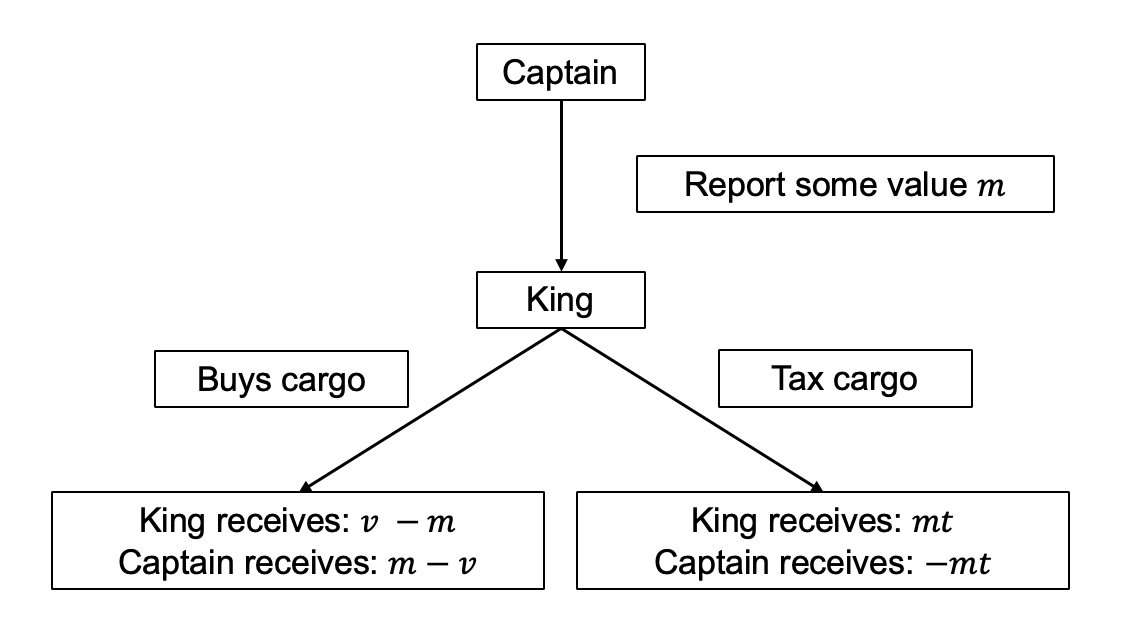
\includegraphics[width = 3.5in]{taxgamertree.png}
\end{figure}

So now we've got a model of the sound dues; let's find the strategies that the king and the captain will play in equilibrium. Why do we care about equilibrium strategy? Well, if we're out of equilibrium, then it means that either the king or the captain can play some other strategy to improve their outcomes. We assume that the agents would have already played an alternative strategy if there is one that improves their payoffs. With that in mind, we introduce the following theorem:

\begin{theorem}
    The king is indifferent between playing buy or tax for any equilibrium message $m$.
\end{theorem}
I will first present an intuitive proof. Suppose that the king prefers to buy the cargo. Then, knowing this, the captain should report a higher value $m$ so that she gets paid more. She should keep on increasing the value until the king is indifferent. Similarly, suppose that the king prefers to tax the cargo, then the captain should report a lower $m$ so she has to pay taxes, and do this until that the king is indifferent. The mathematical proof follows:
\begin{proof}
    Suppose that $v - (1 + t)m > 0$ (i.e., the payoff for the king if he buys the cargo is higher than when he taxes it). Then, there exist some $\epsilon > 0$ such that $m' = m + \epsilon$ and $v - (1 + t)m' > 0$. Thus, the captain can report $m'$ instead of $m$ and gain $m'-v > m - v$, which means that $m$ is not the optimal strategy for the captain, and thus we are not in equilibrium. The proof for when the king prefers taxing the cargo is analogous and is left as an exercise for the reader. 
\end{proof}

Given that the king is indifferent, it follows that the expected payoff that the king gets whether he buys the cargo or not is the same. That is
\begin{align*}
    v - m &= mt \\
    m &= \frac{v}{1 + t}
\end{align*}

We know that as long as the captain plays $m = \frac{v}{1 + t}$, the king would be indifferent. We now check what the king would need to do such that the captain would want to play $m = \frac{v}{1+t}$. Given that the captain has some probability $p(m)$ of playing ``buy", the expected utility of the captain is
\begin{align*}
    EU &= p(m)(m - v) + (1 - p(m))(-tm)
\end{align*}
The captain gets to choose $m$, so we differentiate the equation w.r.t. $m$ and find the optimum
\begin{align*}
    \pd{EU}{m} & = p'(m)(m-v) + p(m) + p'(m)mt -t(1-p(m)) = 0 \\
    & = p'(m)m - p'(m)v + p(m) + p'(m)mt -t + tp(m) = 0
\end{align*}
We know from above that the captain needs to play $m(1+t) = v$ for the king to be indifferent, so we can substitute that in to get
\begin{align*}
    0 & = p'(m)m - p'(m)v + p(m) + p'(m)mt -t + tp(m) \\
    & =  p'(m)m - p'(m)m(1+t)  + p(m) + p'(m)mt -t + tp(m) \\
    & = p(m) -t + tp(m) = 0
\end{align*}
Rearranging gives us
\begin{align*}
    p(m)(1 + t) & = t\\
    p(m) & = \frac{t}{1+t}
\end{align*}
In conclusion, for any given tax rate $t$, the skipper will report $m = \frac{v}{1+t}$, and the king will buy the cargo with probability $\frac{t}{1+t}$ regardless of what was reported. Here, neither player has an incentive to deviate from their current strategy, and thus we have found the Nash equilibrium of the game. 

Since the captain will under-report the true value of their cargo, the mechanism does not induce truth-telling. We see that regardless of what the king plays, he expects to receive $\frac{t}{(1+t)}m$. Thus if the king wants to implement some tax rate $t$, he needs to find tax rate $t^*$ such that $\frac{t^*}{1+t^*} = t$.

More details on this problem can be found in \citet{Haan_2012_Taxation}, but hopefully, this small paragraph gave you a taste of how game-theoretic modeling can be applied to real-life situations. 
\bibliography{bib1}
\end{document}